\documentclass[twoside]{book}

% Packages required by doxygen
\usepackage{calc}
\usepackage{doxygen}
\usepackage{graphicx}
\usepackage[utf8]{inputenc}
\usepackage{makeidx}
\usepackage{multicol}
\usepackage{multirow}
\usepackage{fixltx2e}
\PassOptionsToPackage{warn}{textcomp}
\usepackage{textcomp}
\usepackage[nointegrals]{wasysym}
\usepackage[table]{xcolor}

% Font selection
\usepackage[T1]{fontenc}
\usepackage{mathptmx}
\usepackage[scaled=.90]{helvet}
\usepackage{courier}
\usepackage{amssymb}
\usepackage{sectsty}
\renewcommand{\familydefault}{\sfdefault}
\allsectionsfont{%
  \fontseries{bc}\selectfont%
  \color{darkgray}%
}
\renewcommand{\DoxyLabelFont}{%
  \fontseries{bc}\selectfont%
  \color{darkgray}%
}
\newcommand{\+}{\discretionary{\mbox{\scriptsize$\hookleftarrow$}}{}{}}

% Page & text layout
\usepackage{geometry}
\geometry{%
  a4paper,%
  top=2.5cm,%
  bottom=2.5cm,%
  left=2.5cm,%
  right=2.5cm%
}
\tolerance=750
\hfuzz=15pt
\hbadness=750
\setlength{\emergencystretch}{15pt}
\setlength{\parindent}{0cm}
\setlength{\parskip}{0.2cm}
\makeatletter
\renewcommand{\paragraph}{%
  \@startsection{paragraph}{4}{0ex}{-1.0ex}{1.0ex}{%
    \normalfont\normalsize\bfseries\SS@parafont%
  }%
}
\renewcommand{\subparagraph}{%
  \@startsection{subparagraph}{5}{0ex}{-1.0ex}{1.0ex}{%
    \normalfont\normalsize\bfseries\SS@subparafont%
  }%
}
\makeatother

% Headers & footers
\usepackage{fancyhdr}
\pagestyle{fancyplain}
\fancyhead[LE]{\fancyplain{}{\bfseries\thepage}}
\fancyhead[CE]{\fancyplain{}{}}
\fancyhead[RE]{\fancyplain{}{\bfseries\leftmark}}
\fancyhead[LO]{\fancyplain{}{\bfseries\rightmark}}
\fancyhead[CO]{\fancyplain{}{}}
\fancyhead[RO]{\fancyplain{}{\bfseries\thepage}}
\fancyfoot[LE]{\fancyplain{}{}}
\fancyfoot[CE]{\fancyplain{}{}}
\fancyfoot[RE]{\fancyplain{}{\bfseries\scriptsize Generated on Mon Nov 24 2014 20\+:52\+:53 for My Project by Doxygen }}
\fancyfoot[LO]{\fancyplain{}{\bfseries\scriptsize Generated on Mon Nov 24 2014 20\+:52\+:53 for My Project by Doxygen }}
\fancyfoot[CO]{\fancyplain{}{}}
\fancyfoot[RO]{\fancyplain{}{}}
\renewcommand{\footrulewidth}{0.4pt}
\renewcommand{\chaptermark}[1]{%
  \markboth{#1}{}%
}
\renewcommand{\sectionmark}[1]{%
  \markright{\thesection\ #1}%
}

% Indices & bibliography
\usepackage{natbib}
\usepackage[titles]{tocloft}
\setcounter{tocdepth}{3}
\setcounter{secnumdepth}{5}
\makeindex

% Hyperlinks (required, but should be loaded last)
\usepackage{ifpdf}
\ifpdf
  \usepackage[pdftex,pagebackref=true]{hyperref}
\else
  \usepackage[ps2pdf,pagebackref=true]{hyperref}
\fi
\hypersetup{%
  colorlinks=true,%
  linkcolor=blue,%
  citecolor=blue,%
  unicode%
}

% Custom commands
\newcommand{\clearemptydoublepage}{%
  \newpage{\pagestyle{empty}\cleardoublepage}%
}


%===== C O N T E N T S =====

\begin{document}

% Titlepage & ToC
\hypersetup{pageanchor=false,
             bookmarks=true,
             bookmarksnumbered=true,
             pdfencoding=unicode
            }
\pagenumbering{roman}
\begin{titlepage}
\vspace*{7cm}
\begin{center}%
{\Large My Project }\\
\vspace*{1cm}
{\large Generated by Doxygen 1.8.7}\\
\vspace*{0.5cm}
{\small Mon Nov 24 2014 20:52:53}\\
\end{center}
\end{titlepage}
\clearemptydoublepage
\tableofcontents
\clearemptydoublepage
\pagenumbering{arabic}
\hypersetup{pageanchor=true}

%--- Begin generated contents ---
\chapter{Hierarchical Index}
\section{Class Hierarchy}
This inheritance list is sorted roughly, but not completely, alphabetically\+:\begin{DoxyCompactList}
\item \contentsline{section}{C\+Picture\+:\+:Actor\+Iter}{\pageref{class_c_picture_1_1_actor_iter}}{}
\item \contentsline{section}{C\+Actor}{\pageref{class_c_actor}}{}
\item \contentsline{section}{C\+Actor\+Factory}{\pageref{class_c_actor_factory}}{}
\begin{DoxyCompactList}
\item \contentsline{section}{C\+Harold\+Factory}{\pageref{class_c_harold_factory}}{}
\item \contentsline{section}{C\+Sparty\+Factory}{\pageref{class_c_sparty_factory}}{}
\end{DoxyCompactList}
\item \contentsline{section}{C\+Anim\+Channel}{\pageref{class_c_anim_channel}}{}
\begin{DoxyCompactList}
\item \contentsline{section}{C\+Anim\+Channel\+Angle}{\pageref{class_c_anim_channel_angle}}{}
\item \contentsline{section}{C\+Anim\+Channel\+Point}{\pageref{class_c_anim_channel_point}}{}
\item \contentsline{section}{C\+Anim\+Channel\+Text}{\pageref{class_c_anim_channel_text}}{}
\end{DoxyCompactList}
\item C\+Dialog\begin{DoxyCompactList}
\item \contentsline{section}{C\+Timeline\+Dlg}{\pageref{class_c_timeline_dlg}}{}
\end{DoxyCompactList}
\item C\+Dialog\+Ex\begin{DoxyCompactList}
\item \contentsline{section}{C\+About\+Dlg}{\pageref{class_c_about_dlg}}{}
\end{DoxyCompactList}
\item \contentsline{section}{C\+Drawable}{\pageref{class_c_drawable}}{}
\begin{DoxyCompactList}
\item \contentsline{section}{C\+Image\+Drawable}{\pageref{class_c_image_drawable}}{}
\begin{DoxyCompactList}
\item \contentsline{section}{C\+Head\+Top}{\pageref{class_c_head_top}}{}
\item \contentsline{section}{C\+Knife}{\pageref{class_c_knife}}{}
\end{DoxyCompactList}
\item \contentsline{section}{C\+Poly\+Drawable}{\pageref{class_c_poly_drawable}}{}
\item \contentsline{section}{C\+Text\+Bubble\+Drawable}{\pageref{class_c_text_bubble_drawable}}{}
\end{DoxyCompactList}
\item C\+Frame\+Wnd\+Ex\begin{DoxyCompactList}
\item \contentsline{section}{C\+Main\+Frame}{\pageref{class_c_main_frame}}{}
\end{DoxyCompactList}
\item \contentsline{section}{C\+Drawable\+:\+:Child\+Iter}{\pageref{class_c_drawable_1_1_child_iter}}{}
\item \contentsline{section}{xmlnode\+:\+:C\+Xml\+Node\+:\+:Children}{\pageref{classxmlnode_1_1_c_xml_node_1_1_children}}{}
\item \contentsline{section}{C\+Linked\+List}{\pageref{class_c_linked_list}}{}
\item \contentsline{section}{C\+Particle\+System}{\pageref{class_c_particle_system}}{}
\item \contentsline{section}{C\+Picture}{\pageref{class_c_picture}}{}
\item \contentsline{section}{C\+Picture\+Factory}{\pageref{class_c_picture_factory}}{}
\item \contentsline{section}{C\+Picture\+Observer}{\pageref{class_c_picture_observer}}{}
\begin{DoxyCompactList}
\item \contentsline{section}{C\+View\+Actors}{\pageref{class_c_view_actors}}{}
\item \contentsline{section}{C\+View\+Edit}{\pageref{class_c_view_edit}}{}
\item \contentsline{section}{C\+View\+Timeline}{\pageref{class_c_view_timeline}}{}
\end{DoxyCompactList}
\item \contentsline{section}{C\+Rotated\+Bitmap}{\pageref{class_c_rotated_bitmap}}{}
\begin{DoxyCompactList}
\item \contentsline{section}{C\+Image\+Drawable}{\pageref{class_c_image_drawable}}{}
\end{DoxyCompactList}
\item C\+Scroll\+View\begin{DoxyCompactList}
\item \contentsline{section}{C\+View\+Actors}{\pageref{class_c_view_actors}}{}
\item \contentsline{section}{C\+View\+Edit}{\pageref{class_c_view_edit}}{}
\item \contentsline{section}{C\+View\+Timeline}{\pageref{class_c_view_timeline}}{}
\end{DoxyCompactList}
\item \contentsline{section}{C\+Snowflake}{\pageref{class_c_snowflake}}{}
\item \contentsline{section}{C\+Timeline}{\pageref{class_c_timeline}}{}
\item C\+View\begin{DoxyCompactList}
\item \contentsline{section}{C\+View\+Top}{\pageref{class_c_view_top}}{}
\end{DoxyCompactList}
\item C\+Win\+App\begin{DoxyCompactList}
\item \contentsline{section}{C\+Canadian\+Experience\+App}{\pageref{class_c_canadian_experience_app}}{}
\end{DoxyCompactList}
\item \contentsline{section}{xmlnode\+:\+:C\+Xml\+Node}{\pageref{classxmlnode_1_1_c_xml_node}}{}
\item exception\begin{DoxyCompactList}
\item \contentsline{section}{xmlnode\+:\+:C\+Xml\+Node\+:\+:Exception}{\pageref{classxmlnode_1_1_c_xml_node_1_1_exception}}{}
\end{DoxyCompactList}
\item \contentsline{section}{xmlnode\+:\+:C\+Xml\+Node\+:\+:Iterator}{\pageref{classxmlnode_1_1_c_xml_node_1_1_iterator}}{}
\item Keyframe\begin{DoxyCompactList}
\item \contentsline{section}{C\+Anim\+Channel\+Angle\+:\+:Keyframe\+Angle}{\pageref{class_c_anim_channel_angle_1_1_keyframe_angle}}{}
\end{DoxyCompactList}
\item \contentsline{section}{C\+Anim\+Channel\+:\+:Keyframe}{\pageref{class_c_anim_channel_1_1_keyframe}}{}
\begin{DoxyCompactList}
\item \contentsline{section}{C\+Anim\+Channel\+Point\+:\+:Keyframe\+Point}{\pageref{class_c_anim_channel_point_1_1_keyframe_point}}{}
\item \contentsline{section}{C\+Anim\+Channel\+Text\+:\+:Keyframe\+Text}{\pageref{class_c_anim_channel_text_1_1_keyframe_text}}{}
\end{DoxyCompactList}
\end{DoxyCompactList}

\chapter{Class Index}
\section{Class List}
Here are the classes, structs, unions and interfaces with brief descriptions\+:\begin{DoxyCompactList}
\item\contentsline{section}{\hyperlink{class_c_picture_1_1_actor_iter}{C\+Picture\+::\+Actor\+Iter} \\*Iterator that iterates over the actors in a picture }{\pageref{class_c_picture_1_1_actor_iter}}{}
\item\contentsline{section}{\hyperlink{class_c_about_dlg}{C\+About\+Dlg} \\*The About dialog box }{\pageref{class_c_about_dlg}}{}
\item\contentsline{section}{\hyperlink{class_c_actor}{C\+Actor} \\*Class for actors in our drawings }{\pageref{class_c_actor}}{}
\item\contentsline{section}{\hyperlink{class_c_actor_factory}{C\+Actor\+Factory} \\*Abstract base class for actor factories }{\pageref{class_c_actor_factory}}{}
\item\contentsline{section}{\hyperlink{class_c_anim_channel}{C\+Anim\+Channel} \\*Base class for an animation channel }{\pageref{class_c_anim_channel}}{}
\item\contentsline{section}{\hyperlink{class_c_anim_channel_angle}{C\+Anim\+Channel\+Angle} \\*Animation channel for angles }{\pageref{class_c_anim_channel_angle}}{}
\item\contentsline{section}{\hyperlink{class_c_anim_channel_point}{C\+Anim\+Channel\+Point} \\*An animation channel specific to points (movement) }{\pageref{class_c_anim_channel_point}}{}
\item\contentsline{section}{\hyperlink{class_c_anim_channel_text}{C\+Anim\+Channel\+Text} }{\pageref{class_c_anim_channel_text}}{}
\item\contentsline{section}{\hyperlink{class_c_canadian_experience_app}{C\+Canadian\+Experience\+App} \\*Program application class }{\pageref{class_c_canadian_experience_app}}{}
\item\contentsline{section}{\hyperlink{class_c_drawable}{C\+Drawable} \\*Abstract base class for drawable elements of our picture }{\pageref{class_c_drawable}}{}
\item\contentsline{section}{\hyperlink{class_c_harold_factory}{C\+Harold\+Factory} \\*Factory class that builds the Harold character }{\pageref{class_c_harold_factory}}{}
\item\contentsline{section}{\hyperlink{class_c_head_top}{C\+Head\+Top} \\*Implements the top of a characters head, which has special functionality }{\pageref{class_c_head_top}}{}
\item\contentsline{section}{\hyperlink{class_c_drawable_1_1_child_iter}{C\+Drawable\+::\+Child\+Iter} \\*Iterator that iterates over the children of this drawable }{\pageref{class_c_drawable_1_1_child_iter}}{}
\item\contentsline{section}{\hyperlink{classxmlnode_1_1_c_xml_node_1_1_children}{xmlnode\+::\+C\+Xml\+Node\+::\+Children} \\*Representation of children to support iteration }{\pageref{classxmlnode_1_1_c_xml_node_1_1_children}}{}
\item\contentsline{section}{\hyperlink{class_c_image_drawable}{C\+Image\+Drawable} \\*A drawable based on drawing a bitmap image }{\pageref{class_c_image_drawable}}{}
\item\contentsline{section}{\hyperlink{class_c_knife}{C\+Knife} \\*Implemnet the knife for sparty }{\pageref{class_c_knife}}{}
\item\contentsline{section}{\hyperlink{class_c_linked_list}{C\+Linked\+List} \\*The linked calss to store the snow flakes }{\pageref{class_c_linked_list}}{}
\item\contentsline{section}{\hyperlink{class_c_main_frame}{C\+Main\+Frame} \\*Program main frame }{\pageref{class_c_main_frame}}{}
\item\contentsline{section}{\hyperlink{class_c_particle_system}{C\+Particle\+System} \\*The Particle\+System to implement the snow draw and update }{\pageref{class_c_particle_system}}{}
\item\contentsline{section}{\hyperlink{class_c_picture}{C\+Picture} \\*The picture we are drawing }{\pageref{class_c_picture}}{}
\item\contentsline{section}{\hyperlink{class_c_picture_factory}{C\+Picture\+Factory} \\*A factory class that builds our picture }{\pageref{class_c_picture_factory}}{}
\item\contentsline{section}{\hyperlink{class_c_picture_observer}{C\+Picture\+Observer} \\*Observer base class for a picture }{\pageref{class_c_picture_observer}}{}
\item\contentsline{section}{\hyperlink{class_c_poly_drawable}{C\+Poly\+Drawable} \\*A drawable based on polygon images }{\pageref{class_c_poly_drawable}}{}
\item\contentsline{section}{\hyperlink{class_c_rotated_bitmap}{C\+Rotated\+Bitmap} \\*Base class for a rotated bitmap }{\pageref{class_c_rotated_bitmap}}{}
\item\contentsline{section}{\hyperlink{class_c_snowflake}{C\+Snowflake} \\*The snow flake class to implement snow }{\pageref{class_c_snowflake}}{}
\item\contentsline{section}{\hyperlink{class_c_sparty_factory}{C\+Sparty\+Factory} \\*Factory that builds the Sparty actor }{\pageref{class_c_sparty_factory}}{}
\item\contentsline{section}{\hyperlink{class_c_text_bubble_drawable}{C\+Text\+Bubble\+Drawable} \\*The text bubble class adpater }{\pageref{class_c_text_bubble_drawable}}{}
\item\contentsline{section}{\hyperlink{class_c_timeline}{C\+Timeline} \\*The animation timeline class }{\pageref{class_c_timeline}}{}
\item\contentsline{section}{\hyperlink{class_c_timeline_dlg}{C\+Timeline\+Dlg} \\*The timeline parameters dialog box }{\pageref{class_c_timeline_dlg}}{}
\item\contentsline{section}{\hyperlink{class_c_view_actors}{C\+View\+Actors} \\*Class that provides a view windows for actors }{\pageref{class_c_view_actors}}{}
\item\contentsline{section}{\hyperlink{class_c_view_edit}{C\+View\+Edit} \\*View class the provides a window for editing our pixture }{\pageref{class_c_view_edit}}{}
\item\contentsline{section}{\hyperlink{class_c_view_timeline}{C\+View\+Timeline} \\*View window for the animation timeline }{\pageref{class_c_view_timeline}}{}
\item\contentsline{section}{\hyperlink{class_c_view_top}{C\+View\+Top} \\*Top of the screen view }{\pageref{class_c_view_top}}{}
\item\contentsline{section}{\hyperlink{classxmlnode_1_1_c_xml_node}{xmlnode\+::\+C\+Xml\+Node} \\*A wrapper for msxml nodes }{\pageref{classxmlnode_1_1_c_xml_node}}{}
\item\contentsline{section}{\hyperlink{classxmlnode_1_1_c_xml_node_1_1_exception}{xmlnode\+::\+C\+Xml\+Node\+::\+Exception} \\*Exceptions for \hyperlink{classxmlnode_1_1_c_xml_node}{C\+Xml\+Node} }{\pageref{classxmlnode_1_1_c_xml_node_1_1_exception}}{}
\item\contentsline{section}{\hyperlink{classxmlnode_1_1_c_xml_node_1_1_iterator}{xmlnode\+::\+C\+Xml\+Node\+::\+Iterator} \\*Support for iterating over the children of a node }{\pageref{classxmlnode_1_1_c_xml_node_1_1_iterator}}{}
\item\contentsline{section}{\hyperlink{class_c_anim_channel_1_1_keyframe}{C\+Anim\+Channel\+::\+Keyframe} \\*Class that represents a keyframe }{\pageref{class_c_anim_channel_1_1_keyframe}}{}
\item\contentsline{section}{\hyperlink{class_c_anim_channel_angle_1_1_keyframe_angle}{C\+Anim\+Channel\+Angle\+::\+Keyframe\+Angle} \\*A keyframe for an angle channel }{\pageref{class_c_anim_channel_angle_1_1_keyframe_angle}}{}
\item\contentsline{section}{\hyperlink{class_c_anim_channel_point_1_1_keyframe_point}{C\+Anim\+Channel\+Point\+::\+Keyframe\+Point} \\*A keyframe for a point channel }{\pageref{class_c_anim_channel_point_1_1_keyframe_point}}{}
\item\contentsline{section}{\hyperlink{class_c_anim_channel_text_1_1_keyframe_text}{C\+Anim\+Channel\+Text\+::\+Keyframe\+Text} \\*A ket frame for the text channel }{\pageref{class_c_anim_channel_text_1_1_keyframe_text}}{}
\end{DoxyCompactList}

\chapter{File Index}
\section{File List}
Here is a list of all documented files with brief descriptions\+:\begin{DoxyCompactList}
\item\contentsline{section}{\hyperlink{_actor_8cpp}{Actor.\+cpp} }{\pageref{_actor_8cpp}}{}
\item\contentsline{section}{\hyperlink{_actor_8h}{Actor.\+h} \\*Class for actors in our drawings }{\pageref{_actor_8h}}{}
\item\contentsline{section}{\hyperlink{_actor_factory_8cpp}{Actor\+Factory.\+cpp} }{\pageref{_actor_factory_8cpp}}{}
\item\contentsline{section}{\hyperlink{_actor_factory_8h}{Actor\+Factory.\+h} \\*Abstract base class for actor factories }{\pageref{_actor_factory_8h}}{}
\item\contentsline{section}{\hyperlink{_anim_channel_8cpp}{Anim\+Channel.\+cpp} }{\pageref{_anim_channel_8cpp}}{}
\item\contentsline{section}{\hyperlink{_anim_channel_8h}{Anim\+Channel.\+h} \\*Base class for an animation channel }{\pageref{_anim_channel_8h}}{}
\item\contentsline{section}{\hyperlink{_anim_channel_angle_8cpp}{Anim\+Channel\+Angle.\+cpp} }{\pageref{_anim_channel_angle_8cpp}}{}
\item\contentsline{section}{\hyperlink{_anim_channel_angle_8h}{Anim\+Channel\+Angle.\+h} \\*Animation channel for angles }{\pageref{_anim_channel_angle_8h}}{}
\item\contentsline{section}{\hyperlink{_anim_channel_point_8cpp}{Anim\+Channel\+Point.\+cpp} }{\pageref{_anim_channel_point_8cpp}}{}
\item\contentsline{section}{\hyperlink{_anim_channel_point_8h}{Anim\+Channel\+Point.\+h} \\*An animation channel specific to points (movement) }{\pageref{_anim_channel_point_8h}}{}
\item\contentsline{section}{\hyperlink{_anim_channel_text_8cpp}{Anim\+Channel\+Text.\+cpp} }{\pageref{_anim_channel_text_8cpp}}{}
\item\contentsline{section}{\hyperlink{_anim_channel_text_8h}{Anim\+Channel\+Text.\+h} \\*The Anim\+Channel Class to edit the text in the text bubble during the animation }{\pageref{_anim_channel_text_8h}}{}
\item\contentsline{section}{\hyperlink{_canadian_experience_8cpp}{Canadian\+Experience.\+cpp} }{\pageref{_canadian_experience_8cpp}}{}
\item\contentsline{section}{\hyperlink{_canadian_experience_8h}{Canadian\+Experience.\+h} \\*Program application class }{\pageref{_canadian_experience_8h}}{}
\item\contentsline{section}{\hyperlink{_double_buffer_d_c_8h}{Double\+Buffer\+D\+C.\+h} \\*Customer device context that supports double buffering }{\pageref{_double_buffer_d_c_8h}}{}
\item\contentsline{section}{\hyperlink{_drawable_8cpp}{Drawable.\+cpp} }{\pageref{_drawable_8cpp}}{}
\item\contentsline{section}{\hyperlink{_drawable_8h}{Drawable.\+h} \\*Abstract base class for drawable elements of our picture }{\pageref{_drawable_8h}}{}
\item\contentsline{section}{\hyperlink{_harold_factory_8cpp}{Harold\+Factory.\+cpp} }{\pageref{_harold_factory_8cpp}}{}
\item\contentsline{section}{\hyperlink{_harold_factory_8h}{Harold\+Factory.\+h} \\*Factory class that builds the Harold character }{\pageref{_harold_factory_8h}}{}
\item\contentsline{section}{\hyperlink{_head_top_8h}{Head\+Top.\+h} \\*Implements the top of a characters head, which has special functionality }{\pageref{_head_top_8h}}{}
\item\contentsline{section}{\hyperlink{_image_drawable_8cpp}{Image\+Drawable.\+cpp} }{\pageref{_image_drawable_8cpp}}{}
\item\contentsline{section}{\hyperlink{_image_drawable_8h}{Image\+Drawable.\+h} \\*A drawable based on drawing a bitmap image }{\pageref{_image_drawable_8h}}{}
\item\contentsline{section}{\hyperlink{_knife_8cpp}{Knife.\+cpp} }{\pageref{_knife_8cpp}}{}
\item\contentsline{section}{\hyperlink{_knife_8h}{Knife.\+h} \\*Implement a knife for sparty }{\pageref{_knife_8h}}{}
\item\contentsline{section}{\hyperlink{_linked_list_8cpp}{Linked\+List.\+cpp} }{\pageref{_linked_list_8cpp}}{}
\item\contentsline{section}{\hyperlink{_linked_list_8h}{Linked\+List.\+h} \\*The linked list to store the snowflake }{\pageref{_linked_list_8h}}{}
\item\contentsline{section}{\hyperlink{_main_frm_8cpp}{Main\+Frm.\+cpp} }{\pageref{_main_frm_8cpp}}{}
\item\contentsline{section}{\hyperlink{_main_frm_8h}{Main\+Frm.\+h} \\*The program main frame }{\pageref{_main_frm_8h}}{}
\item\contentsline{section}{\hyperlink{_particle_system_8cpp}{Particle\+System.\+cpp} }{\pageref{_particle_system_8cpp}}{}
\item\contentsline{section}{\hyperlink{_particle_system_8h}{Particle\+System.\+h} \\*Class for particle syystem of snow operation }{\pageref{_particle_system_8h}}{}
\item\contentsline{section}{\hyperlink{_picture_8cpp}{Picture.\+cpp} }{\pageref{_picture_8cpp}}{}
\item\contentsline{section}{\hyperlink{_picture_8h}{Picture.\+h} \\*The picture we are drawing }{\pageref{_picture_8h}}{}
\item\contentsline{section}{\hyperlink{_picture_factory_8cpp}{Picture\+Factory.\+cpp} }{\pageref{_picture_factory_8cpp}}{}
\item\contentsline{section}{\hyperlink{_picture_factory_8h}{Picture\+Factory.\+h} \\*A factory class that builds our picture }{\pageref{_picture_factory_8h}}{}
\item\contentsline{section}{\hyperlink{_picture_observer_8cpp}{Picture\+Observer.\+cpp} }{\pageref{_picture_observer_8cpp}}{}
\item\contentsline{section}{\hyperlink{_picture_observer_8h}{Picture\+Observer.\+h} \\*Observer base class for a picture }{\pageref{_picture_observer_8h}}{}
\item\contentsline{section}{\hyperlink{_poly_drawable_8cpp}{Poly\+Drawable.\+cpp} }{\pageref{_poly_drawable_8cpp}}{}
\item\contentsline{section}{\hyperlink{_poly_drawable_8h}{Poly\+Drawable.\+h} \\*A drawable based on polygon images }{\pageref{_poly_drawable_8h}}{}
\item\contentsline{section}{{\bfseries resource.\+h} }{\pageref{resource_8h}}{}
\item\contentsline{section}{\hyperlink{_rotated_bitmap_8cpp}{Rotated\+Bitmap.\+cpp} }{\pageref{_rotated_bitmap_8cpp}}{}
\item\contentsline{section}{\hyperlink{_rotated_bitmap_8h}{Rotated\+Bitmap.\+h} \\*Base class for a rotated bitmap }{\pageref{_rotated_bitmap_8h}}{}
\item\contentsline{section}{\hyperlink{_snowflake_8cpp}{Snowflake.\+cpp} }{\pageref{_snowflake_8cpp}}{}
\item\contentsline{section}{\hyperlink{_snowflake_8h}{Snowflake.\+h} \\*The snowfalke class to inplement the snow }{\pageref{_snowflake_8h}}{}
\item\contentsline{section}{\hyperlink{_sparty_factory_8cpp}{Sparty\+Factory.\+cpp} }{\pageref{_sparty_factory_8cpp}}{}
\item\contentsline{section}{\hyperlink{_sparty_factory_8h}{Sparty\+Factory.\+h} \\*Factory that builds the Sparty actor }{\pageref{_sparty_factory_8h}}{}
\item\contentsline{section}{{\bfseries stdafx.\+h} }{\pageref{stdafx_8h}}{}
\item\contentsline{section}{{\bfseries targetver.\+h} }{\pageref{targetver_8h}}{}
\item\contentsline{section}{\hyperlink{_text_bubble_drawable_8cpp}{Text\+Bubble\+Drawable.\+cpp} }{\pageref{_text_bubble_drawable_8cpp}}{}
\item\contentsline{section}{\hyperlink{_text_bubble_drawable_8h}{Text\+Bubble\+Drawable.\+h} \\*The Text Bubble adapater class derived from the Drawable class }{\pageref{_text_bubble_drawable_8h}}{}
\item\contentsline{section}{\hyperlink{_timeline_8cpp}{Timeline.\+cpp} }{\pageref{_timeline_8cpp}}{}
\item\contentsline{section}{\hyperlink{_timeline_8h}{Timeline.\+h} \\*The animation timeline class }{\pageref{_timeline_8h}}{}
\item\contentsline{section}{\hyperlink{_timeline_dlg_8cpp}{Timeline\+Dlg.\+cpp} }{\pageref{_timeline_dlg_8cpp}}{}
\item\contentsline{section}{\hyperlink{_timeline_dlg_8h}{Timeline\+Dlg.\+h} \\*The timeline parameters dialog box }{\pageref{_timeline_dlg_8h}}{}
\item\contentsline{section}{\hyperlink{_view_actors_8cpp}{View\+Actors.\+cpp} }{\pageref{_view_actors_8cpp}}{}
\item\contentsline{section}{\hyperlink{_view_actors_8h}{View\+Actors.\+h} \\*Class that provides a view windows for actors }{\pageref{_view_actors_8h}}{}
\item\contentsline{section}{\hyperlink{_view_edit_8cpp}{View\+Edit.\+cpp} }{\pageref{_view_edit_8cpp}}{}
\item\contentsline{section}{\hyperlink{_view_edit_8h}{View\+Edit.\+h} \\*View class the provides a window for editing our pixture }{\pageref{_view_edit_8h}}{}
\item\contentsline{section}{\hyperlink{_view_timeline_8cpp}{View\+Timeline.\+cpp} }{\pageref{_view_timeline_8cpp}}{}
\item\contentsline{section}{\hyperlink{_view_timeline_8h}{View\+Timeline.\+h} \\*View window for the animation timeline }{\pageref{_view_timeline_8h}}{}
\item\contentsline{section}{\hyperlink{_view_top_8cpp}{View\+Top.\+cpp} }{\pageref{_view_top_8cpp}}{}
\item\contentsline{section}{\hyperlink{_view_top_8h}{View\+Top.\+h} \\*Class for the top of the screen view }{\pageref{_view_top_8h}}{}
\item\contentsline{section}{\hyperlink{_xml_node_8cpp}{Xml\+Node.\+cpp} \\*Class that implements a wrapper for msxml nodes }{\pageref{_xml_node_8cpp}}{}
\item\contentsline{section}{\hyperlink{_xml_node_8h}{Xml\+Node.\+h} \\*Class that implements a wrapper for msxml nodes }{\pageref{_xml_node_8h}}{}
\end{DoxyCompactList}

\chapter{Class Documentation}
\hypertarget{class_c_picture_1_1_actor_iter}{\section{C\+Picture\+:\+:Actor\+Iter Class Reference}
\label{class_c_picture_1_1_actor_iter}\index{C\+Picture\+::\+Actor\+Iter@{C\+Picture\+::\+Actor\+Iter}}
}


Iterator that iterates over the actors in a picture.  




{\ttfamily \#include $<$Picture.\+h$>$}

\subsection*{Public Member Functions}
\begin{DoxyCompactItemize}
\item 
\hyperlink{class_c_picture_1_1_actor_iter_a2f2f57be59c8599af1e2c304272d2deb}{Actor\+Iter} (\hyperlink{class_c_picture}{C\+Picture} $\ast$picture, int pos)
\begin{DoxyCompactList}\small\item\em Constructor. \end{DoxyCompactList}\item 
bool \hyperlink{class_c_picture_1_1_actor_iter_a68cc04a07bd5766b1d7b0ca0c0bcb856}{operator!=} (const \hyperlink{class_c_picture_1_1_actor_iter}{Actor\+Iter} \&other) const 
\begin{DoxyCompactList}\small\item\em Test for end of the iterator. \end{DoxyCompactList}\item 
std\+::shared\+\_\+ptr$<$ \hyperlink{class_c_actor}{C\+Actor} $>$ \hyperlink{class_c_picture_1_1_actor_iter_a7401edfaeb0f0fb2ff54df57d84a3777}{operator$\ast$} () const 
\begin{DoxyCompactList}\small\item\em Get value at current position. \end{DoxyCompactList}\item 
const \hyperlink{class_c_picture_1_1_actor_iter}{Actor\+Iter} \& \hyperlink{class_c_picture_1_1_actor_iter_a8e52080b2ce8a1f12e2dfcef310b2164}{operator++} ()
\begin{DoxyCompactList}\small\item\em Increment the iterator. \end{DoxyCompactList}\end{DoxyCompactItemize}


\subsection{Detailed Description}
Iterator that iterates over the actors in a picture. 

\subsection{Constructor \& Destructor Documentation}
\hypertarget{class_c_picture_1_1_actor_iter_a2f2f57be59c8599af1e2c304272d2deb}{\index{C\+Picture\+::\+Actor\+Iter@{C\+Picture\+::\+Actor\+Iter}!Actor\+Iter@{Actor\+Iter}}
\index{Actor\+Iter@{Actor\+Iter}!C\+Picture\+::\+Actor\+Iter@{C\+Picture\+::\+Actor\+Iter}}
\subsubsection[{Actor\+Iter}]{\setlength{\rightskip}{0pt plus 5cm}C\+Picture\+::\+Actor\+Iter\+::\+Actor\+Iter (
\begin{DoxyParamCaption}
\item[{{\bf C\+Picture} $\ast$}]{picture, }
\item[{int}]{pos}
\end{DoxyParamCaption}
)\hspace{0.3cm}{\ttfamily [inline]}}}\label{class_c_picture_1_1_actor_iter_a2f2f57be59c8599af1e2c304272d2deb}


Constructor. 


\begin{DoxyParams}{Parameters}
{\em picture} & Picture we are iterating \\
\hline
{\em pos} & Starting position \\
\hline
\end{DoxyParams}


\subsection{Member Function Documentation}
\hypertarget{class_c_picture_1_1_actor_iter_a68cc04a07bd5766b1d7b0ca0c0bcb856}{\index{C\+Picture\+::\+Actor\+Iter@{C\+Picture\+::\+Actor\+Iter}!operator"!=@{operator"!=}}
\index{operator"!=@{operator"!=}!C\+Picture\+::\+Actor\+Iter@{C\+Picture\+::\+Actor\+Iter}}
\subsubsection[{operator"!=}]{\setlength{\rightskip}{0pt plus 5cm}bool C\+Picture\+::\+Actor\+Iter\+::operator!= (
\begin{DoxyParamCaption}
\item[{const {\bf Actor\+Iter} \&}]{other}
\end{DoxyParamCaption}
) const\hspace{0.3cm}{\ttfamily [inline]}}}\label{class_c_picture_1_1_actor_iter_a68cc04a07bd5766b1d7b0ca0c0bcb856}


Test for end of the iterator. 


\begin{DoxyParams}{Parameters}
{\em other} & Other object to test against \\
\hline
\end{DoxyParams}
\begin{DoxyReturn}{Returns}
True if we this position equals not equal to the other position 
\end{DoxyReturn}
\hypertarget{class_c_picture_1_1_actor_iter_a7401edfaeb0f0fb2ff54df57d84a3777}{\index{C\+Picture\+::\+Actor\+Iter@{C\+Picture\+::\+Actor\+Iter}!operator$\ast$@{operator$\ast$}}
\index{operator$\ast$@{operator$\ast$}!C\+Picture\+::\+Actor\+Iter@{C\+Picture\+::\+Actor\+Iter}}
\subsubsection[{operator$\ast$}]{\setlength{\rightskip}{0pt plus 5cm}std\+::shared\+\_\+ptr$<${\bf C\+Actor}$>$ C\+Picture\+::\+Actor\+Iter\+::operator$\ast$ (
\begin{DoxyParamCaption}
{}
\end{DoxyParamCaption}
) const\hspace{0.3cm}{\ttfamily [inline]}}}\label{class_c_picture_1_1_actor_iter_a7401edfaeb0f0fb2ff54df57d84a3777}


Get value at current position. 

\begin{DoxyReturn}{Returns}
Value at m\+Pos in the collection 
\end{DoxyReturn}
\hypertarget{class_c_picture_1_1_actor_iter_a8e52080b2ce8a1f12e2dfcef310b2164}{\index{C\+Picture\+::\+Actor\+Iter@{C\+Picture\+::\+Actor\+Iter}!operator++@{operator++}}
\index{operator++@{operator++}!C\+Picture\+::\+Actor\+Iter@{C\+Picture\+::\+Actor\+Iter}}
\subsubsection[{operator++}]{\setlength{\rightskip}{0pt plus 5cm}const {\bf Actor\+Iter}\& C\+Picture\+::\+Actor\+Iter\+::operator++ (
\begin{DoxyParamCaption}
{}
\end{DoxyParamCaption}
)\hspace{0.3cm}{\ttfamily [inline]}}}\label{class_c_picture_1_1_actor_iter_a8e52080b2ce8a1f12e2dfcef310b2164}


Increment the iterator. 

\begin{DoxyReturn}{Returns}
Reference to this iterator 
\end{DoxyReturn}


The documentation for this class was generated from the following file\+:\begin{DoxyCompactItemize}
\item 
\hyperlink{_picture_8h}{Picture.\+h}\end{DoxyCompactItemize}

\hypertarget{class_c_about_dlg}{\section{C\+About\+Dlg Class Reference}
\label{class_c_about_dlg}\index{C\+About\+Dlg@{C\+About\+Dlg}}
}


The About dialog box.  


Inheritance diagram for C\+About\+Dlg\+:\begin{figure}[H]
\begin{center}
\leavevmode
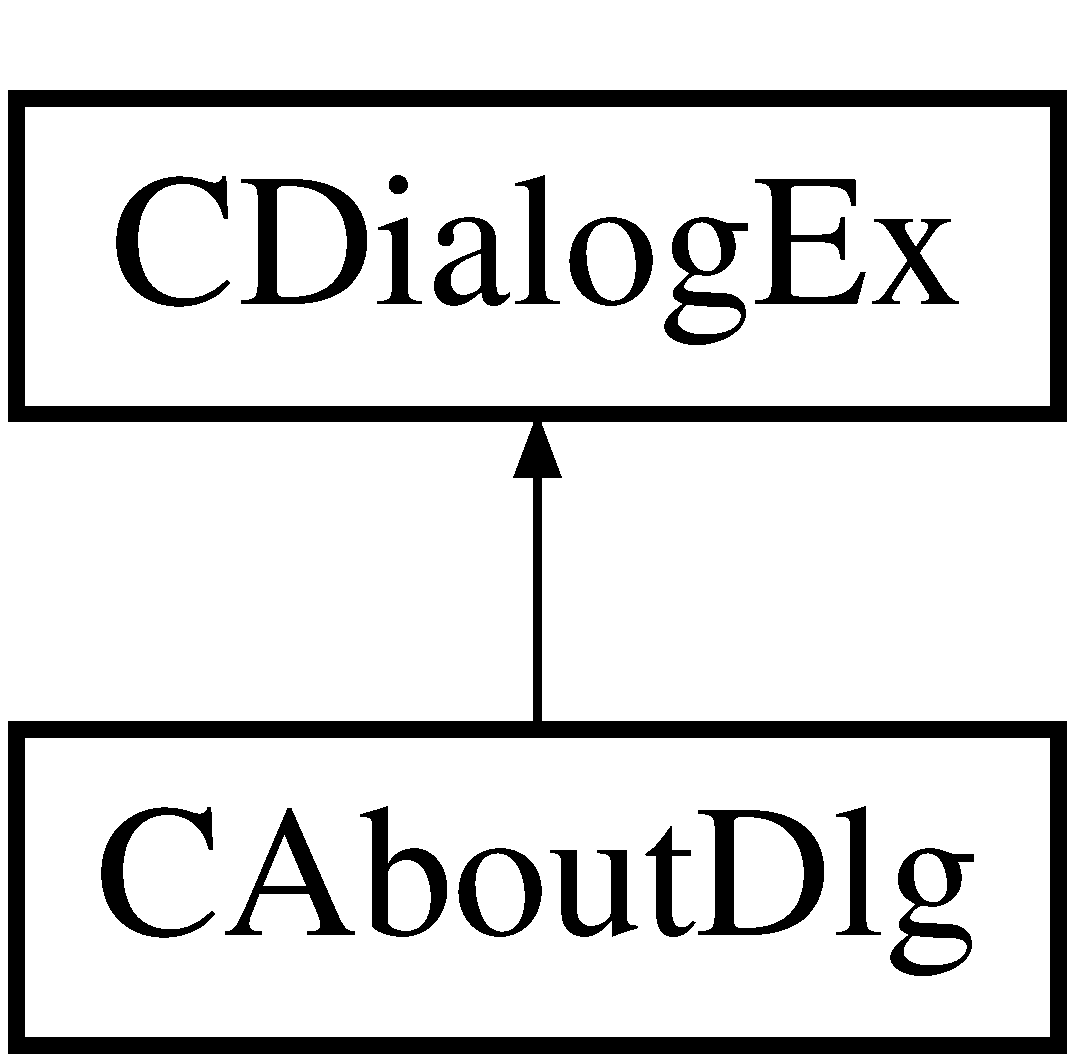
\includegraphics[height=2.000000cm]{class_c_about_dlg}
\end{center}
\end{figure}
\subsection*{Public Types}
\begin{DoxyCompactItemize}
\item 
\hypertarget{class_c_about_dlg_a27a5d4c47f16acb8562522fcd22871f7}{enum \{ {\bfseries I\+D\+D} = I\+D\+D\+\_\+\+A\+B\+O\+U\+T\+B\+O\+X
 \}}\label{class_c_about_dlg_a27a5d4c47f16acb8562522fcd22871f7}

\end{DoxyCompactItemize}
\subsection*{Public Member Functions}
\begin{DoxyCompactItemize}
\item 
\hypertarget{class_c_about_dlg_a6d1e6a33fef23bee6e75254189d865ce}{\hyperlink{class_c_about_dlg_a6d1e6a33fef23bee6e75254189d865ce}{C\+About\+Dlg} ()}\label{class_c_about_dlg_a6d1e6a33fef23bee6e75254189d865ce}

\begin{DoxyCompactList}\small\item\em Constructor. \end{DoxyCompactList}\end{DoxyCompactItemize}
\subsection*{Protected Member Functions}
\begin{DoxyCompactItemize}
\item 
virtual void \hyperlink{class_c_about_dlg_ab83db7484fec957282d7d5a21aed4df4}{Do\+Data\+Exchange} (C\+Data\+Exchange $\ast$p\+D\+X)
\begin{DoxyCompactList}\small\item\em Exchange data between the class and the dialog box. \end{DoxyCompactList}\end{DoxyCompactItemize}


\subsection{Detailed Description}
The About dialog box. 

\subsection{Member Function Documentation}
\hypertarget{class_c_about_dlg_ab83db7484fec957282d7d5a21aed4df4}{\index{C\+About\+Dlg@{C\+About\+Dlg}!Do\+Data\+Exchange@{Do\+Data\+Exchange}}
\index{Do\+Data\+Exchange@{Do\+Data\+Exchange}!C\+About\+Dlg@{C\+About\+Dlg}}
\subsubsection[{Do\+Data\+Exchange}]{\setlength{\rightskip}{0pt plus 5cm}void C\+About\+Dlg\+::\+Do\+Data\+Exchange (
\begin{DoxyParamCaption}
\item[{C\+Data\+Exchange $\ast$}]{p\+D\+X}
\end{DoxyParamCaption}
)\hspace{0.3cm}{\ttfamily [protected]}, {\ttfamily [virtual]}}}\label{class_c_about_dlg_ab83db7484fec957282d7d5a21aed4df4}


Exchange data between the class and the dialog box. 


\begin{DoxyParams}{Parameters}
{\em p\+D\+X} & structure that controls the data exchange \\
\hline
\end{DoxyParams}


The documentation for this class was generated from the following file\+:\begin{DoxyCompactItemize}
\item 
\hyperlink{_canadian_experience_8cpp}{Canadian\+Experience.\+cpp}\end{DoxyCompactItemize}

\hypertarget{class_c_actor}{\section{C\+Actor Class Reference}
\label{class_c_actor}\index{C\+Actor@{C\+Actor}}
}


Class for actors in our drawings.  




{\ttfamily \#include $<$Actor.\+h$>$}

\subsection*{Public Member Functions}
\begin{DoxyCompactItemize}
\item 
\hyperlink{class_c_actor_a2849f9370b66ddeaa727c8b7045d62c2}{C\+Actor} (const std\+::wstring \&name)
\begin{DoxyCompactList}\small\item\em Constructor. \end{DoxyCompactList}\item 
\hypertarget{class_c_actor_ae7683d5f0b3edc85dc47850fa71de40f}{\hyperlink{class_c_actor_ae7683d5f0b3edc85dc47850fa71de40f}{C\+Actor} ()=delete}\label{class_c_actor_ae7683d5f0b3edc85dc47850fa71de40f}

\begin{DoxyCompactList}\small\item\em Default constructor disabled. \end{DoxyCompactList}\item 
\hypertarget{class_c_actor_a8af986ad4ec530967f942aaebd853632}{\hyperlink{class_c_actor_a8af986ad4ec530967f942aaebd853632}{C\+Actor} (const \hyperlink{class_c_actor}{C\+Actor} \&)=delete}\label{class_c_actor_a8af986ad4ec530967f942aaebd853632}

\begin{DoxyCompactList}\small\item\em Copy constructor disabled. \end{DoxyCompactList}\item 
\hypertarget{class_c_actor_aa947810cfb2f45129b501296bcad837c}{void \hyperlink{class_c_actor_aa947810cfb2f45129b501296bcad837c}{operator=} (const \hyperlink{class_c_actor}{C\+Actor} \&)=delete}\label{class_c_actor_aa947810cfb2f45129b501296bcad837c}

\begin{DoxyCompactList}\small\item\em Assignment operator disabled. \end{DoxyCompactList}\item 
\hypertarget{class_c_actor_adca86a138fd9af275352336848ebad27}{virtual \hyperlink{class_c_actor_adca86a138fd9af275352336848ebad27}{$\sim$\+C\+Actor} ()}\label{class_c_actor_adca86a138fd9af275352336848ebad27}

\begin{DoxyCompactList}\small\item\em Destructor. \end{DoxyCompactList}\item 
void \hyperlink{class_c_actor_af0417205281ecd3bc52a367724cc6635}{Set\+Root} (std\+::shared\+\_\+ptr$<$ \hyperlink{class_c_drawable}{C\+Drawable} $>$ root)
\begin{DoxyCompactList}\small\item\em Set the root drawable for the actor. \end{DoxyCompactList}\item 
std\+::shared\+\_\+ptr$<$ \hyperlink{class_c_drawable}{C\+Drawable} $>$ \hyperlink{class_c_actor_aa37de0f063ac679e7f2183cfbba2148d}{Get\+Root} ()
\begin{DoxyCompactList}\small\item\em Get the root drawable for this actor. \end{DoxyCompactList}\item 
void \hyperlink{class_c_actor_a78048c684b231e498184d963b57fffe2}{Draw} (Gdiplus\+::\+Graphics $\ast$graphics)
\begin{DoxyCompactList}\small\item\em Draw this actor. \end{DoxyCompactList}\item 
std\+::shared\+\_\+ptr$<$ \hyperlink{class_c_drawable}{C\+Drawable} $>$ \hyperlink{class_c_actor_a63676c04fa760cd9fc56d85cb0542cd1}{Hit\+Test} (Gdiplus\+::\+Point pos)
\begin{DoxyCompactList}\small\item\em Test to see if a mouse click is on this actor. \end{DoxyCompactList}\item 
void \hyperlink{class_c_actor_a943e05a65bde59998079ab647ec0e7ec}{Add\+Drawable} (std\+::shared\+\_\+ptr$<$ \hyperlink{class_c_drawable}{C\+Drawable} $>$ drawable)
\begin{DoxyCompactList}\small\item\em Add a drawable to this actor. \end{DoxyCompactList}\item 
std\+::wstring \hyperlink{class_c_actor_aee85c15c97f5f9652cb4c083772798e6}{Get\+Name} () const 
\begin{DoxyCompactList}\small\item\em Get the actor name. \end{DoxyCompactList}\item 
Gdiplus\+::\+Point \hyperlink{class_c_actor_ae3c531320a80c83419b4239c3227192b}{Get\+Position} () const 
\begin{DoxyCompactList}\small\item\em The actor position. \end{DoxyCompactList}\item 
void \hyperlink{class_c_actor_af0bda8fd0ba0320f9fd6e67b7b16a07d}{Set\+Position} (Gdiplus\+::\+Point pos)
\begin{DoxyCompactList}\small\item\em The actor position. \end{DoxyCompactList}\item 
bool \hyperlink{class_c_actor_ab3e78932aeb9e2a764670bc82ac85094}{Is\+Enabled} () const 
\begin{DoxyCompactList}\small\item\em Actor is enabled. \end{DoxyCompactList}\item 
void \hyperlink{class_c_actor_a6f9009e9753b07a00266cac01af2fdad}{Set\+Enabled} (bool enabled)
\begin{DoxyCompactList}\small\item\em Set Actor Enabled. \end{DoxyCompactList}\item 
bool \hyperlink{class_c_actor_a2a5738cceea3dc667611ba4c4d9a5db4}{Is\+Clickable} () const 
\begin{DoxyCompactList}\small\item\em Actor is clickable. \end{DoxyCompactList}\item 
void \hyperlink{class_c_actor_a6c717ba1037b3055a5ec94e18e1707de}{Set\+Clickable} (bool clickable)
\begin{DoxyCompactList}\small\item\em Actor clickable. \end{DoxyCompactList}\item 
void \hyperlink{class_c_actor_ac4b2315b3476d4fdc97ba961fdcaa444}{Set\+Picture} (\hyperlink{class_c_picture}{C\+Picture} $\ast$picture)
\begin{DoxyCompactList}\small\item\em Set the picture link for this actor. \end{DoxyCompactList}\item 
\hyperlink{class_c_picture}{C\+Picture} $\ast$ \hyperlink{class_c_actor_af94c21dd8535aaa4992904cdbec27b84}{Get\+Picture} ()
\begin{DoxyCompactList}\small\item\em Get the picture this actor is for. \end{DoxyCompactList}\item 
\hypertarget{class_c_actor_afb1fa3fe64e5ef64b54e84043fc2fa84}{void \hyperlink{class_c_actor_afb1fa3fe64e5ef64b54e84043fc2fa84}{Set\+Keyframe} ()}\label{class_c_actor_afb1fa3fe64e5ef64b54e84043fc2fa84}

\begin{DoxyCompactList}\small\item\em Set a keyframe on an actor. \end{DoxyCompactList}\item 
void \hyperlink{class_c_actor_a55692c97f39798493d291a80164c81f7}{Get\+Keyframe} ()
\item 
\hyperlink{class_c_anim_channel_point}{C\+Anim\+Channel\+Point} $\ast$ \hyperlink{class_c_actor_a09d72dc2a926055d3ba1baa46ae689f9}{Get\+Position\+Channel} ()
\begin{DoxyCompactList}\small\item\em The position animation channel. \end{DoxyCompactList}\item 
std\+::shared\+\_\+ptr$<$ \hyperlink{class_c_drawable}{C\+Drawable} $>$ \hyperlink{class_c_actor_a57d649875c56007b8b6ac5dc5edc2395}{Get\+Text\+Bubble\+Drawable} ()
\begin{DoxyCompactList}\small\item\em Get the text bubble. \end{DoxyCompactList}\end{DoxyCompactItemize}


\subsection{Detailed Description}
Class for actors in our drawings. 

An actor is some graphical object that consists of one or more parts. Actors can be animated. 

\subsection{Constructor \& Destructor Documentation}
\hypertarget{class_c_actor_a2849f9370b66ddeaa727c8b7045d62c2}{\index{C\+Actor@{C\+Actor}!C\+Actor@{C\+Actor}}
\index{C\+Actor@{C\+Actor}!C\+Actor@{C\+Actor}}
\subsubsection[{C\+Actor}]{\setlength{\rightskip}{0pt plus 5cm}C\+Actor\+::\+C\+Actor (
\begin{DoxyParamCaption}
\item[{const std\+::wstring \&}]{name}
\end{DoxyParamCaption}
)}}\label{class_c_actor_a2849f9370b66ddeaa727c8b7045d62c2}


Constructor. 


\begin{DoxyParams}{Parameters}
{\em name} & The actor name \\
\hline
\end{DoxyParams}


\subsection{Member Function Documentation}
\hypertarget{class_c_actor_a943e05a65bde59998079ab647ec0e7ec}{\index{C\+Actor@{C\+Actor}!Add\+Drawable@{Add\+Drawable}}
\index{Add\+Drawable@{Add\+Drawable}!C\+Actor@{C\+Actor}}
\subsubsection[{Add\+Drawable}]{\setlength{\rightskip}{0pt plus 5cm}void C\+Actor\+::\+Add\+Drawable (
\begin{DoxyParamCaption}
\item[{std\+::shared\+\_\+ptr$<$ {\bf C\+Drawable} $>$}]{drawable}
\end{DoxyParamCaption}
)}}\label{class_c_actor_a943e05a65bde59998079ab647ec0e7ec}


Add a drawable to this actor. 


\begin{DoxyParams}{Parameters}
{\em drawable} & The drawable to add \\
\hline
\end{DoxyParams}
\hypertarget{class_c_actor_a78048c684b231e498184d963b57fffe2}{\index{C\+Actor@{C\+Actor}!Draw@{Draw}}
\index{Draw@{Draw}!C\+Actor@{C\+Actor}}
\subsubsection[{Draw}]{\setlength{\rightskip}{0pt plus 5cm}void C\+Actor\+::\+Draw (
\begin{DoxyParamCaption}
\item[{Gdiplus\+::\+Graphics $\ast$}]{graphics}
\end{DoxyParamCaption}
)}}\label{class_c_actor_a78048c684b231e498184d963b57fffe2}


Draw this actor. 


\begin{DoxyParams}{Parameters}
{\em graphics} & The Graphics object we are drawing on \\
\hline
\end{DoxyParams}
\hypertarget{class_c_actor_a55692c97f39798493d291a80164c81f7}{\index{C\+Actor@{C\+Actor}!Get\+Keyframe@{Get\+Keyframe}}
\index{Get\+Keyframe@{Get\+Keyframe}!C\+Actor@{C\+Actor}}
\subsubsection[{Get\+Keyframe}]{\setlength{\rightskip}{0pt plus 5cm}void C\+Actor\+::\+Get\+Keyframe (
\begin{DoxyParamCaption}
{}
\end{DoxyParamCaption}
)}}\label{class_c_actor_a55692c97f39798493d291a80164c81f7}
brief Get a keyframe for an actor. \hypertarget{class_c_actor_aee85c15c97f5f9652cb4c083772798e6}{\index{C\+Actor@{C\+Actor}!Get\+Name@{Get\+Name}}
\index{Get\+Name@{Get\+Name}!C\+Actor@{C\+Actor}}
\subsubsection[{Get\+Name}]{\setlength{\rightskip}{0pt plus 5cm}std\+::wstring C\+Actor\+::\+Get\+Name (
\begin{DoxyParamCaption}
{}
\end{DoxyParamCaption}
) const\hspace{0.3cm}{\ttfamily [inline]}}}\label{class_c_actor_aee85c15c97f5f9652cb4c083772798e6}


Get the actor name. 

\begin{DoxyReturn}{Returns}
Actor name 
\end{DoxyReturn}
\hypertarget{class_c_actor_af94c21dd8535aaa4992904cdbec27b84}{\index{C\+Actor@{C\+Actor}!Get\+Picture@{Get\+Picture}}
\index{Get\+Picture@{Get\+Picture}!C\+Actor@{C\+Actor}}
\subsubsection[{Get\+Picture}]{\setlength{\rightskip}{0pt plus 5cm}{\bf C\+Picture}$\ast$ C\+Actor\+::\+Get\+Picture (
\begin{DoxyParamCaption}
{}
\end{DoxyParamCaption}
)\hspace{0.3cm}{\ttfamily [inline]}}}\label{class_c_actor_af94c21dd8535aaa4992904cdbec27b84}


Get the picture this actor is for. 

\begin{DoxyReturn}{Returns}
The picture object 
\end{DoxyReturn}
\hypertarget{class_c_actor_ae3c531320a80c83419b4239c3227192b}{\index{C\+Actor@{C\+Actor}!Get\+Position@{Get\+Position}}
\index{Get\+Position@{Get\+Position}!C\+Actor@{C\+Actor}}
\subsubsection[{Get\+Position}]{\setlength{\rightskip}{0pt plus 5cm}Gdiplus\+::\+Point C\+Actor\+::\+Get\+Position (
\begin{DoxyParamCaption}
{}
\end{DoxyParamCaption}
) const\hspace{0.3cm}{\ttfamily [inline]}}}\label{class_c_actor_ae3c531320a80c83419b4239c3227192b}


The actor position. 

\begin{DoxyReturn}{Returns}
The actor position as a point 
\end{DoxyReturn}
\hypertarget{class_c_actor_a09d72dc2a926055d3ba1baa46ae689f9}{\index{C\+Actor@{C\+Actor}!Get\+Position\+Channel@{Get\+Position\+Channel}}
\index{Get\+Position\+Channel@{Get\+Position\+Channel}!C\+Actor@{C\+Actor}}
\subsubsection[{Get\+Position\+Channel}]{\setlength{\rightskip}{0pt plus 5cm}{\bf C\+Anim\+Channel\+Point}$\ast$ C\+Actor\+::\+Get\+Position\+Channel (
\begin{DoxyParamCaption}
{}
\end{DoxyParamCaption}
)\hspace{0.3cm}{\ttfamily [inline]}}}\label{class_c_actor_a09d72dc2a926055d3ba1baa46ae689f9}


The position animation channel. 

\begin{DoxyReturn}{Returns}
Pointer to animation channel 
\end{DoxyReturn}
\hypertarget{class_c_actor_aa37de0f063ac679e7f2183cfbba2148d}{\index{C\+Actor@{C\+Actor}!Get\+Root@{Get\+Root}}
\index{Get\+Root@{Get\+Root}!C\+Actor@{C\+Actor}}
\subsubsection[{Get\+Root}]{\setlength{\rightskip}{0pt plus 5cm}std\+::shared\+\_\+ptr$<${\bf C\+Drawable}$>$ C\+Actor\+::\+Get\+Root (
\begin{DoxyParamCaption}
{}
\end{DoxyParamCaption}
)\hspace{0.3cm}{\ttfamily [inline]}}}\label{class_c_actor_aa37de0f063ac679e7f2183cfbba2148d}


Get the root drawable for this actor. 

\begin{DoxyReturn}{Returns}
Pointer to root drawable 
\end{DoxyReturn}
\hypertarget{class_c_actor_a57d649875c56007b8b6ac5dc5edc2395}{\index{C\+Actor@{C\+Actor}!Get\+Text\+Bubble\+Drawable@{Get\+Text\+Bubble\+Drawable}}
\index{Get\+Text\+Bubble\+Drawable@{Get\+Text\+Bubble\+Drawable}!C\+Actor@{C\+Actor}}
\subsubsection[{Get\+Text\+Bubble\+Drawable}]{\setlength{\rightskip}{0pt plus 5cm}std\+::shared\+\_\+ptr$<$ {\bf C\+Drawable} $>$ C\+Actor\+::\+Get\+Text\+Bubble\+Drawable (
\begin{DoxyParamCaption}
{}
\end{DoxyParamCaption}
)}}\label{class_c_actor_a57d649875c56007b8b6ac5dc5edc2395}


Get the text bubble. 

\begin{DoxyReturn}{Returns}
the drawable of the text bubble 
\end{DoxyReturn}
\hypertarget{class_c_actor_a63676c04fa760cd9fc56d85cb0542cd1}{\index{C\+Actor@{C\+Actor}!Hit\+Test@{Hit\+Test}}
\index{Hit\+Test@{Hit\+Test}!C\+Actor@{C\+Actor}}
\subsubsection[{Hit\+Test}]{\setlength{\rightskip}{0pt plus 5cm}std\+::shared\+\_\+ptr$<$ {\bf C\+Drawable} $>$ C\+Actor\+::\+Hit\+Test (
\begin{DoxyParamCaption}
\item[{Gdiplus\+::\+Point}]{pos}
\end{DoxyParamCaption}
)}}\label{class_c_actor_a63676c04fa760cd9fc56d85cb0542cd1}


Test to see if a mouse click is on this actor. 


\begin{DoxyParams}{Parameters}
{\em pos} & Mouse position on drawing \\
\hline
\end{DoxyParams}
\begin{DoxyReturn}{Returns}
A drawable object we clicked on or nullptr if we missed. 
\end{DoxyReturn}
\hypertarget{class_c_actor_a2a5738cceea3dc667611ba4c4d9a5db4}{\index{C\+Actor@{C\+Actor}!Is\+Clickable@{Is\+Clickable}}
\index{Is\+Clickable@{Is\+Clickable}!C\+Actor@{C\+Actor}}
\subsubsection[{Is\+Clickable}]{\setlength{\rightskip}{0pt plus 5cm}bool C\+Actor\+::\+Is\+Clickable (
\begin{DoxyParamCaption}
{}
\end{DoxyParamCaption}
) const\hspace{0.3cm}{\ttfamily [inline]}}}\label{class_c_actor_a2a5738cceea3dc667611ba4c4d9a5db4}


Actor is clickable. 

\begin{DoxyReturn}{Returns}
true if actor is clickable 
\end{DoxyReturn}
\hypertarget{class_c_actor_ab3e78932aeb9e2a764670bc82ac85094}{\index{C\+Actor@{C\+Actor}!Is\+Enabled@{Is\+Enabled}}
\index{Is\+Enabled@{Is\+Enabled}!C\+Actor@{C\+Actor}}
\subsubsection[{Is\+Enabled}]{\setlength{\rightskip}{0pt plus 5cm}bool C\+Actor\+::\+Is\+Enabled (
\begin{DoxyParamCaption}
{}
\end{DoxyParamCaption}
) const\hspace{0.3cm}{\ttfamily [inline]}}}\label{class_c_actor_ab3e78932aeb9e2a764670bc82ac85094}


Actor is enabled. 

\begin{DoxyReturn}{Returns}
enabled status 
\end{DoxyReturn}
\hypertarget{class_c_actor_a6c717ba1037b3055a5ec94e18e1707de}{\index{C\+Actor@{C\+Actor}!Set\+Clickable@{Set\+Clickable}}
\index{Set\+Clickable@{Set\+Clickable}!C\+Actor@{C\+Actor}}
\subsubsection[{Set\+Clickable}]{\setlength{\rightskip}{0pt plus 5cm}void C\+Actor\+::\+Set\+Clickable (
\begin{DoxyParamCaption}
\item[{bool}]{clickable}
\end{DoxyParamCaption}
)\hspace{0.3cm}{\ttfamily [inline]}}}\label{class_c_actor_a6c717ba1037b3055a5ec94e18e1707de}


Actor clickable. 


\begin{DoxyParams}{Parameters}
{\em clickable} & New clickable status \\
\hline
\end{DoxyParams}
\hypertarget{class_c_actor_a6f9009e9753b07a00266cac01af2fdad}{\index{C\+Actor@{C\+Actor}!Set\+Enabled@{Set\+Enabled}}
\index{Set\+Enabled@{Set\+Enabled}!C\+Actor@{C\+Actor}}
\subsubsection[{Set\+Enabled}]{\setlength{\rightskip}{0pt plus 5cm}void C\+Actor\+::\+Set\+Enabled (
\begin{DoxyParamCaption}
\item[{bool}]{enabled}
\end{DoxyParamCaption}
)\hspace{0.3cm}{\ttfamily [inline]}}}\label{class_c_actor_a6f9009e9753b07a00266cac01af2fdad}


Set Actor Enabled. 


\begin{DoxyParams}{Parameters}
{\em enabled} & New enabled status \\
\hline
\end{DoxyParams}
\hypertarget{class_c_actor_ac4b2315b3476d4fdc97ba961fdcaa444}{\index{C\+Actor@{C\+Actor}!Set\+Picture@{Set\+Picture}}
\index{Set\+Picture@{Set\+Picture}!C\+Actor@{C\+Actor}}
\subsubsection[{Set\+Picture}]{\setlength{\rightskip}{0pt plus 5cm}void C\+Actor\+::\+Set\+Picture (
\begin{DoxyParamCaption}
\item[{{\bf C\+Picture} $\ast$}]{picture}
\end{DoxyParamCaption}
)}}\label{class_c_actor_ac4b2315b3476d4fdc97ba961fdcaa444}


Set the picture link for this actor. 

This is telling the actor what picture to use.

Also tells all child drawables what the timeline is. 
\begin{DoxyParams}{Parameters}
{\em picture} & The picture we are using. \\
\hline
\end{DoxyParams}
\hypertarget{class_c_actor_af0bda8fd0ba0320f9fd6e67b7b16a07d}{\index{C\+Actor@{C\+Actor}!Set\+Position@{Set\+Position}}
\index{Set\+Position@{Set\+Position}!C\+Actor@{C\+Actor}}
\subsubsection[{Set\+Position}]{\setlength{\rightskip}{0pt plus 5cm}void C\+Actor\+::\+Set\+Position (
\begin{DoxyParamCaption}
\item[{Gdiplus\+::\+Point}]{pos}
\end{DoxyParamCaption}
)\hspace{0.3cm}{\ttfamily [inline]}}}\label{class_c_actor_af0bda8fd0ba0320f9fd6e67b7b16a07d}


The actor position. 


\begin{DoxyParams}{Parameters}
{\em pos} & The new actor position \\
\hline
\end{DoxyParams}
\hypertarget{class_c_actor_af0417205281ecd3bc52a367724cc6635}{\index{C\+Actor@{C\+Actor}!Set\+Root@{Set\+Root}}
\index{Set\+Root@{Set\+Root}!C\+Actor@{C\+Actor}}
\subsubsection[{Set\+Root}]{\setlength{\rightskip}{0pt plus 5cm}void C\+Actor\+::\+Set\+Root (
\begin{DoxyParamCaption}
\item[{std\+::shared\+\_\+ptr$<$ {\bf C\+Drawable} $>$}]{root}
\end{DoxyParamCaption}
)}}\label{class_c_actor_af0417205281ecd3bc52a367724cc6635}


Set the root drawable for the actor. 


\begin{DoxyParams}{Parameters}
{\em root} & Pointer to root drawable \\
\hline
\end{DoxyParams}


The documentation for this class was generated from the following files\+:\begin{DoxyCompactItemize}
\item 
\hyperlink{_actor_8h}{Actor.\+h}\item 
\hyperlink{_actor_8cpp}{Actor.\+cpp}\end{DoxyCompactItemize}

\hypertarget{class_c_actor_factory}{\section{C\+Actor\+Factory Class Reference}
\label{class_c_actor_factory}\index{C\+Actor\+Factory@{C\+Actor\+Factory}}
}


Abstract base class for actor factories.  




{\ttfamily \#include $<$Actor\+Factory.\+h$>$}

Inheritance diagram for C\+Actor\+Factory\+:\begin{figure}[H]
\begin{center}
\leavevmode
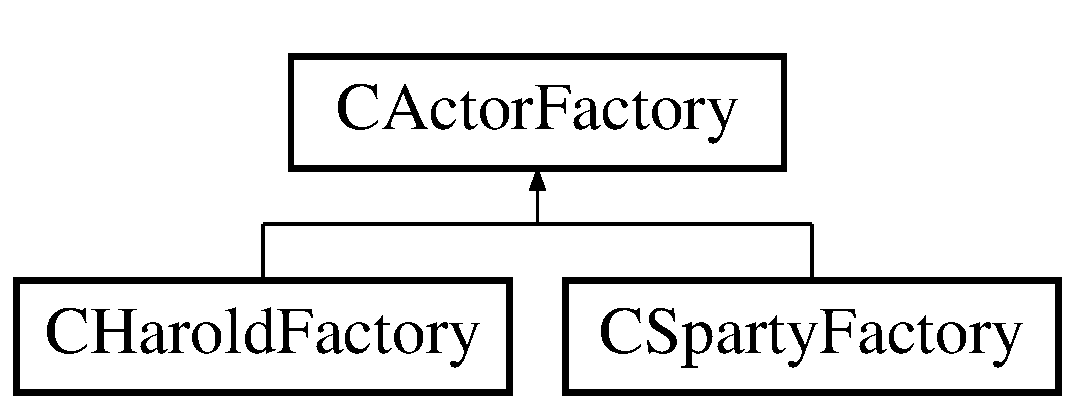
\includegraphics[height=2.000000cm]{class_c_actor_factory}
\end{center}
\end{figure}
\subsection*{Public Member Functions}
\begin{DoxyCompactItemize}
\item 
\hypertarget{class_c_actor_factory_a2c3174c6ca0362dbd3dbd2f599a51c46}{virtual \hyperlink{class_c_actor_factory_a2c3174c6ca0362dbd3dbd2f599a51c46}{$\sim$\+C\+Actor\+Factory} ()}\label{class_c_actor_factory_a2c3174c6ca0362dbd3dbd2f599a51c46}

\begin{DoxyCompactList}\small\item\em Destructor. \end{DoxyCompactList}\item 
virtual std\+::shared\+\_\+ptr$<$ \hyperlink{class_c_actor}{C\+Actor} $>$ \hyperlink{class_c_actor_factory_a1e751d97cc015ab2182b7683133e5a5d}{Create} ()=0
\begin{DoxyCompactList}\small\item\em Create the actor. \end{DoxyCompactList}\end{DoxyCompactItemize}
\subsection*{Protected Member Functions}
\begin{DoxyCompactItemize}
\item 
\hypertarget{class_c_actor_factory_a6a9d84ffa74ef0b01bf1e31fb28efcaa}{\hyperlink{class_c_actor_factory_a6a9d84ffa74ef0b01bf1e31fb28efcaa}{C\+Actor\+Factory} ()}\label{class_c_actor_factory_a6a9d84ffa74ef0b01bf1e31fb28efcaa}

\begin{DoxyCompactList}\small\item\em Constructor. \end{DoxyCompactList}\end{DoxyCompactItemize}


\subsection{Detailed Description}
Abstract base class for actor factories. 

\subsection{Member Function Documentation}
\hypertarget{class_c_actor_factory_a1e751d97cc015ab2182b7683133e5a5d}{\index{C\+Actor\+Factory@{C\+Actor\+Factory}!Create@{Create}}
\index{Create@{Create}!C\+Actor\+Factory@{C\+Actor\+Factory}}
\subsubsection[{Create}]{\setlength{\rightskip}{0pt plus 5cm}virtual std\+::shared\+\_\+ptr$<${\bf C\+Actor}$>$ C\+Actor\+Factory\+::\+Create (
\begin{DoxyParamCaption}
{}
\end{DoxyParamCaption}
)\hspace{0.3cm}{\ttfamily [pure virtual]}}}\label{class_c_actor_factory_a1e751d97cc015ab2182b7683133e5a5d}


Create the actor. 

\begin{DoxyReturn}{Returns}
New actor object 
\end{DoxyReturn}


Implemented in \hyperlink{class_c_sparty_factory_a171c122e80006b4adcc13a9e81faf3fc}{C\+Sparty\+Factory}, and \hyperlink{class_c_harold_factory_a785f8194f83d866bfc2a237fc3d4abc1}{C\+Harold\+Factory}.



The documentation for this class was generated from the following files\+:\begin{DoxyCompactItemize}
\item 
\hyperlink{_actor_factory_8h}{Actor\+Factory.\+h}\item 
\hyperlink{_actor_factory_8cpp}{Actor\+Factory.\+cpp}\end{DoxyCompactItemize}

\hypertarget{class_c_anim_channel}{\section{C\+Anim\+Channel Class Reference}
\label{class_c_anim_channel}\index{C\+Anim\+Channel@{C\+Anim\+Channel}}
}


Base class for an animation channel.  




{\ttfamily \#include $<$Anim\+Channel.\+h$>$}

Inheritance diagram for C\+Anim\+Channel\+:\begin{figure}[H]
\begin{center}
\leavevmode
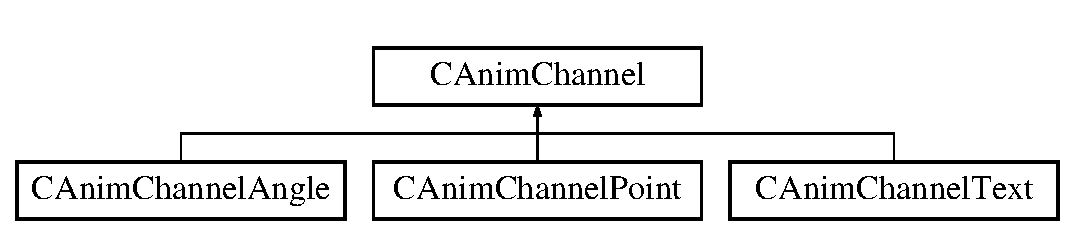
\includegraphics[height=2.000000cm]{class_c_anim_channel}
\end{center}
\end{figure}
\subsection*{Classes}
\begin{DoxyCompactItemize}
\item 
class \hyperlink{class_c_anim_channel_1_1_keyframe}{Keyframe}
\begin{DoxyCompactList}\small\item\em Class that represents a keyframe. \end{DoxyCompactList}\end{DoxyCompactItemize}
\subsection*{Public Member Functions}
\begin{DoxyCompactItemize}
\item 
\hypertarget{class_c_anim_channel_a1ce8a3d902476227d112459b662e2a4f}{\hyperlink{class_c_anim_channel_a1ce8a3d902476227d112459b662e2a4f}{C\+Anim\+Channel} ()}\label{class_c_anim_channel_a1ce8a3d902476227d112459b662e2a4f}

\begin{DoxyCompactList}\small\item\em Constructor. \end{DoxyCompactList}\item 
\hypertarget{class_c_anim_channel_a63a09f6e3f729b16130405f865c8f267}{virtual \hyperlink{class_c_anim_channel_a63a09f6e3f729b16130405f865c8f267}{$\sim$\+C\+Anim\+Channel} ()}\label{class_c_anim_channel_a63a09f6e3f729b16130405f865c8f267}

\begin{DoxyCompactList}\small\item\em Destructor. \end{DoxyCompactList}\item 
\hypertarget{class_c_anim_channel_aeb50ddc731a16230beef39cf198b78f9}{\hyperlink{class_c_anim_channel_aeb50ddc731a16230beef39cf198b78f9}{C\+Anim\+Channel} (const \hyperlink{class_c_anim_channel}{C\+Anim\+Channel} \&)=delete}\label{class_c_anim_channel_aeb50ddc731a16230beef39cf198b78f9}

\begin{DoxyCompactList}\small\item\em Copy constructor disabled. \end{DoxyCompactList}\item 
\hypertarget{class_c_anim_channel_a29ee3e3b8f1edf5947c08a6aad1d5bcd}{void \hyperlink{class_c_anim_channel_a29ee3e3b8f1edf5947c08a6aad1d5bcd}{operator=} (const \hyperlink{class_c_anim_channel}{C\+Anim\+Channel} \&)=delete}\label{class_c_anim_channel_a29ee3e3b8f1edf5947c08a6aad1d5bcd}

\begin{DoxyCompactList}\small\item\em Assignment operator disabled. \end{DoxyCompactList}\item 
void \hyperlink{class_c_anim_channel_acd94fef3b6bb9279aac24fd912198d47}{Set\+Name} (const std\+::wstring \&name)
\begin{DoxyCompactList}\small\item\em Set the channel name. \end{DoxyCompactList}\item 
std\+::wstring \hyperlink{class_c_anim_channel_a5719b94bb069345636f3b6274522bd0c}{Get\+Name} () const 
\begin{DoxyCompactList}\small\item\em Get the channel name. \end{DoxyCompactList}\item 
void \hyperlink{class_c_anim_channel_a73cb35e7bd3840e918a1762650541cab}{Set\+Timeline} (\hyperlink{class_c_timeline}{C\+Timeline} $\ast$timeline)
\begin{DoxyCompactList}\small\item\em Set the timeline for this channel. \end{DoxyCompactList}\item 
\hyperlink{class_c_timeline}{C\+Timeline} $\ast$ \hyperlink{class_c_anim_channel_a668a7b1770bb3f2605e937b905bcfde7}{Get\+Timeline} ()
\begin{DoxyCompactList}\small\item\em Get the timeline for this channel. \end{DoxyCompactList}\item 
void \hyperlink{class_c_anim_channel_a1f68764b84b12c943570cfd2e08d7015}{Set\+Frame} (int curr\+Frame)
\begin{DoxyCompactList}\small\item\em Ensure the keyframe indices are valid for the current time. \end{DoxyCompactList}\item 
bool \hyperlink{class_c_anim_channel_ada18e6cdd72a834417b1067be1205a3f}{Is\+Valid} ()
\begin{DoxyCompactList}\small\item\em Is the channel valid, meaning has keyframes? \end{DoxyCompactList}\item 
\hypertarget{class_c_anim_channel_abccfa21587f36a2edb9365ce986a21e2}{void \hyperlink{class_c_anim_channel_abccfa21587f36a2edb9365ce986a21e2}{Clear\+Keyframe} ()}\label{class_c_anim_channel_abccfa21587f36a2edb9365ce986a21e2}

\begin{DoxyCompactList}\small\item\em Clear the current keyframe. \end{DoxyCompactList}\item 
virtual std\+::shared\+\_\+ptr\\*
$<$ \hyperlink{classxmlnode_1_1_c_xml_node}{xmlnode\+::\+C\+Xml\+Node} $>$ \hyperlink{class_c_anim_channel_ad4b87256e49f954eaf1dbcfa54fba34a}{Xml\+Save} (const std\+::shared\+\_\+ptr$<$ \hyperlink{classxmlnode_1_1_c_xml_node}{xmlnode\+::\+C\+Xml\+Node} $>$ \&node)
\begin{DoxyCompactList}\small\item\em Save this item to an X\+M\+L node. \end{DoxyCompactList}\item 
\hypertarget{class_c_anim_channel_ae9b7297011e630f9e621fee0dcac3a75}{virtual void \hyperlink{class_c_anim_channel_ae9b7297011e630f9e621fee0dcac3a75}{Clear} ()}\label{class_c_anim_channel_ae9b7297011e630f9e621fee0dcac3a75}

\begin{DoxyCompactList}\small\item\em Clear all keyframes for this channel. \end{DoxyCompactList}\item 
virtual void \hyperlink{class_c_anim_channel_a93a846ae42defd51e172ca922dfee742}{Xml\+Load} (const std\+::shared\+\_\+ptr$<$ \hyperlink{classxmlnode_1_1_c_xml_node}{xmlnode\+::\+C\+Xml\+Node} $>$ \&node)
\begin{DoxyCompactList}\small\item\em Handle loading this channel from a channel tag. \end{DoxyCompactList}\end{DoxyCompactItemize}
\subsection*{Protected Member Functions}
\begin{DoxyCompactItemize}
\item 
void \hyperlink{class_c_anim_channel_a8c29b90a984072bce8cf2f8ea03d0e5b}{Insert\+Keyframe} (std\+::shared\+\_\+ptr$<$ \hyperlink{class_c_anim_channel_1_1_keyframe}{Keyframe} $>$ keyframe)
\begin{DoxyCompactList}\small\item\em Determine how we should insert a keyframe into our keyframe list. \end{DoxyCompactList}\item 
virtual void \hyperlink{class_c_anim_channel_a2df7b3fed2b3faf34c585446628fc874}{Xml\+Load\+Keyframe} (const std\+::shared\+\_\+ptr$<$ \hyperlink{classxmlnode_1_1_c_xml_node}{xmlnode\+::\+C\+Xml\+Node} $>$ \&node)=0
\begin{DoxyCompactList}\small\item\em Channel type specific loading and keyframe creation. \end{DoxyCompactList}\item 
virtual void \hyperlink{class_c_anim_channel_adf83febfff4c3db9e9f56de72735f8ee}{Tween} (double t)=0
\begin{DoxyCompactList}\small\item\em Tween between two keyframes. \end{DoxyCompactList}\end{DoxyCompactItemize}


\subsection{Detailed Description}
Base class for an animation channel. 

\subsection{Member Function Documentation}
\hypertarget{class_c_anim_channel_a5719b94bb069345636f3b6274522bd0c}{\index{C\+Anim\+Channel@{C\+Anim\+Channel}!Get\+Name@{Get\+Name}}
\index{Get\+Name@{Get\+Name}!C\+Anim\+Channel@{C\+Anim\+Channel}}
\subsubsection[{Get\+Name}]{\setlength{\rightskip}{0pt plus 5cm}std\+::wstring C\+Anim\+Channel\+::\+Get\+Name (
\begin{DoxyParamCaption}
{}
\end{DoxyParamCaption}
) const\hspace{0.3cm}{\ttfamily [inline]}}}\label{class_c_anim_channel_a5719b94bb069345636f3b6274522bd0c}


Get the channel name. 

\begin{DoxyReturn}{Returns}
Channel name 
\end{DoxyReturn}
\hypertarget{class_c_anim_channel_a668a7b1770bb3f2605e937b905bcfde7}{\index{C\+Anim\+Channel@{C\+Anim\+Channel}!Get\+Timeline@{Get\+Timeline}}
\index{Get\+Timeline@{Get\+Timeline}!C\+Anim\+Channel@{C\+Anim\+Channel}}
\subsubsection[{Get\+Timeline}]{\setlength{\rightskip}{0pt plus 5cm}{\bf C\+Timeline}$\ast$ C\+Anim\+Channel\+::\+Get\+Timeline (
\begin{DoxyParamCaption}
{}
\end{DoxyParamCaption}
)\hspace{0.3cm}{\ttfamily [inline]}}}\label{class_c_anim_channel_a668a7b1770bb3f2605e937b905bcfde7}


Get the timeline for this channel. 

\begin{DoxyReturn}{Returns}
The timeline pointer 
\end{DoxyReturn}
\hypertarget{class_c_anim_channel_a8c29b90a984072bce8cf2f8ea03d0e5b}{\index{C\+Anim\+Channel@{C\+Anim\+Channel}!Insert\+Keyframe@{Insert\+Keyframe}}
\index{Insert\+Keyframe@{Insert\+Keyframe}!C\+Anim\+Channel@{C\+Anim\+Channel}}
\subsubsection[{Insert\+Keyframe}]{\setlength{\rightskip}{0pt plus 5cm}void C\+Anim\+Channel\+::\+Insert\+Keyframe (
\begin{DoxyParamCaption}
\item[{std\+::shared\+\_\+ptr$<$ {\bf Keyframe} $>$}]{keyframe}
\end{DoxyParamCaption}
)\hspace{0.3cm}{\ttfamily [protected]}}}\label{class_c_anim_channel_a8c29b90a984072bce8cf2f8ea03d0e5b}


Determine how we should insert a keyframe into our keyframe list. 


\begin{DoxyParams}{Parameters}
{\em keyframe} & The keyframe to insert \\
\hline
\end{DoxyParams}
\hypertarget{class_c_anim_channel_ada18e6cdd72a834417b1067be1205a3f}{\index{C\+Anim\+Channel@{C\+Anim\+Channel}!Is\+Valid@{Is\+Valid}}
\index{Is\+Valid@{Is\+Valid}!C\+Anim\+Channel@{C\+Anim\+Channel}}
\subsubsection[{Is\+Valid}]{\setlength{\rightskip}{0pt plus 5cm}bool C\+Anim\+Channel\+::\+Is\+Valid (
\begin{DoxyParamCaption}
{}
\end{DoxyParamCaption}
)\hspace{0.3cm}{\ttfamily [inline]}}}\label{class_c_anim_channel_ada18e6cdd72a834417b1067be1205a3f}


Is the channel valid, meaning has keyframes? 

\begin{DoxyReturn}{Returns}
true if the channel is valid. 
\end{DoxyReturn}
\hypertarget{class_c_anim_channel_a1f68764b84b12c943570cfd2e08d7015}{\index{C\+Anim\+Channel@{C\+Anim\+Channel}!Set\+Frame@{Set\+Frame}}
\index{Set\+Frame@{Set\+Frame}!C\+Anim\+Channel@{C\+Anim\+Channel}}
\subsubsection[{Set\+Frame}]{\setlength{\rightskip}{0pt plus 5cm}void C\+Anim\+Channel\+::\+Set\+Frame (
\begin{DoxyParamCaption}
\item[{int}]{curr\+Frame}
\end{DoxyParamCaption}
)}}\label{class_c_anim_channel_a1f68764b84b12c943570cfd2e08d7015}


Ensure the keyframe indices are valid for the current time. 

The location pointed to by keyframe1 must be a time less than or equal to the current time and the location pointed to by keyframe2 must be the next location and a location greater than the current time. Note that the time may be before or after the first or last item in the list. We indicate that with values of -\/1 for the indices. 
\begin{DoxyParams}{Parameters}
{\em curr\+Frame} & The frame we are on. \\
\hline
\end{DoxyParams}
\hypertarget{class_c_anim_channel_acd94fef3b6bb9279aac24fd912198d47}{\index{C\+Anim\+Channel@{C\+Anim\+Channel}!Set\+Name@{Set\+Name}}
\index{Set\+Name@{Set\+Name}!C\+Anim\+Channel@{C\+Anim\+Channel}}
\subsubsection[{Set\+Name}]{\setlength{\rightskip}{0pt plus 5cm}void C\+Anim\+Channel\+::\+Set\+Name (
\begin{DoxyParamCaption}
\item[{const std\+::wstring \&}]{name}
\end{DoxyParamCaption}
)\hspace{0.3cm}{\ttfamily [inline]}}}\label{class_c_anim_channel_acd94fef3b6bb9279aac24fd912198d47}


Set the channel name. 


\begin{DoxyParams}{Parameters}
{\em name} & The new name to set \\
\hline
\end{DoxyParams}
\hypertarget{class_c_anim_channel_a73cb35e7bd3840e918a1762650541cab}{\index{C\+Anim\+Channel@{C\+Anim\+Channel}!Set\+Timeline@{Set\+Timeline}}
\index{Set\+Timeline@{Set\+Timeline}!C\+Anim\+Channel@{C\+Anim\+Channel}}
\subsubsection[{Set\+Timeline}]{\setlength{\rightskip}{0pt plus 5cm}void C\+Anim\+Channel\+::\+Set\+Timeline (
\begin{DoxyParamCaption}
\item[{{\bf C\+Timeline} $\ast$}]{timeline}
\end{DoxyParamCaption}
)\hspace{0.3cm}{\ttfamily [inline]}}}\label{class_c_anim_channel_a73cb35e7bd3840e918a1762650541cab}


Set the timeline for this channel. 


\begin{DoxyParams}{Parameters}
{\em timeline} & The timeline to use \\
\hline
\end{DoxyParams}
\hypertarget{class_c_anim_channel_adf83febfff4c3db9e9f56de72735f8ee}{\index{C\+Anim\+Channel@{C\+Anim\+Channel}!Tween@{Tween}}
\index{Tween@{Tween}!C\+Anim\+Channel@{C\+Anim\+Channel}}
\subsubsection[{Tween}]{\setlength{\rightskip}{0pt plus 5cm}virtual void C\+Anim\+Channel\+::\+Tween (
\begin{DoxyParamCaption}
\item[{double}]{t}
\end{DoxyParamCaption}
)\hspace{0.3cm}{\ttfamily [protected]}, {\ttfamily [pure virtual]}}}\label{class_c_anim_channel_adf83febfff4c3db9e9f56de72735f8ee}


Tween between two keyframes. 


\begin{DoxyParams}{Parameters}
{\em t} & The T value (0 to 1) \\
\hline
\end{DoxyParams}


Implemented in \hyperlink{class_c_anim_channel_text_a6bf49ec2ab6856c8741999e64031f99f}{C\+Anim\+Channel\+Text}, \hyperlink{class_c_anim_channel_angle_a2fe6ecc9f2cc1629efa18c33d2742e4d}{C\+Anim\+Channel\+Angle}, and \hyperlink{class_c_anim_channel_point_ac67b18d31453f8e25c681423c3e056c8}{C\+Anim\+Channel\+Point}.

\hypertarget{class_c_anim_channel_a93a846ae42defd51e172ca922dfee742}{\index{C\+Anim\+Channel@{C\+Anim\+Channel}!Xml\+Load@{Xml\+Load}}
\index{Xml\+Load@{Xml\+Load}!C\+Anim\+Channel@{C\+Anim\+Channel}}
\subsubsection[{Xml\+Load}]{\setlength{\rightskip}{0pt plus 5cm}void C\+Anim\+Channel\+::\+Xml\+Load (
\begin{DoxyParamCaption}
\item[{const std\+::shared\+\_\+ptr$<$ {\bf xmlnode\+::\+C\+Xml\+Node} $>$ \&}]{node}
\end{DoxyParamCaption}
)\hspace{0.3cm}{\ttfamily [virtual]}}}\label{class_c_anim_channel_a93a846ae42defd51e172ca922dfee742}


Handle loading this channel from a channel tag. 


\begin{DoxyParams}{Parameters}
{\em node} & channel tag node \\
\hline
\end{DoxyParams}
\hypertarget{class_c_anim_channel_a2df7b3fed2b3faf34c585446628fc874}{\index{C\+Anim\+Channel@{C\+Anim\+Channel}!Xml\+Load\+Keyframe@{Xml\+Load\+Keyframe}}
\index{Xml\+Load\+Keyframe@{Xml\+Load\+Keyframe}!C\+Anim\+Channel@{C\+Anim\+Channel}}
\subsubsection[{Xml\+Load\+Keyframe}]{\setlength{\rightskip}{0pt plus 5cm}virtual void C\+Anim\+Channel\+::\+Xml\+Load\+Keyframe (
\begin{DoxyParamCaption}
\item[{const std\+::shared\+\_\+ptr$<$ {\bf xmlnode\+::\+C\+Xml\+Node} $>$ \&}]{node}
\end{DoxyParamCaption}
)\hspace{0.3cm}{\ttfamily [protected]}, {\ttfamily [pure virtual]}}}\label{class_c_anim_channel_a2df7b3fed2b3faf34c585446628fc874}


Channel type specific loading and keyframe creation. 


\begin{DoxyParams}{Parameters}
{\em node} & Node to load from \\
\hline
\end{DoxyParams}


Implemented in \hyperlink{class_c_anim_channel_text_af30a93b795d45ad49c498c0e96313afd}{C\+Anim\+Channel\+Text}, \hyperlink{class_c_anim_channel_angle_a7c56ed07ead2eab289e07dbd39c1bf90}{C\+Anim\+Channel\+Angle}, and \hyperlink{class_c_anim_channel_point_a7eb61594e08c2f0177f086bc3af9221f}{C\+Anim\+Channel\+Point}.

\hypertarget{class_c_anim_channel_ad4b87256e49f954eaf1dbcfa54fba34a}{\index{C\+Anim\+Channel@{C\+Anim\+Channel}!Xml\+Save@{Xml\+Save}}
\index{Xml\+Save@{Xml\+Save}!C\+Anim\+Channel@{C\+Anim\+Channel}}
\subsubsection[{Xml\+Save}]{\setlength{\rightskip}{0pt plus 5cm}std\+::shared\+\_\+ptr$<$ {\bf xmlnode\+::\+C\+Xml\+Node} $>$ C\+Anim\+Channel\+::\+Xml\+Save (
\begin{DoxyParamCaption}
\item[{const std\+::shared\+\_\+ptr$<$ {\bf xmlnode\+::\+C\+Xml\+Node} $>$ \&}]{node}
\end{DoxyParamCaption}
)\hspace{0.3cm}{\ttfamily [virtual]}}}\label{class_c_anim_channel_ad4b87256e49f954eaf1dbcfa54fba34a}


Save this item to an X\+M\+L node. 


\begin{DoxyParams}{Parameters}
{\em node} & The node we are going to be a child of \\
\hline
\end{DoxyParams}
\begin{DoxyReturn}{Returns}
Allocated X\+M\+L node. 
\end{DoxyReturn}


The documentation for this class was generated from the following files\+:\begin{DoxyCompactItemize}
\item 
\hyperlink{_anim_channel_8h}{Anim\+Channel.\+h}\item 
\hyperlink{_anim_channel_8cpp}{Anim\+Channel.\+cpp}\end{DoxyCompactItemize}

\hypertarget{class_c_anim_channel_angle}{\section{C\+Anim\+Channel\+Angle Class Reference}
\label{class_c_anim_channel_angle}\index{C\+Anim\+Channel\+Angle@{C\+Anim\+Channel\+Angle}}
}


Animation channel for angles.  




{\ttfamily \#include $<$Anim\+Channel\+Angle.\+h$>$}

Inheritance diagram for C\+Anim\+Channel\+Angle\+:\begin{figure}[H]
\begin{center}
\leavevmode
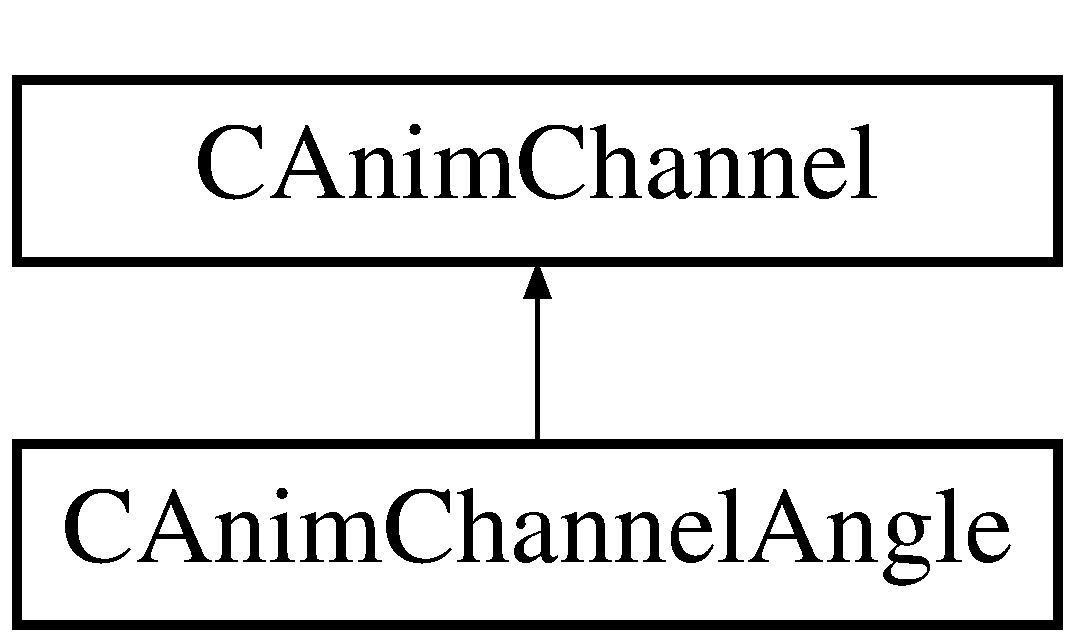
\includegraphics[height=2.000000cm]{class_c_anim_channel_angle}
\end{center}
\end{figure}
\subsection*{Classes}
\begin{DoxyCompactItemize}
\item 
class \hyperlink{class_c_anim_channel_angle_1_1_keyframe_angle}{Keyframe\+Angle}
\begin{DoxyCompactList}\small\item\em A keyframe for an angle channel. \end{DoxyCompactList}\end{DoxyCompactItemize}
\subsection*{Public Member Functions}
\begin{DoxyCompactItemize}
\item 
\hypertarget{class_c_anim_channel_angle_a408925f5093ef5bca8bcebc2917fe577}{\hyperlink{class_c_anim_channel_angle_a408925f5093ef5bca8bcebc2917fe577}{C\+Anim\+Channel\+Angle} ()}\label{class_c_anim_channel_angle_a408925f5093ef5bca8bcebc2917fe577}

\begin{DoxyCompactList}\small\item\em Constructor. \end{DoxyCompactList}\item 
\hypertarget{class_c_anim_channel_angle_aa6fd09295d3868da87a06b4173fdc955}{virtual \hyperlink{class_c_anim_channel_angle_aa6fd09295d3868da87a06b4173fdc955}{$\sim$\+C\+Anim\+Channel\+Angle} ()}\label{class_c_anim_channel_angle_aa6fd09295d3868da87a06b4173fdc955}

\begin{DoxyCompactList}\small\item\em Destructor. \end{DoxyCompactList}\item 
double \hyperlink{class_c_anim_channel_angle_a0fda0dabc9e7d7a44760b75aab85abf4}{Get\+Angle} ()
\begin{DoxyCompactList}\small\item\em Get the current time angle. \end{DoxyCompactList}\item 
void \hyperlink{class_c_anim_channel_angle_a20bb427cc1a790d1449f770ac413dc95}{Set\+Keyframe} (double angle)
\begin{DoxyCompactList}\small\item\em Set a keyframe. \end{DoxyCompactList}\item 
void \hyperlink{class_c_anim_channel_angle_a2fe6ecc9f2cc1629efa18c33d2742e4d}{Tween} (double t)
\begin{DoxyCompactList}\small\item\em Tween between two angle keyframes. \end{DoxyCompactList}\end{DoxyCompactItemize}
\subsection*{Protected Member Functions}
\begin{DoxyCompactItemize}
\item 
virtual void \hyperlink{class_c_anim_channel_angle_a7c56ed07ead2eab289e07dbd39c1bf90}{Xml\+Load\+Keyframe} (const std\+::shared\+\_\+ptr$<$ \hyperlink{classxmlnode_1_1_c_xml_node}{xmlnode\+::\+C\+Xml\+Node} $>$ \&node) override
\begin{DoxyCompactList}\small\item\em Handle loading this channel's keyframe type. \end{DoxyCompactList}\end{DoxyCompactItemize}


\subsection{Detailed Description}
Animation channel for angles. 

\subsection{Member Function Documentation}
\hypertarget{class_c_anim_channel_angle_a0fda0dabc9e7d7a44760b75aab85abf4}{\index{C\+Anim\+Channel\+Angle@{C\+Anim\+Channel\+Angle}!Get\+Angle@{Get\+Angle}}
\index{Get\+Angle@{Get\+Angle}!C\+Anim\+Channel\+Angle@{C\+Anim\+Channel\+Angle}}
\subsubsection[{Get\+Angle}]{\setlength{\rightskip}{0pt plus 5cm}double C\+Anim\+Channel\+Angle\+::\+Get\+Angle (
\begin{DoxyParamCaption}
{}
\end{DoxyParamCaption}
)\hspace{0.3cm}{\ttfamily [inline]}}}\label{class_c_anim_channel_angle_a0fda0dabc9e7d7a44760b75aab85abf4}


Get the current time angle. 

\begin{DoxyReturn}{Returns}
Angle in radians 
\end{DoxyReturn}
\hypertarget{class_c_anim_channel_angle_a20bb427cc1a790d1449f770ac413dc95}{\index{C\+Anim\+Channel\+Angle@{C\+Anim\+Channel\+Angle}!Set\+Keyframe@{Set\+Keyframe}}
\index{Set\+Keyframe@{Set\+Keyframe}!C\+Anim\+Channel\+Angle@{C\+Anim\+Channel\+Angle}}
\subsubsection[{Set\+Keyframe}]{\setlength{\rightskip}{0pt plus 5cm}void C\+Anim\+Channel\+Angle\+::\+Set\+Keyframe (
\begin{DoxyParamCaption}
\item[{double}]{angle}
\end{DoxyParamCaption}
)}}\label{class_c_anim_channel_angle_a20bb427cc1a790d1449f770ac413dc95}


Set a keyframe. 

This function allocates a new keyframe and sends it to \hyperlink{class_c_anim_channel}{C\+Anim\+Channel}, which will insert it into the collection of keyframes. 
\begin{DoxyParams}{Parameters}
{\em angle} & Angle for the keyframe. \\
\hline
\end{DoxyParams}
\hypertarget{class_c_anim_channel_angle_a2fe6ecc9f2cc1629efa18c33d2742e4d}{\index{C\+Anim\+Channel\+Angle@{C\+Anim\+Channel\+Angle}!Tween@{Tween}}
\index{Tween@{Tween}!C\+Anim\+Channel\+Angle@{C\+Anim\+Channel\+Angle}}
\subsubsection[{Tween}]{\setlength{\rightskip}{0pt plus 5cm}void C\+Anim\+Channel\+Angle\+::\+Tween (
\begin{DoxyParamCaption}
\item[{double}]{t}
\end{DoxyParamCaption}
)\hspace{0.3cm}{\ttfamily [virtual]}}}\label{class_c_anim_channel_angle_a2fe6ecc9f2cc1629efa18c33d2742e4d}


Tween between two angle keyframes. 


\begin{DoxyParams}{Parameters}
{\em t} & The t value between the frames \\
\hline
\end{DoxyParams}


Implements \hyperlink{class_c_anim_channel_adf83febfff4c3db9e9f56de72735f8ee}{C\+Anim\+Channel}.

\hypertarget{class_c_anim_channel_angle_a7c56ed07ead2eab289e07dbd39c1bf90}{\index{C\+Anim\+Channel\+Angle@{C\+Anim\+Channel\+Angle}!Xml\+Load\+Keyframe@{Xml\+Load\+Keyframe}}
\index{Xml\+Load\+Keyframe@{Xml\+Load\+Keyframe}!C\+Anim\+Channel\+Angle@{C\+Anim\+Channel\+Angle}}
\subsubsection[{Xml\+Load\+Keyframe}]{\setlength{\rightskip}{0pt plus 5cm}void C\+Anim\+Channel\+Angle\+::\+Xml\+Load\+Keyframe (
\begin{DoxyParamCaption}
\item[{const std\+::shared\+\_\+ptr$<$ {\bf xmlnode\+::\+C\+Xml\+Node} $>$ \&}]{node}
\end{DoxyParamCaption}
)\hspace{0.3cm}{\ttfamily [override]}, {\ttfamily [protected]}, {\ttfamily [virtual]}}}\label{class_c_anim_channel_angle_a7c56ed07ead2eab289e07dbd39c1bf90}


Handle loading this channel's keyframe type. 


\begin{DoxyParams}{Parameters}
{\em node} & keyframe tag node \\
\hline
\end{DoxyParams}


Implements \hyperlink{class_c_anim_channel_a2df7b3fed2b3faf34c585446628fc874}{C\+Anim\+Channel}.



The documentation for this class was generated from the following files\+:\begin{DoxyCompactItemize}
\item 
\hyperlink{_anim_channel_angle_8h}{Anim\+Channel\+Angle.\+h}\item 
\hyperlink{_anim_channel_angle_8cpp}{Anim\+Channel\+Angle.\+cpp}\end{DoxyCompactItemize}

\hypertarget{class_c_anim_channel_point}{\section{C\+Anim\+Channel\+Point Class Reference}
\label{class_c_anim_channel_point}\index{C\+Anim\+Channel\+Point@{C\+Anim\+Channel\+Point}}
}


An animation channel specific to points (movement)  




{\ttfamily \#include $<$Anim\+Channel\+Point.\+h$>$}

Inheritance diagram for C\+Anim\+Channel\+Point\+:\begin{figure}[H]
\begin{center}
\leavevmode
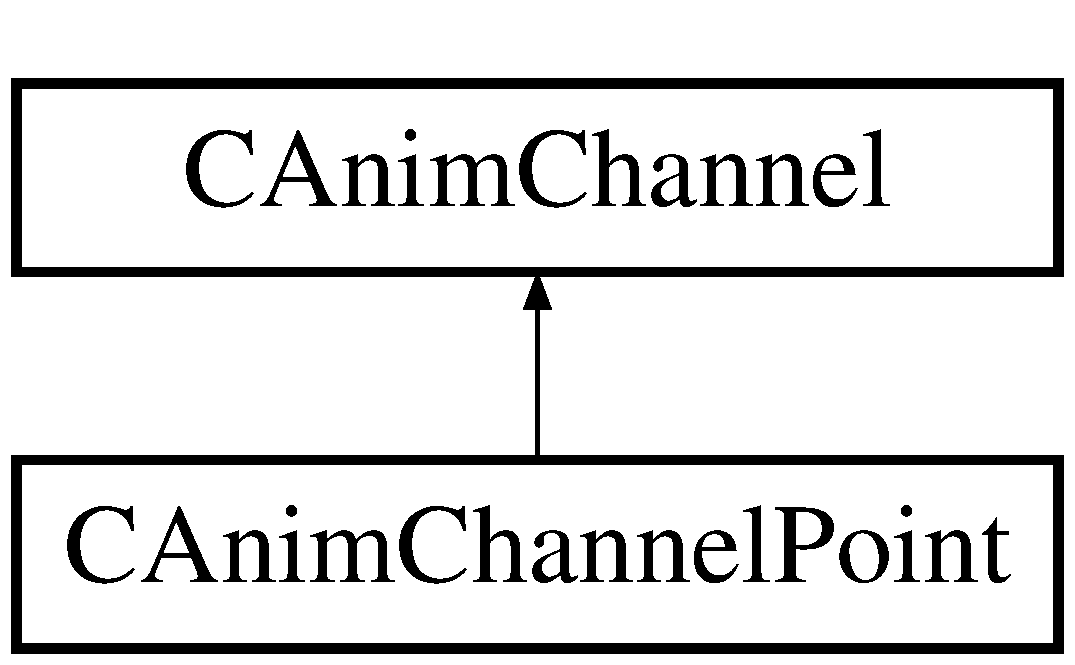
\includegraphics[height=2.000000cm]{class_c_anim_channel_point}
\end{center}
\end{figure}
\subsection*{Classes}
\begin{DoxyCompactItemize}
\item 
class \hyperlink{class_c_anim_channel_point_1_1_keyframe_point}{Keyframe\+Point}
\begin{DoxyCompactList}\small\item\em A keyframe for a point channel. \end{DoxyCompactList}\end{DoxyCompactItemize}
\subsection*{Public Member Functions}
\begin{DoxyCompactItemize}
\item 
\hypertarget{class_c_anim_channel_point_ac887ebf37797918e29197cd855eb3d60}{\hyperlink{class_c_anim_channel_point_ac887ebf37797918e29197cd855eb3d60}{C\+Anim\+Channel\+Point} ()}\label{class_c_anim_channel_point_ac887ebf37797918e29197cd855eb3d60}

\begin{DoxyCompactList}\small\item\em Constructor. \end{DoxyCompactList}\item 
\hypertarget{class_c_anim_channel_point_ac0ffdb24903c2ae673686d53b2e1dadb}{\hyperlink{class_c_anim_channel_point_ac0ffdb24903c2ae673686d53b2e1dadb}{$\sim$\+C\+Anim\+Channel\+Point} ()}\label{class_c_anim_channel_point_ac0ffdb24903c2ae673686d53b2e1dadb}

\begin{DoxyCompactList}\small\item\em Destructor. \end{DoxyCompactList}\item 
Gdiplus\+::\+Point \hyperlink{class_c_anim_channel_point_a8885cd8eb06b4af6d9997e7d79c1d856}{Get\+Point} ()
\begin{DoxyCompactList}\small\item\em The point we compute. \end{DoxyCompactList}\item 
void \hyperlink{class_c_anim_channel_point_abcfdddd770020c17e5736ccf6bb15912}{Set\+Keyframe} (Gdiplus\+::\+Point point)
\begin{DoxyCompactList}\small\item\em Set a keyframe. \end{DoxyCompactList}\item 
void \hyperlink{class_c_anim_channel_point_ac67b18d31453f8e25c681423c3e056c8}{Tween} (double t)
\begin{DoxyCompactList}\small\item\em Compute a tweened point between to points. \end{DoxyCompactList}\end{DoxyCompactItemize}
\subsection*{Protected Member Functions}
\begin{DoxyCompactItemize}
\item 
virtual void \hyperlink{class_c_anim_channel_point_a7eb61594e08c2f0177f086bc3af9221f}{Xml\+Load\+Keyframe} (const std\+::shared\+\_\+ptr$<$ \hyperlink{classxmlnode_1_1_c_xml_node}{xmlnode\+::\+C\+Xml\+Node} $>$ \&node) override
\begin{DoxyCompactList}\small\item\em Handle loading this channel's keyframe type. \end{DoxyCompactList}\end{DoxyCompactItemize}


\subsection{Detailed Description}
An animation channel specific to points (movement) 

\subsection{Member Function Documentation}
\hypertarget{class_c_anim_channel_point_a8885cd8eb06b4af6d9997e7d79c1d856}{\index{C\+Anim\+Channel\+Point@{C\+Anim\+Channel\+Point}!Get\+Point@{Get\+Point}}
\index{Get\+Point@{Get\+Point}!C\+Anim\+Channel\+Point@{C\+Anim\+Channel\+Point}}
\subsubsection[{Get\+Point}]{\setlength{\rightskip}{0pt plus 5cm}Gdiplus\+::\+Point C\+Anim\+Channel\+Point\+::\+Get\+Point (
\begin{DoxyParamCaption}
{}
\end{DoxyParamCaption}
)\hspace{0.3cm}{\ttfamily [inline]}}}\label{class_c_anim_channel_point_a8885cd8eb06b4af6d9997e7d79c1d856}


The point we compute. 

\begin{DoxyReturn}{Returns}
The computed point 
\end{DoxyReturn}
\hypertarget{class_c_anim_channel_point_abcfdddd770020c17e5736ccf6bb15912}{\index{C\+Anim\+Channel\+Point@{C\+Anim\+Channel\+Point}!Set\+Keyframe@{Set\+Keyframe}}
\index{Set\+Keyframe@{Set\+Keyframe}!C\+Anim\+Channel\+Point@{C\+Anim\+Channel\+Point}}
\subsubsection[{Set\+Keyframe}]{\setlength{\rightskip}{0pt plus 5cm}void C\+Anim\+Channel\+Point\+::\+Set\+Keyframe (
\begin{DoxyParamCaption}
\item[{Gdiplus\+::\+Point}]{point}
\end{DoxyParamCaption}
)}}\label{class_c_anim_channel_point_abcfdddd770020c17e5736ccf6bb15912}


Set a keyframe. 

This function allocates a new keyframe and sends it to \hyperlink{class_c_anim_channel}{C\+Anim\+Channel}, which will insert it into the collection of keyframes. 
\begin{DoxyParams}{Parameters}
{\em point} & The point for the keyframe \\
\hline
\end{DoxyParams}
\hypertarget{class_c_anim_channel_point_ac67b18d31453f8e25c681423c3e056c8}{\index{C\+Anim\+Channel\+Point@{C\+Anim\+Channel\+Point}!Tween@{Tween}}
\index{Tween@{Tween}!C\+Anim\+Channel\+Point@{C\+Anim\+Channel\+Point}}
\subsubsection[{Tween}]{\setlength{\rightskip}{0pt plus 5cm}void C\+Anim\+Channel\+Point\+::\+Tween (
\begin{DoxyParamCaption}
\item[{double}]{t}
\end{DoxyParamCaption}
)\hspace{0.3cm}{\ttfamily [virtual]}}}\label{class_c_anim_channel_point_ac67b18d31453f8e25c681423c3e056c8}


Compute a tweened point between to points. 


\begin{DoxyParams}{Parameters}
{\em t} & The tweening t value \\
\hline
\end{DoxyParams}


Implements \hyperlink{class_c_anim_channel_adf83febfff4c3db9e9f56de72735f8ee}{C\+Anim\+Channel}.

\hypertarget{class_c_anim_channel_point_a7eb61594e08c2f0177f086bc3af9221f}{\index{C\+Anim\+Channel\+Point@{C\+Anim\+Channel\+Point}!Xml\+Load\+Keyframe@{Xml\+Load\+Keyframe}}
\index{Xml\+Load\+Keyframe@{Xml\+Load\+Keyframe}!C\+Anim\+Channel\+Point@{C\+Anim\+Channel\+Point}}
\subsubsection[{Xml\+Load\+Keyframe}]{\setlength{\rightskip}{0pt plus 5cm}void C\+Anim\+Channel\+Point\+::\+Xml\+Load\+Keyframe (
\begin{DoxyParamCaption}
\item[{const std\+::shared\+\_\+ptr$<$ {\bf xmlnode\+::\+C\+Xml\+Node} $>$ \&}]{node}
\end{DoxyParamCaption}
)\hspace{0.3cm}{\ttfamily [override]}, {\ttfamily [protected]}, {\ttfamily [virtual]}}}\label{class_c_anim_channel_point_a7eb61594e08c2f0177f086bc3af9221f}


Handle loading this channel's keyframe type. 


\begin{DoxyParams}{Parameters}
{\em node} & keyframe tag node \\
\hline
\end{DoxyParams}


Implements \hyperlink{class_c_anim_channel_a2df7b3fed2b3faf34c585446628fc874}{C\+Anim\+Channel}.



The documentation for this class was generated from the following files\+:\begin{DoxyCompactItemize}
\item 
\hyperlink{_anim_channel_point_8h}{Anim\+Channel\+Point.\+h}\item 
\hyperlink{_anim_channel_point_8cpp}{Anim\+Channel\+Point.\+cpp}\end{DoxyCompactItemize}

\hypertarget{class_c_anim_channel_text}{\section{C\+Anim\+Channel\+Text Class Reference}
\label{class_c_anim_channel_text}\index{C\+Anim\+Channel\+Text@{C\+Anim\+Channel\+Text}}
}
Inheritance diagram for C\+Anim\+Channel\+Text\+:\begin{figure}[H]
\begin{center}
\leavevmode
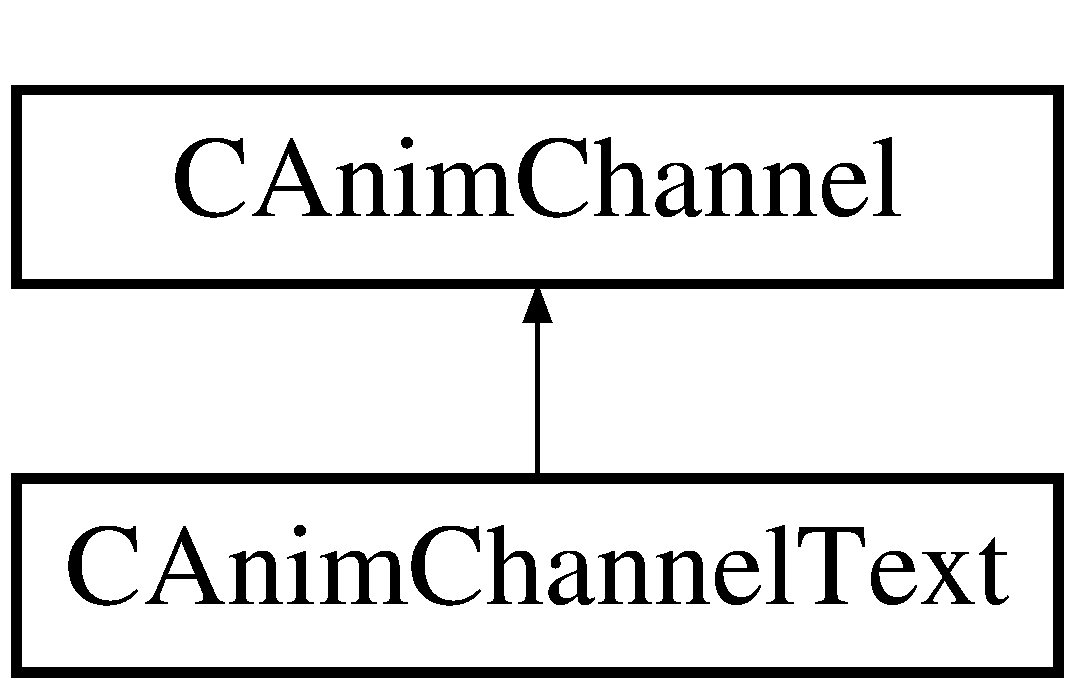
\includegraphics[height=2.000000cm]{class_c_anim_channel_text}
\end{center}
\end{figure}
\subsection*{Classes}
\begin{DoxyCompactItemize}
\item 
class \hyperlink{class_c_anim_channel_text_1_1_keyframe_text}{Keyframe\+Text}
\begin{DoxyCompactList}\small\item\em A ket frame for the text channel. \end{DoxyCompactList}\end{DoxyCompactItemize}
\subsection*{Public Member Functions}
\begin{DoxyCompactItemize}
\item 
\hypertarget{class_c_anim_channel_text_ae18bb8f72259762f55a3a66c19d89163}{std\+::wstring \hyperlink{class_c_anim_channel_text_ae18bb8f72259762f55a3a66c19d89163}{Get\+Text} ()}\label{class_c_anim_channel_text_ae18bb8f72259762f55a3a66c19d89163}

\begin{DoxyCompactList}\small\item\em Get the text in the channel. \end{DoxyCompactList}\item 
\hypertarget{class_c_anim_channel_text_afcba15848a3ab98d7e418b24a7bdbe40}{bool \hyperlink{class_c_anim_channel_text_afcba15848a3ab98d7e418b24a7bdbe40}{Get\+Mirror} ()}\label{class_c_anim_channel_text_afcba15848a3ab98d7e418b24a7bdbe40}

\begin{DoxyCompactList}\small\item\em Get if the text bubble is mirrored. \end{DoxyCompactList}\item 
void \hyperlink{class_c_anim_channel_text_a4defed1bebd5453add702bdee67b0dd8}{Set\+Keyframe} (std\+::wstring text, bool mirror)
\begin{DoxyCompactList}\small\item\em Set the keyframe with given text mirror value. \end{DoxyCompactList}\item 
virtual void \hyperlink{class_c_anim_channel_text_a6bf49ec2ab6856c8741999e64031f99f}{Tween} (double t) override
\begin{DoxyCompactList}\small\item\em set the text mirro value between two keyfreams \end{DoxyCompactList}\end{DoxyCompactItemize}
\subsection*{Protected Member Functions}
\begin{DoxyCompactItemize}
\item 
virtual void \hyperlink{class_c_anim_channel_text_af30a93b795d45ad49c498c0e96313afd}{Xml\+Load\+Keyframe} (const std\+::shared\+\_\+ptr$<$ \hyperlink{classxmlnode_1_1_c_xml_node}{xmlnode\+::\+C\+Xml\+Node} $>$ \&node) override
\begin{DoxyCompactList}\small\item\em The Load function to load the saved setting from the Anim file. \end{DoxyCompactList}\end{DoxyCompactItemize}


\subsection{Member Function Documentation}
\hypertarget{class_c_anim_channel_text_a4defed1bebd5453add702bdee67b0dd8}{\index{C\+Anim\+Channel\+Text@{C\+Anim\+Channel\+Text}!Set\+Keyframe@{Set\+Keyframe}}
\index{Set\+Keyframe@{Set\+Keyframe}!C\+Anim\+Channel\+Text@{C\+Anim\+Channel\+Text}}
\subsubsection[{Set\+Keyframe}]{\setlength{\rightskip}{0pt plus 5cm}void C\+Anim\+Channel\+Text\+::\+Set\+Keyframe (
\begin{DoxyParamCaption}
\item[{std\+::wstring}]{text, }
\item[{bool}]{mirror}
\end{DoxyParamCaption}
)}}\label{class_c_anim_channel_text_a4defed1bebd5453add702bdee67b0dd8}


Set the keyframe with given text mirror value. 

Set a keyframe This function allocates a new keyframe and sends it to \hyperlink{class_c_anim_channel}{C\+Anim\+Channel}, which will insert it into the collection of keyframes.


\begin{DoxyParams}{Parameters}
{\em text} & point The text of ketframe \\
\hline
{\em mirror} & if the text bubble mirrored or not \\
\hline
\end{DoxyParams}
\hypertarget{class_c_anim_channel_text_a6bf49ec2ab6856c8741999e64031f99f}{\index{C\+Anim\+Channel\+Text@{C\+Anim\+Channel\+Text}!Tween@{Tween}}
\index{Tween@{Tween}!C\+Anim\+Channel\+Text@{C\+Anim\+Channel\+Text}}
\subsubsection[{Tween}]{\setlength{\rightskip}{0pt plus 5cm}void C\+Anim\+Channel\+Text\+::\+Tween (
\begin{DoxyParamCaption}
\item[{double}]{t}
\end{DoxyParamCaption}
)\hspace{0.3cm}{\ttfamily [override]}, {\ttfamily [virtual]}}}\label{class_c_anim_channel_text_a6bf49ec2ab6856c8741999e64031f99f}


set the text mirro value between two keyfreams 

tween function to set the text and mirror value Between two frames


\begin{DoxyParams}{Parameters}
{\em t} & time \\
\hline
\end{DoxyParams}


Implements \hyperlink{class_c_anim_channel_adf83febfff4c3db9e9f56de72735f8ee}{C\+Anim\+Channel}.

\hypertarget{class_c_anim_channel_text_af30a93b795d45ad49c498c0e96313afd}{\index{C\+Anim\+Channel\+Text@{C\+Anim\+Channel\+Text}!Xml\+Load\+Keyframe@{Xml\+Load\+Keyframe}}
\index{Xml\+Load\+Keyframe@{Xml\+Load\+Keyframe}!C\+Anim\+Channel\+Text@{C\+Anim\+Channel\+Text}}
\subsubsection[{Xml\+Load\+Keyframe}]{\setlength{\rightskip}{0pt plus 5cm}void C\+Anim\+Channel\+Text\+::\+Xml\+Load\+Keyframe (
\begin{DoxyParamCaption}
\item[{const std\+::shared\+\_\+ptr$<$ {\bf xmlnode\+::\+C\+Xml\+Node} $>$ \&}]{node}
\end{DoxyParamCaption}
)\hspace{0.3cm}{\ttfamily [override]}, {\ttfamily [protected]}, {\ttfamily [virtual]}}}\label{class_c_anim_channel_text_af30a93b795d45ad49c498c0e96313afd}


The Load function to load the saved setting from the Anim file. 

Handle loading this channel's keyframe type.


\begin{DoxyParams}{Parameters}
{\em node} & keyframe tag node \\
\hline
\end{DoxyParams}


Implements \hyperlink{class_c_anim_channel_a2df7b3fed2b3faf34c585446628fc874}{C\+Anim\+Channel}.



The documentation for this class was generated from the following files\+:\begin{DoxyCompactItemize}
\item 
\hyperlink{_anim_channel_text_8h}{Anim\+Channel\+Text.\+h}\item 
\hyperlink{_anim_channel_text_8cpp}{Anim\+Channel\+Text.\+cpp}\end{DoxyCompactItemize}

\hypertarget{class_c_canadian_experience_app}{\section{C\+Canadian\+Experience\+App Class Reference}
\label{class_c_canadian_experience_app}\index{C\+Canadian\+Experience\+App@{C\+Canadian\+Experience\+App}}
}


Program application class.  




{\ttfamily \#include $<$Canadian\+Experience.\+h$>$}

Inheritance diagram for C\+Canadian\+Experience\+App\+:\begin{figure}[H]
\begin{center}
\leavevmode
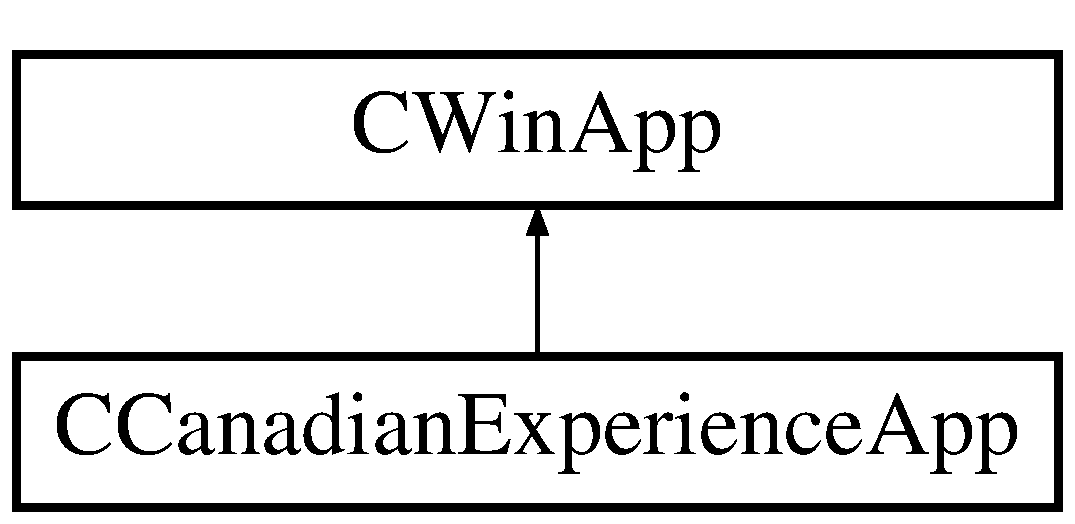
\includegraphics[height=2.000000cm]{class_c_canadian_experience_app}
\end{center}
\end{figure}
\subsection*{Public Member Functions}
\begin{DoxyCompactItemize}
\item 
virtual B\+O\+O\+L \hyperlink{class_c_canadian_experience_app_ab821deed5758f650a2fbbc65cefc8cc7}{Init\+Instance} ()
\begin{DoxyCompactList}\small\item\em \hyperlink{class_c_canadian_experience_app}{C\+Canadian\+Experience\+App} initialization. \end{DoxyCompactList}\item 
virtual int \hyperlink{class_c_canadian_experience_app_a289a9574888e0c922c455e73edf424ad}{Exit\+Instance} ()
\begin{DoxyCompactList}\small\item\em Exit this program. \end{DoxyCompactList}\item 
\hypertarget{class_c_canadian_experience_app_a99cb24a35f65d5821f7e09eefb0c97e7}{afx\+\_\+msg void \hyperlink{class_c_canadian_experience_app_a99cb24a35f65d5821f7e09eefb0c97e7}{On\+App\+About} ()}\label{class_c_canadian_experience_app_a99cb24a35f65d5821f7e09eefb0c97e7}

\begin{DoxyCompactList}\small\item\em App command to run the dialog. \end{DoxyCompactList}\end{DoxyCompactItemize}


\subsection{Detailed Description}
Program application class. 

\subsection{Member Function Documentation}
\hypertarget{class_c_canadian_experience_app_a289a9574888e0c922c455e73edf424ad}{\index{C\+Canadian\+Experience\+App@{C\+Canadian\+Experience\+App}!Exit\+Instance@{Exit\+Instance}}
\index{Exit\+Instance@{Exit\+Instance}!C\+Canadian\+Experience\+App@{C\+Canadian\+Experience\+App}}
\subsubsection[{Exit\+Instance}]{\setlength{\rightskip}{0pt plus 5cm}int C\+Canadian\+Experience\+App\+::\+Exit\+Instance (
\begin{DoxyParamCaption}
{}
\end{DoxyParamCaption}
)\hspace{0.3cm}{\ttfamily [virtual]}}}\label{class_c_canadian_experience_app_a289a9574888e0c922c455e73edf424ad}


Exit this program. 

\begin{DoxyReturn}{Returns}
exit code 
\end{DoxyReturn}
\hypertarget{class_c_canadian_experience_app_ab821deed5758f650a2fbbc65cefc8cc7}{\index{C\+Canadian\+Experience\+App@{C\+Canadian\+Experience\+App}!Init\+Instance@{Init\+Instance}}
\index{Init\+Instance@{Init\+Instance}!C\+Canadian\+Experience\+App@{C\+Canadian\+Experience\+App}}
\subsubsection[{Init\+Instance}]{\setlength{\rightskip}{0pt plus 5cm}B\+O\+O\+L C\+Canadian\+Experience\+App\+::\+Init\+Instance (
\begin{DoxyParamCaption}
{}
\end{DoxyParamCaption}
)\hspace{0.3cm}{\ttfamily [virtual]}}}\label{class_c_canadian_experience_app_ab821deed5758f650a2fbbc65cefc8cc7}


\hyperlink{class_c_canadian_experience_app}{C\+Canadian\+Experience\+App} initialization. 

\begin{DoxyReturn}{Returns}
T\+R\+U\+E if successful 
\end{DoxyReturn}


The documentation for this class was generated from the following files\+:\begin{DoxyCompactItemize}
\item 
\hyperlink{_canadian_experience_8h}{Canadian\+Experience.\+h}\item 
\hyperlink{_canadian_experience_8cpp}{Canadian\+Experience.\+cpp}\end{DoxyCompactItemize}

\hypertarget{class_c_drawable}{\section{C\+Drawable Class Reference}
\label{class_c_drawable}\index{C\+Drawable@{C\+Drawable}}
}


Abstract base class for drawable elements of our picture.  




{\ttfamily \#include $<$Drawable.\+h$>$}

Inheritance diagram for C\+Drawable\+:\begin{figure}[H]
\begin{center}
\leavevmode
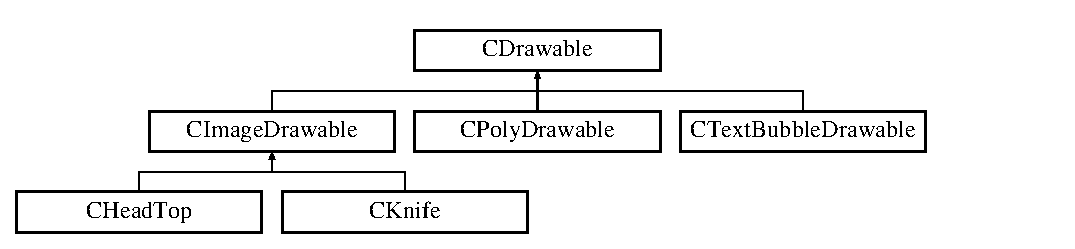
\includegraphics[height=2.896552cm]{class_c_drawable}
\end{center}
\end{figure}
\subsection*{Classes}
\begin{DoxyCompactItemize}
\item 
class \hyperlink{class_c_drawable_1_1_child_iter}{Child\+Iter}
\begin{DoxyCompactList}\small\item\em Iterator that iterates over the children of this drawable. \end{DoxyCompactList}\end{DoxyCompactItemize}
\subsection*{Public Member Functions}
\begin{DoxyCompactItemize}
\item 
\hypertarget{class_c_drawable_a58fd1036856d627b19976088e4143630}{virtual \hyperlink{class_c_drawable_a58fd1036856d627b19976088e4143630}{$\sim$\+C\+Drawable} ()}\label{class_c_drawable_a58fd1036856d627b19976088e4143630}

\begin{DoxyCompactList}\small\item\em Destructor. \end{DoxyCompactList}\item 
\hypertarget{class_c_drawable_abd46d61baf3d5f5210aa3c66b98d9263}{\hyperlink{class_c_drawable_abd46d61baf3d5f5210aa3c66b98d9263}{C\+Drawable} ()=delete}\label{class_c_drawable_abd46d61baf3d5f5210aa3c66b98d9263}

\begin{DoxyCompactList}\small\item\em Default constructor disabled. \end{DoxyCompactList}\item 
\hypertarget{class_c_drawable_abec99c088c1a7c12e1d7ecae69135602}{\hyperlink{class_c_drawable_abec99c088c1a7c12e1d7ecae69135602}{C\+Drawable} (const \hyperlink{class_c_drawable}{C\+Drawable} \&)=delete}\label{class_c_drawable_abec99c088c1a7c12e1d7ecae69135602}

\begin{DoxyCompactList}\small\item\em Copy constructor disabled. \end{DoxyCompactList}\item 
\hypertarget{class_c_drawable_aabd5f52b903e57a4c8b145cb69158adb}{void \hyperlink{class_c_drawable_aabd5f52b903e57a4c8b145cb69158adb}{operator=} (const \hyperlink{class_c_drawable}{C\+Drawable} \&)=delete}\label{class_c_drawable_aabd5f52b903e57a4c8b145cb69158adb}

\begin{DoxyCompactList}\small\item\em Assignment operator disabled. \end{DoxyCompactList}\item 
virtual void \hyperlink{class_c_drawable_a86762c6e220d9f502c6ccf9baf1135ac}{Set\+Actor} (\hyperlink{class_c_actor}{C\+Actor} $\ast$actor)
\begin{DoxyCompactList}\small\item\em Set the actor using this drawable. \end{DoxyCompactList}\item 
virtual void \hyperlink{class_c_drawable_a9b6a9920a75d88d9ae321997495eaec7}{Draw} (Gdiplus\+::\+Graphics $\ast$graphics)=0
\begin{DoxyCompactList}\small\item\em Draw the drawable. \end{DoxyCompactList}\item 
void \hyperlink{class_c_drawable_ac154be14313b739471d3a1529a2b31b5}{Place} (Gdiplus\+::\+Point offset, double rotate)
\begin{DoxyCompactList}\small\item\em Place this drawable relative to its parent. \end{DoxyCompactList}\item 
void \hyperlink{class_c_drawable_ab636167462699dde9b80e6dcb08caf7c}{Add\+Child} (std\+::shared\+\_\+ptr$<$ \hyperlink{class_c_drawable}{C\+Drawable} $>$ child)
\begin{DoxyCompactList}\small\item\em Add a child drawable to this drawable. \end{DoxyCompactList}\item 
virtual bool \hyperlink{class_c_drawable_a43490aec87b1209bbf7441e3855f0874}{Hit\+Test} (Gdiplus\+::\+Point pos)=0
\begin{DoxyCompactList}\small\item\em Test to see if we have been clicked on by the mouse. \end{DoxyCompactList}\item 
virtual bool \hyperlink{class_c_drawable_ac9f03cfc58aed75fb52cd69c71e7b6e0}{Is\+Movable} ()
\begin{DoxyCompactList}\small\item\em Is this a movable drawable? \end{DoxyCompactList}\item 
void \hyperlink{class_c_drawable_a2241b02a5f50c7a455283a9fb24d5b27}{Move} (Gdiplus\+::\+Point delta)
\begin{DoxyCompactList}\small\item\em Move this drawable some amount. \end{DoxyCompactList}\item 
void \hyperlink{class_c_drawable_aa6b8988df847a76c30dfcf525ab65449}{Set\+Position} (Gdiplus\+::\+Point pos)
\begin{DoxyCompactList}\small\item\em Set the drawable position. \end{DoxyCompactList}\item 
Gdiplus\+::\+Point \hyperlink{class_c_drawable_ac1def1d34d8069e3985e3a423ba80f2d}{Get\+Position} () const 
\begin{DoxyCompactList}\small\item\em Get the drawable position. \end{DoxyCompactList}\item 
void \hyperlink{class_c_drawable_ab1191ba99b869690839ff20cd0cc45c4}{Set\+Rotation} (double r)
\begin{DoxyCompactList}\small\item\em Set the rotation angle in radians. \end{DoxyCompactList}\item 
double \hyperlink{class_c_drawable_afb31912cfe47cc336dfbef384181ca65}{Get\+Rotation} () const 
\begin{DoxyCompactList}\small\item\em Get the rotation angle in radians. \end{DoxyCompactList}\item 
std\+::wstring \hyperlink{class_c_drawable_a45af045c285cd0be9340a9a0d9883260}{Get\+Name} () const 
\begin{DoxyCompactList}\small\item\em Get the drawable name. \end{DoxyCompactList}\item 
void \hyperlink{class_c_drawable_ad53fc2430248f2ac022ab142024df983}{Set\+Parent} (\hyperlink{class_c_drawable}{C\+Drawable} $\ast$parent)
\begin{DoxyCompactList}\small\item\em Set the drawable parent. \end{DoxyCompactList}\item 
\hyperlink{class_c_drawable}{C\+Drawable} $\ast$ \hyperlink{class_c_drawable_a7f71959d8c597e34abb395b6dece5ad6}{Get\+Parent} ()
\begin{DoxyCompactList}\small\item\em Get the drawable parent. \end{DoxyCompactList}\item 
virtual bool \hyperlink{class_c_drawable_a43bc0016ffe1bfe22f5b97730c431514}{Is\+Text\+Bubble\+Drawable} ()
\begin{DoxyCompactList}\small\item\em Check the drawable is Text\+Bubble\+Drawable. \end{DoxyCompactList}\item 
\hyperlink{class_c_drawable_1_1_child_iter}{Child\+Iter} \hyperlink{class_c_drawable_a8a369d10744f4139f8d39da8806fb4be}{begin} ()
\begin{DoxyCompactList}\small\item\em Get an iterator for the beginning of the collection. \end{DoxyCompactList}\item 
\hyperlink{class_c_drawable_1_1_child_iter}{Child\+Iter} \hyperlink{class_c_drawable_a44ad4b912b744487eb0bac2328e86336}{end} ()
\begin{DoxyCompactList}\small\item\em Get an iterator for the end of the collection. \end{DoxyCompactList}\item 
virtual void \hyperlink{class_c_drawable_a479df46ae298bf716d96b05b1ba6e529}{Set\+Timeline} (\hyperlink{class_c_timeline}{C\+Timeline} $\ast$timeline)
\item 
\hypertarget{class_c_drawable_acd0be14f2f8666ce8f57db68dd220308}{virtual void \hyperlink{class_c_drawable_acd0be14f2f8666ce8f57db68dd220308}{Set\+Keyframe} ()}\label{class_c_drawable_acd0be14f2f8666ce8f57db68dd220308}

\begin{DoxyCompactList}\small\item\em Set the keyframe based on the current status. \end{DoxyCompactList}\item 
\hypertarget{class_c_drawable_aad6d3c8e4c1ad3715c8aa56e2a83977d}{virtual void \hyperlink{class_c_drawable_aad6d3c8e4c1ad3715c8aa56e2a83977d}{Get\+Keyframe} ()}\label{class_c_drawable_aad6d3c8e4c1ad3715c8aa56e2a83977d}

\begin{DoxyCompactList}\small\item\em Get the current channel from the animation system. \end{DoxyCompactList}\item 
\hyperlink{class_c_anim_channel_angle}{C\+Anim\+Channel\+Angle} $\ast$ \hyperlink{class_c_drawable_a14665f0fbbfa93bb349f7993a7af5de4}{Get\+Angle\+Channel} ()
\begin{DoxyCompactList}\small\item\em The angle animation channel. \end{DoxyCompactList}\item 
virtual C\+Text\+Bubble $\ast$ \hyperlink{class_c_drawable_ac271ee6f71e550946b5da8f27d0ff6be}{Get\+Text\+Bubble} ()
\begin{DoxyCompactList}\small\item\em The text animation channel. \end{DoxyCompactList}\end{DoxyCompactItemize}
\subsection*{Protected Member Functions}
\begin{DoxyCompactItemize}
\item 
\hyperlink{class_c_drawable_a2e153d7fd3a752139b0b87ea990a25fc}{C\+Drawable} (const std\+::wstring \&name)
\begin{DoxyCompactList}\small\item\em Constructor. \end{DoxyCompactList}\item 
Gdiplus\+::\+Point \hyperlink{class_c_drawable_aabf32ebc32a2dbe928bc9fa38bd82535}{Rotate\+Point} (Gdiplus\+::\+Point point, double angle)
\begin{DoxyCompactList}\small\item\em Rotate a point by a given angle. \end{DoxyCompactList}\end{DoxyCompactItemize}
\subsection*{Protected Attributes}
\begin{DoxyCompactItemize}
\item 
\hypertarget{class_c_drawable_abafce2c99898aac71bdb99ec2031d3a5}{Gdiplus\+::\+Point \hyperlink{class_c_drawable_abafce2c99898aac71bdb99ec2031d3a5}{m\+Placed\+Position} = Gdiplus\+::\+Point(0, 0)}\label{class_c_drawable_abafce2c99898aac71bdb99ec2031d3a5}

\begin{DoxyCompactList}\small\item\em The actual postion in the drawing. \end{DoxyCompactList}\item 
\hypertarget{class_c_drawable_a3b280b16b1a4a8c6e2588b1dc5574bda}{double \hyperlink{class_c_drawable_a3b280b16b1a4a8c6e2588b1dc5574bda}{m\+Placed\+R} = 0}\label{class_c_drawable_a3b280b16b1a4a8c6e2588b1dc5574bda}

\begin{DoxyCompactList}\small\item\em The actual rotation in the drawing. \end{DoxyCompactList}\end{DoxyCompactItemize}


\subsection{Detailed Description}
Abstract base class for drawable elements of our picture. 

A drawable is one part of an actor. Drawable parts can be moved independently. 

\subsection{Constructor \& Destructor Documentation}
\hypertarget{class_c_drawable_a2e153d7fd3a752139b0b87ea990a25fc}{\index{C\+Drawable@{C\+Drawable}!C\+Drawable@{C\+Drawable}}
\index{C\+Drawable@{C\+Drawable}!C\+Drawable@{C\+Drawable}}
\subsubsection[{C\+Drawable}]{\setlength{\rightskip}{0pt plus 5cm}C\+Drawable\+::\+C\+Drawable (
\begin{DoxyParamCaption}
\item[{const std\+::wstring \&}]{name}
\end{DoxyParamCaption}
)\hspace{0.3cm}{\ttfamily [protected]}}}\label{class_c_drawable_a2e153d7fd3a752139b0b87ea990a25fc}


Constructor. 


\begin{DoxyParams}{Parameters}
{\em name} & The drawable name \\
\hline
\end{DoxyParams}


\subsection{Member Function Documentation}
\hypertarget{class_c_drawable_ab636167462699dde9b80e6dcb08caf7c}{\index{C\+Drawable@{C\+Drawable}!Add\+Child@{Add\+Child}}
\index{Add\+Child@{Add\+Child}!C\+Drawable@{C\+Drawable}}
\subsubsection[{Add\+Child}]{\setlength{\rightskip}{0pt plus 5cm}void C\+Drawable\+::\+Add\+Child (
\begin{DoxyParamCaption}
\item[{std\+::shared\+\_\+ptr$<$ {\bf C\+Drawable} $>$}]{child}
\end{DoxyParamCaption}
)}}\label{class_c_drawable_ab636167462699dde9b80e6dcb08caf7c}


Add a child drawable to this drawable. 


\begin{DoxyParams}{Parameters}
{\em child} & The child to add \\
\hline
\end{DoxyParams}
\hypertarget{class_c_drawable_a8a369d10744f4139f8d39da8806fb4be}{\index{C\+Drawable@{C\+Drawable}!begin@{begin}}
\index{begin@{begin}!C\+Drawable@{C\+Drawable}}
\subsubsection[{begin}]{\setlength{\rightskip}{0pt plus 5cm}{\bf Child\+Iter} C\+Drawable\+::begin (
\begin{DoxyParamCaption}
{}
\end{DoxyParamCaption}
)\hspace{0.3cm}{\ttfamily [inline]}}}\label{class_c_drawable_a8a369d10744f4139f8d39da8806fb4be}


Get an iterator for the beginning of the collection. 

\begin{DoxyReturn}{Returns}
Iter object at position 0 
\end{DoxyReturn}
\hypertarget{class_c_drawable_a9b6a9920a75d88d9ae321997495eaec7}{\index{C\+Drawable@{C\+Drawable}!Draw@{Draw}}
\index{Draw@{Draw}!C\+Drawable@{C\+Drawable}}
\subsubsection[{Draw}]{\setlength{\rightskip}{0pt plus 5cm}virtual void C\+Drawable\+::\+Draw (
\begin{DoxyParamCaption}
\item[{Gdiplus\+::\+Graphics $\ast$}]{graphics}
\end{DoxyParamCaption}
)\hspace{0.3cm}{\ttfamily [pure virtual]}}}\label{class_c_drawable_a9b6a9920a75d88d9ae321997495eaec7}


Draw the drawable. 


\begin{DoxyParams}{Parameters}
{\em graphics} & Graphics object to draw on \\
\hline
\end{DoxyParams}


Implemented in \hyperlink{class_c_head_top_aa77d9fa703079ee68a4e4e8e3c816932}{C\+Head\+Top}, \hyperlink{class_c_text_bubble_drawable_ab06c08f5357aabd1275610baac806b59}{C\+Text\+Bubble\+Drawable}, \hyperlink{class_c_poly_drawable_a701f45c8fabdec3de96b3048aa3a0190}{C\+Poly\+Drawable}, \hyperlink{class_c_knife_a71b0ee76740242e1e04f1f1500422ca3}{C\+Knife}, and \hyperlink{class_c_image_drawable_ada4d5d342230fbecb7169e4f3324ee52}{C\+Image\+Drawable}.

\hypertarget{class_c_drawable_a44ad4b912b744487eb0bac2328e86336}{\index{C\+Drawable@{C\+Drawable}!end@{end}}
\index{end@{end}!C\+Drawable@{C\+Drawable}}
\subsubsection[{end}]{\setlength{\rightskip}{0pt plus 5cm}{\bf Child\+Iter} C\+Drawable\+::end (
\begin{DoxyParamCaption}
{}
\end{DoxyParamCaption}
)\hspace{0.3cm}{\ttfamily [inline]}}}\label{class_c_drawable_a44ad4b912b744487eb0bac2328e86336}


Get an iterator for the end of the collection. 

\begin{DoxyReturn}{Returns}
Iter object at position past the end 
\end{DoxyReturn}
\hypertarget{class_c_drawable_a14665f0fbbfa93bb349f7993a7af5de4}{\index{C\+Drawable@{C\+Drawable}!Get\+Angle\+Channel@{Get\+Angle\+Channel}}
\index{Get\+Angle\+Channel@{Get\+Angle\+Channel}!C\+Drawable@{C\+Drawable}}
\subsubsection[{Get\+Angle\+Channel}]{\setlength{\rightskip}{0pt plus 5cm}{\bf C\+Anim\+Channel\+Angle}$\ast$ C\+Drawable\+::\+Get\+Angle\+Channel (
\begin{DoxyParamCaption}
{}
\end{DoxyParamCaption}
)\hspace{0.3cm}{\ttfamily [inline]}}}\label{class_c_drawable_a14665f0fbbfa93bb349f7993a7af5de4}


The angle animation channel. 

\begin{DoxyReturn}{Returns}
Pointer to animation channel 
\end{DoxyReturn}
\hypertarget{class_c_drawable_a45af045c285cd0be9340a9a0d9883260}{\index{C\+Drawable@{C\+Drawable}!Get\+Name@{Get\+Name}}
\index{Get\+Name@{Get\+Name}!C\+Drawable@{C\+Drawable}}
\subsubsection[{Get\+Name}]{\setlength{\rightskip}{0pt plus 5cm}std\+::wstring C\+Drawable\+::\+Get\+Name (
\begin{DoxyParamCaption}
{}
\end{DoxyParamCaption}
) const\hspace{0.3cm}{\ttfamily [inline]}}}\label{class_c_drawable_a45af045c285cd0be9340a9a0d9883260}


Get the drawable name. 

\begin{DoxyReturn}{Returns}
The drawable name 
\end{DoxyReturn}
\hypertarget{class_c_drawable_a7f71959d8c597e34abb395b6dece5ad6}{\index{C\+Drawable@{C\+Drawable}!Get\+Parent@{Get\+Parent}}
\index{Get\+Parent@{Get\+Parent}!C\+Drawable@{C\+Drawable}}
\subsubsection[{Get\+Parent}]{\setlength{\rightskip}{0pt plus 5cm}{\bf C\+Drawable}$\ast$ C\+Drawable\+::\+Get\+Parent (
\begin{DoxyParamCaption}
{}
\end{DoxyParamCaption}
)\hspace{0.3cm}{\ttfamily [inline]}}}\label{class_c_drawable_a7f71959d8c597e34abb395b6dece5ad6}


Get the drawable parent. 

\begin{DoxyReturn}{Returns}
Parent pointer 
\end{DoxyReturn}
\hypertarget{class_c_drawable_ac1def1d34d8069e3985e3a423ba80f2d}{\index{C\+Drawable@{C\+Drawable}!Get\+Position@{Get\+Position}}
\index{Get\+Position@{Get\+Position}!C\+Drawable@{C\+Drawable}}
\subsubsection[{Get\+Position}]{\setlength{\rightskip}{0pt plus 5cm}Gdiplus\+::\+Point C\+Drawable\+::\+Get\+Position (
\begin{DoxyParamCaption}
{}
\end{DoxyParamCaption}
) const\hspace{0.3cm}{\ttfamily [inline]}}}\label{class_c_drawable_ac1def1d34d8069e3985e3a423ba80f2d}


Get the drawable position. 

\begin{DoxyReturn}{Returns}
The drawable position 
\end{DoxyReturn}
\hypertarget{class_c_drawable_afb31912cfe47cc336dfbef384181ca65}{\index{C\+Drawable@{C\+Drawable}!Get\+Rotation@{Get\+Rotation}}
\index{Get\+Rotation@{Get\+Rotation}!C\+Drawable@{C\+Drawable}}
\subsubsection[{Get\+Rotation}]{\setlength{\rightskip}{0pt plus 5cm}double C\+Drawable\+::\+Get\+Rotation (
\begin{DoxyParamCaption}
{}
\end{DoxyParamCaption}
) const\hspace{0.3cm}{\ttfamily [inline]}}}\label{class_c_drawable_afb31912cfe47cc336dfbef384181ca65}


Get the rotation angle in radians. 

\begin{DoxyReturn}{Returns}
The rotation angle in radians 
\end{DoxyReturn}
\hypertarget{class_c_drawable_ac271ee6f71e550946b5da8f27d0ff6be}{\index{C\+Drawable@{C\+Drawable}!Get\+Text\+Bubble@{Get\+Text\+Bubble}}
\index{Get\+Text\+Bubble@{Get\+Text\+Bubble}!C\+Drawable@{C\+Drawable}}
\subsubsection[{Get\+Text\+Bubble}]{\setlength{\rightskip}{0pt plus 5cm}virtual C\+Text\+Bubble$\ast$ C\+Drawable\+::\+Get\+Text\+Bubble (
\begin{DoxyParamCaption}
{}
\end{DoxyParamCaption}
)\hspace{0.3cm}{\ttfamily [inline]}, {\ttfamily [virtual]}}}\label{class_c_drawable_ac271ee6f71e550946b5da8f27d0ff6be}


The text animation channel. 

\begin{DoxyReturn}{Returns}
Pointer to animation channel 
\end{DoxyReturn}


Reimplemented in \hyperlink{class_c_text_bubble_drawable_a0df72f52a5df614eccdff89bf12cf905}{C\+Text\+Bubble\+Drawable}.

\hypertarget{class_c_drawable_a43490aec87b1209bbf7441e3855f0874}{\index{C\+Drawable@{C\+Drawable}!Hit\+Test@{Hit\+Test}}
\index{Hit\+Test@{Hit\+Test}!C\+Drawable@{C\+Drawable}}
\subsubsection[{Hit\+Test}]{\setlength{\rightskip}{0pt plus 5cm}bool C\+Drawable\+::\+Hit\+Test (
\begin{DoxyParamCaption}
\item[{Gdiplus\+::\+Point}]{pos}
\end{DoxyParamCaption}
)\hspace{0.3cm}{\ttfamily [pure virtual]}}}\label{class_c_drawable_a43490aec87b1209bbf7441e3855f0874}


Test to see if we have been clicked on by the mouse. 

Test to see if we clicked on this drawable.


\begin{DoxyParams}{Parameters}
{\em pos} & Position to test \\
\hline
\end{DoxyParams}
\begin{DoxyReturn}{Returns}
true if clicked on
\end{DoxyReturn}

\begin{DoxyParams}{Parameters}
{\em pos} & Position we clicked \\
\hline
\end{DoxyParams}
\begin{DoxyReturn}{Returns}
True if we clicked on it 
\end{DoxyReturn}


Implemented in \hyperlink{class_c_text_bubble_drawable_a85dd41fa9b6ce12989f529907030fd9a}{C\+Text\+Bubble\+Drawable}, \hyperlink{class_c_poly_drawable_a4db3493e3bba3c4c51608a75d48f50e2}{C\+Poly\+Drawable}, and \hyperlink{class_c_image_drawable_a8aac5e64e309f1990e757f564dbcb8fd}{C\+Image\+Drawable}.

\hypertarget{class_c_drawable_ac9f03cfc58aed75fb52cd69c71e7b6e0}{\index{C\+Drawable@{C\+Drawable}!Is\+Movable@{Is\+Movable}}
\index{Is\+Movable@{Is\+Movable}!C\+Drawable@{C\+Drawable}}
\subsubsection[{Is\+Movable}]{\setlength{\rightskip}{0pt plus 5cm}virtual bool C\+Drawable\+::\+Is\+Movable (
\begin{DoxyParamCaption}
{}
\end{DoxyParamCaption}
)\hspace{0.3cm}{\ttfamily [inline]}, {\ttfamily [virtual]}}}\label{class_c_drawable_ac9f03cfc58aed75fb52cd69c71e7b6e0}


Is this a movable drawable? 

\begin{DoxyReturn}{Returns}
true if movable 
\end{DoxyReturn}


Reimplemented in \hyperlink{class_c_text_bubble_drawable_aa12d719c3c6e7d76edc3d0afdb5e9485}{C\+Text\+Bubble\+Drawable}, \hyperlink{class_c_head_top_a853b7d9f248dc36519f1da6c4d53b18e}{C\+Head\+Top}, and \hyperlink{class_c_knife_a838e9409d22b1cc04d584abc611b65e6}{C\+Knife}.

\hypertarget{class_c_drawable_a43bc0016ffe1bfe22f5b97730c431514}{\index{C\+Drawable@{C\+Drawable}!Is\+Text\+Bubble\+Drawable@{Is\+Text\+Bubble\+Drawable}}
\index{Is\+Text\+Bubble\+Drawable@{Is\+Text\+Bubble\+Drawable}!C\+Drawable@{C\+Drawable}}
\subsubsection[{Is\+Text\+Bubble\+Drawable}]{\setlength{\rightskip}{0pt plus 5cm}virtual bool C\+Drawable\+::\+Is\+Text\+Bubble\+Drawable (
\begin{DoxyParamCaption}
{}
\end{DoxyParamCaption}
)\hspace{0.3cm}{\ttfamily [inline]}, {\ttfamily [virtual]}}}\label{class_c_drawable_a43bc0016ffe1bfe22f5b97730c431514}


Check the drawable is Text\+Bubble\+Drawable. 

\begin{DoxyReturn}{Returns}
a bool value 
\end{DoxyReturn}


Reimplemented in \hyperlink{class_c_text_bubble_drawable_a0ad09643af72c6fcd0182f38e8ce18da}{C\+Text\+Bubble\+Drawable}.

\hypertarget{class_c_drawable_a2241b02a5f50c7a455283a9fb24d5b27}{\index{C\+Drawable@{C\+Drawable}!Move@{Move}}
\index{Move@{Move}!C\+Drawable@{C\+Drawable}}
\subsubsection[{Move}]{\setlength{\rightskip}{0pt plus 5cm}void C\+Drawable\+::\+Move (
\begin{DoxyParamCaption}
\item[{Gdiplus\+::\+Point}]{delta}
\end{DoxyParamCaption}
)}}\label{class_c_drawable_a2241b02a5f50c7a455283a9fb24d5b27}


Move this drawable some amount. 


\begin{DoxyParams}{Parameters}
{\em delta} & The amount to move \\
\hline
\end{DoxyParams}
\hypertarget{class_c_drawable_ac154be14313b739471d3a1529a2b31b5}{\index{C\+Drawable@{C\+Drawable}!Place@{Place}}
\index{Place@{Place}!C\+Drawable@{C\+Drawable}}
\subsubsection[{Place}]{\setlength{\rightskip}{0pt plus 5cm}void C\+Drawable\+::\+Place (
\begin{DoxyParamCaption}
\item[{Gdiplus\+::\+Point}]{offset, }
\item[{double}]{rotate}
\end{DoxyParamCaption}
)}}\label{class_c_drawable_ac154be14313b739471d3a1529a2b31b5}


Place this drawable relative to its parent. 

This works hierarchically from top item down. 
\begin{DoxyParams}{Parameters}
{\em offset} & Parent offset \\
\hline
{\em rotate} & Parent rotation \\
\hline
\end{DoxyParams}
\hypertarget{class_c_drawable_aabf32ebc32a2dbe928bc9fa38bd82535}{\index{C\+Drawable@{C\+Drawable}!Rotate\+Point@{Rotate\+Point}}
\index{Rotate\+Point@{Rotate\+Point}!C\+Drawable@{C\+Drawable}}
\subsubsection[{Rotate\+Point}]{\setlength{\rightskip}{0pt plus 5cm}Gdiplus\+::\+Point C\+Drawable\+::\+Rotate\+Point (
\begin{DoxyParamCaption}
\item[{Gdiplus\+::\+Point}]{point, }
\item[{double}]{angle}
\end{DoxyParamCaption}
)\hspace{0.3cm}{\ttfamily [protected]}}}\label{class_c_drawable_aabf32ebc32a2dbe928bc9fa38bd82535}


Rotate a point by a given angle. 


\begin{DoxyParams}{Parameters}
{\em point} & The point to rotate \\
\hline
{\em angle} & An angle in radians \\
\hline
\end{DoxyParams}
\begin{DoxyReturn}{Returns}
Rotated point 
\end{DoxyReturn}
\hypertarget{class_c_drawable_a86762c6e220d9f502c6ccf9baf1135ac}{\index{C\+Drawable@{C\+Drawable}!Set\+Actor@{Set\+Actor}}
\index{Set\+Actor@{Set\+Actor}!C\+Drawable@{C\+Drawable}}
\subsubsection[{Set\+Actor}]{\setlength{\rightskip}{0pt plus 5cm}void C\+Drawable\+::\+Set\+Actor (
\begin{DoxyParamCaption}
\item[{{\bf C\+Actor} $\ast$}]{actor}
\end{DoxyParamCaption}
)\hspace{0.3cm}{\ttfamily [virtual]}}}\label{class_c_drawable_a86762c6e220d9f502c6ccf9baf1135ac}


Set the actor using this drawable. 


\begin{DoxyParams}{Parameters}
{\em actor} & Actor using this drawable \\
\hline
\end{DoxyParams}


Reimplemented in \hyperlink{class_c_head_top_a740ff72a9e96c8407a858079f14f0ad3}{C\+Head\+Top}, \hyperlink{class_c_text_bubble_drawable_a6e154d1a283f3f0b85eb1f3d1480c21e}{C\+Text\+Bubble\+Drawable}, and \hyperlink{class_c_knife_a1586c8502c39cd3032785d946a1f3f73}{C\+Knife}.

\hypertarget{class_c_drawable_ad53fc2430248f2ac022ab142024df983}{\index{C\+Drawable@{C\+Drawable}!Set\+Parent@{Set\+Parent}}
\index{Set\+Parent@{Set\+Parent}!C\+Drawable@{C\+Drawable}}
\subsubsection[{Set\+Parent}]{\setlength{\rightskip}{0pt plus 5cm}void C\+Drawable\+::\+Set\+Parent (
\begin{DoxyParamCaption}
\item[{{\bf C\+Drawable} $\ast$}]{parent}
\end{DoxyParamCaption}
)\hspace{0.3cm}{\ttfamily [inline]}}}\label{class_c_drawable_ad53fc2430248f2ac022ab142024df983}


Set the drawable parent. 


\begin{DoxyParams}{Parameters}
{\em parent} & New parent pointer \\
\hline
\end{DoxyParams}
\hypertarget{class_c_drawable_aa6b8988df847a76c30dfcf525ab65449}{\index{C\+Drawable@{C\+Drawable}!Set\+Position@{Set\+Position}}
\index{Set\+Position@{Set\+Position}!C\+Drawable@{C\+Drawable}}
\subsubsection[{Set\+Position}]{\setlength{\rightskip}{0pt plus 5cm}void C\+Drawable\+::\+Set\+Position (
\begin{DoxyParamCaption}
\item[{Gdiplus\+::\+Point}]{pos}
\end{DoxyParamCaption}
)\hspace{0.3cm}{\ttfamily [inline]}}}\label{class_c_drawable_aa6b8988df847a76c30dfcf525ab65449}


Set the drawable position. 


\begin{DoxyParams}{Parameters}
{\em pos} & The new drawable position \\
\hline
\end{DoxyParams}
\hypertarget{class_c_drawable_ab1191ba99b869690839ff20cd0cc45c4}{\index{C\+Drawable@{C\+Drawable}!Set\+Rotation@{Set\+Rotation}}
\index{Set\+Rotation@{Set\+Rotation}!C\+Drawable@{C\+Drawable}}
\subsubsection[{Set\+Rotation}]{\setlength{\rightskip}{0pt plus 5cm}void C\+Drawable\+::\+Set\+Rotation (
\begin{DoxyParamCaption}
\item[{double}]{r}
\end{DoxyParamCaption}
)\hspace{0.3cm}{\ttfamily [inline]}}}\label{class_c_drawable_ab1191ba99b869690839ff20cd0cc45c4}


Set the rotation angle in radians. 


\begin{DoxyParams}{Parameters}
{\em r} & The new rotation angle in radians \\
\hline
\end{DoxyParams}
\hypertarget{class_c_drawable_a479df46ae298bf716d96b05b1ba6e529}{\index{C\+Drawable@{C\+Drawable}!Set\+Timeline@{Set\+Timeline}}
\index{Set\+Timeline@{Set\+Timeline}!C\+Drawable@{C\+Drawable}}
\subsubsection[{Set\+Timeline}]{\setlength{\rightskip}{0pt plus 5cm}void C\+Drawable\+::\+Set\+Timeline (
\begin{DoxyParamCaption}
\item[{{\bf C\+Timeline} $\ast$}]{timeline}
\end{DoxyParamCaption}
)\hspace{0.3cm}{\ttfamily [virtual]}}}\label{class_c_drawable_a479df46ae298bf716d96b05b1ba6e529}
Add the channels for this drawable to a timeline 
\begin{DoxyParams}{Parameters}
{\em timeline} & The timeline class. \\
\hline
\end{DoxyParams}


Reimplemented in \hyperlink{class_c_head_top_a379aaabd0a8d4a80751341bccc2faeda}{C\+Head\+Top}, \hyperlink{class_c_text_bubble_drawable_adbf6b04696680906cc3cb32e7a0918b9}{C\+Text\+Bubble\+Drawable}, and \hyperlink{class_c_knife_a74c7de63a301d48c10b9dd0ad2c45735}{C\+Knife}.



The documentation for this class was generated from the following files\+:\begin{DoxyCompactItemize}
\item 
\hyperlink{_drawable_8h}{Drawable.\+h}\item 
\hyperlink{_drawable_8cpp}{Drawable.\+cpp}\end{DoxyCompactItemize}

\hypertarget{class_c_harold_factory}{\section{C\+Harold\+Factory Class Reference}
\label{class_c_harold_factory}\index{C\+Harold\+Factory@{C\+Harold\+Factory}}
}


Factory class that builds the Harold character.  




{\ttfamily \#include $<$Harold\+Factory.\+h$>$}

Inheritance diagram for C\+Harold\+Factory\+:\begin{figure}[H]
\begin{center}
\leavevmode
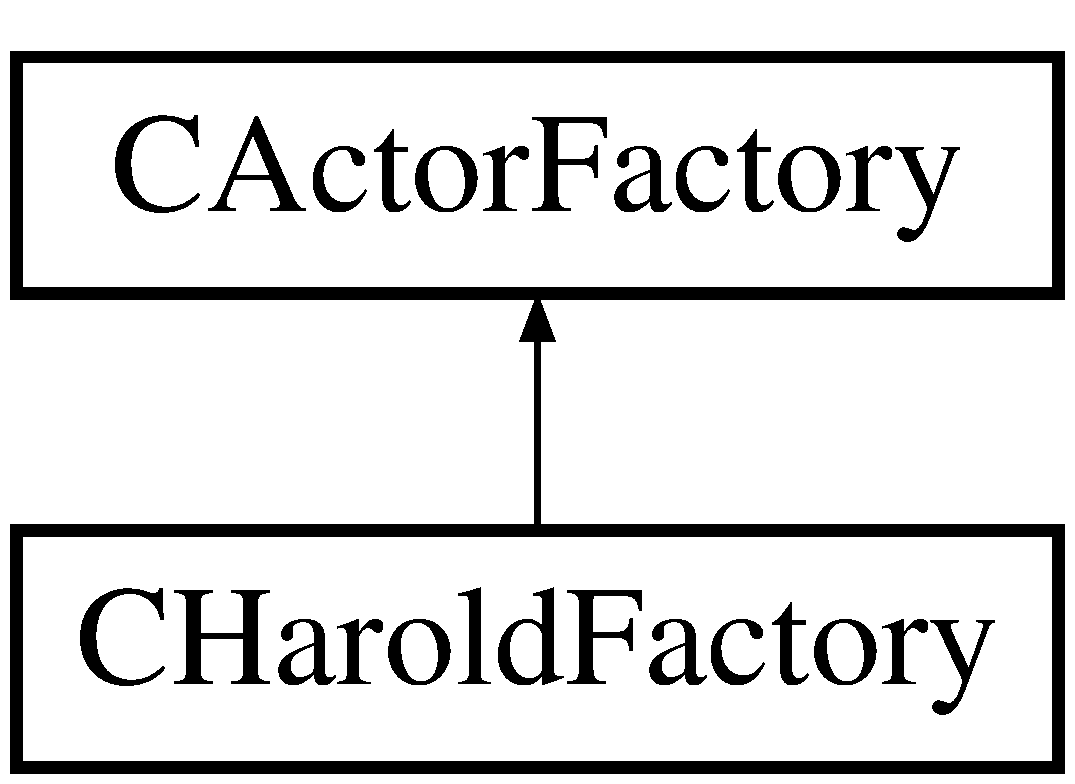
\includegraphics[height=2.000000cm]{class_c_harold_factory}
\end{center}
\end{figure}
\subsection*{Public Member Functions}
\begin{DoxyCompactItemize}
\item 
std\+::shared\+\_\+ptr$<$ \hyperlink{class_c_actor}{C\+Actor} $>$ \hyperlink{class_c_harold_factory_a785f8194f83d866bfc2a237fc3d4abc1}{Create} ()
\begin{DoxyCompactList}\small\item\em This is a concrete factory method that creates our Harold actor. \end{DoxyCompactList}\end{DoxyCompactItemize}
\subsection*{Additional Inherited Members}


\subsection{Detailed Description}
Factory class that builds the Harold character. 

\subsection{Member Function Documentation}
\hypertarget{class_c_harold_factory_a785f8194f83d866bfc2a237fc3d4abc1}{\index{C\+Harold\+Factory@{C\+Harold\+Factory}!Create@{Create}}
\index{Create@{Create}!C\+Harold\+Factory@{C\+Harold\+Factory}}
\subsubsection[{Create}]{\setlength{\rightskip}{0pt plus 5cm}std\+::shared\+\_\+ptr$<$ {\bf C\+Actor} $>$ C\+Harold\+Factory\+::\+Create (
\begin{DoxyParamCaption}
{}
\end{DoxyParamCaption}
)\hspace{0.3cm}{\ttfamily [virtual]}}}\label{class_c_harold_factory_a785f8194f83d866bfc2a237fc3d4abc1}


This is a concrete factory method that creates our Harold actor. 

\begin{DoxyReturn}{Returns}
Pointer to an actor object. 
\end{DoxyReturn}


Implements \hyperlink{class_c_actor_factory_a1e751d97cc015ab2182b7683133e5a5d}{C\+Actor\+Factory}.



The documentation for this class was generated from the following files\+:\begin{DoxyCompactItemize}
\item 
\hyperlink{_harold_factory_8h}{Harold\+Factory.\+h}\item 
\hyperlink{_harold_factory_8cpp}{Harold\+Factory.\+cpp}\end{DoxyCompactItemize}

\hypertarget{class_c_head_top}{\section{C\+Head\+Top Class Reference}
\label{class_c_head_top}\index{C\+Head\+Top@{C\+Head\+Top}}
}


Implements the top of a characters head, which has special functionality.  




{\ttfamily \#include $<$Head\+Top.\+h$>$}

Inheritance diagram for C\+Head\+Top\+:\begin{figure}[H]
\begin{center}
\leavevmode
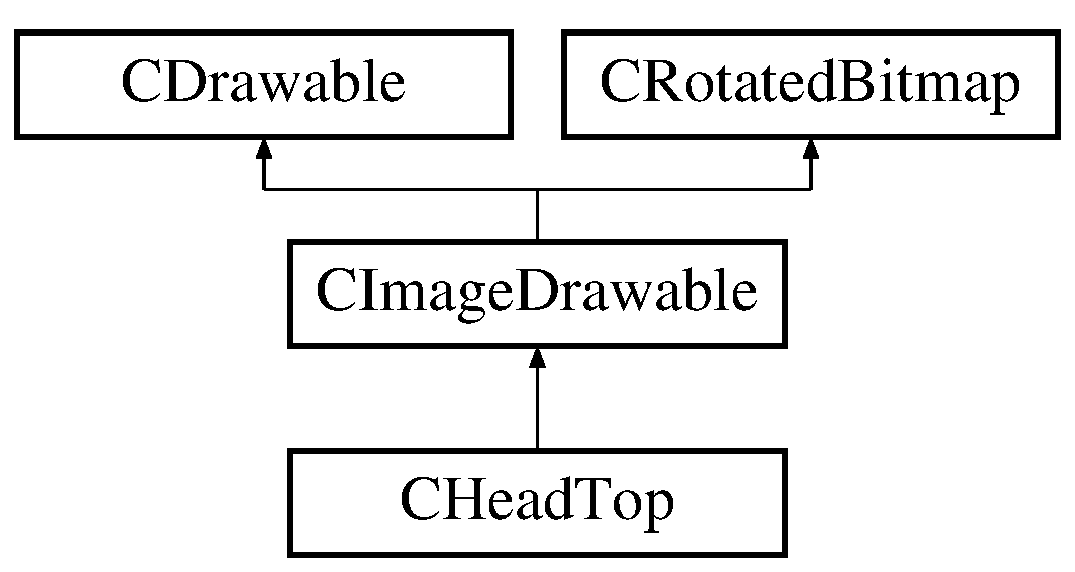
\includegraphics[height=3.000000cm]{class_c_head_top}
\end{center}
\end{figure}
\subsection*{Public Member Functions}
\begin{DoxyCompactItemize}
\item 
\hyperlink{class_c_head_top_a31333179dc1836d6ae5b9636b215b66b}{C\+Head\+Top} (const std\+::wstring \&name, const std\+::wstring \&filename)
\begin{DoxyCompactList}\small\item\em Constructor for a top of the head object. \end{DoxyCompactList}\item 
\hypertarget{class_c_head_top_a64697c81bc0100f66aa661a8bc430fa9}{\hyperlink{class_c_head_top_a64697c81bc0100f66aa661a8bc430fa9}{$\sim$\+C\+Head\+Top} ()}\label{class_c_head_top_a64697c81bc0100f66aa661a8bc430fa9}

\begin{DoxyCompactList}\small\item\em Destructor. \end{DoxyCompactList}\item 
\hypertarget{class_c_head_top_a54fab18f42f367ff9cfdf73537ada62f}{\hyperlink{class_c_head_top_a54fab18f42f367ff9cfdf73537ada62f}{C\+Head\+Top} ()=delete}\label{class_c_head_top_a54fab18f42f367ff9cfdf73537ada62f}

\begin{DoxyCompactList}\small\item\em Default constructor disabled. \end{DoxyCompactList}\item 
\hypertarget{class_c_head_top_a574b5950dff9f90de01219437f475cb9}{\hyperlink{class_c_head_top_a574b5950dff9f90de01219437f475cb9}{C\+Head\+Top} (const \hyperlink{class_c_head_top}{C\+Head\+Top} \&)=delete}\label{class_c_head_top_a574b5950dff9f90de01219437f475cb9}

\begin{DoxyCompactList}\small\item\em Copy constructor disabled. \end{DoxyCompactList}\item 
\hypertarget{class_c_head_top_aeb3522f283f90cb48b7b6a7ed6243aeb}{void \hyperlink{class_c_head_top_aeb3522f283f90cb48b7b6a7ed6243aeb}{operator=} (const \hyperlink{class_c_head_top}{C\+Head\+Top} \&)=delete}\label{class_c_head_top_aeb3522f283f90cb48b7b6a7ed6243aeb}

\begin{DoxyCompactList}\small\item\em Assignment operator disabled. \end{DoxyCompactList}\item 
virtual bool \hyperlink{class_c_head_top_a853b7d9f248dc36519f1da6c4d53b18e}{Is\+Movable} ()
\begin{DoxyCompactList}\small\item\em Is this drawable moveable? \end{DoxyCompactList}\item 
void \hyperlink{class_c_head_top_aa77d9fa703079ee68a4e4e8e3c816932}{Draw} (Gdiplus\+::\+Graphics $\ast$graphics)
\begin{DoxyCompactList}\small\item\em Draw the head. \end{DoxyCompactList}\item 
void \hyperlink{class_c_head_top_ad774e7f2bf3e5ca5e1fdf36d61a2d146}{Draw\+Eyebrow} (Gdiplus\+::\+Graphics $\ast$graphics, Gdiplus\+::\+Point p1, Gdiplus\+::\+Point p2)
\begin{DoxyCompactList}\small\item\em Draw an eyebrow, automatically transforming the points. \end{DoxyCompactList}\item 
void \hyperlink{class_c_head_top_a01e507dfcc8cad78070a1a043c4d1593}{Draw\+Eye} (Gdiplus\+::\+Graphics $\ast$graphics, Gdiplus\+::\+Point p1)
\begin{DoxyCompactList}\small\item\em Draw an eye using an Ellipse. \end{DoxyCompactList}\item 
\hyperlink{class_c_rotated_bitmap}{C\+Rotated\+Bitmap} $\ast$ \hyperlink{class_c_head_top_a7e95969a73f21d5c903e063327fc9ceb}{Get\+Left\+Eye} ()
\begin{DoxyCompactList}\small\item\em Get a pointer to the left eye bitmap. \end{DoxyCompactList}\item 
\hyperlink{class_c_rotated_bitmap}{C\+Rotated\+Bitmap} $\ast$ \hyperlink{class_c_head_top_a8c1d433844eece9162dee0692ffca34b}{Get\+Right\+Eye} ()
\begin{DoxyCompactList}\small\item\em Get a pointer to the left eye bitmap. \end{DoxyCompactList}\item 
void \hyperlink{class_c_head_top_af7e4ce00dae8da5a169da60d43f5c19c}{Set\+Eyes\+Center} (Gdiplus\+::\+Point center)
\begin{DoxyCompactList}\small\item\em Set the location for the center of the eyes. \end{DoxyCompactList}\item 
Gdiplus\+::\+Point \hyperlink{class_c_head_top_aa8686e0e7ac6bb8a1d4a5bf39bbdb076}{Get\+Eyes\+Center} () const 
\begin{DoxyCompactList}\small\item\em Get the eyes center location. \end{DoxyCompactList}\item 
void \hyperlink{class_c_head_top_a8ef7007f2e4f579fc5b06f601234dd5e}{Set\+Interocular\+Distance} (int d)
\begin{DoxyCompactList}\small\item\em Set the distance between the eyes. \end{DoxyCompactList}\item 
int \hyperlink{class_c_head_top_aa180bb1fff39bc753c70e634b5ad36ba}{Get\+Interocular\+Distance} () const 
\begin{DoxyCompactList}\small\item\em Get the distance between the eyes. \end{DoxyCompactList}\item 
virtual void \hyperlink{class_c_head_top_a740ff72a9e96c8407a858079f14f0ad3}{Set\+Actor} (\hyperlink{class_c_actor}{C\+Actor} $\ast$actor) override
\begin{DoxyCompactList}\small\item\em Set the actor. This is where we set the channel name. \end{DoxyCompactList}\item 
virtual void \hyperlink{class_c_head_top_a379aaabd0a8d4a80751341bccc2faeda}{Set\+Timeline} (\hyperlink{class_c_timeline}{C\+Timeline} $\ast$timeline) override
\begin{DoxyCompactList}\small\item\em Set the timeline. The tells the channel the timeline. \end{DoxyCompactList}\item 
\hypertarget{class_c_head_top_aa644db57e1a054733d271eee2d4dbe4a}{virtual void \hyperlink{class_c_head_top_aa644db57e1a054733d271eee2d4dbe4a}{Set\+Keyframe} () override}\label{class_c_head_top_aa644db57e1a054733d271eee2d4dbe4a}

\begin{DoxyCompactList}\small\item\em Set the keyframe based on the current status. \end{DoxyCompactList}\item 
\hypertarget{class_c_head_top_ab6188832d140455f7b35d3a70f03020f}{virtual void \hyperlink{class_c_head_top_ab6188832d140455f7b35d3a70f03020f}{Get\+Keyframe} () override}\label{class_c_head_top_ab6188832d140455f7b35d3a70f03020f}

\begin{DoxyCompactList}\small\item\em Get the current channel from the animation system. \end{DoxyCompactList}\end{DoxyCompactItemize}
\subsection*{Additional Inherited Members}


\subsection{Detailed Description}
Implements the top of a characters head, which has special functionality. 

\subsection{Constructor \& Destructor Documentation}
\hypertarget{class_c_head_top_a31333179dc1836d6ae5b9636b215b66b}{\index{C\+Head\+Top@{C\+Head\+Top}!C\+Head\+Top@{C\+Head\+Top}}
\index{C\+Head\+Top@{C\+Head\+Top}!C\+Head\+Top@{C\+Head\+Top}}
\subsubsection[{C\+Head\+Top}]{\setlength{\rightskip}{0pt plus 5cm}C\+Head\+Top\+::\+C\+Head\+Top (
\begin{DoxyParamCaption}
\item[{const std\+::wstring \&}]{name, }
\item[{const std\+::wstring \&}]{filename}
\end{DoxyParamCaption}
)}}\label{class_c_head_top_a31333179dc1836d6ae5b9636b215b66b}


Constructor for a top of the head object. 


\begin{DoxyParams}{Parameters}
{\em name} & The drawable name to use \\
\hline
{\em filename} & The filename for the image to use \\
\hline
\end{DoxyParams}


\subsection{Member Function Documentation}
\hypertarget{class_c_head_top_aa77d9fa703079ee68a4e4e8e3c816932}{\index{C\+Head\+Top@{C\+Head\+Top}!Draw@{Draw}}
\index{Draw@{Draw}!C\+Head\+Top@{C\+Head\+Top}}
\subsubsection[{Draw}]{\setlength{\rightskip}{0pt plus 5cm}void C\+Head\+Top\+::\+Draw (
\begin{DoxyParamCaption}
\item[{Gdiplus\+::\+Graphics $\ast$}]{graphics}
\end{DoxyParamCaption}
)\hspace{0.3cm}{\ttfamily [virtual]}}}\label{class_c_head_top_aa77d9fa703079ee68a4e4e8e3c816932}


Draw the head. 


\begin{DoxyParams}{Parameters}
{\em graphics} & Graphics context to draw on \\
\hline
\end{DoxyParams}


Reimplemented from \hyperlink{class_c_image_drawable_ada4d5d342230fbecb7169e4f3324ee52}{C\+Image\+Drawable}.

\hypertarget{class_c_head_top_a01e507dfcc8cad78070a1a043c4d1593}{\index{C\+Head\+Top@{C\+Head\+Top}!Draw\+Eye@{Draw\+Eye}}
\index{Draw\+Eye@{Draw\+Eye}!C\+Head\+Top@{C\+Head\+Top}}
\subsubsection[{Draw\+Eye}]{\setlength{\rightskip}{0pt plus 5cm}void C\+Head\+Top\+::\+Draw\+Eye (
\begin{DoxyParamCaption}
\item[{Gdiplus\+::\+Graphics $\ast$}]{graphics, }
\item[{Gdiplus\+::\+Point}]{p1}
\end{DoxyParamCaption}
)}}\label{class_c_head_top_a01e507dfcc8cad78070a1a043c4d1593}


Draw an eye using an Ellipse. 


\begin{DoxyParams}{Parameters}
{\em graphics} & The graphics context to draw on \\
\hline
{\em p1} & Where to draw before transformation \\
\hline
\end{DoxyParams}
\hypertarget{class_c_head_top_ad774e7f2bf3e5ca5e1fdf36d61a2d146}{\index{C\+Head\+Top@{C\+Head\+Top}!Draw\+Eyebrow@{Draw\+Eyebrow}}
\index{Draw\+Eyebrow@{Draw\+Eyebrow}!C\+Head\+Top@{C\+Head\+Top}}
\subsubsection[{Draw\+Eyebrow}]{\setlength{\rightskip}{0pt plus 5cm}void C\+Head\+Top\+::\+Draw\+Eyebrow (
\begin{DoxyParamCaption}
\item[{Gdiplus\+::\+Graphics $\ast$}]{graphics, }
\item[{Gdiplus\+::\+Point}]{p1, }
\item[{Gdiplus\+::\+Point}]{p2}
\end{DoxyParamCaption}
)}}\label{class_c_head_top_ad774e7f2bf3e5ca5e1fdf36d61a2d146}


Draw an eyebrow, automatically transforming the points. 

Draw a line from (x1, y1) to (x2, y2) after transformation to the local coordinate system. 
\begin{DoxyParams}{Parameters}
{\em graphics} & Graphics context to draw on \\
\hline
{\em p1} & First point \\
\hline
{\em p2} & Second point \\
\hline
\end{DoxyParams}
\hypertarget{class_c_head_top_aa8686e0e7ac6bb8a1d4a5bf39bbdb076}{\index{C\+Head\+Top@{C\+Head\+Top}!Get\+Eyes\+Center@{Get\+Eyes\+Center}}
\index{Get\+Eyes\+Center@{Get\+Eyes\+Center}!C\+Head\+Top@{C\+Head\+Top}}
\subsubsection[{Get\+Eyes\+Center}]{\setlength{\rightskip}{0pt plus 5cm}Gdiplus\+::\+Point C\+Head\+Top\+::\+Get\+Eyes\+Center (
\begin{DoxyParamCaption}
{}
\end{DoxyParamCaption}
) const\hspace{0.3cm}{\ttfamily [inline]}}}\label{class_c_head_top_aa8686e0e7ac6bb8a1d4a5bf39bbdb076}


Get the eyes center location. 

\begin{DoxyReturn}{Returns}
Eyes center location 
\end{DoxyReturn}
\hypertarget{class_c_head_top_aa180bb1fff39bc753c70e634b5ad36ba}{\index{C\+Head\+Top@{C\+Head\+Top}!Get\+Interocular\+Distance@{Get\+Interocular\+Distance}}
\index{Get\+Interocular\+Distance@{Get\+Interocular\+Distance}!C\+Head\+Top@{C\+Head\+Top}}
\subsubsection[{Get\+Interocular\+Distance}]{\setlength{\rightskip}{0pt plus 5cm}int C\+Head\+Top\+::\+Get\+Interocular\+Distance (
\begin{DoxyParamCaption}
{}
\end{DoxyParamCaption}
) const\hspace{0.3cm}{\ttfamily [inline]}}}\label{class_c_head_top_aa180bb1fff39bc753c70e634b5ad36ba}


Get the distance between the eyes. 

\begin{DoxyReturn}{Returns}
Distance between the eyes in pixels 
\end{DoxyReturn}
\hypertarget{class_c_head_top_a7e95969a73f21d5c903e063327fc9ceb}{\index{C\+Head\+Top@{C\+Head\+Top}!Get\+Left\+Eye@{Get\+Left\+Eye}}
\index{Get\+Left\+Eye@{Get\+Left\+Eye}!C\+Head\+Top@{C\+Head\+Top}}
\subsubsection[{Get\+Left\+Eye}]{\setlength{\rightskip}{0pt plus 5cm}{\bf C\+Rotated\+Bitmap}$\ast$ C\+Head\+Top\+::\+Get\+Left\+Eye (
\begin{DoxyParamCaption}
{}
\end{DoxyParamCaption}
)\hspace{0.3cm}{\ttfamily [inline]}}}\label{class_c_head_top_a7e95969a73f21d5c903e063327fc9ceb}


Get a pointer to the left eye bitmap. 

\begin{DoxyReturn}{Returns}
Pointers to the left eye bitmap 
\end{DoxyReturn}
\hypertarget{class_c_head_top_a8c1d433844eece9162dee0692ffca34b}{\index{C\+Head\+Top@{C\+Head\+Top}!Get\+Right\+Eye@{Get\+Right\+Eye}}
\index{Get\+Right\+Eye@{Get\+Right\+Eye}!C\+Head\+Top@{C\+Head\+Top}}
\subsubsection[{Get\+Right\+Eye}]{\setlength{\rightskip}{0pt plus 5cm}{\bf C\+Rotated\+Bitmap}$\ast$ C\+Head\+Top\+::\+Get\+Right\+Eye (
\begin{DoxyParamCaption}
{}
\end{DoxyParamCaption}
)\hspace{0.3cm}{\ttfamily [inline]}}}\label{class_c_head_top_a8c1d433844eece9162dee0692ffca34b}


Get a pointer to the left eye bitmap. 

\begin{DoxyReturn}{Returns}
Pointers to the left eye bitmap 
\end{DoxyReturn}
\hypertarget{class_c_head_top_a853b7d9f248dc36519f1da6c4d53b18e}{\index{C\+Head\+Top@{C\+Head\+Top}!Is\+Movable@{Is\+Movable}}
\index{Is\+Movable@{Is\+Movable}!C\+Head\+Top@{C\+Head\+Top}}
\subsubsection[{Is\+Movable}]{\setlength{\rightskip}{0pt plus 5cm}virtual bool C\+Head\+Top\+::\+Is\+Movable (
\begin{DoxyParamCaption}
{}
\end{DoxyParamCaption}
)\hspace{0.3cm}{\ttfamily [inline]}, {\ttfamily [virtual]}}}\label{class_c_head_top_a853b7d9f248dc36519f1da6c4d53b18e}


Is this drawable moveable? 

\begin{DoxyReturn}{Returns}
true 
\end{DoxyReturn}


Reimplemented from \hyperlink{class_c_drawable_ac9f03cfc58aed75fb52cd69c71e7b6e0}{C\+Drawable}.

\hypertarget{class_c_head_top_a740ff72a9e96c8407a858079f14f0ad3}{\index{C\+Head\+Top@{C\+Head\+Top}!Set\+Actor@{Set\+Actor}}
\index{Set\+Actor@{Set\+Actor}!C\+Head\+Top@{C\+Head\+Top}}
\subsubsection[{Set\+Actor}]{\setlength{\rightskip}{0pt plus 5cm}void C\+Head\+Top\+::\+Set\+Actor (
\begin{DoxyParamCaption}
\item[{{\bf C\+Actor} $\ast$}]{actor}
\end{DoxyParamCaption}
)\hspace{0.3cm}{\ttfamily [override]}, {\ttfamily [virtual]}}}\label{class_c_head_top_a740ff72a9e96c8407a858079f14f0ad3}


Set the actor. This is where we set the channel name. 


\begin{DoxyParams}{Parameters}
{\em actor} & Actor to set \\
\hline
\end{DoxyParams}


Reimplemented from \hyperlink{class_c_drawable_a86762c6e220d9f502c6ccf9baf1135ac}{C\+Drawable}.

\hypertarget{class_c_head_top_af7e4ce00dae8da5a169da60d43f5c19c}{\index{C\+Head\+Top@{C\+Head\+Top}!Set\+Eyes\+Center@{Set\+Eyes\+Center}}
\index{Set\+Eyes\+Center@{Set\+Eyes\+Center}!C\+Head\+Top@{C\+Head\+Top}}
\subsubsection[{Set\+Eyes\+Center}]{\setlength{\rightskip}{0pt plus 5cm}void C\+Head\+Top\+::\+Set\+Eyes\+Center (
\begin{DoxyParamCaption}
\item[{Gdiplus\+::\+Point}]{center}
\end{DoxyParamCaption}
)\hspace{0.3cm}{\ttfamily [inline]}}}\label{class_c_head_top_af7e4ce00dae8da5a169da60d43f5c19c}


Set the location for the center of the eyes. 


\begin{DoxyParams}{Parameters}
{\em center} & New eyes center location \\
\hline
\end{DoxyParams}
\hypertarget{class_c_head_top_a8ef7007f2e4f579fc5b06f601234dd5e}{\index{C\+Head\+Top@{C\+Head\+Top}!Set\+Interocular\+Distance@{Set\+Interocular\+Distance}}
\index{Set\+Interocular\+Distance@{Set\+Interocular\+Distance}!C\+Head\+Top@{C\+Head\+Top}}
\subsubsection[{Set\+Interocular\+Distance}]{\setlength{\rightskip}{0pt plus 5cm}void C\+Head\+Top\+::\+Set\+Interocular\+Distance (
\begin{DoxyParamCaption}
\item[{int}]{d}
\end{DoxyParamCaption}
)\hspace{0.3cm}{\ttfamily [inline]}}}\label{class_c_head_top_a8ef7007f2e4f579fc5b06f601234dd5e}


Set the distance between the eyes. 


\begin{DoxyParams}{Parameters}
{\em d} & Distance between the eyes in pixels \\
\hline
\end{DoxyParams}
\hypertarget{class_c_head_top_a379aaabd0a8d4a80751341bccc2faeda}{\index{C\+Head\+Top@{C\+Head\+Top}!Set\+Timeline@{Set\+Timeline}}
\index{Set\+Timeline@{Set\+Timeline}!C\+Head\+Top@{C\+Head\+Top}}
\subsubsection[{Set\+Timeline}]{\setlength{\rightskip}{0pt plus 5cm}void C\+Head\+Top\+::\+Set\+Timeline (
\begin{DoxyParamCaption}
\item[{{\bf C\+Timeline} $\ast$}]{timeline}
\end{DoxyParamCaption}
)\hspace{0.3cm}{\ttfamily [override]}, {\ttfamily [virtual]}}}\label{class_c_head_top_a379aaabd0a8d4a80751341bccc2faeda}


Set the timeline. The tells the channel the timeline. 


\begin{DoxyParams}{Parameters}
{\em timeline} & Timeline to set \\
\hline
\end{DoxyParams}


Reimplemented from \hyperlink{class_c_drawable_a479df46ae298bf716d96b05b1ba6e529}{C\+Drawable}.



The documentation for this class was generated from the following files\+:\begin{DoxyCompactItemize}
\item 
\hyperlink{_head_top_8h}{Head\+Top.\+h}\item 
Head\+Top.\+cpp\end{DoxyCompactItemize}

\hypertarget{class_c_drawable_1_1_child_iter}{\section{C\+Drawable\+:\+:Child\+Iter Class Reference}
\label{class_c_drawable_1_1_child_iter}\index{C\+Drawable\+::\+Child\+Iter@{C\+Drawable\+::\+Child\+Iter}}
}


Iterator that iterates over the children of this drawable.  




{\ttfamily \#include $<$Drawable.\+h$>$}

\subsection*{Public Member Functions}
\begin{DoxyCompactItemize}
\item 
\hyperlink{class_c_drawable_1_1_child_iter_aff2b166d86e322969bb14d031c836245}{Child\+Iter} (\hyperlink{class_c_drawable}{C\+Drawable} $\ast$drawable, int pos)
\begin{DoxyCompactList}\small\item\em Constructor. \end{DoxyCompactList}\item 
bool \hyperlink{class_c_drawable_1_1_child_iter_a3f803c70911990c08c35e73b2572cc09}{operator!=} (const \hyperlink{class_c_drawable_1_1_child_iter}{Child\+Iter} \&other) const 
\begin{DoxyCompactList}\small\item\em Test for end of the iterator. \end{DoxyCompactList}\item 
std\+::shared\+\_\+ptr$<$ \hyperlink{class_c_drawable}{C\+Drawable} $>$ \hyperlink{class_c_drawable_1_1_child_iter_af7785aca65c748b70114095dee19ea79}{operator$\ast$} () const 
\begin{DoxyCompactList}\small\item\em Get value at current position. \end{DoxyCompactList}\item 
const \hyperlink{class_c_drawable_1_1_child_iter}{Child\+Iter} \& \hyperlink{class_c_drawable_1_1_child_iter_a57a843f770364ca146899f64b24c6999}{operator++} ()
\begin{DoxyCompactList}\small\item\em Increment the iterator. \end{DoxyCompactList}\end{DoxyCompactItemize}


\subsection{Detailed Description}
Iterator that iterates over the children of this drawable. 

\subsection{Constructor \& Destructor Documentation}
\hypertarget{class_c_drawable_1_1_child_iter_aff2b166d86e322969bb14d031c836245}{\index{C\+Drawable\+::\+Child\+Iter@{C\+Drawable\+::\+Child\+Iter}!Child\+Iter@{Child\+Iter}}
\index{Child\+Iter@{Child\+Iter}!C\+Drawable\+::\+Child\+Iter@{C\+Drawable\+::\+Child\+Iter}}
\subsubsection[{Child\+Iter}]{\setlength{\rightskip}{0pt plus 5cm}C\+Drawable\+::\+Child\+Iter\+::\+Child\+Iter (
\begin{DoxyParamCaption}
\item[{{\bf C\+Drawable} $\ast$}]{drawable, }
\item[{int}]{pos}
\end{DoxyParamCaption}
)\hspace{0.3cm}{\ttfamily [inline]}}}\label{class_c_drawable_1_1_child_iter_aff2b166d86e322969bb14d031c836245}


Constructor. 


\begin{DoxyParams}{Parameters}
{\em drawable} & Picture we are iterating \\
\hline
{\em pos} & Starting position \\
\hline
\end{DoxyParams}


\subsection{Member Function Documentation}
\hypertarget{class_c_drawable_1_1_child_iter_a3f803c70911990c08c35e73b2572cc09}{\index{C\+Drawable\+::\+Child\+Iter@{C\+Drawable\+::\+Child\+Iter}!operator"!=@{operator"!=}}
\index{operator"!=@{operator"!=}!C\+Drawable\+::\+Child\+Iter@{C\+Drawable\+::\+Child\+Iter}}
\subsubsection[{operator"!=}]{\setlength{\rightskip}{0pt plus 5cm}bool C\+Drawable\+::\+Child\+Iter\+::operator!= (
\begin{DoxyParamCaption}
\item[{const {\bf Child\+Iter} \&}]{other}
\end{DoxyParamCaption}
) const\hspace{0.3cm}{\ttfamily [inline]}}}\label{class_c_drawable_1_1_child_iter_a3f803c70911990c08c35e73b2572cc09}


Test for end of the iterator. 


\begin{DoxyParams}{Parameters}
{\em other} & Other object to test against \\
\hline
\end{DoxyParams}
\begin{DoxyReturn}{Returns}
True if we this position equals not equal to the other position 
\end{DoxyReturn}
\hypertarget{class_c_drawable_1_1_child_iter_af7785aca65c748b70114095dee19ea79}{\index{C\+Drawable\+::\+Child\+Iter@{C\+Drawable\+::\+Child\+Iter}!operator$\ast$@{operator$\ast$}}
\index{operator$\ast$@{operator$\ast$}!C\+Drawable\+::\+Child\+Iter@{C\+Drawable\+::\+Child\+Iter}}
\subsubsection[{operator$\ast$}]{\setlength{\rightskip}{0pt plus 5cm}std\+::shared\+\_\+ptr$<${\bf C\+Drawable}$>$ C\+Drawable\+::\+Child\+Iter\+::operator$\ast$ (
\begin{DoxyParamCaption}
{}
\end{DoxyParamCaption}
) const\hspace{0.3cm}{\ttfamily [inline]}}}\label{class_c_drawable_1_1_child_iter_af7785aca65c748b70114095dee19ea79}


Get value at current position. 

\begin{DoxyReturn}{Returns}
Value at m\+Pos in the collection 
\end{DoxyReturn}
\hypertarget{class_c_drawable_1_1_child_iter_a57a843f770364ca146899f64b24c6999}{\index{C\+Drawable\+::\+Child\+Iter@{C\+Drawable\+::\+Child\+Iter}!operator++@{operator++}}
\index{operator++@{operator++}!C\+Drawable\+::\+Child\+Iter@{C\+Drawable\+::\+Child\+Iter}}
\subsubsection[{operator++}]{\setlength{\rightskip}{0pt plus 5cm}const {\bf Child\+Iter}\& C\+Drawable\+::\+Child\+Iter\+::operator++ (
\begin{DoxyParamCaption}
{}
\end{DoxyParamCaption}
)\hspace{0.3cm}{\ttfamily [inline]}}}\label{class_c_drawable_1_1_child_iter_a57a843f770364ca146899f64b24c6999}


Increment the iterator. 

\begin{DoxyReturn}{Returns}
Reference to this iterator 
\end{DoxyReturn}


The documentation for this class was generated from the following file\+:\begin{DoxyCompactItemize}
\item 
\hyperlink{_drawable_8h}{Drawable.\+h}\end{DoxyCompactItemize}

\hypertarget{classxmlnode_1_1_c_xml_node_1_1_children}{\section{xmlnode\+:\+:C\+Xml\+Node\+:\+:Children Class Reference}
\label{classxmlnode_1_1_c_xml_node_1_1_children}\index{xmlnode\+::\+C\+Xml\+Node\+::\+Children@{xmlnode\+::\+C\+Xml\+Node\+::\+Children}}
}


Representation of children to support iteration.  




{\ttfamily \#include $<$Xml\+Node.\+h$>$}

\subsection*{Public Member Functions}
\begin{DoxyCompactItemize}
\item 
\hyperlink{classxmlnode_1_1_c_xml_node_1_1_iterator}{Iterator} \hyperlink{classxmlnode_1_1_c_xml_node_1_1_children_a8f0cac16fdda64bbf10cb08eba606dd1}{begin} ()
\begin{DoxyCompactList}\small\item\em Get the beginning of the child node collection. \end{DoxyCompactList}\item 
\hyperlink{classxmlnode_1_1_c_xml_node_1_1_iterator}{Iterator} \hyperlink{classxmlnode_1_1_c_xml_node_1_1_children_a3fe6fb9e62c63d6a9ea46653608d42e8}{end} ()
\begin{DoxyCompactList}\small\item\em Get the end of the child node collection. \end{DoxyCompactList}\end{DoxyCompactItemize}
\subsection*{Friends}
\begin{DoxyCompactItemize}
\item 
\hypertarget{classxmlnode_1_1_c_xml_node_1_1_children_a9830fc407400559db7e7783cc10a9394}{class {\bfseries Iterator}}\label{classxmlnode_1_1_c_xml_node_1_1_children_a9830fc407400559db7e7783cc10a9394}

\item 
\hypertarget{classxmlnode_1_1_c_xml_node_1_1_children_a770307dc9d4e2e7005bcf200bae3066a}{class {\bfseries C\+Xml\+Node}}\label{classxmlnode_1_1_c_xml_node_1_1_children_a770307dc9d4e2e7005bcf200bae3066a}

\end{DoxyCompactItemize}


\subsection{Detailed Description}
Representation of children to support iteration. 

\subsection{Member Function Documentation}
\hypertarget{classxmlnode_1_1_c_xml_node_1_1_children_a8f0cac16fdda64bbf10cb08eba606dd1}{\index{xmlnode\+::\+C\+Xml\+Node\+::\+Children@{xmlnode\+::\+C\+Xml\+Node\+::\+Children}!begin@{begin}}
\index{begin@{begin}!xmlnode\+::\+C\+Xml\+Node\+::\+Children@{xmlnode\+::\+C\+Xml\+Node\+::\+Children}}
\subsubsection[{begin}]{\setlength{\rightskip}{0pt plus 5cm}{\bf C\+Xml\+Node\+::\+Iterator} C\+Xml\+Node\+::\+Children\+::begin (
\begin{DoxyParamCaption}
{}
\end{DoxyParamCaption}
)}}\label{classxmlnode_1_1_c_xml_node_1_1_children_a8f0cac16fdda64bbf10cb08eba606dd1}


Get the beginning of the child node collection. 

\begin{DoxyReturn}{Returns}
\hyperlink{classxmlnode_1_1_c_xml_node_1_1_iterator}{Iterator} at beginning of collection. 
\end{DoxyReturn}
\hypertarget{classxmlnode_1_1_c_xml_node_1_1_children_a3fe6fb9e62c63d6a9ea46653608d42e8}{\index{xmlnode\+::\+C\+Xml\+Node\+::\+Children@{xmlnode\+::\+C\+Xml\+Node\+::\+Children}!end@{end}}
\index{end@{end}!xmlnode\+::\+C\+Xml\+Node\+::\+Children@{xmlnode\+::\+C\+Xml\+Node\+::\+Children}}
\subsubsection[{end}]{\setlength{\rightskip}{0pt plus 5cm}{\bf C\+Xml\+Node\+::\+Iterator} C\+Xml\+Node\+::\+Children\+::end (
\begin{DoxyParamCaption}
{}
\end{DoxyParamCaption}
)}}\label{classxmlnode_1_1_c_xml_node_1_1_children_a3fe6fb9e62c63d6a9ea46653608d42e8}


Get the end of the child node collection. 

\begin{DoxyReturn}{Returns}
\hyperlink{classxmlnode_1_1_c_xml_node_1_1_iterator}{Iterator} at end of collection. 
\end{DoxyReturn}


The documentation for this class was generated from the following files\+:\begin{DoxyCompactItemize}
\item 
\hyperlink{_xml_node_8h}{Xml\+Node.\+h}\item 
\hyperlink{_xml_node_8cpp}{Xml\+Node.\+cpp}\end{DoxyCompactItemize}

\hypertarget{class_c_image_drawable}{\section{C\+Image\+Drawable Class Reference}
\label{class_c_image_drawable}\index{C\+Image\+Drawable@{C\+Image\+Drawable}}
}


A drawable based on drawing a bitmap image.  




{\ttfamily \#include $<$Image\+Drawable.\+h$>$}

Inheritance diagram for C\+Image\+Drawable\+:\begin{figure}[H]
\begin{center}
\leavevmode
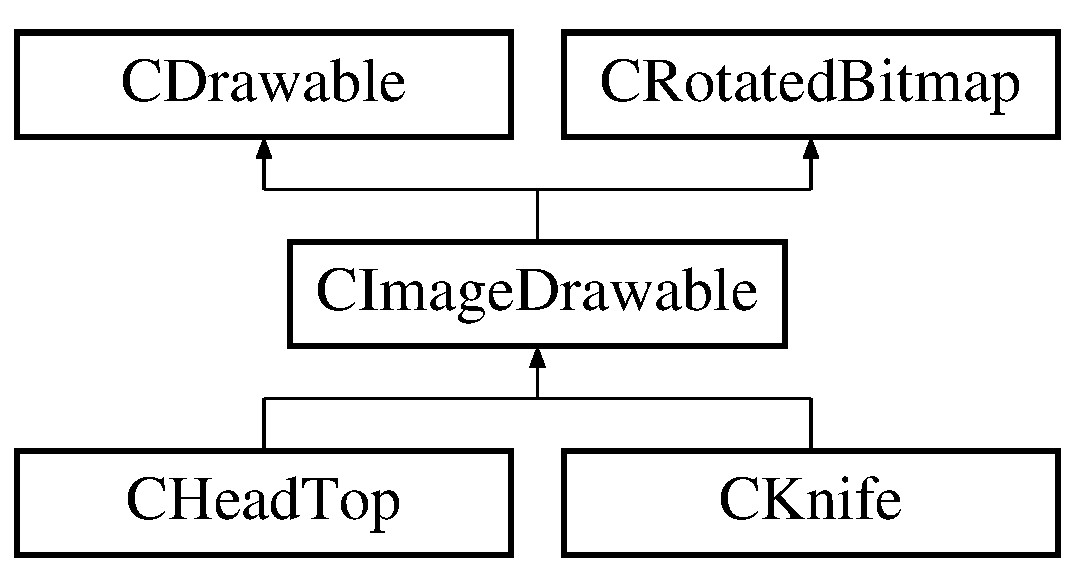
\includegraphics[height=3.000000cm]{class_c_image_drawable}
\end{center}
\end{figure}
\subsection*{Public Member Functions}
\begin{DoxyCompactItemize}
\item 
\hyperlink{class_c_image_drawable_a0a036788340edfd1765ae6a05cee31a0}{C\+Image\+Drawable} (const std\+::wstring \&name, const std\+::wstring \&filename)
\begin{DoxyCompactList}\small\item\em Constructor. \end{DoxyCompactList}\item 
\hypertarget{class_c_image_drawable_a0af067ad80ece0bea046dded19c5b9d4}{\hyperlink{class_c_image_drawable_a0af067ad80ece0bea046dded19c5b9d4}{C\+Image\+Drawable} ()=delete}\label{class_c_image_drawable_a0af067ad80ece0bea046dded19c5b9d4}

\begin{DoxyCompactList}\small\item\em Default constructor disabled. \end{DoxyCompactList}\item 
\hypertarget{class_c_image_drawable_a2955356238c638373d39ed99c5422cf3}{\hyperlink{class_c_image_drawable_a2955356238c638373d39ed99c5422cf3}{C\+Image\+Drawable} (const \hyperlink{class_c_image_drawable}{C\+Image\+Drawable} \&)=delete}\label{class_c_image_drawable_a2955356238c638373d39ed99c5422cf3}

\begin{DoxyCompactList}\small\item\em Copy constructor disabled. \end{DoxyCompactList}\item 
\hypertarget{class_c_image_drawable_a717129f6ce9e9fa5d9a512a85a33a8b1}{void \hyperlink{class_c_image_drawable_a717129f6ce9e9fa5d9a512a85a33a8b1}{operator=} (const \hyperlink{class_c_image_drawable}{C\+Image\+Drawable} \&)=delete}\label{class_c_image_drawable_a717129f6ce9e9fa5d9a512a85a33a8b1}

\begin{DoxyCompactList}\small\item\em Assignment operator disabled. \end{DoxyCompactList}\item 
virtual void \hyperlink{class_c_image_drawable_ada4d5d342230fbecb7169e4f3324ee52}{Draw} (Gdiplus\+::\+Graphics $\ast$graphics) override
\begin{DoxyCompactList}\small\item\em Draw the image drawable. \end{DoxyCompactList}\item 
virtual bool \hyperlink{class_c_image_drawable_a8aac5e64e309f1990e757f564dbcb8fd}{Hit\+Test} (Gdiplus\+::\+Point pos) override
\begin{DoxyCompactList}\small\item\em Test to see if we clicked on the image. \end{DoxyCompactList}\end{DoxyCompactItemize}
\subsection*{Additional Inherited Members}


\subsection{Detailed Description}
A drawable based on drawing a bitmap image. 

\subsection{Constructor \& Destructor Documentation}
\hypertarget{class_c_image_drawable_a0a036788340edfd1765ae6a05cee31a0}{\index{C\+Image\+Drawable@{C\+Image\+Drawable}!C\+Image\+Drawable@{C\+Image\+Drawable}}
\index{C\+Image\+Drawable@{C\+Image\+Drawable}!C\+Image\+Drawable@{C\+Image\+Drawable}}
\subsubsection[{C\+Image\+Drawable}]{\setlength{\rightskip}{0pt plus 5cm}C\+Image\+Drawable\+::\+C\+Image\+Drawable (
\begin{DoxyParamCaption}
\item[{const std\+::wstring \&}]{name, }
\item[{const std\+::wstring \&}]{filename}
\end{DoxyParamCaption}
)}}\label{class_c_image_drawable_a0a036788340edfd1765ae6a05cee31a0}


Constructor. 


\begin{DoxyParams}{Parameters}
{\em name} & The drawable name \\
\hline
{\em filename} & The filename for the image \\
\hline
\end{DoxyParams}


\subsection{Member Function Documentation}
\hypertarget{class_c_image_drawable_ada4d5d342230fbecb7169e4f3324ee52}{\index{C\+Image\+Drawable@{C\+Image\+Drawable}!Draw@{Draw}}
\index{Draw@{Draw}!C\+Image\+Drawable@{C\+Image\+Drawable}}
\subsubsection[{Draw}]{\setlength{\rightskip}{0pt plus 5cm}void C\+Image\+Drawable\+::\+Draw (
\begin{DoxyParamCaption}
\item[{Gdiplus\+::\+Graphics $\ast$}]{graphics}
\end{DoxyParamCaption}
)\hspace{0.3cm}{\ttfamily [override]}, {\ttfamily [virtual]}}}\label{class_c_image_drawable_ada4d5d342230fbecb7169e4f3324ee52}


Draw the image drawable. 


\begin{DoxyParams}{Parameters}
{\em graphics} & Graphics context to draw on \\
\hline
\end{DoxyParams}


Implements \hyperlink{class_c_drawable_a9b6a9920a75d88d9ae321997495eaec7}{C\+Drawable}.



Reimplemented in \hyperlink{class_c_head_top_aa77d9fa703079ee68a4e4e8e3c816932}{C\+Head\+Top}, and \hyperlink{class_c_knife_a71b0ee76740242e1e04f1f1500422ca3}{C\+Knife}.

\hypertarget{class_c_image_drawable_a8aac5e64e309f1990e757f564dbcb8fd}{\index{C\+Image\+Drawable@{C\+Image\+Drawable}!Hit\+Test@{Hit\+Test}}
\index{Hit\+Test@{Hit\+Test}!C\+Image\+Drawable@{C\+Image\+Drawable}}
\subsubsection[{Hit\+Test}]{\setlength{\rightskip}{0pt plus 5cm}bool C\+Image\+Drawable\+::\+Hit\+Test (
\begin{DoxyParamCaption}
\item[{Gdiplus\+::\+Point}]{pos}
\end{DoxyParamCaption}
)\hspace{0.3cm}{\ttfamily [override]}, {\ttfamily [virtual]}}}\label{class_c_image_drawable_a8aac5e64e309f1990e757f564dbcb8fd}


Test to see if we clicked on the image. 


\begin{DoxyParams}{Parameters}
{\em pos} & Position to test \\
\hline
\end{DoxyParams}
\begin{DoxyReturn}{Returns}
True if clicked on 
\end{DoxyReturn}


Implements \hyperlink{class_c_drawable_a43490aec87b1209bbf7441e3855f0874}{C\+Drawable}.



The documentation for this class was generated from the following files\+:\begin{DoxyCompactItemize}
\item 
\hyperlink{_image_drawable_8h}{Image\+Drawable.\+h}\item 
\hyperlink{_image_drawable_8cpp}{Image\+Drawable.\+cpp}\end{DoxyCompactItemize}

\hypertarget{class_c_knife}{\section{C\+Knife Class Reference}
\label{class_c_knife}\index{C\+Knife@{C\+Knife}}
}


Implemnet the knife for sparty.  




{\ttfamily \#include $<$Knife.\+h$>$}

Inheritance diagram for C\+Knife\+:\begin{figure}[H]
\begin{center}
\leavevmode
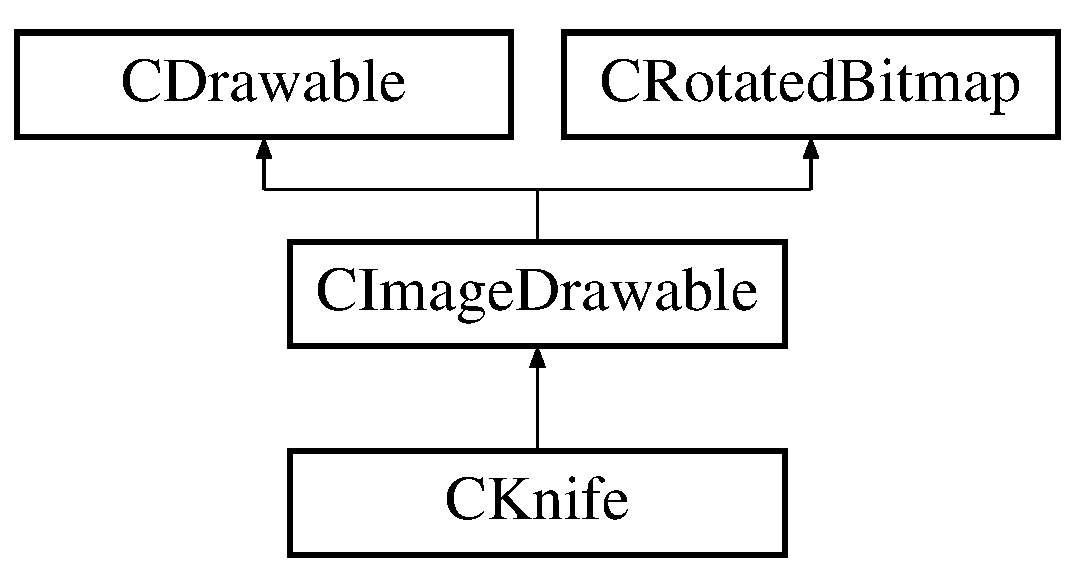
\includegraphics[height=3.000000cm]{class_c_knife}
\end{center}
\end{figure}
\subsection*{Public Member Functions}
\begin{DoxyCompactItemize}
\item 
\hyperlink{class_c_knife_a8f2311e0e0ecd4f79d1ed17d5aef14ae}{C\+Knife} (const std\+::wstring \&name, const std\+::wstring \&filename)
\begin{DoxyCompactList}\small\item\em Constructor for a knife object. \end{DoxyCompactList}\item 
\hypertarget{class_c_knife_a2d105884d8d86c62b3014649810d68a5}{\hyperlink{class_c_knife_a2d105884d8d86c62b3014649810d68a5}{C\+Knife} ()=delete}\label{class_c_knife_a2d105884d8d86c62b3014649810d68a5}

\begin{DoxyCompactList}\small\item\em Default constructor disabled. \end{DoxyCompactList}\item 
\hypertarget{class_c_knife_acba8b4484d6adc9965a9d3fdf84e24a1}{\hyperlink{class_c_knife_acba8b4484d6adc9965a9d3fdf84e24a1}{C\+Knife} (const \hyperlink{class_c_knife}{C\+Knife} \&)=delete}\label{class_c_knife_acba8b4484d6adc9965a9d3fdf84e24a1}

\begin{DoxyCompactList}\small\item\em Copy constructor disabled. \end{DoxyCompactList}\item 
\hypertarget{class_c_knife_a0ce92d419fa5e95a7ff16a956f5e4971}{void \hyperlink{class_c_knife_a0ce92d419fa5e95a7ff16a956f5e4971}{operator=} (const \hyperlink{class_c_knife}{C\+Knife} \&)=delete}\label{class_c_knife_a0ce92d419fa5e95a7ff16a956f5e4971}

\begin{DoxyCompactList}\small\item\em Assignment operator disabled. \end{DoxyCompactList}\item 
\hypertarget{class_c_knife_aee287cdbd992f49dbcfca75f6ed7cb0c}{\hyperlink{class_c_knife_aee287cdbd992f49dbcfca75f6ed7cb0c}{$\sim$\+C\+Knife} ()}\label{class_c_knife_aee287cdbd992f49dbcfca75f6ed7cb0c}

\begin{DoxyCompactList}\small\item\em Destructor. \end{DoxyCompactList}\item 
virtual bool \hyperlink{class_c_knife_a838e9409d22b1cc04d584abc611b65e6}{Is\+Movable} ()
\begin{DoxyCompactList}\small\item\em Is this drawable moveable? \end{DoxyCompactList}\item 
void \hyperlink{class_c_knife_a71b0ee76740242e1e04f1f1500422ca3}{Draw} (Gdiplus\+::\+Graphics $\ast$graphics)
\begin{DoxyCompactList}\small\item\em Draw the head. \end{DoxyCompactList}\item 
virtual void \hyperlink{class_c_knife_a1586c8502c39cd3032785d946a1f3f73}{Set\+Actor} (\hyperlink{class_c_actor}{C\+Actor} $\ast$actor) override
\begin{DoxyCompactList}\small\item\em Set the actor. This is where we set the channel name. \end{DoxyCompactList}\item 
virtual void \hyperlink{class_c_knife_a74c7de63a301d48c10b9dd0ad2c45735}{Set\+Timeline} (\hyperlink{class_c_timeline}{C\+Timeline} $\ast$timeline) override
\begin{DoxyCompactList}\small\item\em Set the timeline. The tells the channel the timeline. \end{DoxyCompactList}\item 
\hypertarget{class_c_knife_ab2631848d790223266fb0ea6b8540d34}{virtual void \hyperlink{class_c_knife_ab2631848d790223266fb0ea6b8540d34}{Set\+Keyframe} () override}\label{class_c_knife_ab2631848d790223266fb0ea6b8540d34}

\begin{DoxyCompactList}\small\item\em Set the keyframe based on the current status. \end{DoxyCompactList}\item 
\hypertarget{class_c_knife_ae68af382999c5ed27feae4e210a2ff2f}{virtual void \hyperlink{class_c_knife_ae68af382999c5ed27feae4e210a2ff2f}{Get\+Keyframe} () override}\label{class_c_knife_ae68af382999c5ed27feae4e210a2ff2f}

\begin{DoxyCompactList}\small\item\em Get the current channel from the animation system. \end{DoxyCompactList}\end{DoxyCompactItemize}
\subsection*{Additional Inherited Members}


\subsection{Detailed Description}
Implemnet the knife for sparty. 

\subsection{Constructor \& Destructor Documentation}
\hypertarget{class_c_knife_a8f2311e0e0ecd4f79d1ed17d5aef14ae}{\index{C\+Knife@{C\+Knife}!C\+Knife@{C\+Knife}}
\index{C\+Knife@{C\+Knife}!C\+Knife@{C\+Knife}}
\subsubsection[{C\+Knife}]{\setlength{\rightskip}{0pt plus 5cm}C\+Knife\+::\+C\+Knife (
\begin{DoxyParamCaption}
\item[{const std\+::wstring \&}]{name, }
\item[{const std\+::wstring \&}]{filename}
\end{DoxyParamCaption}
)}}\label{class_c_knife_a8f2311e0e0ecd4f79d1ed17d5aef14ae}


Constructor for a knife object. 


\begin{DoxyParams}{Parameters}
{\em name} & The drawable name to use \\
\hline
{\em filename} & The filename for the image to use \\
\hline
\end{DoxyParams}


\subsection{Member Function Documentation}
\hypertarget{class_c_knife_a71b0ee76740242e1e04f1f1500422ca3}{\index{C\+Knife@{C\+Knife}!Draw@{Draw}}
\index{Draw@{Draw}!C\+Knife@{C\+Knife}}
\subsubsection[{Draw}]{\setlength{\rightskip}{0pt plus 5cm}void C\+Knife\+::\+Draw (
\begin{DoxyParamCaption}
\item[{Gdiplus\+::\+Graphics $\ast$}]{graphics}
\end{DoxyParamCaption}
)\hspace{0.3cm}{\ttfamily [virtual]}}}\label{class_c_knife_a71b0ee76740242e1e04f1f1500422ca3}


Draw the head. 


\begin{DoxyParams}{Parameters}
{\em graphics} & Graphics context to draw on \\
\hline
\end{DoxyParams}


Reimplemented from \hyperlink{class_c_image_drawable_ada4d5d342230fbecb7169e4f3324ee52}{C\+Image\+Drawable}.

\hypertarget{class_c_knife_a838e9409d22b1cc04d584abc611b65e6}{\index{C\+Knife@{C\+Knife}!Is\+Movable@{Is\+Movable}}
\index{Is\+Movable@{Is\+Movable}!C\+Knife@{C\+Knife}}
\subsubsection[{Is\+Movable}]{\setlength{\rightskip}{0pt plus 5cm}virtual bool C\+Knife\+::\+Is\+Movable (
\begin{DoxyParamCaption}
{}
\end{DoxyParamCaption}
)\hspace{0.3cm}{\ttfamily [inline]}, {\ttfamily [virtual]}}}\label{class_c_knife_a838e9409d22b1cc04d584abc611b65e6}


Is this drawable moveable? 

\begin{DoxyReturn}{Returns}
true 
\end{DoxyReturn}


Reimplemented from \hyperlink{class_c_drawable_ac9f03cfc58aed75fb52cd69c71e7b6e0}{C\+Drawable}.

\hypertarget{class_c_knife_a1586c8502c39cd3032785d946a1f3f73}{\index{C\+Knife@{C\+Knife}!Set\+Actor@{Set\+Actor}}
\index{Set\+Actor@{Set\+Actor}!C\+Knife@{C\+Knife}}
\subsubsection[{Set\+Actor}]{\setlength{\rightskip}{0pt plus 5cm}void C\+Knife\+::\+Set\+Actor (
\begin{DoxyParamCaption}
\item[{{\bf C\+Actor} $\ast$}]{actor}
\end{DoxyParamCaption}
)\hspace{0.3cm}{\ttfamily [override]}, {\ttfamily [virtual]}}}\label{class_c_knife_a1586c8502c39cd3032785d946a1f3f73}


Set the actor. This is where we set the channel name. 


\begin{DoxyParams}{Parameters}
{\em actor} & Actor to set \\
\hline
\end{DoxyParams}


Reimplemented from \hyperlink{class_c_drawable_a86762c6e220d9f502c6ccf9baf1135ac}{C\+Drawable}.

\hypertarget{class_c_knife_a74c7de63a301d48c10b9dd0ad2c45735}{\index{C\+Knife@{C\+Knife}!Set\+Timeline@{Set\+Timeline}}
\index{Set\+Timeline@{Set\+Timeline}!C\+Knife@{C\+Knife}}
\subsubsection[{Set\+Timeline}]{\setlength{\rightskip}{0pt plus 5cm}void C\+Knife\+::\+Set\+Timeline (
\begin{DoxyParamCaption}
\item[{{\bf C\+Timeline} $\ast$}]{timeline}
\end{DoxyParamCaption}
)\hspace{0.3cm}{\ttfamily [override]}, {\ttfamily [virtual]}}}\label{class_c_knife_a74c7de63a301d48c10b9dd0ad2c45735}


Set the timeline. The tells the channel the timeline. 


\begin{DoxyParams}{Parameters}
{\em timeline} & Timeline to set \\
\hline
\end{DoxyParams}


Reimplemented from \hyperlink{class_c_drawable_a479df46ae298bf716d96b05b1ba6e529}{C\+Drawable}.



The documentation for this class was generated from the following files\+:\begin{DoxyCompactItemize}
\item 
\hyperlink{_knife_8h}{Knife.\+h}\item 
\hyperlink{_knife_8cpp}{Knife.\+cpp}\end{DoxyCompactItemize}

\hypertarget{class_c_linked_list}{\section{C\+Linked\+List Class Reference}
\label{class_c_linked_list}\index{C\+Linked\+List@{C\+Linked\+List}}
}


The linked calss to store the snow flakes.  




{\ttfamily \#include $<$Linked\+List.\+h$>$}

\subsection*{Public Member Functions}
\begin{DoxyCompactItemize}
\item 
\hypertarget{class_c_linked_list_a1acc364e288b1fd8deef87405d55eb8b}{\hyperlink{class_c_linked_list_a1acc364e288b1fd8deef87405d55eb8b}{C\+Linked\+List} ()}\label{class_c_linked_list_a1acc364e288b1fd8deef87405d55eb8b}

\begin{DoxyCompactList}\small\item\em Constructor. \end{DoxyCompactList}\item 
\hypertarget{class_c_linked_list_a485e9d04a818f41bc49b8190c7eab5ab}{\hyperlink{class_c_linked_list_a485e9d04a818f41bc49b8190c7eab5ab}{$\sim$\+C\+Linked\+List} ()}\label{class_c_linked_list_a485e9d04a818f41bc49b8190c7eab5ab}

\begin{DoxyCompactList}\small\item\em Destructor. \end{DoxyCompactList}\item 
void \hyperlink{class_c_linked_list_a99ab91eab972887ff91d11cc23550391}{Insert} (std\+::shared\+\_\+ptr$<$ \hyperlink{class_c_snowflake}{C\+Snowflake} $>$ flake)
\begin{DoxyCompactList}\small\item\em Insert a snowfalke to the tail of linked list. \end{DoxyCompactList}\item 
std\+::shared\+\_\+ptr$<$ \hyperlink{class_c_snowflake}{C\+Snowflake} $>$ \hyperlink{class_c_linked_list_af26de4eaa8a0c7df65be6a458e6224c9}{Popfront} ()
\begin{DoxyCompactList}\small\item\em Popfront the first snowflake in the list and return it. \end{DoxyCompactList}\item 
\hypertarget{class_c_linked_list_a715d68d55b85aa65f7ca0ad2e1970776}{void \hyperlink{class_c_linked_list_a715d68d55b85aa65f7ca0ad2e1970776}{Remove} (std\+::shared\+\_\+ptr$<$ \hyperlink{class_c_snowflake}{C\+Snowflake} $>$ temp)}\label{class_c_linked_list_a715d68d55b85aa65f7ca0ad2e1970776}

\begin{DoxyCompactList}\small\item\em Remove a certain point from the linked list. \end{DoxyCompactList}\item 
std\+::shared\+\_\+ptr$<$ \hyperlink{class_c_snowflake}{C\+Snowflake} $>$ \hyperlink{class_c_linked_list_a56b88a4740720062da3d9dd0389bbc1d}{Get\+Head} ()
\begin{DoxyCompactList}\small\item\em Get the head of the linked list. \end{DoxyCompactList}\item 
std\+::shared\+\_\+ptr$<$ \hyperlink{class_c_snowflake}{C\+Snowflake} $>$ \hyperlink{class_c_linked_list_a14ae4d2fe8f2d8eab0fdf9a8831b2063}{Get\+Tail} ()
\begin{DoxyCompactList}\small\item\em Get the tail of the linked list. \end{DoxyCompactList}\end{DoxyCompactItemize}


\subsection{Detailed Description}
The linked calss to store the snow flakes. 

\subsection{Member Function Documentation}
\hypertarget{class_c_linked_list_a56b88a4740720062da3d9dd0389bbc1d}{\index{C\+Linked\+List@{C\+Linked\+List}!Get\+Head@{Get\+Head}}
\index{Get\+Head@{Get\+Head}!C\+Linked\+List@{C\+Linked\+List}}
\subsubsection[{Get\+Head}]{\setlength{\rightskip}{0pt plus 5cm}std\+::shared\+\_\+ptr$<${\bf C\+Snowflake}$>$ C\+Linked\+List\+::\+Get\+Head (
\begin{DoxyParamCaption}
{}
\end{DoxyParamCaption}
)\hspace{0.3cm}{\ttfamily [inline]}}}\label{class_c_linked_list_a56b88a4740720062da3d9dd0389bbc1d}


Get the head of the linked list. 

\begin{DoxyReturn}{Returns}
the header pointer 
\end{DoxyReturn}
\hypertarget{class_c_linked_list_a14ae4d2fe8f2d8eab0fdf9a8831b2063}{\index{C\+Linked\+List@{C\+Linked\+List}!Get\+Tail@{Get\+Tail}}
\index{Get\+Tail@{Get\+Tail}!C\+Linked\+List@{C\+Linked\+List}}
\subsubsection[{Get\+Tail}]{\setlength{\rightskip}{0pt plus 5cm}std\+::shared\+\_\+ptr$<${\bf C\+Snowflake}$>$ C\+Linked\+List\+::\+Get\+Tail (
\begin{DoxyParamCaption}
{}
\end{DoxyParamCaption}
)\hspace{0.3cm}{\ttfamily [inline]}}}\label{class_c_linked_list_a14ae4d2fe8f2d8eab0fdf9a8831b2063}


Get the tail of the linked list. 

\begin{DoxyReturn}{Returns}
the tail pointer 
\end{DoxyReturn}
\hypertarget{class_c_linked_list_a99ab91eab972887ff91d11cc23550391}{\index{C\+Linked\+List@{C\+Linked\+List}!Insert@{Insert}}
\index{Insert@{Insert}!C\+Linked\+List@{C\+Linked\+List}}
\subsubsection[{Insert}]{\setlength{\rightskip}{0pt plus 5cm}void C\+Linked\+List\+::\+Insert (
\begin{DoxyParamCaption}
\item[{std\+::shared\+\_\+ptr$<$ {\bf C\+Snowflake} $>$}]{flake}
\end{DoxyParamCaption}
)}}\label{class_c_linked_list_a99ab91eab972887ff91d11cc23550391}


Insert a snowfalke to the tail of linked list. 


\begin{DoxyParams}{Parameters}
{\em flake} & the Snowflake to insert to the end \\
\hline
\end{DoxyParams}
\hypertarget{class_c_linked_list_af26de4eaa8a0c7df65be6a458e6224c9}{\index{C\+Linked\+List@{C\+Linked\+List}!Popfront@{Popfront}}
\index{Popfront@{Popfront}!C\+Linked\+List@{C\+Linked\+List}}
\subsubsection[{Popfront}]{\setlength{\rightskip}{0pt plus 5cm}std\+::shared\+\_\+ptr$<$ {\bf C\+Snowflake} $>$ C\+Linked\+List\+::\+Popfront (
\begin{DoxyParamCaption}
{}
\end{DoxyParamCaption}
)}}\label{class_c_linked_list_af26de4eaa8a0c7df65be6a458e6224c9}


Popfront the first snowflake in the list and return it. 

\begin{DoxyReturn}{Returns}
the snowfleak pop out 
\end{DoxyReturn}


The documentation for this class was generated from the following files\+:\begin{DoxyCompactItemize}
\item 
\hyperlink{_linked_list_8h}{Linked\+List.\+h}\item 
\hyperlink{_linked_list_8cpp}{Linked\+List.\+cpp}\end{DoxyCompactItemize}

\hypertarget{class_c_main_frame}{\section{C\+Main\+Frame Class Reference}
\label{class_c_main_frame}\index{C\+Main\+Frame@{C\+Main\+Frame}}
}


Program main frame.  




{\ttfamily \#include $<$Main\+Frm.\+h$>$}

Inheritance diagram for C\+Main\+Frame\+:\begin{figure}[H]
\begin{center}
\leavevmode
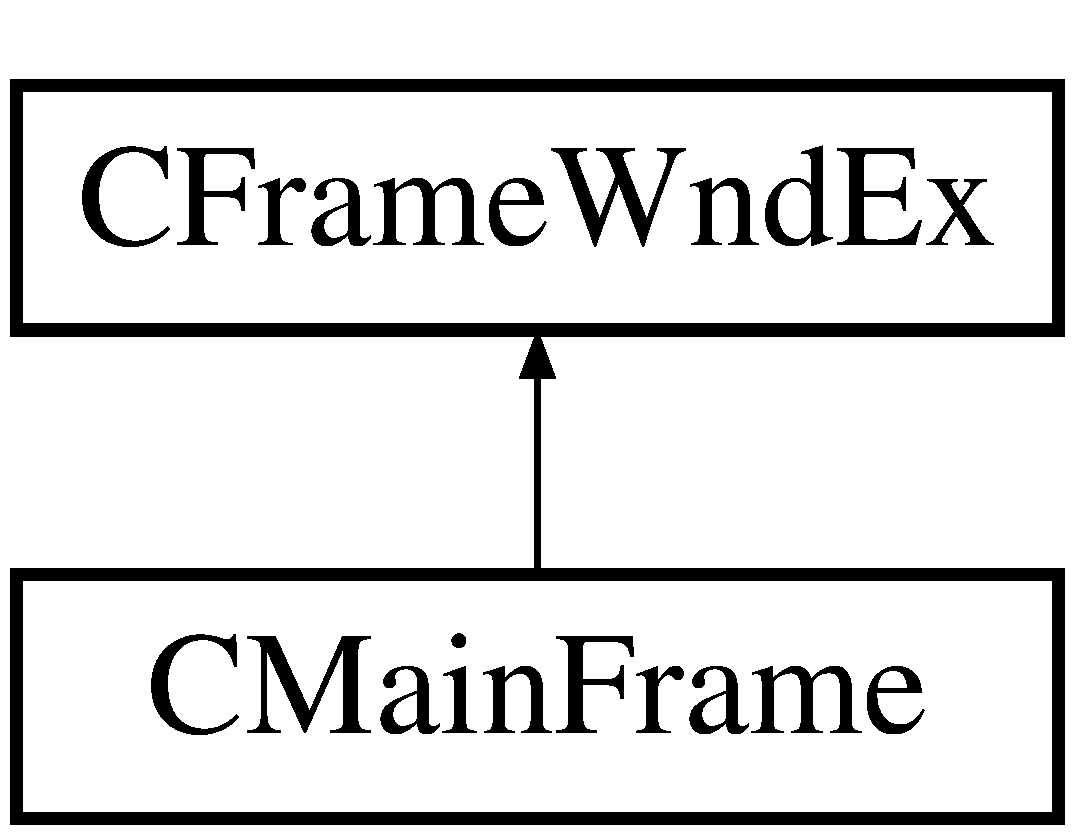
\includegraphics[height=2.000000cm]{class_c_main_frame}
\end{center}
\end{figure}
\subsection*{Public Types}
\begin{DoxyCompactItemize}
\item 
\hypertarget{class_c_main_frame_a89722c82d82f95a761772a8dd9755b7b}{enum \hyperlink{class_c_main_frame_a89722c82d82f95a761772a8dd9755b7b}{Motion\+Modes} \{ {\bfseries Move}, 
{\bfseries Rotate}
 \}}\label{class_c_main_frame_a89722c82d82f95a761772a8dd9755b7b}

\begin{DoxyCompactList}\small\item\em Enumerations for the possible manipulation modes. \end{DoxyCompactList}\end{DoxyCompactItemize}
\subsection*{Public Member Functions}
\begin{DoxyCompactItemize}
\item 
\hypertarget{class_c_main_frame_af3e997aeae4148d2aaa4a1e1ae7bdd53}{\hyperlink{class_c_main_frame_af3e997aeae4148d2aaa4a1e1ae7bdd53}{C\+Main\+Frame} ()}\label{class_c_main_frame_af3e997aeae4148d2aaa4a1e1ae7bdd53}

\begin{DoxyCompactList}\small\item\em Constructor. \end{DoxyCompactList}\item 
\hyperlink{class_c_main_frame_a89722c82d82f95a761772a8dd9755b7b}{Motion\+Modes} \hyperlink{class_c_main_frame_a76c571ab75752dba8049e08f5e4ac920}{Get\+Mode} () const 
\begin{DoxyCompactList}\small\item\em The selected manipulation mode. \end{DoxyCompactList}\item 
\hypertarget{class_c_main_frame_a549bf677c955c2898c3c683321633c16}{virtual B\+O\+O\+L {\bfseries Pre\+Create\+Window} (C\+R\+E\+A\+T\+E\+S\+T\+R\+U\+C\+T \&cs)}\label{class_c_main_frame_a549bf677c955c2898c3c683321633c16}

\item 
\hypertarget{class_c_main_frame_ade959eb0bab719bf06bb9b18ee407101}{virtual B\+O\+O\+L {\bfseries On\+Cmd\+Msg} (U\+I\+N\+T n\+I\+D, int n\+Code, void $\ast$p\+Extra, A\+F\+X\+\_\+\+C\+M\+D\+H\+A\+N\+D\+L\+E\+R\+I\+N\+F\+O $\ast$p\+Handler\+Info)}\label{class_c_main_frame_ade959eb0bab719bf06bb9b18ee407101}

\item 
\hypertarget{class_c_main_frame_a8ae555f23fdf97edb4feb4d3e1bfa4ee}{virtual \hyperlink{class_c_main_frame_a8ae555f23fdf97edb4feb4d3e1bfa4ee}{$\sim$\+C\+Main\+Frame} ()}\label{class_c_main_frame_a8ae555f23fdf97edb4feb4d3e1bfa4ee}

\begin{DoxyCompactList}\small\item\em Destructor. \end{DoxyCompactList}\item 
afx\+\_\+msg void \hyperlink{class_c_main_frame_adf171bf1f2c6f10cc85dbe8db3fc93f7}{On\+Size} (U\+I\+N\+T n\+Type, int cx, int cy)
\begin{DoxyCompactList}\small\item\em Handle a Size request from Windows. \end{DoxyCompactList}\item 
afx\+\_\+msg B\+O\+O\+L \hyperlink{class_c_main_frame_a53a97f2229c5765329b2b59a21a54b0d}{On\+Erase\+Bkgnd} (C\+D\+C $\ast$p\+D\+C)
\begin{DoxyCompactList}\small\item\em Called to erase the background. Disabled so we don't get flicker. \end{DoxyCompactList}\item 
\hypertarget{class_c_main_frame_af07c2610f9f5631e7eb7374d10d5fdd3}{afx\+\_\+msg void \hyperlink{class_c_main_frame_af07c2610f9f5631e7eb7374d10d5fdd3}{On\+Edit\+Move} ()}\label{class_c_main_frame_af07c2610f9f5631e7eb7374d10d5fdd3}

\begin{DoxyCompactList}\small\item\em Handle the Edit$>$Mode menu option. \end{DoxyCompactList}\item 
afx\+\_\+msg void \hyperlink{class_c_main_frame_aadc40c4ab290da2368f6b87443f5ffbc}{On\+Update\+Edit\+Move} (C\+Cmd\+U\+I $\ast$p\+Cmd\+U\+I)
\begin{DoxyCompactList}\small\item\em Update the menu for Edit$>$Move. \end{DoxyCompactList}\item 
\hypertarget{class_c_main_frame_a00f10667f35de1fa6693c1bea941d878}{afx\+\_\+msg void \hyperlink{class_c_main_frame_a00f10667f35de1fa6693c1bea941d878}{On\+Edit\+Rotate} ()}\label{class_c_main_frame_a00f10667f35de1fa6693c1bea941d878}

\begin{DoxyCompactList}\small\item\em Handle the Edit$>$Rotate menu option. \end{DoxyCompactList}\item 
afx\+\_\+msg void \hyperlink{class_c_main_frame_af098b8129775d1b5fb47fcaaabce8c01}{On\+Update\+Edit\+Rotate} (C\+Cmd\+U\+I $\ast$p\+Cmd\+U\+I)
\begin{DoxyCompactList}\small\item\em Update the menu for Edit$>$Rotate. \end{DoxyCompactList}\item 
\hypertarget{class_c_main_frame_a73eb391d84e16eb934f2f66c1500af25}{afx\+\_\+msg void \hyperlink{class_c_main_frame_a73eb391d84e16eb934f2f66c1500af25}{On\+Edit\+Timelineproperties} ()}\label{class_c_main_frame_a73eb391d84e16eb934f2f66c1500af25}

\begin{DoxyCompactList}\small\item\em Handle the Edit/\+Timeline Properties menu option. \end{DoxyCompactList}\item 
\hypertarget{class_c_main_frame_a5210794fc4f5e85a455340a61b25f0c5}{afx\+\_\+msg void \hyperlink{class_c_main_frame_a5210794fc4f5e85a455340a61b25f0c5}{On\+Edit\+Textbubbleforsparty} ()}\label{class_c_main_frame_a5210794fc4f5e85a455340a61b25f0c5}

\begin{DoxyCompactList}\small\item\em Handle the Text Bubble for Sparty Menu option. \end{DoxyCompactList}\item 
\hypertarget{class_c_main_frame_a8dd4bfbe4d04dc6521680afca02110be}{afx\+\_\+msg void \hyperlink{class_c_main_frame_a8dd4bfbe4d04dc6521680afca02110be}{On\+Edit\+Textbubbleforharold} ()}\label{class_c_main_frame_a8dd4bfbe4d04dc6521680afca02110be}

\begin{DoxyCompactList}\small\item\em Handle the Text Bubble for H\+A\+R\+O\+L\+D Menu option. \end{DoxyCompactList}\item 
\hypertarget{class_c_main_frame_ac3d4e57ed47cf13a028f53ba141f329a}{afx\+\_\+msg void \hyperlink{class_c_main_frame_ac3d4e57ed47cf13a028f53ba141f329a}{On\+Play\+Play} ()}\label{class_c_main_frame_ac3d4e57ed47cf13a028f53ba141f329a}

\begin{DoxyCompactList}\small\item\em Handle the Play Menu Option. \end{DoxyCompactList}\item 
afx\+\_\+msg void \hyperlink{class_c_main_frame_a244f55f3c149650ade8e7f66e599897b}{On\+Timer} (U\+I\+N\+T\+\_\+\+P\+T\+R n\+I\+D\+Event)
\begin{DoxyCompactList}\small\item\em The timer to track the time on play. \end{DoxyCompactList}\item 
\hypertarget{class_c_main_frame_a9fba7b1e608163dddb6dd5e18c30aa02}{afx\+\_\+msg void \hyperlink{class_c_main_frame_a9fba7b1e608163dddb6dd5e18c30aa02}{On\+Play\+Playfrombeginnning} ()}\label{class_c_main_frame_a9fba7b1e608163dddb6dd5e18c30aa02}

\begin{DoxyCompactList}\small\item\em Handle play from beginning menu option. \end{DoxyCompactList}\item 
\hypertarget{class_c_main_frame_a75fade7a5583c8019e2f98d9196509bf}{afx\+\_\+msg void \hyperlink{class_c_main_frame_a75fade7a5583c8019e2f98d9196509bf}{On\+Play\+Stop} ()}\label{class_c_main_frame_a75fade7a5583c8019e2f98d9196509bf}

\begin{DoxyCompactList}\small\item\em Handle stop the play menu option. \end{DoxyCompactList}\end{DoxyCompactItemize}
\subsection*{Protected Member Functions}
\begin{DoxyCompactItemize}
\item 
\hypertarget{class_c_main_frame_a48666466fd37412fcaeff75c3b12e0ed}{afx\+\_\+msg int {\bfseries On\+Create} (L\+P\+C\+R\+E\+A\+T\+E\+S\+T\+R\+U\+C\+T lp\+Create\+Struct)}\label{class_c_main_frame_a48666466fd37412fcaeff75c3b12e0ed}

\item 
\hypertarget{class_c_main_frame_adc353a3d1fc497fbc009b6d9e6914a82}{afx\+\_\+msg void {\bfseries On\+Set\+Focus} (C\+Wnd $\ast$p\+Old\+Wnd)}\label{class_c_main_frame_adc353a3d1fc497fbc009b6d9e6914a82}

\item 
\hypertarget{class_c_main_frame_ac863d694fd3637d492ef97396defbd8e}{virtual B\+O\+O\+L {\bfseries On\+Create\+Client} (L\+P\+C\+R\+E\+A\+T\+E\+S\+T\+R\+U\+C\+T lpcs, C\+Create\+Context $\ast$p\+Context)}\label{class_c_main_frame_ac863d694fd3637d492ef97396defbd8e}

\end{DoxyCompactItemize}
\subsection*{Protected Attributes}
\begin{DoxyCompactItemize}
\item 
\hypertarget{class_c_main_frame_ac8558942627d1502b5095e736840a1f3}{C\+M\+F\+C\+Tool\+Bar {\bfseries m\+\_\+wnd\+Tool\+Bar}}\label{class_c_main_frame_ac8558942627d1502b5095e736840a1f3}

\item 
\hypertarget{class_c_main_frame_a5842bded00e9137fbbf77343b99863be}{C\+M\+F\+C\+Status\+Bar {\bfseries m\+\_\+wnd\+Status\+Bar}}\label{class_c_main_frame_a5842bded00e9137fbbf77343b99863be}

\item 
\hypertarget{class_c_main_frame_a1d68466db594c4bebf41f707bc0a0647}{C\+Splitter\+Wnd {\bfseries m\+Wnd\+Splitter}}\label{class_c_main_frame_a1d68466db594c4bebf41f707bc0a0647}

\end{DoxyCompactItemize}


\subsection{Detailed Description}
Program main frame. 

\subsection{Member Function Documentation}
\hypertarget{class_c_main_frame_a76c571ab75752dba8049e08f5e4ac920}{\index{C\+Main\+Frame@{C\+Main\+Frame}!Get\+Mode@{Get\+Mode}}
\index{Get\+Mode@{Get\+Mode}!C\+Main\+Frame@{C\+Main\+Frame}}
\subsubsection[{Get\+Mode}]{\setlength{\rightskip}{0pt plus 5cm}{\bf Motion\+Modes} C\+Main\+Frame\+::\+Get\+Mode (
\begin{DoxyParamCaption}
{}
\end{DoxyParamCaption}
) const\hspace{0.3cm}{\ttfamily [inline]}}}\label{class_c_main_frame_a76c571ab75752dba8049e08f5e4ac920}


The selected manipulation mode. 

\begin{DoxyReturn}{Returns}
Currently selected manipulation mode 
\end{DoxyReturn}
\hypertarget{class_c_main_frame_a53a97f2229c5765329b2b59a21a54b0d}{\index{C\+Main\+Frame@{C\+Main\+Frame}!On\+Erase\+Bkgnd@{On\+Erase\+Bkgnd}}
\index{On\+Erase\+Bkgnd@{On\+Erase\+Bkgnd}!C\+Main\+Frame@{C\+Main\+Frame}}
\subsubsection[{On\+Erase\+Bkgnd}]{\setlength{\rightskip}{0pt plus 5cm}B\+O\+O\+L C\+Main\+Frame\+::\+On\+Erase\+Bkgnd (
\begin{DoxyParamCaption}
\item[{C\+D\+C $\ast$}]{p\+D\+C}
\end{DoxyParamCaption}
)}}\label{class_c_main_frame_a53a97f2229c5765329b2b59a21a54b0d}


Called to erase the background. Disabled so we don't get flicker. 


\begin{DoxyParams}{Parameters}
{\em p\+D\+C} & A device context \\
\hline
\end{DoxyParams}
\begin{DoxyReturn}{Returns}
F\+A\+L\+S\+E 
\end{DoxyReturn}
\hypertarget{class_c_main_frame_adf171bf1f2c6f10cc85dbe8db3fc93f7}{\index{C\+Main\+Frame@{C\+Main\+Frame}!On\+Size@{On\+Size}}
\index{On\+Size@{On\+Size}!C\+Main\+Frame@{C\+Main\+Frame}}
\subsubsection[{On\+Size}]{\setlength{\rightskip}{0pt plus 5cm}void C\+Main\+Frame\+::\+On\+Size (
\begin{DoxyParamCaption}
\item[{U\+I\+N\+T}]{n\+Type, }
\item[{int}]{cx, }
\item[{int}]{cy}
\end{DoxyParamCaption}
)}}\label{class_c_main_frame_adf171bf1f2c6f10cc85dbe8db3fc93f7}


Handle a Size request from Windows. 

This function ensures the child windows are the correct size on the screen after the main window is resized 
\begin{DoxyParams}{Parameters}
{\em n\+Type} & Type of resizing message \\
\hline
{\em cx} & The new width \\
\hline
{\em cy} & The new height \\
\hline
\end{DoxyParams}
\hypertarget{class_c_main_frame_a244f55f3c149650ade8e7f66e599897b}{\index{C\+Main\+Frame@{C\+Main\+Frame}!On\+Timer@{On\+Timer}}
\index{On\+Timer@{On\+Timer}!C\+Main\+Frame@{C\+Main\+Frame}}
\subsubsection[{On\+Timer}]{\setlength{\rightskip}{0pt plus 5cm}void C\+Main\+Frame\+::\+On\+Timer (
\begin{DoxyParamCaption}
\item[{U\+I\+N\+T\+\_\+\+P\+T\+R}]{n\+I\+D\+Event}
\end{DoxyParamCaption}
)}}\label{class_c_main_frame_a244f55f3c149650ade8e7f66e599897b}


The timer to track the time on play. 


\begin{DoxyParams}{Parameters}
{\em n\+I\+D\+Event} & \\
\hline
\end{DoxyParams}
\hypertarget{class_c_main_frame_aadc40c4ab290da2368f6b87443f5ffbc}{\index{C\+Main\+Frame@{C\+Main\+Frame}!On\+Update\+Edit\+Move@{On\+Update\+Edit\+Move}}
\index{On\+Update\+Edit\+Move@{On\+Update\+Edit\+Move}!C\+Main\+Frame@{C\+Main\+Frame}}
\subsubsection[{On\+Update\+Edit\+Move}]{\setlength{\rightskip}{0pt plus 5cm}void C\+Main\+Frame\+::\+On\+Update\+Edit\+Move (
\begin{DoxyParamCaption}
\item[{C\+Cmd\+U\+I $\ast$}]{p\+Cmd\+U\+I}
\end{DoxyParamCaption}
)}}\label{class_c_main_frame_aadc40c4ab290da2368f6b87443f5ffbc}


Update the menu for Edit$>$Move. 


\begin{DoxyParams}{Parameters}
{\em p\+Cmd\+U\+I} & The pointer to the control user interface \\
\hline
\end{DoxyParams}
\hypertarget{class_c_main_frame_af098b8129775d1b5fb47fcaaabce8c01}{\index{C\+Main\+Frame@{C\+Main\+Frame}!On\+Update\+Edit\+Rotate@{On\+Update\+Edit\+Rotate}}
\index{On\+Update\+Edit\+Rotate@{On\+Update\+Edit\+Rotate}!C\+Main\+Frame@{C\+Main\+Frame}}
\subsubsection[{On\+Update\+Edit\+Rotate}]{\setlength{\rightskip}{0pt plus 5cm}void C\+Main\+Frame\+::\+On\+Update\+Edit\+Rotate (
\begin{DoxyParamCaption}
\item[{C\+Cmd\+U\+I $\ast$}]{p\+Cmd\+U\+I}
\end{DoxyParamCaption}
)}}\label{class_c_main_frame_af098b8129775d1b5fb47fcaaabce8c01}


Update the menu for Edit$>$Rotate. 


\begin{DoxyParams}{Parameters}
{\em p\+Cmd\+U\+I} & The pointer to the control user interface \\
\hline
\end{DoxyParams}


The documentation for this class was generated from the following files\+:\begin{DoxyCompactItemize}
\item 
\hyperlink{_main_frm_8h}{Main\+Frm.\+h}\item 
\hyperlink{_main_frm_8cpp}{Main\+Frm.\+cpp}\end{DoxyCompactItemize}

\hypertarget{class_c_particle_system}{\section{C\+Particle\+System Class Reference}
\label{class_c_particle_system}\index{C\+Particle\+System@{C\+Particle\+System}}
}


The Particle\+System to implement the snow draw and update.  




{\ttfamily \#include $<$Particle\+System.\+h$>$}

\subsection*{Public Member Functions}
\begin{DoxyCompactItemize}
\item 
\hypertarget{class_c_particle_system_aeadc49bba6ac1391e8c0e8a2fa5b4f41}{\hyperlink{class_c_particle_system_aeadc49bba6ac1391e8c0e8a2fa5b4f41}{C\+Particle\+System} ()}\label{class_c_particle_system_aeadc49bba6ac1391e8c0e8a2fa5b4f41}

\begin{DoxyCompactList}\small\item\em Constructor. \end{DoxyCompactList}\item 
\hypertarget{class_c_particle_system_a1e46a5f93ae2f437e5d6b3c4b6305f80}{\hyperlink{class_c_particle_system_a1e46a5f93ae2f437e5d6b3c4b6305f80}{C\+Particle\+System} (const \hyperlink{class_c_particle_system}{C\+Particle\+System} \&)=delete}\label{class_c_particle_system_a1e46a5f93ae2f437e5d6b3c4b6305f80}

\begin{DoxyCompactList}\small\item\em Copy constructor disabled. \end{DoxyCompactList}\item 
\hypertarget{class_c_particle_system_a60636bbc9ceff92f1a89b4d7412eccdf}{void \hyperlink{class_c_particle_system_a60636bbc9ceff92f1a89b4d7412eccdf}{operator=} (const \hyperlink{class_c_particle_system}{C\+Particle\+System} \&)=delete}\label{class_c_particle_system_a60636bbc9ceff92f1a89b4d7412eccdf}

\begin{DoxyCompactList}\small\item\em Assignment operator disabled. \end{DoxyCompactList}\item 
\hypertarget{class_c_particle_system_aa73fea125a7e06b0cdfe622af9fdcb6b}{\hyperlink{class_c_particle_system_aa73fea125a7e06b0cdfe622af9fdcb6b}{$\sim$\+C\+Particle\+System} ()}\label{class_c_particle_system_aa73fea125a7e06b0cdfe622af9fdcb6b}

\begin{DoxyCompactList}\small\item\em Destructor. \end{DoxyCompactList}\item 
void \hyperlink{class_c_particle_system_a88c6b477ef797e66bc3407b55763cbe1}{Draw} (Gdiplus\+::\+Graphics $\ast$graphics, Gdiplus\+::\+Solid\+Brush $\ast$brush)
\begin{DoxyCompactList}\small\item\em Draw the snowflakes in the linked list. \end{DoxyCompactList}\item 
void \hyperlink{class_c_particle_system_a5e7c19dbfea60bb422e98ae79aa56692}{Update} (double elapsed)
\begin{DoxyCompactList}\small\item\em The update function to update each fleak in the linked list. \end{DoxyCompactList}\item 
\hypertarget{class_c_particle_system_a1d402912cabfb3914f42ce3273e8b9e4}{void \hyperlink{class_c_particle_system_a1d402912cabfb3914f42ce3273e8b9e4}{Set\+Width} (int w)}\label{class_c_particle_system_a1d402912cabfb3914f42ce3273e8b9e4}

\begin{DoxyCompactList}\small\item\em Set the width of the snow. \end{DoxyCompactList}\item 
\hypertarget{class_c_particle_system_a6e91260e2897f0f44464ea6a1be7a093}{void \hyperlink{class_c_particle_system_a6e91260e2897f0f44464ea6a1be7a093}{Set\+Height} (int h)}\label{class_c_particle_system_a6e91260e2897f0f44464ea6a1be7a093}

\begin{DoxyCompactList}\small\item\em Set the height of the snow. \end{DoxyCompactList}\end{DoxyCompactItemize}


\subsection{Detailed Description}
The Particle\+System to implement the snow draw and update. 

\subsection{Member Function Documentation}
\hypertarget{class_c_particle_system_a88c6b477ef797e66bc3407b55763cbe1}{\index{C\+Particle\+System@{C\+Particle\+System}!Draw@{Draw}}
\index{Draw@{Draw}!C\+Particle\+System@{C\+Particle\+System}}
\subsubsection[{Draw}]{\setlength{\rightskip}{0pt plus 5cm}void C\+Particle\+System\+::\+Draw (
\begin{DoxyParamCaption}
\item[{Gdiplus\+::\+Graphics $\ast$}]{graphics, }
\item[{Gdiplus\+::\+Solid\+Brush $\ast$}]{brush}
\end{DoxyParamCaption}
)}}\label{class_c_particle_system_a88c6b477ef797e66bc3407b55763cbe1}


Draw the snowflakes in the linked list. 


\begin{DoxyParams}{Parameters}
{\em graphics} & The device context to draw on \\
\hline
{\em brush} & The color to draw with \\
\hline
\end{DoxyParams}
\hypertarget{class_c_particle_system_a5e7c19dbfea60bb422e98ae79aa56692}{\index{C\+Particle\+System@{C\+Particle\+System}!Update@{Update}}
\index{Update@{Update}!C\+Particle\+System@{C\+Particle\+System}}
\subsubsection[{Update}]{\setlength{\rightskip}{0pt plus 5cm}void C\+Particle\+System\+::\+Update (
\begin{DoxyParamCaption}
\item[{double}]{elapsed}
\end{DoxyParamCaption}
)}}\label{class_c_particle_system_a5e7c19dbfea60bb422e98ae79aa56692}


The update function to update each fleak in the linked list. 


\begin{DoxyParams}{Parameters}
{\em elapsed} & The time between two updates \\
\hline
\end{DoxyParams}


The documentation for this class was generated from the following files\+:\begin{DoxyCompactItemize}
\item 
\hyperlink{_particle_system_8h}{Particle\+System.\+h}\item 
\hyperlink{_particle_system_8cpp}{Particle\+System.\+cpp}\end{DoxyCompactItemize}

\hypertarget{class_c_picture}{\section{C\+Picture Class Reference}
\label{class_c_picture}\index{C\+Picture@{C\+Picture}}
}


The picture we are drawing.  




{\ttfamily \#include $<$Picture.\+h$>$}

\subsection*{Classes}
\begin{DoxyCompactItemize}
\item 
class \hyperlink{class_c_picture_1_1_actor_iter}{Actor\+Iter}
\begin{DoxyCompactList}\small\item\em Iterator that iterates over the actors in a picture. \end{DoxyCompactList}\end{DoxyCompactItemize}
\subsection*{Public Member Functions}
\begin{DoxyCompactItemize}
\item 
\hypertarget{class_c_picture_a4e3783bef1f9d565b8a9f5e9680685ab}{\hyperlink{class_c_picture_a4e3783bef1f9d565b8a9f5e9680685ab}{C\+Picture} ()}\label{class_c_picture_a4e3783bef1f9d565b8a9f5e9680685ab}

\begin{DoxyCompactList}\small\item\em Constructor. \end{DoxyCompactList}\item 
\hypertarget{class_c_picture_a763d6f41025f8e3f39c3ed264aac623c}{virtual \hyperlink{class_c_picture_a763d6f41025f8e3f39c3ed264aac623c}{$\sim$\+C\+Picture} ()}\label{class_c_picture_a763d6f41025f8e3f39c3ed264aac623c}

\begin{DoxyCompactList}\small\item\em Destructor. \end{DoxyCompactList}\item 
\hypertarget{class_c_picture_aa74c697e3bcca50430acbfa582f7a928}{\hyperlink{class_c_picture_aa74c697e3bcca50430acbfa582f7a928}{C\+Picture} (const \hyperlink{class_c_picture}{C\+Picture} \&)=delete}\label{class_c_picture_aa74c697e3bcca50430acbfa582f7a928}

\begin{DoxyCompactList}\small\item\em Copy Constructor (Disabled) \end{DoxyCompactList}\item 
\hypertarget{class_c_picture_a8b0fe5e8e17f415d010eedab79555b6e}{\hyperlink{class_c_picture}{C\+Picture} \& \hyperlink{class_c_picture_a8b0fe5e8e17f415d010eedab79555b6e}{operator=} (const \hyperlink{class_c_picture}{C\+Picture} \&)=delete}\label{class_c_picture_a8b0fe5e8e17f415d010eedab79555b6e}

\begin{DoxyCompactList}\small\item\em Assignment Operator (Disabled) \end{DoxyCompactList}\item 
Gdiplus\+::\+Size \hyperlink{class_c_picture_af2677c395a3cb8d6e7d0860839801e5b}{Get\+Size} ()
\begin{DoxyCompactList}\small\item\em The picture size. \end{DoxyCompactList}\item 
void \hyperlink{class_c_picture_a070bb83f16f8e20bedc06ca36b445e0f}{Set\+Play} (bool b)
\begin{DoxyCompactList}\small\item\em Set the picture is playing or not. \end{DoxyCompactList}\item 
void \hyperlink{class_c_picture_a66b8de27d3435e19024307254e918e3a}{Set\+Size} (Gdiplus\+::\+Size size)
\begin{DoxyCompactList}\small\item\em The picture size. \end{DoxyCompactList}\item 
void \hyperlink{class_c_picture_a6be8632e9b1c468dcf27e8452baf5605}{Add\+Observer} (\hyperlink{class_c_picture_observer}{C\+Picture\+Observer} $\ast$observer)
\begin{DoxyCompactList}\small\item\em Add an observer to this picture. \end{DoxyCompactList}\item 
void \hyperlink{class_c_picture_a548ad72979b2a11c2669d9896f32bf92}{Remove\+Observer} (\hyperlink{class_c_picture_observer}{C\+Picture\+Observer} $\ast$observer)
\begin{DoxyCompactList}\small\item\em Remove an observer from this picture. \end{DoxyCompactList}\item 
\hypertarget{class_c_picture_a971ca9c9100725b7d1a900adcfe889d6}{void \hyperlink{class_c_picture_a971ca9c9100725b7d1a900adcfe889d6}{Update\+Observers} ()}\label{class_c_picture_a971ca9c9100725b7d1a900adcfe889d6}

\begin{DoxyCompactList}\small\item\em Update all observers to indicate the picture has changed. \end{DoxyCompactList}\item 
void \hyperlink{class_c_picture_aca6a4829388fdfe3ecdc42f0e788b712}{Draw} (Gdiplus\+::\+Graphics $\ast$graphics)
\begin{DoxyCompactList}\small\item\em Draw this picture on a device context. \end{DoxyCompactList}\item 
void \hyperlink{class_c_picture_a90799f3ea10ffea8fbb0ea2b9d24a525}{Add\+Actor} (std\+::shared\+\_\+ptr$<$ \hyperlink{class_c_actor}{C\+Actor} $>$ actor)
\item 
void \hyperlink{class_c_picture_aa2e0537582432bfafe5f755169bd6c3d}{Store\+Sparty} (std\+::shared\+\_\+ptr$<$ \hyperlink{class_c_actor}{C\+Actor} $>$ actor)
\begin{DoxyCompactList}\small\item\em Store the actor Sparty. \end{DoxyCompactList}\item 
void \hyperlink{class_c_picture_a70c9f1cbbd26ad632161abab5d1e9411}{Sotre\+Harold} (std\+::shared\+\_\+ptr$<$ \hyperlink{class_c_actor}{C\+Actor} $>$ actor)
\begin{DoxyCompactList}\small\item\em Store the actor Harold. \end{DoxyCompactList}\item 
std\+::shared\+\_\+ptr$<$ \hyperlink{class_c_actor}{C\+Actor} $>$ \hyperlink{class_c_picture_a1da71eb028f389a204ade107153c07c2}{Get\+Sparty} ()
\begin{DoxyCompactList}\small\item\em Get the actor Sparty. \end{DoxyCompactList}\item 
std\+::shared\+\_\+ptr$<$ \hyperlink{class_c_actor}{C\+Actor} $>$ \hyperlink{class_c_picture_a61b6093301d6b0b1c626b5669c1ba47a}{Get\+Harold} ()
\begin{DoxyCompactList}\small\item\em Get the actor Harold. \end{DoxyCompactList}\item 
\hyperlink{class_c_picture_1_1_actor_iter}{Actor\+Iter} \hyperlink{class_c_picture_a8461cc11cc1ce334b4cf92e2ee4a4ebe}{begin} ()
\begin{DoxyCompactList}\small\item\em Get an iterator for the beginning of the collection. \end{DoxyCompactList}\item 
\hyperlink{class_c_picture_1_1_actor_iter}{Actor\+Iter} \hyperlink{class_c_picture_a63840c7eff74388a204c750908a23933}{end} ()
\begin{DoxyCompactList}\small\item\em Get an iterator for the end of the collection. \end{DoxyCompactList}\item 
\hyperlink{class_c_timeline}{C\+Timeline} $\ast$ \hyperlink{class_c_picture_a8ba1c7692b6a0ad3cf4984faf84a117a}{Get\+Timeline} ()
\begin{DoxyCompactList}\small\item\em Get a pointer to the Timeline object. \end{DoxyCompactList}\item 
void \hyperlink{class_c_picture_ad00510c4a90a9b84a80a3850cc6dcf3d}{Set\+Animation\+Time} (double time)
\begin{DoxyCompactList}\small\item\em Set the current animation time. \end{DoxyCompactList}\item 
double \hyperlink{class_c_picture_a0b70778e0cc185cb0b58bf18cbc49988}{Get\+Animation\+Time} ()
\begin{DoxyCompactList}\small\item\em Get the current animation time. \end{DoxyCompactList}\item 
\hyperlink{class_c_particle_system}{C\+Particle\+System} $\ast$ \hyperlink{class_c_picture_a816d386d0b99c080ad5ab6efe4879723}{Get\+Particle\+System} ()
\begin{DoxyCompactList}\small\item\em Get a pointer to the Particle\+System. \end{DoxyCompactList}\item 
\hypertarget{class_c_picture_ab16f2951ffac06d345af0fa4e9561d53}{void \hyperlink{class_c_picture_ab16f2951ffac06d345af0fa4e9561d53}{Set\+Width} ()}\label{class_c_picture_ab16f2951ffac06d345af0fa4e9561d53}

\begin{DoxyCompactList}\small\item\em Set the width of the snow. \end{DoxyCompactList}\item 
\hypertarget{class_c_picture_ab586b160fca8c10ab57b18ea704bfb2d}{void \hyperlink{class_c_picture_ab586b160fca8c10ab57b18ea704bfb2d}{Set\+Height} ()}\label{class_c_picture_ab586b160fca8c10ab57b18ea704bfb2d}

\begin{DoxyCompactList}\small\item\em Set the height of the snow. \end{DoxyCompactList}\end{DoxyCompactItemize}


\subsection{Detailed Description}
The picture we are drawing. 

There will be one picture object that contains all of our actors, which then contains the drawables. 

\subsection{Member Function Documentation}
\hypertarget{class_c_picture_a90799f3ea10ffea8fbb0ea2b9d24a525}{\index{C\+Picture@{C\+Picture}!Add\+Actor@{Add\+Actor}}
\index{Add\+Actor@{Add\+Actor}!C\+Picture@{C\+Picture}}
\subsubsection[{Add\+Actor}]{\setlength{\rightskip}{0pt plus 5cm}void C\+Picture\+::\+Add\+Actor (
\begin{DoxyParamCaption}
\item[{std\+::shared\+\_\+ptr$<$ {\bf C\+Actor} $>$}]{actor}
\end{DoxyParamCaption}
)}}\label{class_c_picture_a90799f3ea10ffea8fbb0ea2b9d24a525}
Add an actor to this picture. 
\begin{DoxyParams}{Parameters}
{\em actor} & The actor to add \\
\hline
\end{DoxyParams}
\hypertarget{class_c_picture_a6be8632e9b1c468dcf27e8452baf5605}{\index{C\+Picture@{C\+Picture}!Add\+Observer@{Add\+Observer}}
\index{Add\+Observer@{Add\+Observer}!C\+Picture@{C\+Picture}}
\subsubsection[{Add\+Observer}]{\setlength{\rightskip}{0pt plus 5cm}void C\+Picture\+::\+Add\+Observer (
\begin{DoxyParamCaption}
\item[{{\bf C\+Picture\+Observer} $\ast$}]{observer}
\end{DoxyParamCaption}
)}}\label{class_c_picture_a6be8632e9b1c468dcf27e8452baf5605}


Add an observer to this picture. 


\begin{DoxyParams}{Parameters}
{\em observer} & The observer to add \\
\hline
\end{DoxyParams}
\hypertarget{class_c_picture_a8461cc11cc1ce334b4cf92e2ee4a4ebe}{\index{C\+Picture@{C\+Picture}!begin@{begin}}
\index{begin@{begin}!C\+Picture@{C\+Picture}}
\subsubsection[{begin}]{\setlength{\rightskip}{0pt plus 5cm}{\bf Actor\+Iter} C\+Picture\+::begin (
\begin{DoxyParamCaption}
{}
\end{DoxyParamCaption}
)\hspace{0.3cm}{\ttfamily [inline]}}}\label{class_c_picture_a8461cc11cc1ce334b4cf92e2ee4a4ebe}


Get an iterator for the beginning of the collection. 

\begin{DoxyReturn}{Returns}
Iter object at position 0 
\end{DoxyReturn}
\hypertarget{class_c_picture_aca6a4829388fdfe3ecdc42f0e788b712}{\index{C\+Picture@{C\+Picture}!Draw@{Draw}}
\index{Draw@{Draw}!C\+Picture@{C\+Picture}}
\subsubsection[{Draw}]{\setlength{\rightskip}{0pt plus 5cm}void C\+Picture\+::\+Draw (
\begin{DoxyParamCaption}
\item[{Gdiplus\+::\+Graphics $\ast$}]{graphics}
\end{DoxyParamCaption}
)}}\label{class_c_picture_aca6a4829388fdfe3ecdc42f0e788b712}


Draw this picture on a device context. 


\begin{DoxyParams}{Parameters}
{\em graphics} & The device context to draw on \\
\hline
\end{DoxyParams}
\hypertarget{class_c_picture_a63840c7eff74388a204c750908a23933}{\index{C\+Picture@{C\+Picture}!end@{end}}
\index{end@{end}!C\+Picture@{C\+Picture}}
\subsubsection[{end}]{\setlength{\rightskip}{0pt plus 5cm}{\bf Actor\+Iter} C\+Picture\+::end (
\begin{DoxyParamCaption}
{}
\end{DoxyParamCaption}
)\hspace{0.3cm}{\ttfamily [inline]}}}\label{class_c_picture_a63840c7eff74388a204c750908a23933}


Get an iterator for the end of the collection. 

\begin{DoxyReturn}{Returns}
Iter object at position past the end 
\end{DoxyReturn}
\hypertarget{class_c_picture_a0b70778e0cc185cb0b58bf18cbc49988}{\index{C\+Picture@{C\+Picture}!Get\+Animation\+Time@{Get\+Animation\+Time}}
\index{Get\+Animation\+Time@{Get\+Animation\+Time}!C\+Picture@{C\+Picture}}
\subsubsection[{Get\+Animation\+Time}]{\setlength{\rightskip}{0pt plus 5cm}double C\+Picture\+::\+Get\+Animation\+Time (
\begin{DoxyParamCaption}
{}
\end{DoxyParamCaption}
)}}\label{class_c_picture_a0b70778e0cc185cb0b58bf18cbc49988}


Get the current animation time. 

\begin{DoxyReturn}{Returns}
The current animation time 
\end{DoxyReturn}
\hypertarget{class_c_picture_a61b6093301d6b0b1c626b5669c1ba47a}{\index{C\+Picture@{C\+Picture}!Get\+Harold@{Get\+Harold}}
\index{Get\+Harold@{Get\+Harold}!C\+Picture@{C\+Picture}}
\subsubsection[{Get\+Harold}]{\setlength{\rightskip}{0pt plus 5cm}std\+::shared\+\_\+ptr$<${\bf C\+Actor}$>$ C\+Picture\+::\+Get\+Harold (
\begin{DoxyParamCaption}
{}
\end{DoxyParamCaption}
)\hspace{0.3cm}{\ttfamily [inline]}}}\label{class_c_picture_a61b6093301d6b0b1c626b5669c1ba47a}


Get the actor Harold. 

\begin{DoxyReturn}{Returns}
actor harold 
\end{DoxyReturn}
\hypertarget{class_c_picture_a816d386d0b99c080ad5ab6efe4879723}{\index{C\+Picture@{C\+Picture}!Get\+Particle\+System@{Get\+Particle\+System}}
\index{Get\+Particle\+System@{Get\+Particle\+System}!C\+Picture@{C\+Picture}}
\subsubsection[{Get\+Particle\+System}]{\setlength{\rightskip}{0pt plus 5cm}{\bf C\+Particle\+System}$\ast$ C\+Picture\+::\+Get\+Particle\+System (
\begin{DoxyParamCaption}
{}
\end{DoxyParamCaption}
)\hspace{0.3cm}{\ttfamily [inline]}}}\label{class_c_picture_a816d386d0b99c080ad5ab6efe4879723}


Get a pointer to the Particle\+System. 

\begin{DoxyReturn}{Returns}
Pointer to the Particle\+System Object 
\end{DoxyReturn}
\hypertarget{class_c_picture_af2677c395a3cb8d6e7d0860839801e5b}{\index{C\+Picture@{C\+Picture}!Get\+Size@{Get\+Size}}
\index{Get\+Size@{Get\+Size}!C\+Picture@{C\+Picture}}
\subsubsection[{Get\+Size}]{\setlength{\rightskip}{0pt plus 5cm}Gdiplus\+::\+Size C\+Picture\+::\+Get\+Size (
\begin{DoxyParamCaption}
{}
\end{DoxyParamCaption}
)\hspace{0.3cm}{\ttfamily [inline]}}}\label{class_c_picture_af2677c395a3cb8d6e7d0860839801e5b}


The picture size. 

\begin{DoxyReturn}{Returns}
Size 
\end{DoxyReturn}
\hypertarget{class_c_picture_a1da71eb028f389a204ade107153c07c2}{\index{C\+Picture@{C\+Picture}!Get\+Sparty@{Get\+Sparty}}
\index{Get\+Sparty@{Get\+Sparty}!C\+Picture@{C\+Picture}}
\subsubsection[{Get\+Sparty}]{\setlength{\rightskip}{0pt plus 5cm}std\+::shared\+\_\+ptr$<${\bf C\+Actor}$>$ C\+Picture\+::\+Get\+Sparty (
\begin{DoxyParamCaption}
{}
\end{DoxyParamCaption}
)\hspace{0.3cm}{\ttfamily [inline]}}}\label{class_c_picture_a1da71eb028f389a204ade107153c07c2}


Get the actor Sparty. 

\begin{DoxyReturn}{Returns}
actor sparty 
\end{DoxyReturn}
\hypertarget{class_c_picture_a8ba1c7692b6a0ad3cf4984faf84a117a}{\index{C\+Picture@{C\+Picture}!Get\+Timeline@{Get\+Timeline}}
\index{Get\+Timeline@{Get\+Timeline}!C\+Picture@{C\+Picture}}
\subsubsection[{Get\+Timeline}]{\setlength{\rightskip}{0pt plus 5cm}{\bf C\+Timeline}$\ast$ C\+Picture\+::\+Get\+Timeline (
\begin{DoxyParamCaption}
{}
\end{DoxyParamCaption}
)\hspace{0.3cm}{\ttfamily [inline]}}}\label{class_c_picture_a8ba1c7692b6a0ad3cf4984faf84a117a}


Get a pointer to the Timeline object. 

\begin{DoxyReturn}{Returns}
Pointer to the Timeline object 
\end{DoxyReturn}
\hypertarget{class_c_picture_a548ad72979b2a11c2669d9896f32bf92}{\index{C\+Picture@{C\+Picture}!Remove\+Observer@{Remove\+Observer}}
\index{Remove\+Observer@{Remove\+Observer}!C\+Picture@{C\+Picture}}
\subsubsection[{Remove\+Observer}]{\setlength{\rightskip}{0pt plus 5cm}void C\+Picture\+::\+Remove\+Observer (
\begin{DoxyParamCaption}
\item[{{\bf C\+Picture\+Observer} $\ast$}]{observer}
\end{DoxyParamCaption}
)}}\label{class_c_picture_a548ad72979b2a11c2669d9896f32bf92}


Remove an observer from this picture. 


\begin{DoxyParams}{Parameters}
{\em observer} & The observer to remove \\
\hline
\end{DoxyParams}
\hypertarget{class_c_picture_ad00510c4a90a9b84a80a3850cc6dcf3d}{\index{C\+Picture@{C\+Picture}!Set\+Animation\+Time@{Set\+Animation\+Time}}
\index{Set\+Animation\+Time@{Set\+Animation\+Time}!C\+Picture@{C\+Picture}}
\subsubsection[{Set\+Animation\+Time}]{\setlength{\rightskip}{0pt plus 5cm}void C\+Picture\+::\+Set\+Animation\+Time (
\begin{DoxyParamCaption}
\item[{double}]{time}
\end{DoxyParamCaption}
)}}\label{class_c_picture_ad00510c4a90a9b84a80a3850cc6dcf3d}


Set the current animation time. 

This forces the animation of all objects to the current animation location. 
\begin{DoxyParams}{Parameters}
{\em time} & The new time. \\
\hline
\end{DoxyParams}
\hypertarget{class_c_picture_a070bb83f16f8e20bedc06ca36b445e0f}{\index{C\+Picture@{C\+Picture}!Set\+Play@{Set\+Play}}
\index{Set\+Play@{Set\+Play}!C\+Picture@{C\+Picture}}
\subsubsection[{Set\+Play}]{\setlength{\rightskip}{0pt plus 5cm}void C\+Picture\+::\+Set\+Play (
\begin{DoxyParamCaption}
\item[{bool}]{b}
\end{DoxyParamCaption}
)\hspace{0.3cm}{\ttfamily [inline]}}}\label{class_c_picture_a070bb83f16f8e20bedc06ca36b445e0f}


Set the picture is playing or not. 


\begin{DoxyParams}{Parameters}
{\em b} & The boolean to tell if it is playing \\
\hline
\end{DoxyParams}
\hypertarget{class_c_picture_a66b8de27d3435e19024307254e918e3a}{\index{C\+Picture@{C\+Picture}!Set\+Size@{Set\+Size}}
\index{Set\+Size@{Set\+Size}!C\+Picture@{C\+Picture}}
\subsubsection[{Set\+Size}]{\setlength{\rightskip}{0pt plus 5cm}void C\+Picture\+::\+Set\+Size (
\begin{DoxyParamCaption}
\item[{Gdiplus\+::\+Size}]{size}
\end{DoxyParamCaption}
)\hspace{0.3cm}{\ttfamily [inline]}}}\label{class_c_picture_a66b8de27d3435e19024307254e918e3a}


The picture size. 


\begin{DoxyParams}{Parameters}
{\em size} & The new picture size \\
\hline
\end{DoxyParams}
\hypertarget{class_c_picture_a70c9f1cbbd26ad632161abab5d1e9411}{\index{C\+Picture@{C\+Picture}!Sotre\+Harold@{Sotre\+Harold}}
\index{Sotre\+Harold@{Sotre\+Harold}!C\+Picture@{C\+Picture}}
\subsubsection[{Sotre\+Harold}]{\setlength{\rightskip}{0pt plus 5cm}void C\+Picture\+::\+Sotre\+Harold (
\begin{DoxyParamCaption}
\item[{std\+::shared\+\_\+ptr$<$ {\bf C\+Actor} $>$}]{actor}
\end{DoxyParamCaption}
)}}\label{class_c_picture_a70c9f1cbbd26ad632161abab5d1e9411}


Store the actor Harold. 


\begin{DoxyParams}{Parameters}
{\em actor} & the actor Harold \\
\hline
\end{DoxyParams}
\hypertarget{class_c_picture_aa2e0537582432bfafe5f755169bd6c3d}{\index{C\+Picture@{C\+Picture}!Store\+Sparty@{Store\+Sparty}}
\index{Store\+Sparty@{Store\+Sparty}!C\+Picture@{C\+Picture}}
\subsubsection[{Store\+Sparty}]{\setlength{\rightskip}{0pt plus 5cm}void C\+Picture\+::\+Store\+Sparty (
\begin{DoxyParamCaption}
\item[{std\+::shared\+\_\+ptr$<$ {\bf C\+Actor} $>$}]{actor}
\end{DoxyParamCaption}
)}}\label{class_c_picture_aa2e0537582432bfafe5f755169bd6c3d}


Store the actor Sparty. 


\begin{DoxyParams}{Parameters}
{\em actor} & the actor sparty \\
\hline
\end{DoxyParams}


The documentation for this class was generated from the following files\+:\begin{DoxyCompactItemize}
\item 
\hyperlink{_picture_8h}{Picture.\+h}\item 
\hyperlink{_picture_8cpp}{Picture.\+cpp}\end{DoxyCompactItemize}

\hypertarget{class_c_picture_factory}{\section{C\+Picture\+Factory Class Reference}
\label{class_c_picture_factory}\index{C\+Picture\+Factory@{C\+Picture\+Factory}}
}


A factory class that builds our picture.  




{\ttfamily \#include $<$Picture\+Factory.\+h$>$}

\subsection*{Public Member Functions}
\begin{DoxyCompactItemize}
\item 
std\+::shared\+\_\+ptr$<$ \hyperlink{class_c_picture}{C\+Picture} $>$ \hyperlink{class_c_picture_factory_a8510a417b59de544ce40715f8d790d08}{Create} ()
\begin{DoxyCompactList}\small\item\em Factory method to create a new picture. \end{DoxyCompactList}\end{DoxyCompactItemize}


\subsection{Detailed Description}
A factory class that builds our picture. 

\subsection{Member Function Documentation}
\hypertarget{class_c_picture_factory_a8510a417b59de544ce40715f8d790d08}{\index{C\+Picture\+Factory@{C\+Picture\+Factory}!Create@{Create}}
\index{Create@{Create}!C\+Picture\+Factory@{C\+Picture\+Factory}}
\subsubsection[{Create}]{\setlength{\rightskip}{0pt plus 5cm}std\+::shared\+\_\+ptr$<$ {\bf C\+Picture} $>$ C\+Picture\+Factory\+::\+Create (
\begin{DoxyParamCaption}
{}
\end{DoxyParamCaption}
)}}\label{class_c_picture_factory_a8510a417b59de544ce40715f8d790d08}


Factory method to create a new picture. 

\begin{DoxyReturn}{Returns}
The created picture 
\end{DoxyReturn}


The documentation for this class was generated from the following files\+:\begin{DoxyCompactItemize}
\item 
\hyperlink{_picture_factory_8h}{Picture\+Factory.\+h}\item 
\hyperlink{_picture_factory_8cpp}{Picture\+Factory.\+cpp}\end{DoxyCompactItemize}

\hypertarget{class_c_picture_observer}{\section{C\+Picture\+Observer Class Reference}
\label{class_c_picture_observer}\index{C\+Picture\+Observer@{C\+Picture\+Observer}}
}


Observer base class for a picture.  




{\ttfamily \#include $<$Picture\+Observer.\+h$>$}

Inheritance diagram for C\+Picture\+Observer\+:\begin{figure}[H]
\begin{center}
\leavevmode
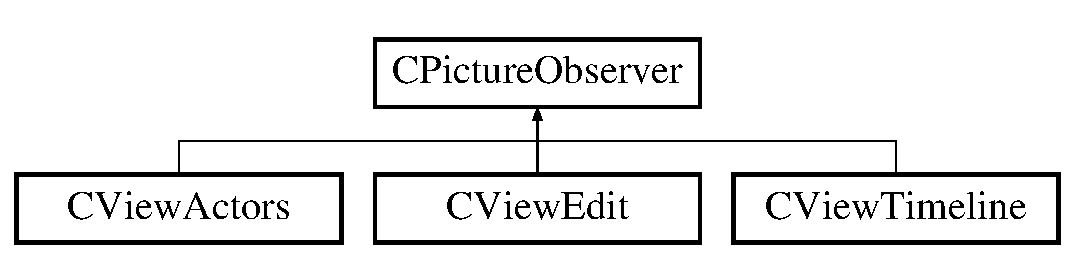
\includegraphics[height=2.000000cm]{class_c_picture_observer}
\end{center}
\end{figure}
\subsection*{Public Member Functions}
\begin{DoxyCompactItemize}
\item 
\hypertarget{class_c_picture_observer_a86036f6ad66ae4bad3f204f61d234f46}{virtual \hyperlink{class_c_picture_observer_a86036f6ad66ae4bad3f204f61d234f46}{$\sim$\+C\+Picture\+Observer} ()}\label{class_c_picture_observer_a86036f6ad66ae4bad3f204f61d234f46}

\begin{DoxyCompactList}\small\item\em Destructor. \end{DoxyCompactList}\item 
\hypertarget{class_c_picture_observer_a7c0cae97a7c165b98a00aeb2892cd6e7}{\hyperlink{class_c_picture_observer_a7c0cae97a7c165b98a00aeb2892cd6e7}{C\+Picture\+Observer} (const \hyperlink{class_c_picture_observer}{C\+Picture\+Observer} \&)=delete}\label{class_c_picture_observer_a7c0cae97a7c165b98a00aeb2892cd6e7}

\begin{DoxyCompactList}\small\item\em Copy Constructor (Disabled) \end{DoxyCompactList}\item 
\hypertarget{class_c_picture_observer_a200c66fe9ab13e18e9559033165b1895}{\hyperlink{class_c_picture_observer}{C\+Picture\+Observer} \& \hyperlink{class_c_picture_observer_a200c66fe9ab13e18e9559033165b1895}{operator=} (const \hyperlink{class_c_picture_observer}{C\+Picture\+Observer} \&)=delete}\label{class_c_picture_observer_a200c66fe9ab13e18e9559033165b1895}

\begin{DoxyCompactList}\small\item\em Assignment Operator (Disabled) \end{DoxyCompactList}\item 
\hypertarget{class_c_picture_observer_a0dce27216a8cb8a2490f0efc83a5994a}{virtual void \hyperlink{class_c_picture_observer_a0dce27216a8cb8a2490f0efc83a5994a}{Update\+Observer} ()=0}\label{class_c_picture_observer_a0dce27216a8cb8a2490f0efc83a5994a}

\begin{DoxyCompactList}\small\item\em This function is called to update any observers. \end{DoxyCompactList}\item 
void \hyperlink{class_c_picture_observer_a8f4bd1a0d4e3b14b511d572a6dadeb7e}{Set\+Picture} (std\+::shared\+\_\+ptr$<$ \hyperlink{class_c_picture}{C\+Picture} $>$ picture)
\begin{DoxyCompactList}\small\item\em Set the picture for this observer. \end{DoxyCompactList}\item 
std\+::shared\+\_\+ptr$<$ \hyperlink{class_c_picture}{C\+Picture} $>$ \hyperlink{class_c_picture_observer_ab7613c4badd101ace6a992b2eaaea153}{Get\+Picture} ()
\begin{DoxyCompactList}\small\item\em Get the picture this observer is associated with. \end{DoxyCompactList}\end{DoxyCompactItemize}


\subsection{Detailed Description}
Observer base class for a picture. 

This class implements the base class functionality for an observer in the observer pattern. 

\subsection{Member Function Documentation}
\hypertarget{class_c_picture_observer_ab7613c4badd101ace6a992b2eaaea153}{\index{C\+Picture\+Observer@{C\+Picture\+Observer}!Get\+Picture@{Get\+Picture}}
\index{Get\+Picture@{Get\+Picture}!C\+Picture\+Observer@{C\+Picture\+Observer}}
\subsubsection[{Get\+Picture}]{\setlength{\rightskip}{0pt plus 5cm}std\+::shared\+\_\+ptr$<${\bf C\+Picture}$>$ C\+Picture\+Observer\+::\+Get\+Picture (
\begin{DoxyParamCaption}
{}
\end{DoxyParamCaption}
)\hspace{0.3cm}{\ttfamily [inline]}}}\label{class_c_picture_observer_ab7613c4badd101ace6a992b2eaaea153}


Get the picture this observer is associated with. 

\begin{DoxyReturn}{Returns}
\hyperlink{class_c_picture}{C\+Picture} object 
\end{DoxyReturn}
\hypertarget{class_c_picture_observer_a8f4bd1a0d4e3b14b511d572a6dadeb7e}{\index{C\+Picture\+Observer@{C\+Picture\+Observer}!Set\+Picture@{Set\+Picture}}
\index{Set\+Picture@{Set\+Picture}!C\+Picture\+Observer@{C\+Picture\+Observer}}
\subsubsection[{Set\+Picture}]{\setlength{\rightskip}{0pt plus 5cm}void C\+Picture\+Observer\+::\+Set\+Picture (
\begin{DoxyParamCaption}
\item[{std\+::shared\+\_\+ptr$<$ {\bf C\+Picture} $>$}]{picture}
\end{DoxyParamCaption}
)}}\label{class_c_picture_observer_a8f4bd1a0d4e3b14b511d572a6dadeb7e}


Set the picture for this observer. 


\begin{DoxyParams}{Parameters}
{\em picture} & The picture to set \\
\hline
\end{DoxyParams}


The documentation for this class was generated from the following files\+:\begin{DoxyCompactItemize}
\item 
\hyperlink{_picture_observer_8h}{Picture\+Observer.\+h}\item 
\hyperlink{_picture_observer_8cpp}{Picture\+Observer.\+cpp}\end{DoxyCompactItemize}

\hypertarget{class_c_poly_drawable}{\section{C\+Poly\+Drawable Class Reference}
\label{class_c_poly_drawable}\index{C\+Poly\+Drawable@{C\+Poly\+Drawable}}
}


A drawable based on polygon images.  




{\ttfamily \#include $<$Poly\+Drawable.\+h$>$}

Inheritance diagram for C\+Poly\+Drawable\+:\begin{figure}[H]
\begin{center}
\leavevmode
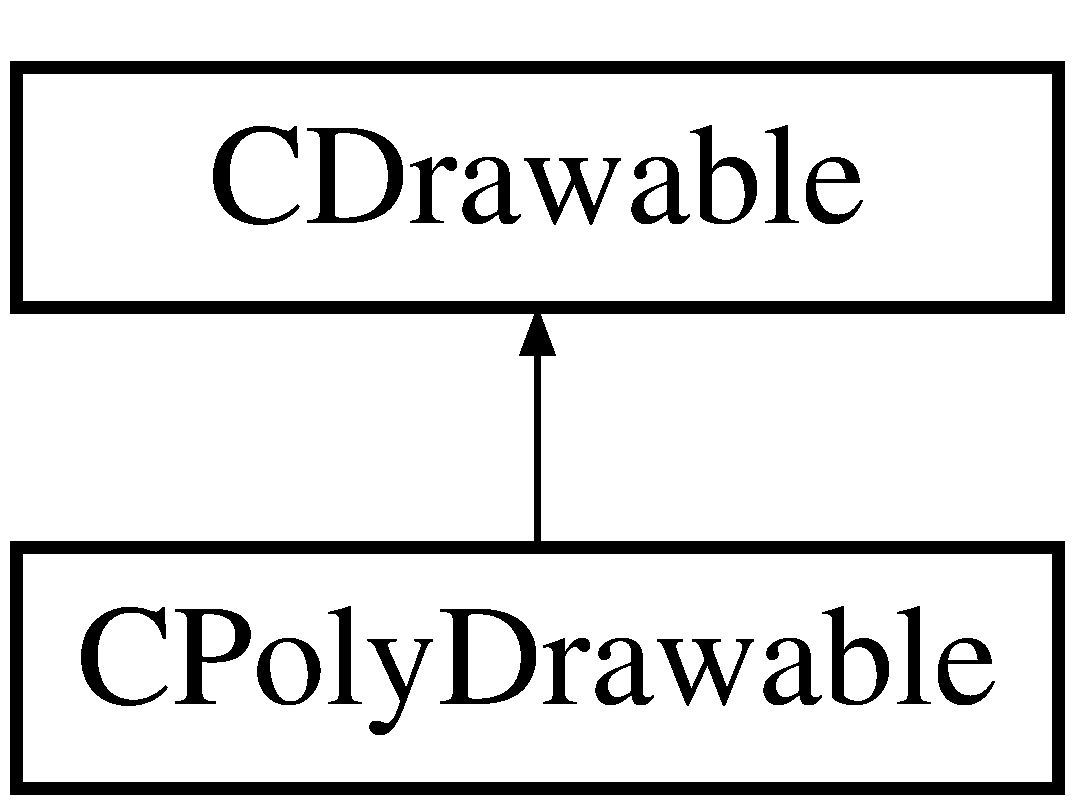
\includegraphics[height=2.000000cm]{class_c_poly_drawable}
\end{center}
\end{figure}
\subsection*{Public Member Functions}
\begin{DoxyCompactItemize}
\item 
\hyperlink{class_c_poly_drawable_a0afc2421a1a15fa7065423ccbe6d6ecc}{C\+Poly\+Drawable} (const std\+::wstring \&name)
\begin{DoxyCompactList}\small\item\em Constructor for a polygon object. \end{DoxyCompactList}\item 
\hypertarget{class_c_poly_drawable_afc766fdf8f37312434063b3b615f410b}{virtual \hyperlink{class_c_poly_drawable_afc766fdf8f37312434063b3b615f410b}{$\sim$\+C\+Poly\+Drawable} ()}\label{class_c_poly_drawable_afc766fdf8f37312434063b3b615f410b}

\begin{DoxyCompactList}\small\item\em Destructor. \end{DoxyCompactList}\item 
\hypertarget{class_c_poly_drawable_ae4265afa898200aa70a943cdea3f8123}{\hyperlink{class_c_poly_drawable_ae4265afa898200aa70a943cdea3f8123}{C\+Poly\+Drawable} ()=delete}\label{class_c_poly_drawable_ae4265afa898200aa70a943cdea3f8123}

\begin{DoxyCompactList}\small\item\em Default constructor disabled. \end{DoxyCompactList}\item 
\hypertarget{class_c_poly_drawable_abfdd10484ab2cb6ea99c01849cad4082}{\hyperlink{class_c_poly_drawable_abfdd10484ab2cb6ea99c01849cad4082}{C\+Poly\+Drawable} (const \hyperlink{class_c_poly_drawable}{C\+Poly\+Drawable} \&)=delete}\label{class_c_poly_drawable_abfdd10484ab2cb6ea99c01849cad4082}

\begin{DoxyCompactList}\small\item\em Copy constructor disabled. \end{DoxyCompactList}\item 
\hypertarget{class_c_poly_drawable_a86a6c65081b7feb556e5563b36a6ac8a}{void \hyperlink{class_c_poly_drawable_a86a6c65081b7feb556e5563b36a6ac8a}{operator=} (const \hyperlink{class_c_poly_drawable}{C\+Poly\+Drawable} \&)=delete}\label{class_c_poly_drawable_a86a6c65081b7feb556e5563b36a6ac8a}

\begin{DoxyCompactList}\small\item\em Assignment operator disabled. \end{DoxyCompactList}\item 
virtual void \hyperlink{class_c_poly_drawable_a701f45c8fabdec3de96b3048aa3a0190}{Draw} (Gdiplus\+::\+Graphics $\ast$graphics) override
\begin{DoxyCompactList}\small\item\em Draw our polygon. \end{DoxyCompactList}\item 
virtual bool \hyperlink{class_c_poly_drawable_a4db3493e3bba3c4c51608a75d48f50e2}{Hit\+Test} (Gdiplus\+::\+Point pos) override
\begin{DoxyCompactList}\small\item\em Test to see if we hit this object with a mouse click. \end{DoxyCompactList}\item 
void \hyperlink{class_c_poly_drawable_a500a475002f4be3cfe6ed865aea0a827}{Add\+Point} (Gdiplus\+::\+Point point)
\begin{DoxyCompactList}\small\item\em Add a point to the polygon. \end{DoxyCompactList}\item 
void \hyperlink{class_c_poly_drawable_a5d57281021db882ae059152f6f304aa0}{Set\+Color} (Gdiplus\+::\+Color color)
\begin{DoxyCompactList}\small\item\em Set the color for the polygon. \end{DoxyCompactList}\item 
Gdiplus\+::\+Color \hyperlink{class_c_poly_drawable_a441ecfc08876545cfe6f49cc81365328}{Get\+Color} () const 
\begin{DoxyCompactList}\small\item\em Get the drawable color. \end{DoxyCompactList}\end{DoxyCompactItemize}
\subsection*{Additional Inherited Members}


\subsection{Detailed Description}
A drawable based on polygon images. 

This class has a list of points and draws a polygon drawable based on those points. 

\subsection{Constructor \& Destructor Documentation}
\hypertarget{class_c_poly_drawable_a0afc2421a1a15fa7065423ccbe6d6ecc}{\index{C\+Poly\+Drawable@{C\+Poly\+Drawable}!C\+Poly\+Drawable@{C\+Poly\+Drawable}}
\index{C\+Poly\+Drawable@{C\+Poly\+Drawable}!C\+Poly\+Drawable@{C\+Poly\+Drawable}}
\subsubsection[{C\+Poly\+Drawable}]{\setlength{\rightskip}{0pt plus 5cm}C\+Poly\+Drawable\+::\+C\+Poly\+Drawable (
\begin{DoxyParamCaption}
\item[{const std\+::wstring \&}]{name}
\end{DoxyParamCaption}
)}}\label{class_c_poly_drawable_a0afc2421a1a15fa7065423ccbe6d6ecc}


Constructor for a polygon object. 


\begin{DoxyParams}{Parameters}
{\em name} & The drawable name \\
\hline
\end{DoxyParams}


\subsection{Member Function Documentation}
\hypertarget{class_c_poly_drawable_a500a475002f4be3cfe6ed865aea0a827}{\index{C\+Poly\+Drawable@{C\+Poly\+Drawable}!Add\+Point@{Add\+Point}}
\index{Add\+Point@{Add\+Point}!C\+Poly\+Drawable@{C\+Poly\+Drawable}}
\subsubsection[{Add\+Point}]{\setlength{\rightskip}{0pt plus 5cm}void C\+Poly\+Drawable\+::\+Add\+Point (
\begin{DoxyParamCaption}
\item[{Gdiplus\+::\+Point}]{point}
\end{DoxyParamCaption}
)}}\label{class_c_poly_drawable_a500a475002f4be3cfe6ed865aea0a827}


Add a point to the polygon. 


\begin{DoxyParams}{Parameters}
{\em point} & Point to add \\
\hline
\end{DoxyParams}
\hypertarget{class_c_poly_drawable_a701f45c8fabdec3de96b3048aa3a0190}{\index{C\+Poly\+Drawable@{C\+Poly\+Drawable}!Draw@{Draw}}
\index{Draw@{Draw}!C\+Poly\+Drawable@{C\+Poly\+Drawable}}
\subsubsection[{Draw}]{\setlength{\rightskip}{0pt plus 5cm}void C\+Poly\+Drawable\+::\+Draw (
\begin{DoxyParamCaption}
\item[{Gdiplus\+::\+Graphics $\ast$}]{graphics}
\end{DoxyParamCaption}
)\hspace{0.3cm}{\ttfamily [override]}, {\ttfamily [virtual]}}}\label{class_c_poly_drawable_a701f45c8fabdec3de96b3048aa3a0190}


Draw our polygon. 


\begin{DoxyParams}{Parameters}
{\em graphics} & The graphics context to draw on \\
\hline
\end{DoxyParams}


Implements \hyperlink{class_c_drawable_a9b6a9920a75d88d9ae321997495eaec7}{C\+Drawable}.

\hypertarget{class_c_poly_drawable_a441ecfc08876545cfe6f49cc81365328}{\index{C\+Poly\+Drawable@{C\+Poly\+Drawable}!Get\+Color@{Get\+Color}}
\index{Get\+Color@{Get\+Color}!C\+Poly\+Drawable@{C\+Poly\+Drawable}}
\subsubsection[{Get\+Color}]{\setlength{\rightskip}{0pt plus 5cm}Gdiplus\+::\+Color C\+Poly\+Drawable\+::\+Get\+Color (
\begin{DoxyParamCaption}
{}
\end{DoxyParamCaption}
) const\hspace{0.3cm}{\ttfamily [inline]}}}\label{class_c_poly_drawable_a441ecfc08876545cfe6f49cc81365328}


Get the drawable color. 

\begin{DoxyReturn}{Returns}
Color 
\end{DoxyReturn}
\hypertarget{class_c_poly_drawable_a4db3493e3bba3c4c51608a75d48f50e2}{\index{C\+Poly\+Drawable@{C\+Poly\+Drawable}!Hit\+Test@{Hit\+Test}}
\index{Hit\+Test@{Hit\+Test}!C\+Poly\+Drawable@{C\+Poly\+Drawable}}
\subsubsection[{Hit\+Test}]{\setlength{\rightskip}{0pt plus 5cm}bool C\+Poly\+Drawable\+::\+Hit\+Test (
\begin{DoxyParamCaption}
\item[{Gdiplus\+::\+Point}]{pos}
\end{DoxyParamCaption}
)\hspace{0.3cm}{\ttfamily [override]}, {\ttfamily [virtual]}}}\label{class_c_poly_drawable_a4db3493e3bba3c4c51608a75d48f50e2}


Test to see if we hit this object with a mouse click. 


\begin{DoxyParams}{Parameters}
{\em pos} & Click position \\
\hline
\end{DoxyParams}
\begin{DoxyReturn}{Returns}
true it hit 
\end{DoxyReturn}


Implements \hyperlink{class_c_drawable_a43490aec87b1209bbf7441e3855f0874}{C\+Drawable}.

\hypertarget{class_c_poly_drawable_a5d57281021db882ae059152f6f304aa0}{\index{C\+Poly\+Drawable@{C\+Poly\+Drawable}!Set\+Color@{Set\+Color}}
\index{Set\+Color@{Set\+Color}!C\+Poly\+Drawable@{C\+Poly\+Drawable}}
\subsubsection[{Set\+Color}]{\setlength{\rightskip}{0pt plus 5cm}void C\+Poly\+Drawable\+::\+Set\+Color (
\begin{DoxyParamCaption}
\item[{Gdiplus\+::\+Color}]{color}
\end{DoxyParamCaption}
)\hspace{0.3cm}{\ttfamily [inline]}}}\label{class_c_poly_drawable_a5d57281021db882ae059152f6f304aa0}


Set the color for the polygon. 


\begin{DoxyParams}{Parameters}
{\em color} & New color to set \\
\hline
\end{DoxyParams}


The documentation for this class was generated from the following files\+:\begin{DoxyCompactItemize}
\item 
\hyperlink{_poly_drawable_8h}{Poly\+Drawable.\+h}\item 
\hyperlink{_poly_drawable_8cpp}{Poly\+Drawable.\+cpp}\end{DoxyCompactItemize}

\hypertarget{class_c_rotated_bitmap}{\section{C\+Rotated\+Bitmap Class Reference}
\label{class_c_rotated_bitmap}\index{C\+Rotated\+Bitmap@{C\+Rotated\+Bitmap}}
}


Base class for a rotated bitmap.  




{\ttfamily \#include $<$Rotated\+Bitmap.\+h$>$}

Inheritance diagram for C\+Rotated\+Bitmap\+:\begin{figure}[H]
\begin{center}
\leavevmode
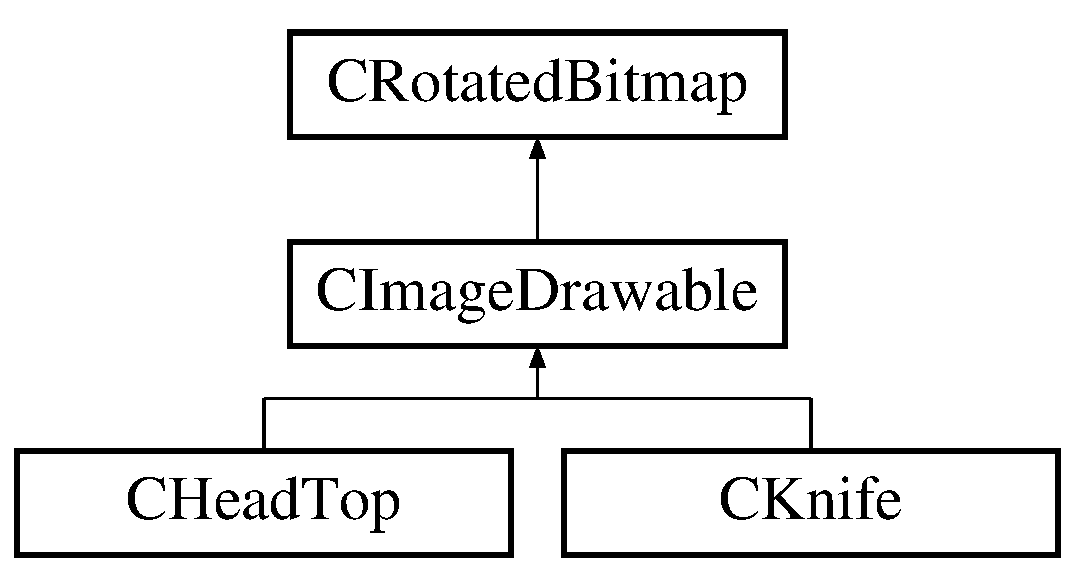
\includegraphics[height=3.000000cm]{class_c_rotated_bitmap}
\end{center}
\end{figure}
\subsection*{Public Member Functions}
\begin{DoxyCompactItemize}
\item 
\hypertarget{class_c_rotated_bitmap_a365819034778a6afbb1b10d4901ace2f}{\hyperlink{class_c_rotated_bitmap_a365819034778a6afbb1b10d4901ace2f}{C\+Rotated\+Bitmap} ()}\label{class_c_rotated_bitmap_a365819034778a6afbb1b10d4901ace2f}

\begin{DoxyCompactList}\small\item\em Constructor. \end{DoxyCompactList}\item 
\hypertarget{class_c_rotated_bitmap_ac8e1965b53e52ed4e9f136922323a995}{virtual \hyperlink{class_c_rotated_bitmap_ac8e1965b53e52ed4e9f136922323a995}{$\sim$\+C\+Rotated\+Bitmap} ()}\label{class_c_rotated_bitmap_ac8e1965b53e52ed4e9f136922323a995}

\begin{DoxyCompactList}\small\item\em Destructor. \end{DoxyCompactList}\item 
\hypertarget{class_c_rotated_bitmap_a1d8ebcd9419be8f843424bbf358bf97b}{\hyperlink{class_c_rotated_bitmap_a1d8ebcd9419be8f843424bbf358bf97b}{C\+Rotated\+Bitmap} (const \hyperlink{class_c_rotated_bitmap}{C\+Rotated\+Bitmap} \&)=delete}\label{class_c_rotated_bitmap_a1d8ebcd9419be8f843424bbf358bf97b}

\begin{DoxyCompactList}\small\item\em Copy constructor disabled. \end{DoxyCompactList}\item 
\hypertarget{class_c_rotated_bitmap_acd754404ab66f7f2f8336eaa5d9391cb}{void \hyperlink{class_c_rotated_bitmap_acd754404ab66f7f2f8336eaa5d9391cb}{operator=} (const \hyperlink{class_c_rotated_bitmap}{C\+Rotated\+Bitmap} \&)=delete}\label{class_c_rotated_bitmap_acd754404ab66f7f2f8336eaa5d9391cb}

\begin{DoxyCompactList}\small\item\em Assignment operator disabled. \end{DoxyCompactList}\item 
void \hyperlink{class_c_rotated_bitmap_ab4bd32142fb989ebd61cf6f948a9b27f}{Load\+Image} (const std\+::wstring \&filename)
\begin{DoxyCompactList}\small\item\em Load the image from a file. \end{DoxyCompactList}\item 
void \hyperlink{class_c_rotated_bitmap_a335b9038c2df31f3517486d2e36d1928}{Draw\+Image} (Gdiplus\+::\+Graphics $\ast$graphics, Gdiplus\+::\+Point position, double angle)
\begin{DoxyCompactList}\small\item\em Draw the bitmap. \end{DoxyCompactList}\item 
void \hyperlink{class_c_rotated_bitmap_a1c1e4efb36d0d3512a3ffd355817d409}{Set\+Center} (Gdiplus\+::\+Point center)
\begin{DoxyCompactList}\small\item\em Set the center to rotate around. \end{DoxyCompactList}\item 
Gdiplus\+::\+Point \hyperlink{class_c_rotated_bitmap_ac721fb576d19da95a5640d729260fbe7}{Get\+Center} () const 
\begin{DoxyCompactList}\small\item\em Get the center to rotate around. \end{DoxyCompactList}\item 
bool \hyperlink{class_c_rotated_bitmap_ae8a14cdbc38ca7a7b15a665de89ab142}{Is\+Loaded} () const 
\begin{DoxyCompactList}\small\item\em Is this bitmap loaded for use? \end{DoxyCompactList}\end{DoxyCompactItemize}
\subsection*{Protected Attributes}
\begin{DoxyCompactItemize}
\item 
\hypertarget{class_c_rotated_bitmap_aacdd9cba61ed0a8a5b90ee0a40bc18df}{std\+::unique\+\_\+ptr$<$ Gdiplus\+::\+Bitmap $>$ \hyperlink{class_c_rotated_bitmap_aacdd9cba61ed0a8a5b90ee0a40bc18df}{m\+Image}}\label{class_c_rotated_bitmap_aacdd9cba61ed0a8a5b90ee0a40bc18df}

\begin{DoxyCompactList}\small\item\em The image for this drawable. \end{DoxyCompactList}\item 
\hypertarget{class_c_rotated_bitmap_a67c587b5b5d6dfb609708a3c62f37a0d}{Gdiplus\+::\+Point \hyperlink{class_c_rotated_bitmap_a67c587b5b5d6dfb609708a3c62f37a0d}{m\+Center} = Gdiplus\+::\+Point(0, 0)}\label{class_c_rotated_bitmap_a67c587b5b5d6dfb609708a3c62f37a0d}

\begin{DoxyCompactList}\small\item\em The center of the image. \end{DoxyCompactList}\item 
\hypertarget{class_c_rotated_bitmap_a99f6dbd45bf8cb36b1eaa101520789bf}{bool \hyperlink{class_c_rotated_bitmap_a99f6dbd45bf8cb36b1eaa101520789bf}{m\+Loaded} = false}\label{class_c_rotated_bitmap_a99f6dbd45bf8cb36b1eaa101520789bf}

\begin{DoxyCompactList}\small\item\em Has an image been loaded? \end{DoxyCompactList}\end{DoxyCompactItemize}


\subsection{Detailed Description}
Base class for a rotated bitmap. 

\subsection{Member Function Documentation}
\hypertarget{class_c_rotated_bitmap_a335b9038c2df31f3517486d2e36d1928}{\index{C\+Rotated\+Bitmap@{C\+Rotated\+Bitmap}!Draw\+Image@{Draw\+Image}}
\index{Draw\+Image@{Draw\+Image}!C\+Rotated\+Bitmap@{C\+Rotated\+Bitmap}}
\subsubsection[{Draw\+Image}]{\setlength{\rightskip}{0pt plus 5cm}void C\+Rotated\+Bitmap\+::\+Draw\+Image (
\begin{DoxyParamCaption}
\item[{Gdiplus\+::\+Graphics $\ast$}]{graphics, }
\item[{Gdiplus\+::\+Point}]{position, }
\item[{double}]{angle}
\end{DoxyParamCaption}
)}}\label{class_c_rotated_bitmap_a335b9038c2df31f3517486d2e36d1928}


Draw the bitmap. 


\begin{DoxyParams}{Parameters}
{\em graphics} & The graphics context to draw on \\
\hline
{\em position} & The position to draw at \\
\hline
{\em angle} & The rotation angle \\
\hline
\end{DoxyParams}
\hypertarget{class_c_rotated_bitmap_ac721fb576d19da95a5640d729260fbe7}{\index{C\+Rotated\+Bitmap@{C\+Rotated\+Bitmap}!Get\+Center@{Get\+Center}}
\index{Get\+Center@{Get\+Center}!C\+Rotated\+Bitmap@{C\+Rotated\+Bitmap}}
\subsubsection[{Get\+Center}]{\setlength{\rightskip}{0pt plus 5cm}Gdiplus\+::\+Point C\+Rotated\+Bitmap\+::\+Get\+Center (
\begin{DoxyParamCaption}
{}
\end{DoxyParamCaption}
) const\hspace{0.3cm}{\ttfamily [inline]}}}\label{class_c_rotated_bitmap_ac721fb576d19da95a5640d729260fbe7}


Get the center to rotate around. 

\begin{DoxyReturn}{Returns}
Center 
\end{DoxyReturn}
\hypertarget{class_c_rotated_bitmap_ae8a14cdbc38ca7a7b15a665de89ab142}{\index{C\+Rotated\+Bitmap@{C\+Rotated\+Bitmap}!Is\+Loaded@{Is\+Loaded}}
\index{Is\+Loaded@{Is\+Loaded}!C\+Rotated\+Bitmap@{C\+Rotated\+Bitmap}}
\subsubsection[{Is\+Loaded}]{\setlength{\rightskip}{0pt plus 5cm}bool C\+Rotated\+Bitmap\+::\+Is\+Loaded (
\begin{DoxyParamCaption}
{}
\end{DoxyParamCaption}
) const\hspace{0.3cm}{\ttfamily [inline]}}}\label{class_c_rotated_bitmap_ae8a14cdbc38ca7a7b15a665de89ab142}


Is this bitmap loaded for use? 

\begin{DoxyReturn}{Returns}
true if loaded 
\end{DoxyReturn}
\hypertarget{class_c_rotated_bitmap_ab4bd32142fb989ebd61cf6f948a9b27f}{\index{C\+Rotated\+Bitmap@{C\+Rotated\+Bitmap}!Load\+Image@{Load\+Image}}
\index{Load\+Image@{Load\+Image}!C\+Rotated\+Bitmap@{C\+Rotated\+Bitmap}}
\subsubsection[{Load\+Image}]{\setlength{\rightskip}{0pt plus 5cm}void C\+Rotated\+Bitmap\+::\+Load\+Image (
\begin{DoxyParamCaption}
\item[{const std\+::wstring \&}]{filename}
\end{DoxyParamCaption}
)}}\label{class_c_rotated_bitmap_ab4bd32142fb989ebd61cf6f948a9b27f}


Load the image from a file. 


\begin{DoxyParams}{Parameters}
{\em filename} & File to load \\
\hline
\end{DoxyParams}
\hypertarget{class_c_rotated_bitmap_a1c1e4efb36d0d3512a3ffd355817d409}{\index{C\+Rotated\+Bitmap@{C\+Rotated\+Bitmap}!Set\+Center@{Set\+Center}}
\index{Set\+Center@{Set\+Center}!C\+Rotated\+Bitmap@{C\+Rotated\+Bitmap}}
\subsubsection[{Set\+Center}]{\setlength{\rightskip}{0pt plus 5cm}void C\+Rotated\+Bitmap\+::\+Set\+Center (
\begin{DoxyParamCaption}
\item[{Gdiplus\+::\+Point}]{center}
\end{DoxyParamCaption}
)\hspace{0.3cm}{\ttfamily [inline]}}}\label{class_c_rotated_bitmap_a1c1e4efb36d0d3512a3ffd355817d409}


Set the center to rotate around. 


\begin{DoxyParams}{Parameters}
{\em center} & New center \\
\hline
\end{DoxyParams}


The documentation for this class was generated from the following files\+:\begin{DoxyCompactItemize}
\item 
\hyperlink{_rotated_bitmap_8h}{Rotated\+Bitmap.\+h}\item 
\hyperlink{_rotated_bitmap_8cpp}{Rotated\+Bitmap.\+cpp}\end{DoxyCompactItemize}

\hypertarget{class_c_snowflake}{\section{C\+Snowflake Class Reference}
\label{class_c_snowflake}\index{C\+Snowflake@{C\+Snowflake}}
}


The snow flake class to implement snow.  




{\ttfamily \#include $<$Snowflake.\+h$>$}

\subsection*{Public Member Functions}
\begin{DoxyCompactItemize}
\item 
\hypertarget{class_c_snowflake_a839815275ab5ca42c8545e39a04b2f75}{\hyperlink{class_c_snowflake_a839815275ab5ca42c8545e39a04b2f75}{C\+Snowflake} ()}\label{class_c_snowflake_a839815275ab5ca42c8545e39a04b2f75}

\begin{DoxyCompactList}\small\item\em Constructor. \end{DoxyCompactList}\item 
\hypertarget{class_c_snowflake_a0e8738c0d7fc9c2ab354e93532f62df2}{\hyperlink{class_c_snowflake_a0e8738c0d7fc9c2ab354e93532f62df2}{$\sim$\+C\+Snowflake} ()}\label{class_c_snowflake_a0e8738c0d7fc9c2ab354e93532f62df2}

\begin{DoxyCompactList}\small\item\em Destructor. \end{DoxyCompactList}\item 
void \hyperlink{class_c_snowflake_a1002ccff7dc55143e7e9879f7f6ab8fb}{Draw} (Gdiplus\+::\+Graphics $\ast$graphics, Gdiplus\+::\+Solid\+Brush $\ast$brush)
\begin{DoxyCompactList}\small\item\em The function to draw the snow flakes. \end{DoxyCompactList}\item 
void \hyperlink{class_c_snowflake_a4ff5173791cdab56885c9ae1dced9d05}{Update} (double elapsed)
\begin{DoxyCompactList}\small\item\em The update function to redraw the snowflake. \end{DoxyCompactList}\item 
std\+::shared\+\_\+ptr$<$ \hyperlink{class_c_snowflake}{C\+Snowflake} $>$ \hyperlink{class_c_snowflake_ae228ed6b4121315e019efc5ff7acd2e8}{Get\+Next} ()
\begin{DoxyCompactList}\small\item\em The getter function to get the pointer next. \end{DoxyCompactList}\item 
void \hyperlink{class_c_snowflake_a5a763ea12e70d4e4fb82571636f761ef}{Set\+Next} (std\+::shared\+\_\+ptr$<$ \hyperlink{class_c_snowflake}{C\+Snowflake} $>$ n)
\begin{DoxyCompactList}\small\item\em setter function to set the pointer next \end{DoxyCompactList}\item 
void \hyperlink{class_c_snowflake_a4a5c3acf9fe94454a3409ace089356ea}{Set\+Position} (double x, double y)
\begin{DoxyCompactList}\small\item\em setter function to set the position \end{DoxyCompactList}\item 
int \hyperlink{class_c_snowflake_a785bd07f9b7341606e94204e6be7af67}{Get\+Position\+X} ()
\begin{DoxyCompactList}\small\item\em The getter function to get the x position. \end{DoxyCompactList}\item 
int \hyperlink{class_c_snowflake_a047611d7e82786fec3d329f4579ef823}{Get\+Position\+Y} ()
\begin{DoxyCompactList}\small\item\em The getter function to get the y position. \end{DoxyCompactList}\end{DoxyCompactItemize}


\subsection{Detailed Description}
The snow flake class to implement snow. 

\subsection{Member Function Documentation}
\hypertarget{class_c_snowflake_a1002ccff7dc55143e7e9879f7f6ab8fb}{\index{C\+Snowflake@{C\+Snowflake}!Draw@{Draw}}
\index{Draw@{Draw}!C\+Snowflake@{C\+Snowflake}}
\subsubsection[{Draw}]{\setlength{\rightskip}{0pt plus 5cm}void C\+Snowflake\+::\+Draw (
\begin{DoxyParamCaption}
\item[{Gdiplus\+::\+Graphics $\ast$}]{graphics, }
\item[{Gdiplus\+::\+Solid\+Brush $\ast$}]{brush}
\end{DoxyParamCaption}
)}}\label{class_c_snowflake_a1002ccff7dc55143e7e9879f7f6ab8fb}


The function to draw the snow flakes. 


\begin{DoxyParams}{Parameters}
{\em graphics} & The device context to draw on \\
\hline
{\em brush} & The corlor brush to dawn with \\
\hline
\end{DoxyParams}
\hypertarget{class_c_snowflake_ae228ed6b4121315e019efc5ff7acd2e8}{\index{C\+Snowflake@{C\+Snowflake}!Get\+Next@{Get\+Next}}
\index{Get\+Next@{Get\+Next}!C\+Snowflake@{C\+Snowflake}}
\subsubsection[{Get\+Next}]{\setlength{\rightskip}{0pt plus 5cm}std\+::shared\+\_\+ptr$<${\bf C\+Snowflake}$>$ C\+Snowflake\+::\+Get\+Next (
\begin{DoxyParamCaption}
{}
\end{DoxyParamCaption}
)\hspace{0.3cm}{\ttfamily [inline]}}}\label{class_c_snowflake_ae228ed6b4121315e019efc5ff7acd2e8}


The getter function to get the pointer next. 

\begin{DoxyReturn}{Returns}
The pointer to next 
\end{DoxyReturn}
\hypertarget{class_c_snowflake_a785bd07f9b7341606e94204e6be7af67}{\index{C\+Snowflake@{C\+Snowflake}!Get\+Position\+X@{Get\+Position\+X}}
\index{Get\+Position\+X@{Get\+Position\+X}!C\+Snowflake@{C\+Snowflake}}
\subsubsection[{Get\+Position\+X}]{\setlength{\rightskip}{0pt plus 5cm}int C\+Snowflake\+::\+Get\+Position\+X (
\begin{DoxyParamCaption}
{}
\end{DoxyParamCaption}
)\hspace{0.3cm}{\ttfamily [inline]}}}\label{class_c_snowflake_a785bd07f9b7341606e94204e6be7af67}


The getter function to get the x position. 

\begin{DoxyReturn}{Returns}
the x position 
\end{DoxyReturn}
\hypertarget{class_c_snowflake_a047611d7e82786fec3d329f4579ef823}{\index{C\+Snowflake@{C\+Snowflake}!Get\+Position\+Y@{Get\+Position\+Y}}
\index{Get\+Position\+Y@{Get\+Position\+Y}!C\+Snowflake@{C\+Snowflake}}
\subsubsection[{Get\+Position\+Y}]{\setlength{\rightskip}{0pt plus 5cm}int C\+Snowflake\+::\+Get\+Position\+Y (
\begin{DoxyParamCaption}
{}
\end{DoxyParamCaption}
)\hspace{0.3cm}{\ttfamily [inline]}}}\label{class_c_snowflake_a047611d7e82786fec3d329f4579ef823}


The getter function to get the y position. 

\begin{DoxyReturn}{Returns}
the y position 
\end{DoxyReturn}
\hypertarget{class_c_snowflake_a5a763ea12e70d4e4fb82571636f761ef}{\index{C\+Snowflake@{C\+Snowflake}!Set\+Next@{Set\+Next}}
\index{Set\+Next@{Set\+Next}!C\+Snowflake@{C\+Snowflake}}
\subsubsection[{Set\+Next}]{\setlength{\rightskip}{0pt plus 5cm}void C\+Snowflake\+::\+Set\+Next (
\begin{DoxyParamCaption}
\item[{std\+::shared\+\_\+ptr$<$ {\bf C\+Snowflake} $>$}]{n}
\end{DoxyParamCaption}
)\hspace{0.3cm}{\ttfamily [inline]}}}\label{class_c_snowflake_a5a763ea12e70d4e4fb82571636f761ef}


setter function to set the pointer next 


\begin{DoxyParams}{Parameters}
{\em n} & pointer to next \\
\hline
\end{DoxyParams}
\hypertarget{class_c_snowflake_a4a5c3acf9fe94454a3409ace089356ea}{\index{C\+Snowflake@{C\+Snowflake}!Set\+Position@{Set\+Position}}
\index{Set\+Position@{Set\+Position}!C\+Snowflake@{C\+Snowflake}}
\subsubsection[{Set\+Position}]{\setlength{\rightskip}{0pt plus 5cm}void C\+Snowflake\+::\+Set\+Position (
\begin{DoxyParamCaption}
\item[{double}]{x, }
\item[{double}]{y}
\end{DoxyParamCaption}
)\hspace{0.3cm}{\ttfamily [inline]}}}\label{class_c_snowflake_a4a5c3acf9fe94454a3409ace089356ea}


setter function to set the position 


\begin{DoxyParams}{Parameters}
{\em x,x} & coordinate; \\
\hline
{\em y,y} & coordinate \\
\hline
\end{DoxyParams}
\hypertarget{class_c_snowflake_a4ff5173791cdab56885c9ae1dced9d05}{\index{C\+Snowflake@{C\+Snowflake}!Update@{Update}}
\index{Update@{Update}!C\+Snowflake@{C\+Snowflake}}
\subsubsection[{Update}]{\setlength{\rightskip}{0pt plus 5cm}void C\+Snowflake\+::\+Update (
\begin{DoxyParamCaption}
\item[{double}]{elapsed}
\end{DoxyParamCaption}
)}}\label{class_c_snowflake_a4ff5173791cdab56885c9ae1dced9d05}


The update function to redraw the snowflake. 


\begin{DoxyParams}{Parameters}
{\em elapsed} & the time between each update \\
\hline
\end{DoxyParams}


The documentation for this class was generated from the following files\+:\begin{DoxyCompactItemize}
\item 
\hyperlink{_snowflake_8h}{Snowflake.\+h}\item 
\hyperlink{_snowflake_8cpp}{Snowflake.\+cpp}\end{DoxyCompactItemize}

\hypertarget{class_c_sparty_factory}{\section{C\+Sparty\+Factory Class Reference}
\label{class_c_sparty_factory}\index{C\+Sparty\+Factory@{C\+Sparty\+Factory}}
}


Factory that builds the Sparty actor.  




{\ttfamily \#include $<$Sparty\+Factory.\+h$>$}

Inheritance diagram for C\+Sparty\+Factory\+:\begin{figure}[H]
\begin{center}
\leavevmode
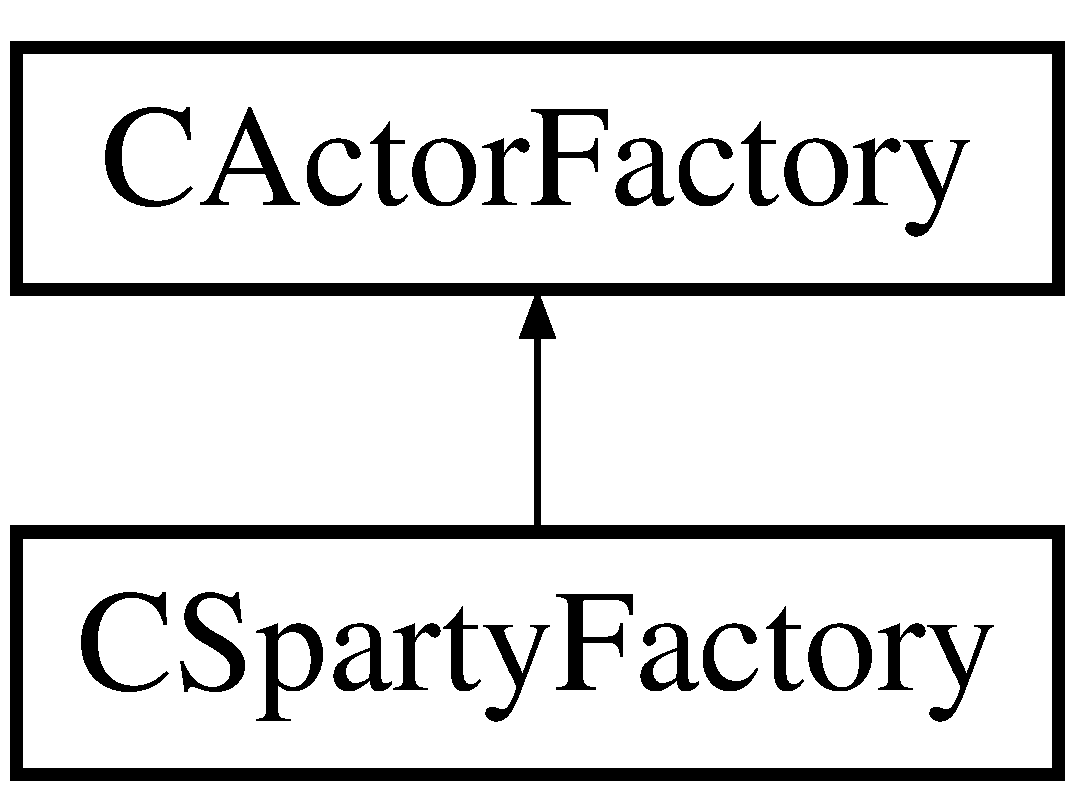
\includegraphics[height=2.000000cm]{class_c_sparty_factory}
\end{center}
\end{figure}
\subsection*{Public Member Functions}
\begin{DoxyCompactItemize}
\item 
\hypertarget{class_c_sparty_factory_a18c0a4465dbe6d11366aba4fe4ad9169}{\hyperlink{class_c_sparty_factory_a18c0a4465dbe6d11366aba4fe4ad9169}{C\+Sparty\+Factory} ()}\label{class_c_sparty_factory_a18c0a4465dbe6d11366aba4fe4ad9169}

\begin{DoxyCompactList}\small\item\em Constructor. \end{DoxyCompactList}\item 
\hypertarget{class_c_sparty_factory_a62cd08892f206bf5cb5a632e4e67e022}{virtual \hyperlink{class_c_sparty_factory_a62cd08892f206bf5cb5a632e4e67e022}{$\sim$\+C\+Sparty\+Factory} ()}\label{class_c_sparty_factory_a62cd08892f206bf5cb5a632e4e67e022}

\begin{DoxyCompactList}\small\item\em Destructor. \end{DoxyCompactList}\item 
std\+::shared\+\_\+ptr$<$ \hyperlink{class_c_actor}{C\+Actor} $>$ \hyperlink{class_c_sparty_factory_a171c122e80006b4adcc13a9e81faf3fc}{Create} ()
\begin{DoxyCompactList}\small\item\em This is a concrete factory method that creates our Harold actor. \end{DoxyCompactList}\end{DoxyCompactItemize}
\subsection*{Additional Inherited Members}


\subsection{Detailed Description}
Factory that builds the Sparty actor. 

\subsection{Member Function Documentation}
\hypertarget{class_c_sparty_factory_a171c122e80006b4adcc13a9e81faf3fc}{\index{C\+Sparty\+Factory@{C\+Sparty\+Factory}!Create@{Create}}
\index{Create@{Create}!C\+Sparty\+Factory@{C\+Sparty\+Factory}}
\subsubsection[{Create}]{\setlength{\rightskip}{0pt plus 5cm}std\+::shared\+\_\+ptr$<$ {\bf C\+Actor} $>$ C\+Sparty\+Factory\+::\+Create (
\begin{DoxyParamCaption}
{}
\end{DoxyParamCaption}
)\hspace{0.3cm}{\ttfamily [virtual]}}}\label{class_c_sparty_factory_a171c122e80006b4adcc13a9e81faf3fc}


This is a concrete factory method that creates our Harold actor. 

\begin{DoxyReturn}{Returns}
Pointer to an actor object. 
\end{DoxyReturn}


Implements \hyperlink{class_c_actor_factory_a1e751d97cc015ab2182b7683133e5a5d}{C\+Actor\+Factory}.



The documentation for this class was generated from the following files\+:\begin{DoxyCompactItemize}
\item 
\hyperlink{_sparty_factory_8h}{Sparty\+Factory.\+h}\item 
\hyperlink{_sparty_factory_8cpp}{Sparty\+Factory.\+cpp}\end{DoxyCompactItemize}

\hypertarget{class_c_text_bubble_drawable}{\section{C\+Text\+Bubble\+Drawable Class Reference}
\label{class_c_text_bubble_drawable}\index{C\+Text\+Bubble\+Drawable@{C\+Text\+Bubble\+Drawable}}
}


The text bubble class adpater.  




{\ttfamily \#include $<$Text\+Bubble\+Drawable.\+h$>$}

Inheritance diagram for C\+Text\+Bubble\+Drawable\+:\begin{figure}[H]
\begin{center}
\leavevmode
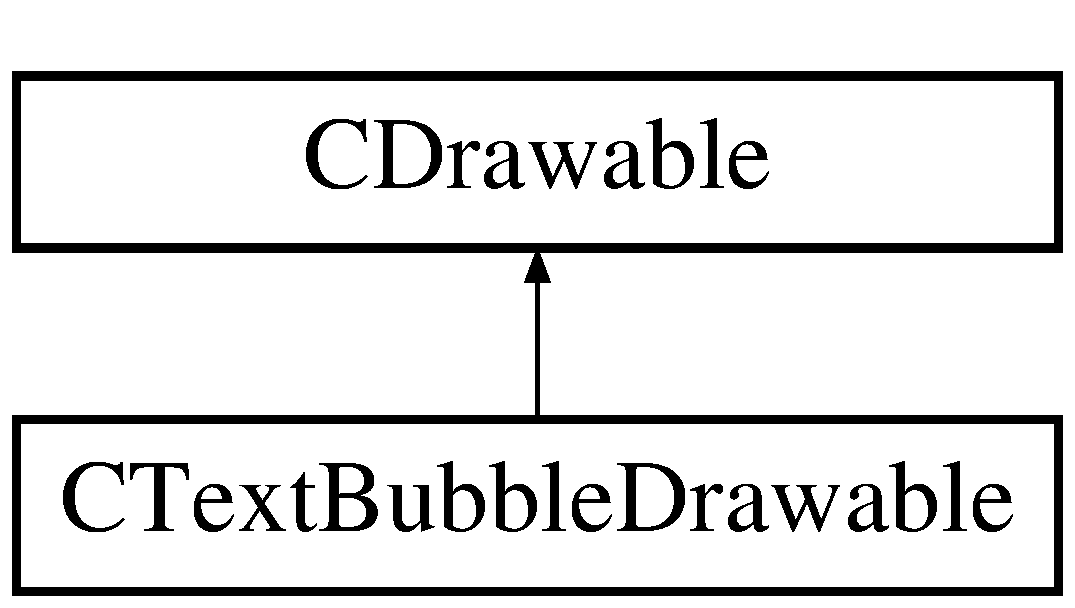
\includegraphics[height=2.000000cm]{class_c_text_bubble_drawable}
\end{center}
\end{figure}
\subsection*{Public Member Functions}
\begin{DoxyCompactItemize}
\item 
\hyperlink{class_c_text_bubble_drawable_a65188df7a034a6a4df50866b504abedb}{C\+Text\+Bubble\+Drawable} (const std\+::wstring \&name)
\begin{DoxyCompactList}\small\item\em Default constructor. \end{DoxyCompactList}\item 
\hypertarget{class_c_text_bubble_drawable_aa573f267e94aaf7f15940b30cae40141}{virtual \hyperlink{class_c_text_bubble_drawable_aa573f267e94aaf7f15940b30cae40141}{$\sim$\+C\+Text\+Bubble\+Drawable} ()}\label{class_c_text_bubble_drawable_aa573f267e94aaf7f15940b30cae40141}

\begin{DoxyCompactList}\small\item\em Destructor. \end{DoxyCompactList}\item 
\hypertarget{class_c_text_bubble_drawable_a4e7c9168364e4eb0c8765c2bbde378ef}{\hyperlink{class_c_text_bubble_drawable_a4e7c9168364e4eb0c8765c2bbde378ef}{C\+Text\+Bubble\+Drawable} ()=delete}\label{class_c_text_bubble_drawable_a4e7c9168364e4eb0c8765c2bbde378ef}

\begin{DoxyCompactList}\small\item\em Default constructor disabled. \end{DoxyCompactList}\item 
\hypertarget{class_c_text_bubble_drawable_a93a6ab5582897e65fafa41c8f9b8643c}{\hyperlink{class_c_text_bubble_drawable_a93a6ab5582897e65fafa41c8f9b8643c}{C\+Text\+Bubble\+Drawable} (const \hyperlink{class_c_text_bubble_drawable}{C\+Text\+Bubble\+Drawable} \&)=delete}\label{class_c_text_bubble_drawable_a93a6ab5582897e65fafa41c8f9b8643c}

\begin{DoxyCompactList}\small\item\em Copy constructor disabled. \end{DoxyCompactList}\item 
\hypertarget{class_c_text_bubble_drawable_aa1895ac0e75e9783e17634fc2d04447f}{void \hyperlink{class_c_text_bubble_drawable_aa1895ac0e75e9783e17634fc2d04447f}{operator=} (const \hyperlink{class_c_text_bubble_drawable}{C\+Text\+Bubble\+Drawable} \&)=delete}\label{class_c_text_bubble_drawable_aa1895ac0e75e9783e17634fc2d04447f}

\begin{DoxyCompactList}\small\item\em Assignment operator disabled. \end{DoxyCompactList}\item 
virtual void \hyperlink{class_c_text_bubble_drawable_ab06c08f5357aabd1275610baac806b59}{Draw} (Gdiplus\+::\+Graphics $\ast$graphics) override
\begin{DoxyCompactList}\small\item\em The Draw function to draw the text bubble. \end{DoxyCompactList}\item 
virtual bool \hyperlink{class_c_text_bubble_drawable_a85dd41fa9b6ce12989f529907030fd9a}{Hit\+Test} (Gdiplus\+::\+Point pos) override
\begin{DoxyCompactList}\small\item\em The Hittest function to check if the click is in the text bubble. \end{DoxyCompactList}\item 
\hypertarget{class_c_text_bubble_drawable_aa12d719c3c6e7d76edc3d0afdb5e9485}{virtual bool \hyperlink{class_c_text_bubble_drawable_aa12d719c3c6e7d76edc3d0afdb5e9485}{Is\+Movable} ()}\label{class_c_text_bubble_drawable_aa12d719c3c6e7d76edc3d0afdb5e9485}

\begin{DoxyCompactList}\small\item\em Check if the text bubble can be moved. \end{DoxyCompactList}\item 
virtual bool \hyperlink{class_c_text_bubble_drawable_a0ad09643af72c6fcd0182f38e8ce18da}{Is\+Text\+Bubble\+Drawable} () override
\begin{DoxyCompactList}\small\item\em Check the drawable is Text\+Bubble\+Drawable. \end{DoxyCompactList}\item 
\hypertarget{class_c_text_bubble_drawable_a61d871237611c8fc4f01f29bdee9dc58}{std\+::wstring \hyperlink{class_c_text_bubble_drawable_a61d871237611c8fc4f01f29bdee9dc58}{Get\+Text} ()}\label{class_c_text_bubble_drawable_a61d871237611c8fc4f01f29bdee9dc58}

\begin{DoxyCompactList}\small\item\em Get the text value from Text bubble class. \end{DoxyCompactList}\item 
\hypertarget{class_c_text_bubble_drawable_ae1b61142301c7ebb292917fb3988dd24}{bool \hyperlink{class_c_text_bubble_drawable_ae1b61142301c7ebb292917fb3988dd24}{Get\+Mirror} ()}\label{class_c_text_bubble_drawable_ae1b61142301c7ebb292917fb3988dd24}

\begin{DoxyCompactList}\small\item\em Get the mirror value from text bubbleclass. \end{DoxyCompactList}\item 
void \hyperlink{class_c_text_bubble_drawable_ac7d35d877413dfa7f633646a09e67ffe}{Set\+Text} (const std\+::wstring \&str)
\begin{DoxyCompactList}\small\item\em Set the text value in the text bubble. \end{DoxyCompactList}\item 
void \hyperlink{class_c_text_bubble_drawable_acb036cd5239ba203bb7cf55616a32b88}{Set\+Mirror} (const bool \&mirror)
\begin{DoxyCompactList}\small\item\em Get the mirror value in the text bubble. \end{DoxyCompactList}\item 
\hypertarget{class_c_text_bubble_drawable_a0df72f52a5df614eccdff89bf12cf905}{virtual C\+Text\+Bubble $\ast$ \hyperlink{class_c_text_bubble_drawable_a0df72f52a5df614eccdff89bf12cf905}{Get\+Text\+Bubble} () override}\label{class_c_text_bubble_drawable_a0df72f52a5df614eccdff89bf12cf905}

\begin{DoxyCompactList}\small\item\em Get the Text bubble this class adpated for. \end{DoxyCompactList}\item 
void \hyperlink{class_c_text_bubble_drawable_a6e154d1a283f3f0b85eb1f3d1480c21e}{Set\+Actor} (\hyperlink{class_c_actor}{C\+Actor} $\ast$actor)
\begin{DoxyCompactList}\small\item\em Set the actor. This is where we set the channel name. \end{DoxyCompactList}\item 
virtual void \hyperlink{class_c_text_bubble_drawable_adbf6b04696680906cc3cb32e7a0918b9}{Set\+Timeline} (\hyperlink{class_c_timeline}{C\+Timeline} $\ast$timeline) override
\begin{DoxyCompactList}\small\item\em Set the timeline. The tells the channel the timeline. \end{DoxyCompactList}\item 
\hypertarget{class_c_text_bubble_drawable_a360ce876ba0ccdb24a22bc356597e6d1}{virtual void \hyperlink{class_c_text_bubble_drawable_a360ce876ba0ccdb24a22bc356597e6d1}{Set\+Keyframe} () override}\label{class_c_text_bubble_drawable_a360ce876ba0ccdb24a22bc356597e6d1}

\begin{DoxyCompactList}\small\item\em Set the keyframe based on the current status. \end{DoxyCompactList}\item 
\hypertarget{class_c_text_bubble_drawable_ab6978a6de5ce63512f215d42f9f6e388}{virtual void \hyperlink{class_c_text_bubble_drawable_ab6978a6de5ce63512f215d42f9f6e388}{Get\+Keyframe} () override}\label{class_c_text_bubble_drawable_ab6978a6de5ce63512f215d42f9f6e388}

\begin{DoxyCompactList}\small\item\em Get the current channel from the animation system. \end{DoxyCompactList}\item 
\hyperlink{class_c_anim_channel_text}{C\+Anim\+Channel\+Text} $\ast$ \hyperlink{class_c_text_bubble_drawable_a62179412aeb297e04f996c69b3887e38}{Get\+Text\+Channel} ()
\begin{DoxyCompactList}\small\item\em The position animation channel. \end{DoxyCompactList}\end{DoxyCompactItemize}
\subsection*{Additional Inherited Members}


\subsection{Detailed Description}
The text bubble class adpater. 

\subsection{Constructor \& Destructor Documentation}
\hypertarget{class_c_text_bubble_drawable_a65188df7a034a6a4df50866b504abedb}{\index{C\+Text\+Bubble\+Drawable@{C\+Text\+Bubble\+Drawable}!C\+Text\+Bubble\+Drawable@{C\+Text\+Bubble\+Drawable}}
\index{C\+Text\+Bubble\+Drawable@{C\+Text\+Bubble\+Drawable}!C\+Text\+Bubble\+Drawable@{C\+Text\+Bubble\+Drawable}}
\subsubsection[{C\+Text\+Bubble\+Drawable}]{\setlength{\rightskip}{0pt plus 5cm}C\+Text\+Bubble\+Drawable\+::\+C\+Text\+Bubble\+Drawable (
\begin{DoxyParamCaption}
\item[{const std\+::wstring \&}]{name}
\end{DoxyParamCaption}
)}}\label{class_c_text_bubble_drawable_a65188df7a034a6a4df50866b504abedb}


Default constructor. 


\begin{DoxyParams}{Parameters}
{\em name} & of the bubble \\
\hline
\end{DoxyParams}


\subsection{Member Function Documentation}
\hypertarget{class_c_text_bubble_drawable_ab06c08f5357aabd1275610baac806b59}{\index{C\+Text\+Bubble\+Drawable@{C\+Text\+Bubble\+Drawable}!Draw@{Draw}}
\index{Draw@{Draw}!C\+Text\+Bubble\+Drawable@{C\+Text\+Bubble\+Drawable}}
\subsubsection[{Draw}]{\setlength{\rightskip}{0pt plus 5cm}void C\+Text\+Bubble\+Drawable\+::\+Draw (
\begin{DoxyParamCaption}
\item[{Gdiplus\+::\+Graphics $\ast$}]{graphics}
\end{DoxyParamCaption}
)\hspace{0.3cm}{\ttfamily [override]}, {\ttfamily [virtual]}}}\label{class_c_text_bubble_drawable_ab06c08f5357aabd1275610baac806b59}


The Draw function to draw the text bubble. 

The draw function to draw the text bubble.


\begin{DoxyParams}{Parameters}
{\em graphics} & \\
\hline
\end{DoxyParams}


Implements \hyperlink{class_c_drawable_a9b6a9920a75d88d9ae321997495eaec7}{C\+Drawable}.

\hypertarget{class_c_text_bubble_drawable_a62179412aeb297e04f996c69b3887e38}{\index{C\+Text\+Bubble\+Drawable@{C\+Text\+Bubble\+Drawable}!Get\+Text\+Channel@{Get\+Text\+Channel}}
\index{Get\+Text\+Channel@{Get\+Text\+Channel}!C\+Text\+Bubble\+Drawable@{C\+Text\+Bubble\+Drawable}}
\subsubsection[{Get\+Text\+Channel}]{\setlength{\rightskip}{0pt plus 5cm}{\bf C\+Anim\+Channel\+Text}$\ast$ C\+Text\+Bubble\+Drawable\+::\+Get\+Text\+Channel (
\begin{DoxyParamCaption}
{}
\end{DoxyParamCaption}
)\hspace{0.3cm}{\ttfamily [inline]}}}\label{class_c_text_bubble_drawable_a62179412aeb297e04f996c69b3887e38}


The position animation channel. 

\begin{DoxyReturn}{Returns}
Pointer to animation channel 
\end{DoxyReturn}
\hypertarget{class_c_text_bubble_drawable_a85dd41fa9b6ce12989f529907030fd9a}{\index{C\+Text\+Bubble\+Drawable@{C\+Text\+Bubble\+Drawable}!Hit\+Test@{Hit\+Test}}
\index{Hit\+Test@{Hit\+Test}!C\+Text\+Bubble\+Drawable@{C\+Text\+Bubble\+Drawable}}
\subsubsection[{Hit\+Test}]{\setlength{\rightskip}{0pt plus 5cm}bool C\+Text\+Bubble\+Drawable\+::\+Hit\+Test (
\begin{DoxyParamCaption}
\item[{Gdiplus\+::\+Point}]{pos}
\end{DoxyParamCaption}
)\hspace{0.3cm}{\ttfamily [override]}, {\ttfamily [virtual]}}}\label{class_c_text_bubble_drawable_a85dd41fa9b6ce12989f529907030fd9a}


The Hittest function to check if the click is in the text bubble. 

The Histest function to check if the click is inside the text bubble.


\begin{DoxyParams}{Parameters}
{\em pos} & The click function \\
\hline
\end{DoxyParams}
\begin{DoxyReturn}{Returns}
the bool value true or not 
\end{DoxyReturn}


Implements \hyperlink{class_c_drawable_a43490aec87b1209bbf7441e3855f0874}{C\+Drawable}.

\hypertarget{class_c_text_bubble_drawable_a0ad09643af72c6fcd0182f38e8ce18da}{\index{C\+Text\+Bubble\+Drawable@{C\+Text\+Bubble\+Drawable}!Is\+Text\+Bubble\+Drawable@{Is\+Text\+Bubble\+Drawable}}
\index{Is\+Text\+Bubble\+Drawable@{Is\+Text\+Bubble\+Drawable}!C\+Text\+Bubble\+Drawable@{C\+Text\+Bubble\+Drawable}}
\subsubsection[{Is\+Text\+Bubble\+Drawable}]{\setlength{\rightskip}{0pt plus 5cm}virtual bool C\+Text\+Bubble\+Drawable\+::\+Is\+Text\+Bubble\+Drawable (
\begin{DoxyParamCaption}
{}
\end{DoxyParamCaption}
)\hspace{0.3cm}{\ttfamily [inline]}, {\ttfamily [override]}, {\ttfamily [virtual]}}}\label{class_c_text_bubble_drawable_a0ad09643af72c6fcd0182f38e8ce18da}


Check the drawable is Text\+Bubble\+Drawable. 

\begin{DoxyReturn}{Returns}
a bool value 
\end{DoxyReturn}


Reimplemented from \hyperlink{class_c_drawable_a43bc0016ffe1bfe22f5b97730c431514}{C\+Drawable}.

\hypertarget{class_c_text_bubble_drawable_a6e154d1a283f3f0b85eb1f3d1480c21e}{\index{C\+Text\+Bubble\+Drawable@{C\+Text\+Bubble\+Drawable}!Set\+Actor@{Set\+Actor}}
\index{Set\+Actor@{Set\+Actor}!C\+Text\+Bubble\+Drawable@{C\+Text\+Bubble\+Drawable}}
\subsubsection[{Set\+Actor}]{\setlength{\rightskip}{0pt plus 5cm}void C\+Text\+Bubble\+Drawable\+::\+Set\+Actor (
\begin{DoxyParamCaption}
\item[{{\bf C\+Actor} $\ast$}]{actor}
\end{DoxyParamCaption}
)\hspace{0.3cm}{\ttfamily [virtual]}}}\label{class_c_text_bubble_drawable_a6e154d1a283f3f0b85eb1f3d1480c21e}


Set the actor. This is where we set the channel name. 


\begin{DoxyParams}{Parameters}
{\em actor} & Actor to set \\
\hline
\end{DoxyParams}


Reimplemented from \hyperlink{class_c_drawable_a86762c6e220d9f502c6ccf9baf1135ac}{C\+Drawable}.

\hypertarget{class_c_text_bubble_drawable_acb036cd5239ba203bb7cf55616a32b88}{\index{C\+Text\+Bubble\+Drawable@{C\+Text\+Bubble\+Drawable}!Set\+Mirror@{Set\+Mirror}}
\index{Set\+Mirror@{Set\+Mirror}!C\+Text\+Bubble\+Drawable@{C\+Text\+Bubble\+Drawable}}
\subsubsection[{Set\+Mirror}]{\setlength{\rightskip}{0pt plus 5cm}void C\+Text\+Bubble\+Drawable\+::\+Set\+Mirror (
\begin{DoxyParamCaption}
\item[{const bool \&}]{mirror}
\end{DoxyParamCaption}
)}}\label{class_c_text_bubble_drawable_acb036cd5239ba203bb7cf55616a32b88}


Get the mirror value in the text bubble. 


\begin{DoxyParams}{Parameters}
{\em mirror} & if the the text bubble is mirrored or not \\
\hline
\end{DoxyParams}
\hypertarget{class_c_text_bubble_drawable_ac7d35d877413dfa7f633646a09e67ffe}{\index{C\+Text\+Bubble\+Drawable@{C\+Text\+Bubble\+Drawable}!Set\+Text@{Set\+Text}}
\index{Set\+Text@{Set\+Text}!C\+Text\+Bubble\+Drawable@{C\+Text\+Bubble\+Drawable}}
\subsubsection[{Set\+Text}]{\setlength{\rightskip}{0pt plus 5cm}void C\+Text\+Bubble\+Drawable\+::\+Set\+Text (
\begin{DoxyParamCaption}
\item[{const std\+::wstring \&}]{str}
\end{DoxyParamCaption}
)}}\label{class_c_text_bubble_drawable_ac7d35d877413dfa7f633646a09e67ffe}


Set the text value in the text bubble. 


\begin{DoxyParams}{Parameters}
{\em str} & the text value \\
\hline
\end{DoxyParams}
\hypertarget{class_c_text_bubble_drawable_adbf6b04696680906cc3cb32e7a0918b9}{\index{C\+Text\+Bubble\+Drawable@{C\+Text\+Bubble\+Drawable}!Set\+Timeline@{Set\+Timeline}}
\index{Set\+Timeline@{Set\+Timeline}!C\+Text\+Bubble\+Drawable@{C\+Text\+Bubble\+Drawable}}
\subsubsection[{Set\+Timeline}]{\setlength{\rightskip}{0pt plus 5cm}void C\+Text\+Bubble\+Drawable\+::\+Set\+Timeline (
\begin{DoxyParamCaption}
\item[{{\bf C\+Timeline} $\ast$}]{timeline}
\end{DoxyParamCaption}
)\hspace{0.3cm}{\ttfamily [override]}, {\ttfamily [virtual]}}}\label{class_c_text_bubble_drawable_adbf6b04696680906cc3cb32e7a0918b9}


Set the timeline. The tells the channel the timeline. 


\begin{DoxyParams}{Parameters}
{\em timeline} & Timeline to set \\
\hline
\end{DoxyParams}


Reimplemented from \hyperlink{class_c_drawable_a479df46ae298bf716d96b05b1ba6e529}{C\+Drawable}.



The documentation for this class was generated from the following files\+:\begin{DoxyCompactItemize}
\item 
\hyperlink{_text_bubble_drawable_8h}{Text\+Bubble\+Drawable.\+h}\item 
\hyperlink{_text_bubble_drawable_8cpp}{Text\+Bubble\+Drawable.\+cpp}\end{DoxyCompactItemize}

\hypertarget{class_c_timeline}{\section{C\+Timeline Class Reference}
\label{class_c_timeline}\index{C\+Timeline@{C\+Timeline}}
}


The animation timeline class.  




{\ttfamily \#include $<$Timeline.\+h$>$}

\subsection*{Public Member Functions}
\begin{DoxyCompactItemize}
\item 
\hypertarget{class_c_timeline_ab635cefbd9093370e384b3b6eab9f538}{\hyperlink{class_c_timeline_ab635cefbd9093370e384b3b6eab9f538}{C\+Timeline} ()}\label{class_c_timeline_ab635cefbd9093370e384b3b6eab9f538}

\begin{DoxyCompactList}\small\item\em Constructor. \end{DoxyCompactList}\item 
\hypertarget{class_c_timeline_a751f5ee4922951e58c0e8aeabc763de4}{virtual \hyperlink{class_c_timeline_a751f5ee4922951e58c0e8aeabc763de4}{$\sim$\+C\+Timeline} ()}\label{class_c_timeline_a751f5ee4922951e58c0e8aeabc763de4}

\begin{DoxyCompactList}\small\item\em Destructor. \end{DoxyCompactList}\item 
\hypertarget{class_c_timeline_adde2f3adeeec5df639c42f0d2f2fa656}{\hyperlink{class_c_timeline_adde2f3adeeec5df639c42f0d2f2fa656}{C\+Timeline} (const \hyperlink{class_c_timeline}{C\+Timeline} \&)=delete}\label{class_c_timeline_adde2f3adeeec5df639c42f0d2f2fa656}

\begin{DoxyCompactList}\small\item\em Copy constructor disabled. \end{DoxyCompactList}\item 
\hypertarget{class_c_timeline_a3baad1e0caf007042b8f4baeb5e9705f}{void \hyperlink{class_c_timeline_a3baad1e0caf007042b8f4baeb5e9705f}{operator=} (const \hyperlink{class_c_timeline}{C\+Timeline} \&)=delete}\label{class_c_timeline_a3baad1e0caf007042b8f4baeb5e9705f}

\begin{DoxyCompactList}\small\item\em Assignment operator disabled. \end{DoxyCompactList}\item 
int \hyperlink{class_c_timeline_a074dbbf92a511826bce794b09865019d}{Get\+Num\+Frames} () const 
\begin{DoxyCompactList}\small\item\em Get the number of frames in the animation. \end{DoxyCompactList}\item 
void \hyperlink{class_c_timeline_a630bf5d1ef949b8fe7f8417e7a7dea5f}{Set\+Num\+Frames} (int num\+Frames)
\begin{DoxyCompactList}\small\item\em Set the number of frames in the animation. \end{DoxyCompactList}\item 
int \hyperlink{class_c_timeline_a78ce3a20bd9f99d2f02123642d552982}{Get\+Frame\+Rate} () const 
\begin{DoxyCompactList}\small\item\em Get the frame rate. \end{DoxyCompactList}\item 
void \hyperlink{class_c_timeline_af10874504b3128c88b17ef3795aaa57e}{Set\+Frame\+Rate} (int frame\+Rate)
\begin{DoxyCompactList}\small\item\em Set the frame rate. \end{DoxyCompactList}\item 
double \hyperlink{class_c_timeline_acd50ce5a8064c562d5ab32d98ad04c0e}{Get\+Current\+Time} () const 
\begin{DoxyCompactList}\small\item\em Get the current time. \end{DoxyCompactList}\item 
void \hyperlink{class_c_timeline_acabdd623028b09cb08a9a9afcdeaeae9}{Set\+Current\+Time} (double t)
\begin{DoxyCompactList}\small\item\em Sets the current time. \end{DoxyCompactList}\item 
int \hyperlink{class_c_timeline_a87c72f53763f27ed9a695be6513c77d4}{Get\+Current\+Frame} () const 
\begin{DoxyCompactList}\small\item\em Get the current frame. \end{DoxyCompactList}\item 
double \hyperlink{class_c_timeline_a5638f7be740db313fb156f1fa3d8e03d}{Get\+Duration} () const 
\begin{DoxyCompactList}\small\item\em Get the animation duration. \end{DoxyCompactList}\item 
void \hyperlink{class_c_timeline_ac97b97b9c86dae3f8668cc42b8d1f455}{Add\+Channel} (\hyperlink{class_c_anim_channel}{C\+Anim\+Channel} $\ast$channel)
\begin{DoxyCompactList}\small\item\em Add an animation channel to the timeline. \end{DoxyCompactList}\item 
\hypertarget{class_c_timeline_a2bfaaa0a7d5fcd9ef041dbc2c2d5f9ba}{void \hyperlink{class_c_timeline_a2bfaaa0a7d5fcd9ef041dbc2c2d5f9ba}{Clear\+Keyframe} ()}\label{class_c_timeline_a2bfaaa0a7d5fcd9ef041dbc2c2d5f9ba}

\begin{DoxyCompactList}\small\item\em Clear any keyframe at the current time. \end{DoxyCompactList}\item 
void \hyperlink{class_c_timeline_a9e5db8d5f292f87a3864c66a71c6a70a}{Save} (const std\+::wstring \&filename)
\begin{DoxyCompactList}\small\item\em Save the timeline animation to a file. \end{DoxyCompactList}\item 
void \hyperlink{class_c_timeline_a39f85a61a4df2ea0ae8129bf2b28d0e7}{Load} (const std\+::wstring \&filename)
\begin{DoxyCompactList}\small\item\em Load a timeline animation from a file. \end{DoxyCompactList}\item 
\hypertarget{class_c_timeline_a14be47e5526d88654d6ee07951c82cc7}{void \hyperlink{class_c_timeline_a14be47e5526d88654d6ee07951c82cc7}{Clear} ()}\label{class_c_timeline_a14be47e5526d88654d6ee07951c82cc7}

\begin{DoxyCompactList}\small\item\em Clear all keyframes. \end{DoxyCompactList}\end{DoxyCompactItemize}


\subsection{Detailed Description}
The animation timeline class. 

\subsection{Member Function Documentation}
\hypertarget{class_c_timeline_ac97b97b9c86dae3f8668cc42b8d1f455}{\index{C\+Timeline@{C\+Timeline}!Add\+Channel@{Add\+Channel}}
\index{Add\+Channel@{Add\+Channel}!C\+Timeline@{C\+Timeline}}
\subsubsection[{Add\+Channel}]{\setlength{\rightskip}{0pt plus 5cm}void C\+Timeline\+::\+Add\+Channel (
\begin{DoxyParamCaption}
\item[{{\bf C\+Anim\+Channel} $\ast$}]{channel}
\end{DoxyParamCaption}
)}}\label{class_c_timeline_ac97b97b9c86dae3f8668cc42b8d1f455}


Add an animation channel to the timeline. 


\begin{DoxyParams}{Parameters}
{\em channel} & Channel to add \\
\hline
\end{DoxyParams}
\hypertarget{class_c_timeline_a87c72f53763f27ed9a695be6513c77d4}{\index{C\+Timeline@{C\+Timeline}!Get\+Current\+Frame@{Get\+Current\+Frame}}
\index{Get\+Current\+Frame@{Get\+Current\+Frame}!C\+Timeline@{C\+Timeline}}
\subsubsection[{Get\+Current\+Frame}]{\setlength{\rightskip}{0pt plus 5cm}int C\+Timeline\+::\+Get\+Current\+Frame (
\begin{DoxyParamCaption}
{}
\end{DoxyParamCaption}
) const\hspace{0.3cm}{\ttfamily [inline]}}}\label{class_c_timeline_a87c72f53763f27ed9a695be6513c77d4}


Get the current frame. 

This is the frame associated with the current time \begin{DoxyReturn}{Returns}
Current frame 
\end{DoxyReturn}
\hypertarget{class_c_timeline_acd50ce5a8064c562d5ab32d98ad04c0e}{\index{C\+Timeline@{C\+Timeline}!Get\+Current\+Time@{Get\+Current\+Time}}
\index{Get\+Current\+Time@{Get\+Current\+Time}!C\+Timeline@{C\+Timeline}}
\subsubsection[{Get\+Current\+Time}]{\setlength{\rightskip}{0pt plus 5cm}double C\+Timeline\+::\+Get\+Current\+Time (
\begin{DoxyParamCaption}
{}
\end{DoxyParamCaption}
) const\hspace{0.3cm}{\ttfamily [inline]}}}\label{class_c_timeline_acd50ce5a8064c562d5ab32d98ad04c0e}


Get the current time. 

\begin{DoxyReturn}{Returns}
Current animation time in seconds 
\end{DoxyReturn}
\hypertarget{class_c_timeline_a5638f7be740db313fb156f1fa3d8e03d}{\index{C\+Timeline@{C\+Timeline}!Get\+Duration@{Get\+Duration}}
\index{Get\+Duration@{Get\+Duration}!C\+Timeline@{C\+Timeline}}
\subsubsection[{Get\+Duration}]{\setlength{\rightskip}{0pt plus 5cm}double C\+Timeline\+::\+Get\+Duration (
\begin{DoxyParamCaption}
{}
\end{DoxyParamCaption}
) const\hspace{0.3cm}{\ttfamily [inline]}}}\label{class_c_timeline_a5638f7be740db313fb156f1fa3d8e03d}


Get the animation duration. 

\begin{DoxyReturn}{Returns}
Animation duration in seconds 
\end{DoxyReturn}
\hypertarget{class_c_timeline_a78ce3a20bd9f99d2f02123642d552982}{\index{C\+Timeline@{C\+Timeline}!Get\+Frame\+Rate@{Get\+Frame\+Rate}}
\index{Get\+Frame\+Rate@{Get\+Frame\+Rate}!C\+Timeline@{C\+Timeline}}
\subsubsection[{Get\+Frame\+Rate}]{\setlength{\rightskip}{0pt plus 5cm}int C\+Timeline\+::\+Get\+Frame\+Rate (
\begin{DoxyParamCaption}
{}
\end{DoxyParamCaption}
) const\hspace{0.3cm}{\ttfamily [inline]}}}\label{class_c_timeline_a78ce3a20bd9f99d2f02123642d552982}


Get the frame rate. 

\begin{DoxyReturn}{Returns}
Animation frame rate in frames per second 
\end{DoxyReturn}
\hypertarget{class_c_timeline_a074dbbf92a511826bce794b09865019d}{\index{C\+Timeline@{C\+Timeline}!Get\+Num\+Frames@{Get\+Num\+Frames}}
\index{Get\+Num\+Frames@{Get\+Num\+Frames}!C\+Timeline@{C\+Timeline}}
\subsubsection[{Get\+Num\+Frames}]{\setlength{\rightskip}{0pt plus 5cm}int C\+Timeline\+::\+Get\+Num\+Frames (
\begin{DoxyParamCaption}
{}
\end{DoxyParamCaption}
) const\hspace{0.3cm}{\ttfamily [inline]}}}\label{class_c_timeline_a074dbbf92a511826bce794b09865019d}


Get the number of frames in the animation. 

\begin{DoxyReturn}{Returns}
Number of frames in the animation 
\end{DoxyReturn}
\hypertarget{class_c_timeline_a39f85a61a4df2ea0ae8129bf2b28d0e7}{\index{C\+Timeline@{C\+Timeline}!Load@{Load}}
\index{Load@{Load}!C\+Timeline@{C\+Timeline}}
\subsubsection[{Load}]{\setlength{\rightskip}{0pt plus 5cm}void C\+Timeline\+::\+Load (
\begin{DoxyParamCaption}
\item[{const std\+::wstring \&}]{filename}
\end{DoxyParamCaption}
)}}\label{class_c_timeline_a39f85a61a4df2ea0ae8129bf2b28d0e7}


Load a timeline animation from a file. 


\begin{DoxyParams}{Parameters}
{\em filename} & file to load from \\
\hline
\end{DoxyParams}
\hypertarget{class_c_timeline_a9e5db8d5f292f87a3864c66a71c6a70a}{\index{C\+Timeline@{C\+Timeline}!Save@{Save}}
\index{Save@{Save}!C\+Timeline@{C\+Timeline}}
\subsubsection[{Save}]{\setlength{\rightskip}{0pt plus 5cm}void C\+Timeline\+::\+Save (
\begin{DoxyParamCaption}
\item[{const std\+::wstring \&}]{filename}
\end{DoxyParamCaption}
)}}\label{class_c_timeline_a9e5db8d5f292f87a3864c66a71c6a70a}


Save the timeline animation to a file. 


\begin{DoxyParams}{Parameters}
{\em filename} & File to save to. \\
\hline
\end{DoxyParams}
\hypertarget{class_c_timeline_acabdd623028b09cb08a9a9afcdeaeae9}{\index{C\+Timeline@{C\+Timeline}!Set\+Current\+Time@{Set\+Current\+Time}}
\index{Set\+Current\+Time@{Set\+Current\+Time}!C\+Timeline@{C\+Timeline}}
\subsubsection[{Set\+Current\+Time}]{\setlength{\rightskip}{0pt plus 5cm}void C\+Timeline\+::\+Set\+Current\+Time (
\begin{DoxyParamCaption}
\item[{double}]{t}
\end{DoxyParamCaption}
)}}\label{class_c_timeline_acabdd623028b09cb08a9a9afcdeaeae9}


Sets the current time. 

Ensures all of the channels are valid for that point in time. 
\begin{DoxyParams}{Parameters}
{\em t} & The new time to set \\
\hline
\end{DoxyParams}
\hypertarget{class_c_timeline_af10874504b3128c88b17ef3795aaa57e}{\index{C\+Timeline@{C\+Timeline}!Set\+Frame\+Rate@{Set\+Frame\+Rate}}
\index{Set\+Frame\+Rate@{Set\+Frame\+Rate}!C\+Timeline@{C\+Timeline}}
\subsubsection[{Set\+Frame\+Rate}]{\setlength{\rightskip}{0pt plus 5cm}void C\+Timeline\+::\+Set\+Frame\+Rate (
\begin{DoxyParamCaption}
\item[{int}]{frame\+Rate}
\end{DoxyParamCaption}
)\hspace{0.3cm}{\ttfamily [inline]}}}\label{class_c_timeline_af10874504b3128c88b17ef3795aaa57e}


Set the frame rate. 


\begin{DoxyParams}{Parameters}
{\em frame\+Rate} & Animation frame rate in frames per second \\
\hline
\end{DoxyParams}
\hypertarget{class_c_timeline_a630bf5d1ef949b8fe7f8417e7a7dea5f}{\index{C\+Timeline@{C\+Timeline}!Set\+Num\+Frames@{Set\+Num\+Frames}}
\index{Set\+Num\+Frames@{Set\+Num\+Frames}!C\+Timeline@{C\+Timeline}}
\subsubsection[{Set\+Num\+Frames}]{\setlength{\rightskip}{0pt plus 5cm}void C\+Timeline\+::\+Set\+Num\+Frames (
\begin{DoxyParamCaption}
\item[{int}]{num\+Frames}
\end{DoxyParamCaption}
)\hspace{0.3cm}{\ttfamily [inline]}}}\label{class_c_timeline_a630bf5d1ef949b8fe7f8417e7a7dea5f}


Set the number of frames in the animation. 


\begin{DoxyParams}{Parameters}
{\em num\+Frames} & Number of frames in the animation \\
\hline
\end{DoxyParams}


The documentation for this class was generated from the following files\+:\begin{DoxyCompactItemize}
\item 
\hyperlink{_timeline_8h}{Timeline.\+h}\item 
\hyperlink{_timeline_8cpp}{Timeline.\+cpp}\end{DoxyCompactItemize}

\hypertarget{class_c_timeline_dlg}{\section{C\+Timeline\+Dlg Class Reference}
\label{class_c_timeline_dlg}\index{C\+Timeline\+Dlg@{C\+Timeline\+Dlg}}
}


The timeline parameters dialog box.  




{\ttfamily \#include $<$Timeline\+Dlg.\+h$>$}

Inheritance diagram for C\+Timeline\+Dlg\+:\begin{figure}[H]
\begin{center}
\leavevmode
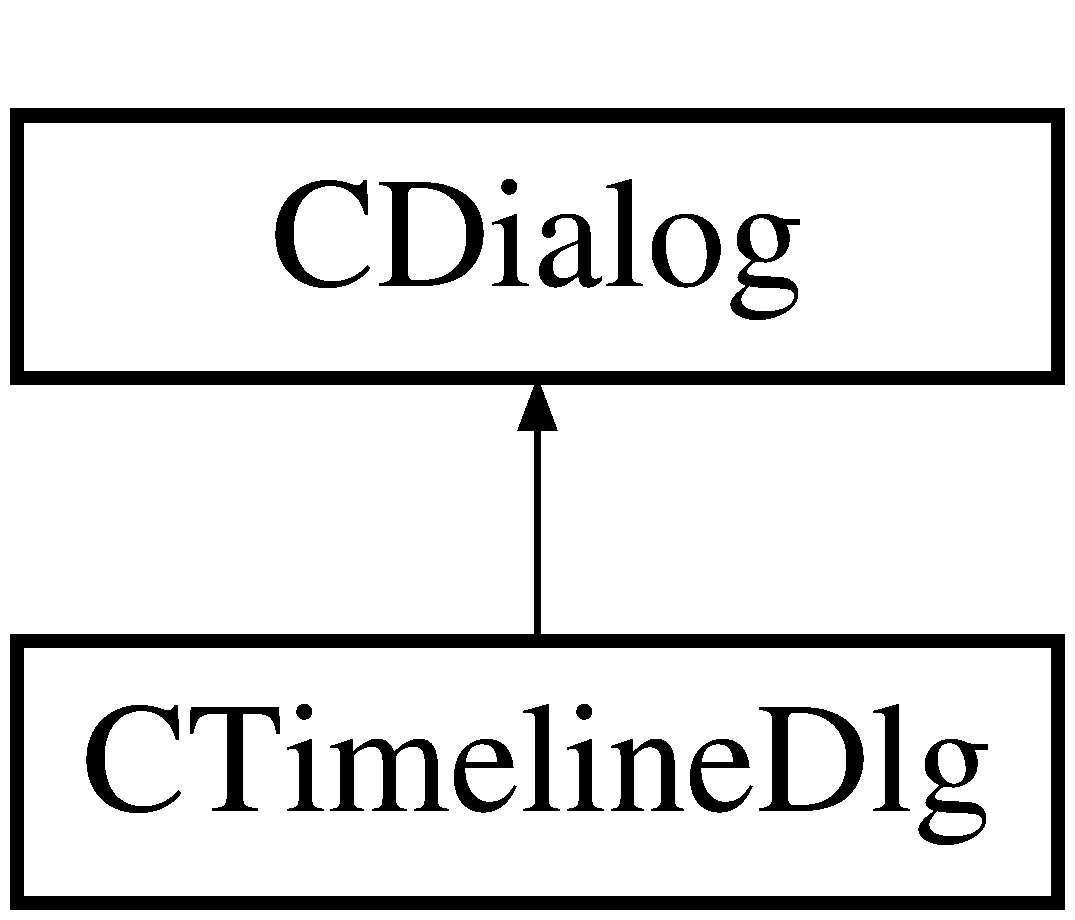
\includegraphics[height=2.000000cm]{class_c_timeline_dlg}
\end{center}
\end{figure}
\subsection*{Public Types}
\begin{DoxyCompactItemize}
\item 
\hypertarget{class_c_timeline_dlg_a330aa61151bda4840b8b241bca03793b}{enum \{ {\bfseries I\+D\+D} = I\+D\+D\+\_\+\+T\+I\+M\+E\+L\+I\+N\+E\+D\+L\+G
 \}}\label{class_c_timeline_dlg_a330aa61151bda4840b8b241bca03793b}

\end{DoxyCompactItemize}
\subsection*{Public Member Functions}
\begin{DoxyCompactItemize}
\item 
\hyperlink{class_c_timeline_dlg_a223084ec9e733c204098c759514ffad8}{C\+Timeline\+Dlg} (C\+Wnd $\ast$p\+Parent=N\+U\+L\+L)
\begin{DoxyCompactList}\small\item\em Constructor. \end{DoxyCompactList}\item 
\hypertarget{class_c_timeline_dlg_afd8204d07f08a1c38cf6945216ea2d25}{virtual \hyperlink{class_c_timeline_dlg_afd8204d07f08a1c38cf6945216ea2d25}{$\sim$\+C\+Timeline\+Dlg} ()}\label{class_c_timeline_dlg_afd8204d07f08a1c38cf6945216ea2d25}

\begin{DoxyCompactList}\small\item\em Destructor. \end{DoxyCompactList}\item 
void \hyperlink{class_c_timeline_dlg_a52cb094ebeb1ac40f9109a4bd98651e1}{Set\+Timeline} (\hyperlink{class_c_timeline}{C\+Timeline} $\ast$timeline)
\begin{DoxyCompactList}\small\item\em Pass a timeline object to this dialog box class. \end{DoxyCompactList}\item 
\hypertarget{class_c_timeline_dlg_a26e970d2fc1c0017d7ff3f5ab4e9092e}{void \hyperlink{class_c_timeline_dlg_a26e970d2fc1c0017d7ff3f5ab4e9092e}{Take} ()}\label{class_c_timeline_dlg_a26e970d2fc1c0017d7ff3f5ab4e9092e}

\begin{DoxyCompactList}\small\item\em Transfer dialog values to the Timeline object. \end{DoxyCompactList}\end{DoxyCompactItemize}
\subsection*{Protected Member Functions}
\begin{DoxyCompactItemize}
\item 
virtual void \hyperlink{class_c_timeline_dlg_a25237f8bfd8a868aeeb00518e86248b0}{Do\+Data\+Exchange} (C\+Data\+Exchange $\ast$p\+D\+X)
\begin{DoxyCompactList}\small\item\em Exchange data between the dialog box and local variables. \end{DoxyCompactList}\end{DoxyCompactItemize}


\subsection{Detailed Description}
The timeline parameters dialog box. 

\subsection{Constructor \& Destructor Documentation}
\hypertarget{class_c_timeline_dlg_a223084ec9e733c204098c759514ffad8}{\index{C\+Timeline\+Dlg@{C\+Timeline\+Dlg}!C\+Timeline\+Dlg@{C\+Timeline\+Dlg}}
\index{C\+Timeline\+Dlg@{C\+Timeline\+Dlg}!C\+Timeline\+Dlg@{C\+Timeline\+Dlg}}
\subsubsection[{C\+Timeline\+Dlg}]{\setlength{\rightskip}{0pt plus 5cm}C\+Timeline\+Dlg\+::\+C\+Timeline\+Dlg (
\begin{DoxyParamCaption}
\item[{C\+Wnd $\ast$}]{p\+Parent = {\ttfamily NULL}}
\end{DoxyParamCaption}
)}}\label{class_c_timeline_dlg_a223084ec9e733c204098c759514ffad8}


Constructor. 


\begin{DoxyParams}{Parameters}
{\em p\+Parent} & Parent window or N\+U\+L\+L if none \\
\hline
\end{DoxyParams}


\subsection{Member Function Documentation}
\hypertarget{class_c_timeline_dlg_a25237f8bfd8a868aeeb00518e86248b0}{\index{C\+Timeline\+Dlg@{C\+Timeline\+Dlg}!Do\+Data\+Exchange@{Do\+Data\+Exchange}}
\index{Do\+Data\+Exchange@{Do\+Data\+Exchange}!C\+Timeline\+Dlg@{C\+Timeline\+Dlg}}
\subsubsection[{Do\+Data\+Exchange}]{\setlength{\rightskip}{0pt plus 5cm}void C\+Timeline\+Dlg\+::\+Do\+Data\+Exchange (
\begin{DoxyParamCaption}
\item[{C\+Data\+Exchange $\ast$}]{p\+D\+X}
\end{DoxyParamCaption}
)\hspace{0.3cm}{\ttfamily [protected]}, {\ttfamily [virtual]}}}\label{class_c_timeline_dlg_a25237f8bfd8a868aeeb00518e86248b0}


Exchange data between the dialog box and local variables. 


\begin{DoxyParams}{Parameters}
{\em p\+D\+X} & \\
\hline
\end{DoxyParams}
\hypertarget{class_c_timeline_dlg_a52cb094ebeb1ac40f9109a4bd98651e1}{\index{C\+Timeline\+Dlg@{C\+Timeline\+Dlg}!Set\+Timeline@{Set\+Timeline}}
\index{Set\+Timeline@{Set\+Timeline}!C\+Timeline\+Dlg@{C\+Timeline\+Dlg}}
\subsubsection[{Set\+Timeline}]{\setlength{\rightskip}{0pt plus 5cm}void C\+Timeline\+Dlg\+::\+Set\+Timeline (
\begin{DoxyParamCaption}
\item[{{\bf C\+Timeline} $\ast$}]{timeline}
\end{DoxyParamCaption}
)}}\label{class_c_timeline_dlg_a52cb094ebeb1ac40f9109a4bd98651e1}


Pass a timeline object to this dialog box class. 


\begin{DoxyParams}{Parameters}
{\em timeline} & The timeline object. \\
\hline
\end{DoxyParams}


The documentation for this class was generated from the following files\+:\begin{DoxyCompactItemize}
\item 
\hyperlink{_timeline_dlg_8h}{Timeline\+Dlg.\+h}\item 
\hyperlink{_timeline_dlg_8cpp}{Timeline\+Dlg.\+cpp}\end{DoxyCompactItemize}

\hypertarget{class_c_view_actors}{\section{C\+View\+Actors Class Reference}
\label{class_c_view_actors}\index{C\+View\+Actors@{C\+View\+Actors}}
}


Class that provides a view windows for actors.  




{\ttfamily \#include $<$View\+Actors.\+h$>$}

Inheritance diagram for C\+View\+Actors\+:\begin{figure}[H]
\begin{center}
\leavevmode
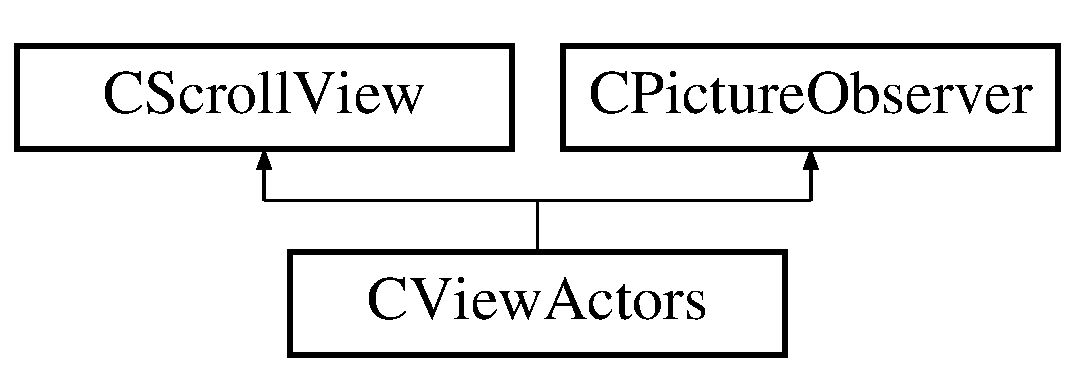
\includegraphics[height=2.000000cm]{class_c_view_actors}
\end{center}
\end{figure}
\subsection*{Public Member Functions}
\begin{DoxyCompactItemize}
\item 
void \hyperlink{class_c_view_actors_a6f68ae9e71f6a195502464bf34b3e724}{Set\+Main\+Frame} (\hyperlink{class_c_main_frame}{C\+Main\+Frame} $\ast$main\+Frame)
\begin{DoxyCompactList}\small\item\em Set the main\+Frame pointer. \end{DoxyCompactList}\item 
\hypertarget{class_c_view_actors_a5014f8c616850b8e874dee895b2ba698}{virtual void \hyperlink{class_c_view_actors_a5014f8c616850b8e874dee895b2ba698}{Update\+Observer} () override}\label{class_c_view_actors_a5014f8c616850b8e874dee895b2ba698}

\begin{DoxyCompactList}\small\item\em Force an update of this window when the picture changes. \end{DoxyCompactList}\item 
afx\+\_\+msg B\+O\+O\+L \hyperlink{class_c_view_actors_a561f4be212bd5df4a667c2cb0b23e472}{On\+Erase\+Bkgnd} (C\+D\+C $\ast$p\+D\+C)
\begin{DoxyCompactList}\small\item\em Erase the background. \end{DoxyCompactList}\end{DoxyCompactItemize}
\subsection*{Static Public Attributes}
\begin{DoxyCompactItemize}
\item 
\hypertarget{class_c_view_actors_a8bb27cbe8ae099abbed012adca884f1f}{static const int \hyperlink{class_c_view_actors_a8bb27cbe8ae099abbed012adca884f1f}{Width} = 150}\label{class_c_view_actors_a8bb27cbe8ae099abbed012adca884f1f}

\begin{DoxyCompactList}\small\item\em Width we want for this window. \end{DoxyCompactList}\end{DoxyCompactItemize}
\subsection*{Protected Member Functions}
\begin{DoxyCompactItemize}
\item 
\hyperlink{class_c_view_actors_aeff00d958ecea52760ec07c0420c4e28}{C\+View\+Actors} ()
\begin{DoxyCompactList}\small\item\em $\ast$/ \end{DoxyCompactList}\item 
\hypertarget{class_c_view_actors_a6e1aa1c82708dd805ac90c21b6d521e0}{virtual \hyperlink{class_c_view_actors_a6e1aa1c82708dd805ac90c21b6d521e0}{$\sim$\+C\+View\+Actors} ()}\label{class_c_view_actors_a6e1aa1c82708dd805ac90c21b6d521e0}

\begin{DoxyCompactList}\small\item\em Destructor. \end{DoxyCompactList}\item 
virtual void \hyperlink{class_c_view_actors_aa68465c2f13e487426508832a6355503}{On\+Draw} (C\+D\+C $\ast$p\+D\+C)
\begin{DoxyCompactList}\small\item\em Draw this window. \end{DoxyCompactList}\item 
\hypertarget{class_c_view_actors_aaf83b3647a42330c01be9067a6235d33}{virtual void \hyperlink{class_c_view_actors_aaf83b3647a42330c01be9067a6235d33}{On\+Initial\+Update} ()}\label{class_c_view_actors_aaf83b3647a42330c01be9067a6235d33}

\begin{DoxyCompactList}\small\item\em Handle the initial update for this window. \end{DoxyCompactList}\end{DoxyCompactItemize}


\subsection{Detailed Description}
Class that provides a view windows for actors. 

\subsection{Constructor \& Destructor Documentation}
\hypertarget{class_c_view_actors_aeff00d958ecea52760ec07c0420c4e28}{\index{C\+View\+Actors@{C\+View\+Actors}!C\+View\+Actors@{C\+View\+Actors}}
\index{C\+View\+Actors@{C\+View\+Actors}!C\+View\+Actors@{C\+View\+Actors}}
\subsubsection[{C\+View\+Actors}]{\setlength{\rightskip}{0pt plus 5cm}C\+View\+Actors\+::\+C\+View\+Actors (
\begin{DoxyParamCaption}
{}
\end{DoxyParamCaption}
)\hspace{0.3cm}{\ttfamily [protected]}}}\label{class_c_view_actors_aeff00d958ecea52760ec07c0420c4e28}


$\ast$/ 

Constructor 

\subsection{Member Function Documentation}
\hypertarget{class_c_view_actors_aa68465c2f13e487426508832a6355503}{\index{C\+View\+Actors@{C\+View\+Actors}!On\+Draw@{On\+Draw}}
\index{On\+Draw@{On\+Draw}!C\+View\+Actors@{C\+View\+Actors}}
\subsubsection[{On\+Draw}]{\setlength{\rightskip}{0pt plus 5cm}void C\+View\+Actors\+::\+On\+Draw (
\begin{DoxyParamCaption}
\item[{C\+D\+C $\ast$}]{p\+D\+C}
\end{DoxyParamCaption}
)\hspace{0.3cm}{\ttfamily [protected]}, {\ttfamily [virtual]}}}\label{class_c_view_actors_aa68465c2f13e487426508832a6355503}


Draw this window. 


\begin{DoxyParams}{Parameters}
{\em p\+D\+C} & Device context \\
\hline
\end{DoxyParams}
\hypertarget{class_c_view_actors_a561f4be212bd5df4a667c2cb0b23e472}{\index{C\+View\+Actors@{C\+View\+Actors}!On\+Erase\+Bkgnd@{On\+Erase\+Bkgnd}}
\index{On\+Erase\+Bkgnd@{On\+Erase\+Bkgnd}!C\+View\+Actors@{C\+View\+Actors}}
\subsubsection[{On\+Erase\+Bkgnd}]{\setlength{\rightskip}{0pt plus 5cm}B\+O\+O\+L C\+View\+Actors\+::\+On\+Erase\+Bkgnd (
\begin{DoxyParamCaption}
\item[{C\+D\+C $\ast$}]{p\+D\+C}
\end{DoxyParamCaption}
)}}\label{class_c_view_actors_a561f4be212bd5df4a667c2cb0b23e472}


Erase the background. 

This is disabled to eliminate flicker 
\begin{DoxyParams}{Parameters}
{\em p\+D\+C} & Device context \\
\hline
\end{DoxyParams}
\begin{DoxyReturn}{Returns}
F\+A\+L\+S\+E 
\end{DoxyReturn}
\hypertarget{class_c_view_actors_a6f68ae9e71f6a195502464bf34b3e724}{\index{C\+View\+Actors@{C\+View\+Actors}!Set\+Main\+Frame@{Set\+Main\+Frame}}
\index{Set\+Main\+Frame@{Set\+Main\+Frame}!C\+View\+Actors@{C\+View\+Actors}}
\subsubsection[{Set\+Main\+Frame}]{\setlength{\rightskip}{0pt plus 5cm}void C\+View\+Actors\+::\+Set\+Main\+Frame (
\begin{DoxyParamCaption}
\item[{{\bf C\+Main\+Frame} $\ast$}]{main\+Frame}
\end{DoxyParamCaption}
)\hspace{0.3cm}{\ttfamily [inline]}}}\label{class_c_view_actors_a6f68ae9e71f6a195502464bf34b3e724}


Set the main\+Frame pointer. 


\begin{DoxyParams}{Parameters}
{\em main\+Frame} & Pointer to the \hyperlink{class_c_main_frame}{C\+Main\+Frame} window \\
\hline
\end{DoxyParams}


The documentation for this class was generated from the following files\+:\begin{DoxyCompactItemize}
\item 
\hyperlink{_view_actors_8h}{View\+Actors.\+h}\item 
\hyperlink{_view_actors_8cpp}{View\+Actors.\+cpp}\end{DoxyCompactItemize}

\hypertarget{class_c_view_edit}{\section{C\+View\+Edit Class Reference}
\label{class_c_view_edit}\index{C\+View\+Edit@{C\+View\+Edit}}
}


View class the provides a window for editing our pixture.  




{\ttfamily \#include $<$View\+Edit.\+h$>$}

Inheritance diagram for C\+View\+Edit\+:\begin{figure}[H]
\begin{center}
\leavevmode
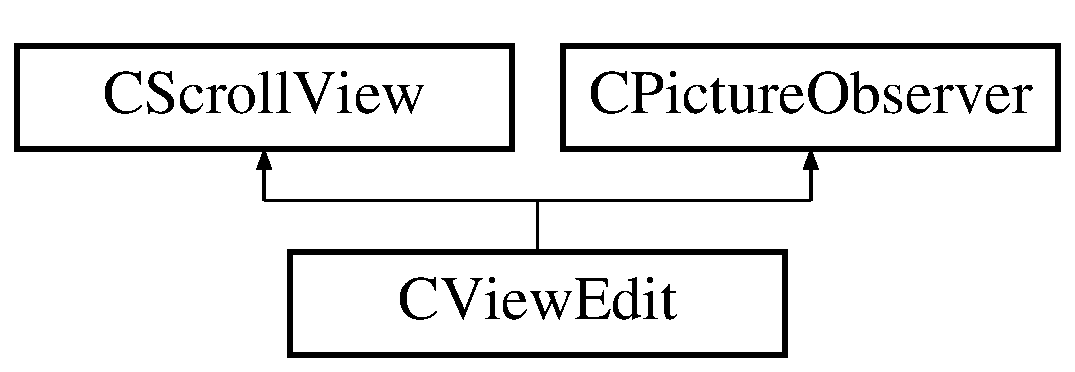
\includegraphics[height=2.000000cm]{class_c_view_edit}
\end{center}
\end{figure}
\subsection*{Public Member Functions}
\begin{DoxyCompactItemize}
\item 
\hypertarget{class_c_view_edit_a99fea37450207a1ffe8cf6b46ec2a11f}{\hyperlink{class_c_view_edit_a99fea37450207a1ffe8cf6b46ec2a11f}{C\+View\+Edit} ()}\label{class_c_view_edit_a99fea37450207a1ffe8cf6b46ec2a11f}

\begin{DoxyCompactList}\small\item\em Constructor. \end{DoxyCompactList}\item 
\hypertarget{class_c_view_edit_a968f16ef61489033c80ebe504017db3a}{virtual \hyperlink{class_c_view_edit_a968f16ef61489033c80ebe504017db3a}{$\sim$\+C\+View\+Edit} ()}\label{class_c_view_edit_a968f16ef61489033c80ebe504017db3a}

\begin{DoxyCompactList}\small\item\em Destructor. \end{DoxyCompactList}\item 
void \hyperlink{class_c_view_edit_a28bb793d43baba78e9b1c704b4f0e128}{Set\+Main\+Frame} (\hyperlink{class_c_main_frame}{C\+Main\+Frame} $\ast$main\+Frame)
\begin{DoxyCompactList}\small\item\em Set the main\+Frame pointer. \end{DoxyCompactList}\item 
\hypertarget{class_c_view_edit_ac2b73f20fe10a4a98096facde6450e5a}{virtual void \hyperlink{class_c_view_edit_ac2b73f20fe10a4a98096facde6450e5a}{Update\+Observer} () override}\label{class_c_view_edit_ac2b73f20fe10a4a98096facde6450e5a}

\begin{DoxyCompactList}\small\item\em Force an update of this window when the picture changes. \end{DoxyCompactList}\item 
afx\+\_\+msg B\+O\+O\+L \hyperlink{class_c_view_edit_a66446b22920245bb3b5c5735754d63cd}{On\+Erase\+Bkgnd} (C\+D\+C $\ast$p\+D\+C)
\begin{DoxyCompactList}\small\item\em Erase the background. \end{DoxyCompactList}\item 
afx\+\_\+msg void \hyperlink{class_c_view_edit_a0e77d59dd1ed299c933f660d9ff0cf7e}{On\+L\+Button\+Down} (U\+I\+N\+T n\+Flags, C\+Point point)
\begin{DoxyCompactList}\small\item\em Handle a left button click. \end{DoxyCompactList}\item 
afx\+\_\+msg void \hyperlink{class_c_view_edit_aba0b38ee4b51f9d98bc08ade92d9f051}{On\+Mouse\+Move} (U\+I\+N\+T n\+Flags, C\+Point point)
\begin{DoxyCompactList}\small\item\em Handle mouse movement. \end{DoxyCompactList}\end{DoxyCompactItemize}
\subsection*{Protected Member Functions}
\begin{DoxyCompactItemize}
\item 
virtual void \hyperlink{class_c_view_edit_a8cf50c2cebab5aaecda5ae6f7437cf38}{On\+Draw} (C\+D\+C $\ast$p\+D\+C)
\begin{DoxyCompactList}\small\item\em Drawing of the window. \end{DoxyCompactList}\item 
\hypertarget{class_c_view_edit_ac49ed2e9e35cd014c6539aaa4ac705f3}{virtual void \hyperlink{class_c_view_edit_ac49ed2e9e35cd014c6539aaa4ac705f3}{On\+Initial\+Update} ()}\label{class_c_view_edit_ac49ed2e9e35cd014c6539aaa4ac705f3}

\begin{DoxyCompactList}\small\item\em Handle initial update of the window. \end{DoxyCompactList}\end{DoxyCompactItemize}


\subsection{Detailed Description}
View class the provides a window for editing our pixture. 

\subsection{Member Function Documentation}
\hypertarget{class_c_view_edit_a8cf50c2cebab5aaecda5ae6f7437cf38}{\index{C\+View\+Edit@{C\+View\+Edit}!On\+Draw@{On\+Draw}}
\index{On\+Draw@{On\+Draw}!C\+View\+Edit@{C\+View\+Edit}}
\subsubsection[{On\+Draw}]{\setlength{\rightskip}{0pt plus 5cm}void C\+View\+Edit\+::\+On\+Draw (
\begin{DoxyParamCaption}
\item[{C\+D\+C $\ast$}]{p\+D\+C}
\end{DoxyParamCaption}
)\hspace{0.3cm}{\ttfamily [protected]}, {\ttfamily [virtual]}}}\label{class_c_view_edit_a8cf50c2cebab5aaecda5ae6f7437cf38}


Drawing of the window. 


\begin{DoxyParams}{Parameters}
{\em p\+D\+C} & the device context to draw on \\
\hline
\end{DoxyParams}
\hypertarget{class_c_view_edit_a66446b22920245bb3b5c5735754d63cd}{\index{C\+View\+Edit@{C\+View\+Edit}!On\+Erase\+Bkgnd@{On\+Erase\+Bkgnd}}
\index{On\+Erase\+Bkgnd@{On\+Erase\+Bkgnd}!C\+View\+Edit@{C\+View\+Edit}}
\subsubsection[{On\+Erase\+Bkgnd}]{\setlength{\rightskip}{0pt plus 5cm}B\+O\+O\+L C\+View\+Edit\+::\+On\+Erase\+Bkgnd (
\begin{DoxyParamCaption}
\item[{C\+D\+C $\ast$}]{p\+D\+C}
\end{DoxyParamCaption}
)}}\label{class_c_view_edit_a66446b22920245bb3b5c5735754d63cd}


Erase the background. 

This is disabled to eliminate flicker 
\begin{DoxyParams}{Parameters}
{\em p\+D\+C} & Device context \\
\hline
\end{DoxyParams}
\begin{DoxyReturn}{Returns}
F\+A\+L\+S\+E 
\end{DoxyReturn}
\hypertarget{class_c_view_edit_a0e77d59dd1ed299c933f660d9ff0cf7e}{\index{C\+View\+Edit@{C\+View\+Edit}!On\+L\+Button\+Down@{On\+L\+Button\+Down}}
\index{On\+L\+Button\+Down@{On\+L\+Button\+Down}!C\+View\+Edit@{C\+View\+Edit}}
\subsubsection[{On\+L\+Button\+Down}]{\setlength{\rightskip}{0pt plus 5cm}void C\+View\+Edit\+::\+On\+L\+Button\+Down (
\begin{DoxyParamCaption}
\item[{U\+I\+N\+T}]{n\+Flags, }
\item[{C\+Point}]{point}
\end{DoxyParamCaption}
)}}\label{class_c_view_edit_a0e77d59dd1ed299c933f660d9ff0cf7e}


Handle a left button click. 


\begin{DoxyParams}{Parameters}
{\em n\+Flags} & Flags that indicate status of the mouse buttons \\
\hline
{\em point} & The x,y location for the mouse click \\
\hline
\end{DoxyParams}
\hypertarget{class_c_view_edit_aba0b38ee4b51f9d98bc08ade92d9f051}{\index{C\+View\+Edit@{C\+View\+Edit}!On\+Mouse\+Move@{On\+Mouse\+Move}}
\index{On\+Mouse\+Move@{On\+Mouse\+Move}!C\+View\+Edit@{C\+View\+Edit}}
\subsubsection[{On\+Mouse\+Move}]{\setlength{\rightskip}{0pt plus 5cm}void C\+View\+Edit\+::\+On\+Mouse\+Move (
\begin{DoxyParamCaption}
\item[{U\+I\+N\+T}]{n\+Flags, }
\item[{C\+Point}]{point}
\end{DoxyParamCaption}
)}}\label{class_c_view_edit_aba0b38ee4b51f9d98bc08ade92d9f051}


Handle mouse movement. 


\begin{DoxyParams}{Parameters}
{\em n\+Flags} & Flags that indicate status of the mouse buttons \\
\hline
{\em point} & The x,y location for the mouse Handle mouse movement \\
\hline
{\em n\+Flags} & Flags that indicate status of the mouse buttons \\
\hline
{\em point} & The x,y location for the mouse \\
\hline
\end{DoxyParams}
\hypertarget{class_c_view_edit_a28bb793d43baba78e9b1c704b4f0e128}{\index{C\+View\+Edit@{C\+View\+Edit}!Set\+Main\+Frame@{Set\+Main\+Frame}}
\index{Set\+Main\+Frame@{Set\+Main\+Frame}!C\+View\+Edit@{C\+View\+Edit}}
\subsubsection[{Set\+Main\+Frame}]{\setlength{\rightskip}{0pt plus 5cm}void C\+View\+Edit\+::\+Set\+Main\+Frame (
\begin{DoxyParamCaption}
\item[{{\bf C\+Main\+Frame} $\ast$}]{main\+Frame}
\end{DoxyParamCaption}
)\hspace{0.3cm}{\ttfamily [inline]}}}\label{class_c_view_edit_a28bb793d43baba78e9b1c704b4f0e128}


Set the main\+Frame pointer. 


\begin{DoxyParams}{Parameters}
{\em main\+Frame} & Pointer to the \hyperlink{class_c_main_frame}{C\+Main\+Frame} window \\
\hline
\end{DoxyParams}


The documentation for this class was generated from the following files\+:\begin{DoxyCompactItemize}
\item 
\hyperlink{_view_edit_8h}{View\+Edit.\+h}\item 
\hyperlink{_view_edit_8cpp}{View\+Edit.\+cpp}\end{DoxyCompactItemize}

\hypertarget{class_c_view_timeline}{\section{C\+View\+Timeline Class Reference}
\label{class_c_view_timeline}\index{C\+View\+Timeline@{C\+View\+Timeline}}
}


View window for the animation timeline.  




{\ttfamily \#include $<$View\+Timeline.\+h$>$}

Inheritance diagram for C\+View\+Timeline\+:\begin{figure}[H]
\begin{center}
\leavevmode
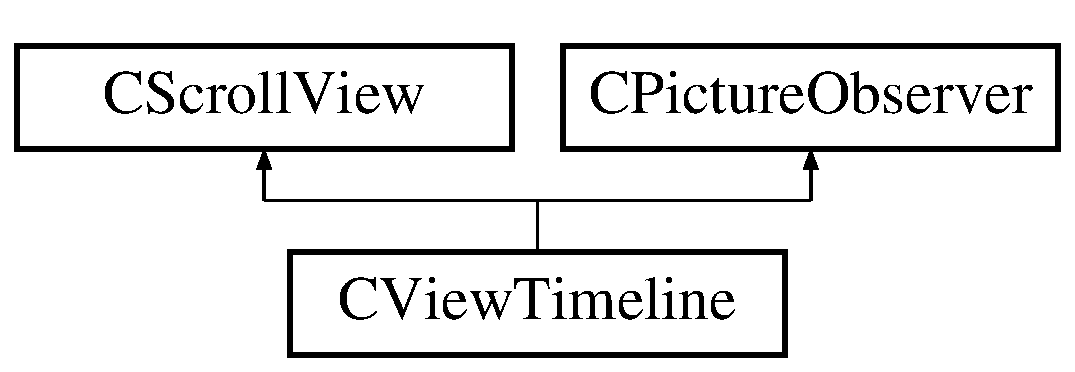
\includegraphics[height=2.000000cm]{class_c_view_timeline}
\end{center}
\end{figure}
\subsection*{Public Member Functions}
\begin{DoxyCompactItemize}
\item 
void \hyperlink{class_c_view_timeline_aba069993dd75712f340999345e791327}{Set\+Main\+Frame} (\hyperlink{class_c_main_frame}{C\+Main\+Frame} $\ast$main\+Frame)
\begin{DoxyCompactList}\small\item\em Set the main\+Frame pointer. \end{DoxyCompactList}\item 
\hypertarget{class_c_view_timeline_a21388abd4726fd3dbe02b6e2ea313369}{virtual void \hyperlink{class_c_view_timeline_a21388abd4726fd3dbe02b6e2ea313369}{Update\+Observer} () override}\label{class_c_view_timeline_a21388abd4726fd3dbe02b6e2ea313369}

\begin{DoxyCompactList}\small\item\em Force an update of this window when the picture changes. \end{DoxyCompactList}\item 
afx\+\_\+msg B\+O\+O\+L \hyperlink{class_c_view_timeline_a8328ae76e5f95d36b3ab7e8bbd8ef72f}{On\+Erase\+Bkgnd} (C\+D\+C $\ast$p\+D\+C)
\begin{DoxyCompactList}\small\item\em Erase the background. \end{DoxyCompactList}\item 
afx\+\_\+msg void \hyperlink{class_c_view_timeline_a851210b0ff7efb8446857c20c553d421}{On\+Mouse\+Move} (U\+I\+N\+T n\+Flags, C\+Point point)
\begin{DoxyCompactList}\small\item\em Handle mouse movement. \end{DoxyCompactList}\item 
afx\+\_\+msg void \hyperlink{class_c_view_timeline_a70a35fb411cff2bde0354e09d794038b}{On\+L\+Button\+Down} (U\+I\+N\+T n\+Flags, C\+Point point)
\begin{DoxyCompactList}\small\item\em Handle mouse click of left button. \end{DoxyCompactList}\item 
\hypertarget{class_c_view_timeline_acb22f2662a21152e607d17dbc293351c}{afx\+\_\+msg void \hyperlink{class_c_view_timeline_acb22f2662a21152e607d17dbc293351c}{On\+Edit\+Setkeyframe} ()}\label{class_c_view_timeline_acb22f2662a21152e607d17dbc293351c}

\begin{DoxyCompactList}\small\item\em Handle the Edit Set Keyframe menu option. \end{DoxyCompactList}\item 
\hypertarget{class_c_view_timeline_ab3eccb4a5bcd5ffa60442359b86e0597}{afx\+\_\+msg void \hyperlink{class_c_view_timeline_ab3eccb4a5bcd5ffa60442359b86e0597}{On\+Edit\+Deletekeyframe} ()}\label{class_c_view_timeline_ab3eccb4a5bcd5ffa60442359b86e0597}

\begin{DoxyCompactList}\small\item\em Handle a delete keyframe menu option. \end{DoxyCompactList}\item 
\hypertarget{class_c_view_timeline_a647b850c229507b28682d6b24e25e53c}{afx\+\_\+msg void \hyperlink{class_c_view_timeline_a647b850c229507b28682d6b24e25e53c}{On\+File\+Saveas} ()}\label{class_c_view_timeline_a647b850c229507b28682d6b24e25e53c}

\begin{DoxyCompactList}\small\item\em Handle the File/\+Save Animation As menu option. \end{DoxyCompactList}\item 
\hypertarget{class_c_view_timeline_a0679334f0c5d934467d14a831b768627}{afx\+\_\+msg void \hyperlink{class_c_view_timeline_a0679334f0c5d934467d14a831b768627}{On\+File\+Open32782} ()}\label{class_c_view_timeline_a0679334f0c5d934467d14a831b768627}

\begin{DoxyCompactList}\small\item\em Handle the File/\+Open Animation menu option. \end{DoxyCompactList}\end{DoxyCompactItemize}
\subsection*{Static Public Attributes}
\begin{DoxyCompactItemize}
\item 
\hypertarget{class_c_view_timeline_a6634479092090825e8c392902cf6c685}{static const int \hyperlink{class_c_view_timeline_a6634479092090825e8c392902cf6c685}{Height} = 90}\label{class_c_view_timeline_a6634479092090825e8c392902cf6c685}

\begin{DoxyCompactList}\small\item\em Height to make this window. \end{DoxyCompactList}\end{DoxyCompactItemize}
\subsection*{Protected Member Functions}
\begin{DoxyCompactItemize}
\item 
\hypertarget{class_c_view_timeline_aee8b6ebfaa9e299c65d6be0fc27b79f1}{\hyperlink{class_c_view_timeline_aee8b6ebfaa9e299c65d6be0fc27b79f1}{C\+View\+Timeline} ()}\label{class_c_view_timeline_aee8b6ebfaa9e299c65d6be0fc27b79f1}

\begin{DoxyCompactList}\small\item\em Constructor. \end{DoxyCompactList}\item 
\hypertarget{class_c_view_timeline_afec58a7cb0dfafd6c64c19e9e8a57842}{virtual \hyperlink{class_c_view_timeline_afec58a7cb0dfafd6c64c19e9e8a57842}{$\sim$\+C\+View\+Timeline} ()}\label{class_c_view_timeline_afec58a7cb0dfafd6c64c19e9e8a57842}

\begin{DoxyCompactList}\small\item\em Destructor. \end{DoxyCompactList}\item 
virtual void \hyperlink{class_c_view_timeline_a32f2ff1b162abc49f841e5dd6ddcb7df}{On\+Draw} (C\+D\+C $\ast$p\+D\+C)
\begin{DoxyCompactList}\small\item\em Draw this window. \end{DoxyCompactList}\item 
\hypertarget{class_c_view_timeline_a7996d31301f034cf9fa59e3d846c5fb5}{virtual void \hyperlink{class_c_view_timeline_a7996d31301f034cf9fa59e3d846c5fb5}{On\+Initial\+Update} ()}\label{class_c_view_timeline_a7996d31301f034cf9fa59e3d846c5fb5}

\begin{DoxyCompactList}\small\item\em Handle the initial update for this window. \end{DoxyCompactList}\end{DoxyCompactItemize}


\subsection{Detailed Description}
View window for the animation timeline. 

\subsection{Member Function Documentation}
\hypertarget{class_c_view_timeline_a32f2ff1b162abc49f841e5dd6ddcb7df}{\index{C\+View\+Timeline@{C\+View\+Timeline}!On\+Draw@{On\+Draw}}
\index{On\+Draw@{On\+Draw}!C\+View\+Timeline@{C\+View\+Timeline}}
\subsubsection[{On\+Draw}]{\setlength{\rightskip}{0pt plus 5cm}void C\+View\+Timeline\+::\+On\+Draw (
\begin{DoxyParamCaption}
\item[{C\+D\+C $\ast$}]{p\+D\+C}
\end{DoxyParamCaption}
)\hspace{0.3cm}{\ttfamily [protected]}, {\ttfamily [virtual]}}}\label{class_c_view_timeline_a32f2ff1b162abc49f841e5dd6ddcb7df}


Draw this window. 


\begin{DoxyParams}{Parameters}
{\em p\+D\+C} & Device context \\
\hline
\end{DoxyParams}
\hypertarget{class_c_view_timeline_a8328ae76e5f95d36b3ab7e8bbd8ef72f}{\index{C\+View\+Timeline@{C\+View\+Timeline}!On\+Erase\+Bkgnd@{On\+Erase\+Bkgnd}}
\index{On\+Erase\+Bkgnd@{On\+Erase\+Bkgnd}!C\+View\+Timeline@{C\+View\+Timeline}}
\subsubsection[{On\+Erase\+Bkgnd}]{\setlength{\rightskip}{0pt plus 5cm}B\+O\+O\+L C\+View\+Timeline\+::\+On\+Erase\+Bkgnd (
\begin{DoxyParamCaption}
\item[{C\+D\+C $\ast$}]{p\+D\+C}
\end{DoxyParamCaption}
)}}\label{class_c_view_timeline_a8328ae76e5f95d36b3ab7e8bbd8ef72f}


Erase the background. 

This is disabled to eliminate flicker 
\begin{DoxyParams}{Parameters}
{\em p\+D\+C} & Device context \\
\hline
\end{DoxyParams}
\begin{DoxyReturn}{Returns}
F\+A\+L\+S\+E 
\end{DoxyReturn}
\hypertarget{class_c_view_timeline_a70a35fb411cff2bde0354e09d794038b}{\index{C\+View\+Timeline@{C\+View\+Timeline}!On\+L\+Button\+Down@{On\+L\+Button\+Down}}
\index{On\+L\+Button\+Down@{On\+L\+Button\+Down}!C\+View\+Timeline@{C\+View\+Timeline}}
\subsubsection[{On\+L\+Button\+Down}]{\setlength{\rightskip}{0pt plus 5cm}void C\+View\+Timeline\+::\+On\+L\+Button\+Down (
\begin{DoxyParamCaption}
\item[{U\+I\+N\+T}]{n\+Flags, }
\item[{C\+Point}]{point}
\end{DoxyParamCaption}
)}}\label{class_c_view_timeline_a70a35fb411cff2bde0354e09d794038b}


Handle mouse click of left button. 


\begin{DoxyParams}{Parameters}
{\em n\+Flags} & Flags associated with the mouse movement \\
\hline
{\em point} & Current mouse location \\
\hline
\end{DoxyParams}
\hypertarget{class_c_view_timeline_a851210b0ff7efb8446857c20c553d421}{\index{C\+View\+Timeline@{C\+View\+Timeline}!On\+Mouse\+Move@{On\+Mouse\+Move}}
\index{On\+Mouse\+Move@{On\+Mouse\+Move}!C\+View\+Timeline@{C\+View\+Timeline}}
\subsubsection[{On\+Mouse\+Move}]{\setlength{\rightskip}{0pt plus 5cm}void C\+View\+Timeline\+::\+On\+Mouse\+Move (
\begin{DoxyParamCaption}
\item[{U\+I\+N\+T}]{n\+Flags, }
\item[{C\+Point}]{point}
\end{DoxyParamCaption}
)}}\label{class_c_view_timeline_a851210b0ff7efb8446857c20c553d421}


Handle mouse movement. 


\begin{DoxyParams}{Parameters}
{\em n\+Flags} & Flags associated with the mouse movement \\
\hline
{\em point} & Current mouse location \\
\hline
\end{DoxyParams}
\hypertarget{class_c_view_timeline_aba069993dd75712f340999345e791327}{\index{C\+View\+Timeline@{C\+View\+Timeline}!Set\+Main\+Frame@{Set\+Main\+Frame}}
\index{Set\+Main\+Frame@{Set\+Main\+Frame}!C\+View\+Timeline@{C\+View\+Timeline}}
\subsubsection[{Set\+Main\+Frame}]{\setlength{\rightskip}{0pt plus 5cm}void C\+View\+Timeline\+::\+Set\+Main\+Frame (
\begin{DoxyParamCaption}
\item[{{\bf C\+Main\+Frame} $\ast$}]{main\+Frame}
\end{DoxyParamCaption}
)\hspace{0.3cm}{\ttfamily [inline]}}}\label{class_c_view_timeline_aba069993dd75712f340999345e791327}


Set the main\+Frame pointer. 


\begin{DoxyParams}{Parameters}
{\em main\+Frame} & Pointer to the \hyperlink{class_c_main_frame}{C\+Main\+Frame} window \\
\hline
\end{DoxyParams}


The documentation for this class was generated from the following files\+:\begin{DoxyCompactItemize}
\item 
\hyperlink{_view_timeline_8h}{View\+Timeline.\+h}\item 
\hyperlink{_view_timeline_8cpp}{View\+Timeline.\+cpp}\end{DoxyCompactItemize}

\hypertarget{class_c_view_top}{\section{C\+View\+Top Class Reference}
\label{class_c_view_top}\index{C\+View\+Top@{C\+View\+Top}}
}


Top of the screen view.  




{\ttfamily \#include $<$View\+Top.\+h$>$}

Inheritance diagram for C\+View\+Top\+:\begin{figure}[H]
\begin{center}
\leavevmode
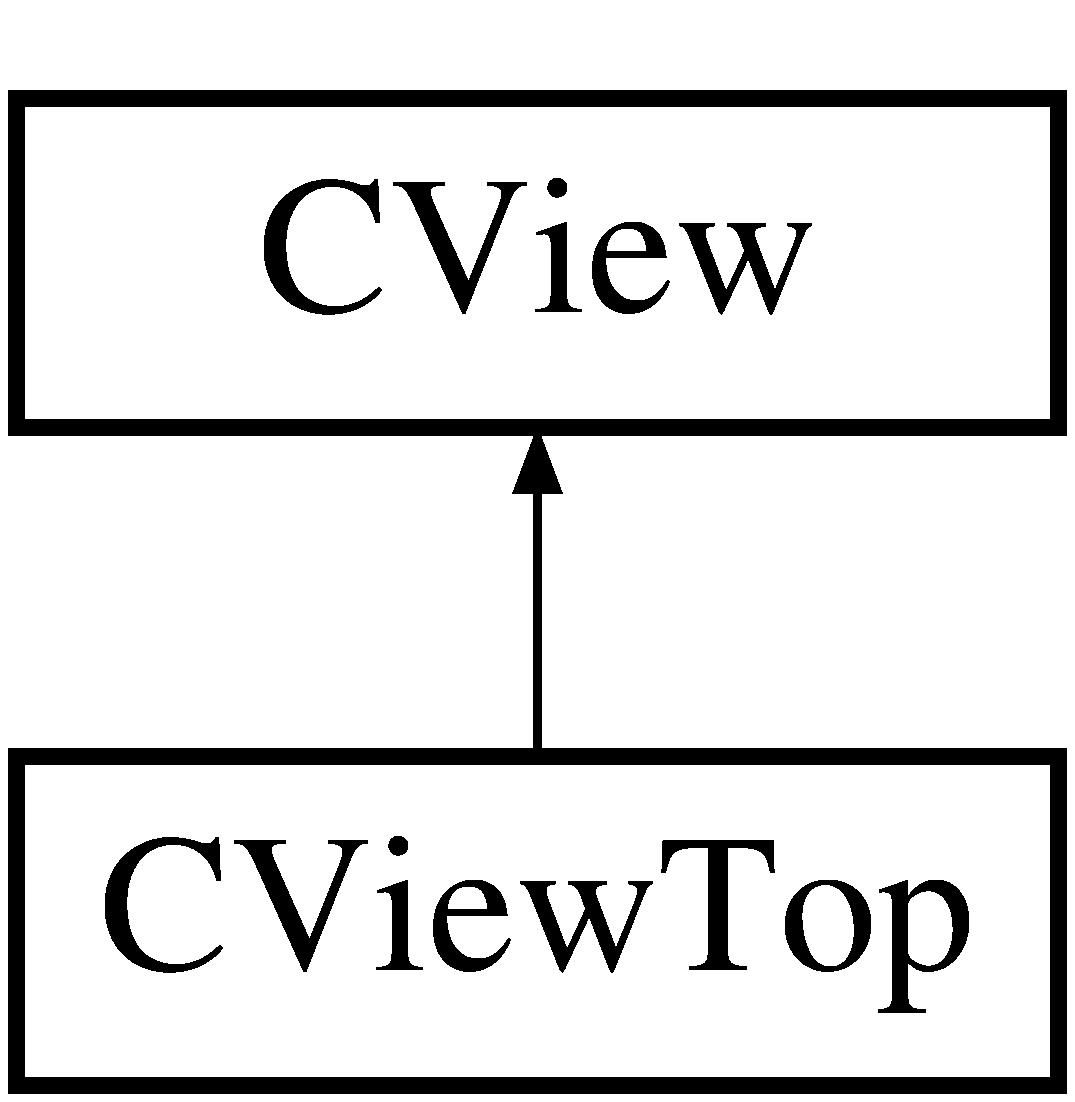
\includegraphics[height=2.000000cm]{class_c_view_top}
\end{center}
\end{figure}
\subsection*{Public Member Functions}
\begin{DoxyCompactItemize}
\item 
virtual void \hyperlink{class_c_view_top_ac4b8af93a75df56478f39feff289f6a6}{On\+Draw} (C\+D\+C $\ast$p\+D\+C)
\begin{DoxyCompactList}\small\item\em Drawing for this view. \end{DoxyCompactList}\item 
\hyperlink{class_c_view_edit}{C\+View\+Edit} $\ast$ \hyperlink{class_c_view_top_a775f50213ecac76ac57016bc402de42a}{Get\+View\+Edit} ()
\begin{DoxyCompactList}\small\item\em Get the View\+Edit window. \end{DoxyCompactList}\item 
\hyperlink{class_c_view_actors}{C\+View\+Actors} $\ast$ \hyperlink{class_c_view_top_a2057cf44f1f7a789b33e2ef8444b6db8}{Get\+View\+Actors} ()
\begin{DoxyCompactList}\small\item\em Get the View\+Actors window. \end{DoxyCompactList}\item 
afx\+\_\+msg int \hyperlink{class_c_view_top_a7e4cad13135855a66719ecb49a8ad3fc}{On\+Create} (L\+P\+C\+R\+E\+A\+T\+E\+S\+T\+R\+U\+C\+T lp\+Create\+Struct)
\begin{DoxyCompactList}\small\item\em Handle a C\+R\+E\+A\+T\+E message for this window. \end{DoxyCompactList}\item 
afx\+\_\+msg void \hyperlink{class_c_view_top_a171e02fdf1bef80245bbc37d77819f14}{On\+Size} (U\+I\+N\+T n\+Type, int cx, int cy)
\begin{DoxyCompactList}\small\item\em Handle a new size message. \end{DoxyCompactList}\end{DoxyCompactItemize}
\subsection*{Protected Member Functions}
\begin{DoxyCompactItemize}
\item 
\hypertarget{class_c_view_top_a4cee9890cf66890c3cd79efdedf92d1b}{\hyperlink{class_c_view_top_a4cee9890cf66890c3cd79efdedf92d1b}{C\+View\+Top} ()}\label{class_c_view_top_a4cee9890cf66890c3cd79efdedf92d1b}

\begin{DoxyCompactList}\small\item\em Constructor. \end{DoxyCompactList}\item 
\hypertarget{class_c_view_top_ad08e0ef0c01e33bb0278dc595467ad8c}{virtual \hyperlink{class_c_view_top_ad08e0ef0c01e33bb0278dc595467ad8c}{$\sim$\+C\+View\+Top} ()}\label{class_c_view_top_ad08e0ef0c01e33bb0278dc595467ad8c}

\begin{DoxyCompactList}\small\item\em Destructor. \end{DoxyCompactList}\end{DoxyCompactItemize}


\subsection{Detailed Description}
Top of the screen view. 

This class creates a view that contains a splitter so we can split the top window horizontally. 

\subsection{Member Function Documentation}
\hypertarget{class_c_view_top_a2057cf44f1f7a789b33e2ef8444b6db8}{\index{C\+View\+Top@{C\+View\+Top}!Get\+View\+Actors@{Get\+View\+Actors}}
\index{Get\+View\+Actors@{Get\+View\+Actors}!C\+View\+Top@{C\+View\+Top}}
\subsubsection[{Get\+View\+Actors}]{\setlength{\rightskip}{0pt plus 5cm}{\bf C\+View\+Actors}$\ast$ C\+View\+Top\+::\+Get\+View\+Actors (
\begin{DoxyParamCaption}
{}
\end{DoxyParamCaption}
)\hspace{0.3cm}{\ttfamily [inline]}}}\label{class_c_view_top_a2057cf44f1f7a789b33e2ef8444b6db8}


Get the View\+Actors window. 

\begin{DoxyReturn}{Returns}
Pointer to View\+Actors window 
\end{DoxyReturn}
\hypertarget{class_c_view_top_a775f50213ecac76ac57016bc402de42a}{\index{C\+View\+Top@{C\+View\+Top}!Get\+View\+Edit@{Get\+View\+Edit}}
\index{Get\+View\+Edit@{Get\+View\+Edit}!C\+View\+Top@{C\+View\+Top}}
\subsubsection[{Get\+View\+Edit}]{\setlength{\rightskip}{0pt plus 5cm}{\bf C\+View\+Edit}$\ast$ C\+View\+Top\+::\+Get\+View\+Edit (
\begin{DoxyParamCaption}
{}
\end{DoxyParamCaption}
)\hspace{0.3cm}{\ttfamily [inline]}}}\label{class_c_view_top_a775f50213ecac76ac57016bc402de42a}


Get the View\+Edit window. 

\begin{DoxyReturn}{Returns}
Pointer to View\+Edit window 
\end{DoxyReturn}
\hypertarget{class_c_view_top_a7e4cad13135855a66719ecb49a8ad3fc}{\index{C\+View\+Top@{C\+View\+Top}!On\+Create@{On\+Create}}
\index{On\+Create@{On\+Create}!C\+View\+Top@{C\+View\+Top}}
\subsubsection[{On\+Create}]{\setlength{\rightskip}{0pt plus 5cm}int C\+View\+Top\+::\+On\+Create (
\begin{DoxyParamCaption}
\item[{L\+P\+C\+R\+E\+A\+T\+E\+S\+T\+R\+U\+C\+T}]{lp\+Create\+Struct}
\end{DoxyParamCaption}
)}}\label{class_c_view_top_a7e4cad13135855a66719ecb49a8ad3fc}


Handle a C\+R\+E\+A\+T\+E message for this window. 


\begin{DoxyParams}{Parameters}
{\em lp\+Create\+Struct} & The creation parameter structure \\
\hline
\end{DoxyParams}
\begin{DoxyReturn}{Returns}
0 if successful 
\end{DoxyReturn}
\hypertarget{class_c_view_top_ac4b8af93a75df56478f39feff289f6a6}{\index{C\+View\+Top@{C\+View\+Top}!On\+Draw@{On\+Draw}}
\index{On\+Draw@{On\+Draw}!C\+View\+Top@{C\+View\+Top}}
\subsubsection[{On\+Draw}]{\setlength{\rightskip}{0pt plus 5cm}void C\+View\+Top\+::\+On\+Draw (
\begin{DoxyParamCaption}
\item[{C\+D\+C $\ast$}]{p\+D\+C}
\end{DoxyParamCaption}
)\hspace{0.3cm}{\ttfamily [virtual]}}}\label{class_c_view_top_ac4b8af93a75df56478f39feff289f6a6}


Drawing for this view. 


\begin{DoxyParams}{Parameters}
{\em p\+D\+C} & The device context \\
\hline
\end{DoxyParams}
\hypertarget{class_c_view_top_a171e02fdf1bef80245bbc37d77819f14}{\index{C\+View\+Top@{C\+View\+Top}!On\+Size@{On\+Size}}
\index{On\+Size@{On\+Size}!C\+View\+Top@{C\+View\+Top}}
\subsubsection[{On\+Size}]{\setlength{\rightskip}{0pt plus 5cm}void C\+View\+Top\+::\+On\+Size (
\begin{DoxyParamCaption}
\item[{U\+I\+N\+T}]{n\+Type, }
\item[{int}]{cx, }
\item[{int}]{cy}
\end{DoxyParamCaption}
)}}\label{class_c_view_top_a171e02fdf1bef80245bbc37d77819f14}


Handle a new size message. 


\begin{DoxyParams}{Parameters}
{\em n\+Type} & Type of size message \\
\hline
{\em cx} & New width \\
\hline
{\em cy} & New height \\
\hline
\end{DoxyParams}


The documentation for this class was generated from the following files\+:\begin{DoxyCompactItemize}
\item 
\hyperlink{_view_top_8h}{View\+Top.\+h}\item 
\hyperlink{_view_top_8cpp}{View\+Top.\+cpp}\end{DoxyCompactItemize}

\hypertarget{classxmlnode_1_1_c_xml_node}{\section{xmlnode\+:\+:C\+Xml\+Node Class Reference}
\label{classxmlnode_1_1_c_xml_node}\index{xmlnode\+::\+C\+Xml\+Node@{xmlnode\+::\+C\+Xml\+Node}}
}


A wrapper for msxml nodes.  




{\ttfamily \#include $<$Xml\+Node.\+h$>$}

\subsection*{Classes}
\begin{DoxyCompactItemize}
\item 
class \hyperlink{classxmlnode_1_1_c_xml_node_1_1_children}{Children}
\begin{DoxyCompactList}\small\item\em Representation of children to support iteration. \end{DoxyCompactList}\item 
class \hyperlink{classxmlnode_1_1_c_xml_node_1_1_exception}{Exception}
\begin{DoxyCompactList}\small\item\em Exceptions for \hyperlink{classxmlnode_1_1_c_xml_node}{C\+Xml\+Node}. \end{DoxyCompactList}\item 
class \hyperlink{classxmlnode_1_1_c_xml_node_1_1_iterator}{Iterator}
\begin{DoxyCompactList}\small\item\em Support for iterating over the children of a node. \end{DoxyCompactList}\end{DoxyCompactItemize}
\subsection*{Public Member Functions}
\begin{DoxyCompactItemize}
\item 
\hyperlink{classxmlnode_1_1_c_xml_node_a0f05b63e034bb5620609a2020c591d55}{C\+Xml\+Node} ()
\begin{DoxyCompactList}\small\item\em Constructor. \end{DoxyCompactList}\item 
\hypertarget{classxmlnode_1_1_c_xml_node_ad3e072fa0d46c534c08f013405e051ae}{virtual \hyperlink{classxmlnode_1_1_c_xml_node_ad3e072fa0d46c534c08f013405e051ae}{$\sim$\+C\+Xml\+Node} ()}\label{classxmlnode_1_1_c_xml_node_ad3e072fa0d46c534c08f013405e051ae}

\begin{DoxyCompactList}\small\item\em Destructor. \end{DoxyCompactList}\item 
void \hyperlink{classxmlnode_1_1_c_xml_node_abfd7b791490e58aac7091b78e36bd24b}{Open} (const std\+::wstring \&filename)
\begin{DoxyCompactList}\small\item\em Open a file as an X\+M\+L document. \end{DoxyCompactList}\item 
void \hyperlink{classxmlnode_1_1_c_xml_node_a7f4a7dee5a7de490507b9d0ed78dbab7}{Create} (const std\+::wstring \&rootname)
\begin{DoxyCompactList}\small\item\em Create an empty X\+M\+L document in this node. \end{DoxyCompactList}\item 
void \hyperlink{classxmlnode_1_1_c_xml_node_a0f83eef381fe59726503e0fcb854661d}{Save} (const std\+::wstring \&filename)
\begin{DoxyCompactList}\small\item\em Save X\+M\+L document to a file. \end{DoxyCompactList}\item 
std\+::wstring \hyperlink{classxmlnode_1_1_c_xml_node_a700c3de386529eab05b185c38b17fd51}{Get\+X\+M\+L} ()
\begin{DoxyCompactList}\small\item\em Obtain the created X\+M\+L as a string. \end{DoxyCompactList}\item 
std\+::wstring \hyperlink{classxmlnode_1_1_c_xml_node_a90fbe5f25e67b82a0d3caf7bb5d46791}{Get\+Name} () const 
\begin{DoxyCompactList}\small\item\em The node name. \end{DoxyCompactList}\item 
D\+O\+M\+Node\+Type \hyperlink{classxmlnode_1_1_c_xml_node_a85b513f8617fb75a721c646b62be95ab}{Get\+Type} () const 
\begin{DoxyCompactList}\small\item\em The node type. \end{DoxyCompactList}\item 
std\+::wstring \hyperlink{classxmlnode_1_1_c_xml_node_a383ef3eb35e61fc6a5a8889ed67f2a33}{Get\+Value} () const 
\begin{DoxyCompactList}\small\item\em Get the node value. \end{DoxyCompactList}\item 
int \hyperlink{classxmlnode_1_1_c_xml_node_a9eacb7b529d5690449fc0981b679edac}{Get\+Int\+Value} () const 
\begin{DoxyCompactList}\small\item\em Get the node value. \end{DoxyCompactList}\item 
double \hyperlink{classxmlnode_1_1_c_xml_node_a1ab9947b3e2f3aba9b6f044779b7e25b}{Get\+Double\+Value} () const 
\begin{DoxyCompactList}\small\item\em Get the node value. \end{DoxyCompactList}\item 
std\+::shared\+\_\+ptr$<$ \hyperlink{classxmlnode_1_1_c_xml_node}{C\+Xml\+Node} $>$ \hyperlink{classxmlnode_1_1_c_xml_node_aa571e6a48132a260420a077dde31168f}{Get\+Attribute} (const std\+::wstring \&name)
\begin{DoxyCompactList}\small\item\em Get an attribute. \end{DoxyCompactList}\item 
std\+::wstring \hyperlink{classxmlnode_1_1_c_xml_node_ac4b635b102a0ba6c0f64d047fd27f2a1}{Get\+Attribute\+Value} (const std\+::wstring \&name, const std\+::wstring \&def)
\begin{DoxyCompactList}\small\item\em Get the value of an attribute. \end{DoxyCompactList}\item 
int \hyperlink{classxmlnode_1_1_c_xml_node_a870618bd8862b8f3834613f469e56d25}{Get\+Attribute\+Int\+Value} (const std\+::wstring \&name, int def)
\begin{DoxyCompactList}\small\item\em Get the value of an attribute. \end{DoxyCompactList}\item 
double \hyperlink{classxmlnode_1_1_c_xml_node_a69fcfbe75f19450db6fe72908ce7c52e}{Get\+Attribute\+Double\+Value} (const std\+::wstring \&name, double def)
\begin{DoxyCompactList}\small\item\em Get the value of an attribute. \end{DoxyCompactList}\item 
void \hyperlink{classxmlnode_1_1_c_xml_node_ac2543c8908d29642f70c9ce437475bf1}{Set\+Attribute} (const std\+::wstring \&name, const std\+::wstring \&val)
\begin{DoxyCompactList}\small\item\em Set an attribute on this node. \end{DoxyCompactList}\item 
void \hyperlink{classxmlnode_1_1_c_xml_node_a6771d1de541ffefcf8a4fcd809b12b62}{Set\+Attribute} (const std\+::wstring \&name, int val)
\begin{DoxyCompactList}\small\item\em Set an attribute on this node. \end{DoxyCompactList}\item 
void \hyperlink{classxmlnode_1_1_c_xml_node_a1bfd97eb8de5e6f769b5ed29039b91ea}{Set\+Attribute} (const std\+::wstring \&name, double val)
\begin{DoxyCompactList}\small\item\em Set an attribute on this node. \end{DoxyCompactList}\item 
std\+::shared\+\_\+ptr$<$ \hyperlink{classxmlnode_1_1_c_xml_node}{C\+Xml\+Node} $>$ \hyperlink{classxmlnode_1_1_c_xml_node_ac5700bda1faebcbe5bb042e043ea60be}{Get\+Child} (int n)
\begin{DoxyCompactList}\small\item\em Get a child node of this node by index. \end{DoxyCompactList}\item 
\hyperlink{classxmlnode_1_1_c_xml_node_1_1_children}{Children} \hyperlink{classxmlnode_1_1_c_xml_node_a03f86570ca40d4cc09c3e1841939a9d0}{Get\+Children} ()
\begin{DoxyCompactList}\small\item\em Get the children of this node. \end{DoxyCompactList}\item 
int \hyperlink{classxmlnode_1_1_c_xml_node_ab455bd55e7f3dbd550e81d7fe293d146}{Get\+Num\+Children} ()
\begin{DoxyCompactList}\small\item\em Number of children of this node. \end{DoxyCompactList}\item 
std\+::shared\+\_\+ptr$<$ \hyperlink{classxmlnode_1_1_c_xml_node}{C\+Xml\+Node} $>$ \hyperlink{classxmlnode_1_1_c_xml_node_a7227a654358ffb87a2a57c165dee509c}{Add\+Child} (const std\+::wstring \&name)
\begin{DoxyCompactList}\small\item\em Add a child node to this node. \end{DoxyCompactList}\end{DoxyCompactItemize}
\subsection*{Static Public Member Functions}
\begin{DoxyCompactItemize}
\item 
static std\+::shared\+\_\+ptr$<$ \hyperlink{classxmlnode_1_1_c_xml_node}{C\+Xml\+Node} $>$ \hyperlink{classxmlnode_1_1_c_xml_node_ad71ff87937ae943a9c11f5891d53d93b}{Open\+Document} (const std\+::wstring \&filename)
\begin{DoxyCompactList}\small\item\em Open an X\+M\+L document and return the document root node. \end{DoxyCompactList}\item 
static std\+::shared\+\_\+ptr$<$ \hyperlink{classxmlnode_1_1_c_xml_node}{C\+Xml\+Node} $>$ \hyperlink{classxmlnode_1_1_c_xml_node_ae50a4482c4ea73492001f91788945bb1}{Create\+Document} (const std\+::wstring \&rootname)
\begin{DoxyCompactList}\small\item\em Create an empty X\+M\+L document and return the document root node. \end{DoxyCompactList}\end{DoxyCompactItemize}


\subsection{Detailed Description}
A wrapper for msxml nodes. 

M\+S\+X\+M\+L was designed to be used by a variety of languages, including C++, C\#, and Visual Basic. Consequently, it is a compromise that is very cumbersome to use. This class is designed to simplify the process considerably.

All an X\+M\+L document is a tree of nodes. This class represents nodes in that tree and the root node represents that underlying document. This class can be used to both create and load X\+M\+L documents.

\begin{DoxyVersion}{Version}
1.\+01 07-\/16-\/2014 Initial development 

1.\+02 07-\/17-\/2014 Namespace, added Get\+X\+M\+L, added tests 

1.\+03 07-\/17-\/2014 Exceptions 
\end{DoxyVersion}


\subsection{Constructor \& Destructor Documentation}
\hypertarget{classxmlnode_1_1_c_xml_node_a0f05b63e034bb5620609a2020c591d55}{\index{xmlnode\+::\+C\+Xml\+Node@{xmlnode\+::\+C\+Xml\+Node}!C\+Xml\+Node@{C\+Xml\+Node}}
\index{C\+Xml\+Node@{C\+Xml\+Node}!xmlnode\+::\+C\+Xml\+Node@{xmlnode\+::\+C\+Xml\+Node}}
\subsubsection[{C\+Xml\+Node}]{\setlength{\rightskip}{0pt plus 5cm}C\+Xml\+Node\+::\+C\+Xml\+Node (
\begin{DoxyParamCaption}
{}
\end{DoxyParamCaption}
)}}\label{classxmlnode_1_1_c_xml_node_a0f05b63e034bb5620609a2020c591d55}


Constructor. 

Creates an empty \hyperlink{classxmlnode_1_1_c_xml_node}{C\+Xml\+Node} with no attached X\+M\+L document. You can then call either Open or Create on the node. However, the preferred method is to use the static member functions Open\+Document and Create\+Document. 

\subsection{Member Function Documentation}
\hypertarget{classxmlnode_1_1_c_xml_node_a7227a654358ffb87a2a57c165dee509c}{\index{xmlnode\+::\+C\+Xml\+Node@{xmlnode\+::\+C\+Xml\+Node}!Add\+Child@{Add\+Child}}
\index{Add\+Child@{Add\+Child}!xmlnode\+::\+C\+Xml\+Node@{xmlnode\+::\+C\+Xml\+Node}}
\subsubsection[{Add\+Child}]{\setlength{\rightskip}{0pt plus 5cm}std\+::shared\+\_\+ptr$<$ {\bf C\+Xml\+Node} $>$ C\+Xml\+Node\+::\+Add\+Child (
\begin{DoxyParamCaption}
\item[{const std\+::wstring \&}]{name}
\end{DoxyParamCaption}
)}}\label{classxmlnode_1_1_c_xml_node_a7227a654358ffb87a2a57c165dee509c}


Add a child node to this node. 


\begin{DoxyParams}{Parameters}
{\em name} & Name of the child node. \\
\hline
\end{DoxyParams}
\begin{DoxyReturn}{Returns}
\hyperlink{classxmlnode_1_1_c_xml_node}{C\+Xml\+Node} object for the child node. 
\end{DoxyReturn}
\hypertarget{classxmlnode_1_1_c_xml_node_a7f4a7dee5a7de490507b9d0ed78dbab7}{\index{xmlnode\+::\+C\+Xml\+Node@{xmlnode\+::\+C\+Xml\+Node}!Create@{Create}}
\index{Create@{Create}!xmlnode\+::\+C\+Xml\+Node@{xmlnode\+::\+C\+Xml\+Node}}
\subsubsection[{Create}]{\setlength{\rightskip}{0pt plus 5cm}void C\+Xml\+Node\+::\+Create (
\begin{DoxyParamCaption}
\item[{const std\+::wstring \&}]{rootname}
\end{DoxyParamCaption}
)}}\label{classxmlnode_1_1_c_xml_node_a7f4a7dee5a7de490507b9d0ed78dbab7}


Create an empty X\+M\+L document in this node. 


\begin{DoxyParams}{Parameters}
{\em rootname} & The name for the root node. \\
\hline
\end{DoxyParams}
\hypertarget{classxmlnode_1_1_c_xml_node_ae50a4482c4ea73492001f91788945bb1}{\index{xmlnode\+::\+C\+Xml\+Node@{xmlnode\+::\+C\+Xml\+Node}!Create\+Document@{Create\+Document}}
\index{Create\+Document@{Create\+Document}!xmlnode\+::\+C\+Xml\+Node@{xmlnode\+::\+C\+Xml\+Node}}
\subsubsection[{Create\+Document}]{\setlength{\rightskip}{0pt plus 5cm}std\+::shared\+\_\+ptr$<$ {\bf C\+Xml\+Node} $>$ C\+Xml\+Node\+::\+Create\+Document (
\begin{DoxyParamCaption}
\item[{const std\+::wstring \&}]{rootname}
\end{DoxyParamCaption}
)\hspace{0.3cm}{\ttfamily [static]}}}\label{classxmlnode_1_1_c_xml_node_ae50a4482c4ea73492001f91788945bb1}


Create an empty X\+M\+L document and return the document root node. 


\begin{DoxyParams}{Parameters}
{\em rootname} & The name for the root node. \\
\hline
\end{DoxyParams}
\begin{DoxyReturn}{Returns}
Document root node 
\end{DoxyReturn}
\hypertarget{classxmlnode_1_1_c_xml_node_aa571e6a48132a260420a077dde31168f}{\index{xmlnode\+::\+C\+Xml\+Node@{xmlnode\+::\+C\+Xml\+Node}!Get\+Attribute@{Get\+Attribute}}
\index{Get\+Attribute@{Get\+Attribute}!xmlnode\+::\+C\+Xml\+Node@{xmlnode\+::\+C\+Xml\+Node}}
\subsubsection[{Get\+Attribute}]{\setlength{\rightskip}{0pt plus 5cm}std\+::shared\+\_\+ptr$<$ {\bf C\+Xml\+Node} $>$ C\+Xml\+Node\+::\+Get\+Attribute (
\begin{DoxyParamCaption}
\item[{const std\+::wstring \&}]{name}
\end{DoxyParamCaption}
)}}\label{classxmlnode_1_1_c_xml_node_aa571e6a48132a260420a077dde31168f}


Get an attribute. 

This returns a \hyperlink{classxmlnode_1_1_c_xml_node}{C\+Xml\+Node} object that is the attribute. You an then use the Get\+Value function to get the value of the attribute.

Calls to this function create a \hyperlink{classxmlnode_1_1_c_xml_node}{C\+Xml\+Node} object as a wrapper for the underlying attribute. Subsequent calls for the same attribute will return a different object.


\begin{DoxyParams}{Parameters}
{\em name} & Attribute name \\
\hline
\end{DoxyParams}
\begin{DoxyReturn}{Returns}
Attribute as a \hyperlink{classxmlnode_1_1_c_xml_node}{C\+Xml\+Node} object or null if attribute does not exist. 
\end{DoxyReturn}
\hypertarget{classxmlnode_1_1_c_xml_node_a69fcfbe75f19450db6fe72908ce7c52e}{\index{xmlnode\+::\+C\+Xml\+Node@{xmlnode\+::\+C\+Xml\+Node}!Get\+Attribute\+Double\+Value@{Get\+Attribute\+Double\+Value}}
\index{Get\+Attribute\+Double\+Value@{Get\+Attribute\+Double\+Value}!xmlnode\+::\+C\+Xml\+Node@{xmlnode\+::\+C\+Xml\+Node}}
\subsubsection[{Get\+Attribute\+Double\+Value}]{\setlength{\rightskip}{0pt plus 5cm}double C\+Xml\+Node\+::\+Get\+Attribute\+Double\+Value (
\begin{DoxyParamCaption}
\item[{const std\+::wstring \&}]{name, }
\item[{double}]{def}
\end{DoxyParamCaption}
)}}\label{classxmlnode_1_1_c_xml_node_a69fcfbe75f19450db6fe72908ce7c52e}


Get the value of an attribute. 


\begin{DoxyParams}{Parameters}
{\em name} & Name of the attribute \\
\hline
{\em def} & Default value to return if attribute does not exist. \\
\hline
\end{DoxyParams}
\begin{DoxyReturn}{Returns}
Attribute value as a double or the default if does not exist. 
\end{DoxyReturn}

\begin{DoxyExceptions}{Exceptions}
{\em std\+::invalid\+\_\+argument} & if no conversion could be performed \\
\hline
{\em std\+::out\+\_\+of\+\_\+range} & if the converted value would fall out of the range of the result type or if the underlying function \\
\hline
\end{DoxyExceptions}
\hypertarget{classxmlnode_1_1_c_xml_node_a870618bd8862b8f3834613f469e56d25}{\index{xmlnode\+::\+C\+Xml\+Node@{xmlnode\+::\+C\+Xml\+Node}!Get\+Attribute\+Int\+Value@{Get\+Attribute\+Int\+Value}}
\index{Get\+Attribute\+Int\+Value@{Get\+Attribute\+Int\+Value}!xmlnode\+::\+C\+Xml\+Node@{xmlnode\+::\+C\+Xml\+Node}}
\subsubsection[{Get\+Attribute\+Int\+Value}]{\setlength{\rightskip}{0pt plus 5cm}int C\+Xml\+Node\+::\+Get\+Attribute\+Int\+Value (
\begin{DoxyParamCaption}
\item[{const std\+::wstring \&}]{name, }
\item[{int}]{def}
\end{DoxyParamCaption}
)}}\label{classxmlnode_1_1_c_xml_node_a870618bd8862b8f3834613f469e56d25}


Get the value of an attribute. 


\begin{DoxyParams}{Parameters}
{\em name} & Name of the attribute \\
\hline
{\em def} & Default value to return if attribute does not exist. \\
\hline
\end{DoxyParams}
\begin{DoxyReturn}{Returns}
Attribute value as an int or the default if does not exist. 
\end{DoxyReturn}

\begin{DoxyExceptions}{Exceptions}
{\em std\+::invalid\+\_\+argument} & if no conversion could be performed \\
\hline
{\em std\+::out\+\_\+of\+\_\+range} & if the converted value would fall out of the range of the result type or if the underlying function \\
\hline
\end{DoxyExceptions}
\hypertarget{classxmlnode_1_1_c_xml_node_ac4b635b102a0ba6c0f64d047fd27f2a1}{\index{xmlnode\+::\+C\+Xml\+Node@{xmlnode\+::\+C\+Xml\+Node}!Get\+Attribute\+Value@{Get\+Attribute\+Value}}
\index{Get\+Attribute\+Value@{Get\+Attribute\+Value}!xmlnode\+::\+C\+Xml\+Node@{xmlnode\+::\+C\+Xml\+Node}}
\subsubsection[{Get\+Attribute\+Value}]{\setlength{\rightskip}{0pt plus 5cm}std\+::wstring C\+Xml\+Node\+::\+Get\+Attribute\+Value (
\begin{DoxyParamCaption}
\item[{const std\+::wstring \&}]{name, }
\item[{const std\+::wstring \&}]{def}
\end{DoxyParamCaption}
)}}\label{classxmlnode_1_1_c_xml_node_ac4b635b102a0ba6c0f64d047fd27f2a1}


Get the value of an attribute. 


\begin{DoxyParams}{Parameters}
{\em name} & Name of the attribute \\
\hline
{\em def} & Default value to return if attribute does not exist. \\
\hline
\end{DoxyParams}
\begin{DoxyReturn}{Returns}
Attribute value as a string or the default if does not exist. 
\end{DoxyReturn}
\hypertarget{classxmlnode_1_1_c_xml_node_ac5700bda1faebcbe5bb042e043ea60be}{\index{xmlnode\+::\+C\+Xml\+Node@{xmlnode\+::\+C\+Xml\+Node}!Get\+Child@{Get\+Child}}
\index{Get\+Child@{Get\+Child}!xmlnode\+::\+C\+Xml\+Node@{xmlnode\+::\+C\+Xml\+Node}}
\subsubsection[{Get\+Child}]{\setlength{\rightskip}{0pt plus 5cm}std\+::shared\+\_\+ptr$<$ {\bf C\+Xml\+Node} $>$ C\+Xml\+Node\+::\+Get\+Child (
\begin{DoxyParamCaption}
\item[{int}]{n}
\end{DoxyParamCaption}
)}}\label{classxmlnode_1_1_c_xml_node_ac5700bda1faebcbe5bb042e043ea60be}


Get a child node of this node by index. 


\begin{DoxyParams}{Parameters}
{\em n} & Index into the child nodes \\
\hline
\end{DoxyParams}
\begin{DoxyReturn}{Returns}
The child node as a shared pointer 
\end{DoxyReturn}
\hypertarget{classxmlnode_1_1_c_xml_node_a03f86570ca40d4cc09c3e1841939a9d0}{\index{xmlnode\+::\+C\+Xml\+Node@{xmlnode\+::\+C\+Xml\+Node}!Get\+Children@{Get\+Children}}
\index{Get\+Children@{Get\+Children}!xmlnode\+::\+C\+Xml\+Node@{xmlnode\+::\+C\+Xml\+Node}}
\subsubsection[{Get\+Children}]{\setlength{\rightskip}{0pt plus 5cm}{\bf C\+Xml\+Node\+::\+Children} C\+Xml\+Node\+::\+Get\+Children (
\begin{DoxyParamCaption}
{}
\end{DoxyParamCaption}
)}}\label{classxmlnode_1_1_c_xml_node_a03f86570ca40d4cc09c3e1841939a9d0}


Get the children of this node. 

This allows the children to be iterated over easily using C++ 11 range for loops\+: 
\begin{DoxyCode}
\textcolor{keywordflow}{for}(\textcolor{keyword}{auto} child : node->GetChildren())
\{
    child->...
\}
\end{DoxyCode}
 \begin{DoxyReturn}{Returns}
\hyperlink{classxmlnode_1_1_c_xml_node_1_1_children}{C\+Xml\+Node\+::\+Children} object suitable to use as an iterator. 
\end{DoxyReturn}
\hypertarget{classxmlnode_1_1_c_xml_node_a1ab9947b3e2f3aba9b6f044779b7e25b}{\index{xmlnode\+::\+C\+Xml\+Node@{xmlnode\+::\+C\+Xml\+Node}!Get\+Double\+Value@{Get\+Double\+Value}}
\index{Get\+Double\+Value@{Get\+Double\+Value}!xmlnode\+::\+C\+Xml\+Node@{xmlnode\+::\+C\+Xml\+Node}}
\subsubsection[{Get\+Double\+Value}]{\setlength{\rightskip}{0pt plus 5cm}double C\+Xml\+Node\+::\+Get\+Double\+Value (
\begin{DoxyParamCaption}
{}
\end{DoxyParamCaption}
) const}}\label{classxmlnode_1_1_c_xml_node_a1ab9947b3e2f3aba9b6f044779b7e25b}


Get the node value. 

This is most useful for text and attributes. \begin{DoxyReturn}{Returns}
The node value as a double 
\end{DoxyReturn}

\begin{DoxyExceptions}{Exceptions}
{\em std\+::invalid\+\_\+argument} & if no conversion could be performed \\
\hline
{\em std\+::out\+\_\+of\+\_\+range} & if the converted value would fall out of the range of the result type or if the underlying function \\
\hline
\end{DoxyExceptions}
\hypertarget{classxmlnode_1_1_c_xml_node_a9eacb7b529d5690449fc0981b679edac}{\index{xmlnode\+::\+C\+Xml\+Node@{xmlnode\+::\+C\+Xml\+Node}!Get\+Int\+Value@{Get\+Int\+Value}}
\index{Get\+Int\+Value@{Get\+Int\+Value}!xmlnode\+::\+C\+Xml\+Node@{xmlnode\+::\+C\+Xml\+Node}}
\subsubsection[{Get\+Int\+Value}]{\setlength{\rightskip}{0pt plus 5cm}int C\+Xml\+Node\+::\+Get\+Int\+Value (
\begin{DoxyParamCaption}
{}
\end{DoxyParamCaption}
) const}}\label{classxmlnode_1_1_c_xml_node_a9eacb7b529d5690449fc0981b679edac}


Get the node value. 

This is most useful for text and attributes. \begin{DoxyReturn}{Returns}
The node value as an integer 
\end{DoxyReturn}

\begin{DoxyExceptions}{Exceptions}
{\em std\+::invalid\+\_\+argument} & if no conversion could be performed \\
\hline
{\em std\+::out\+\_\+of\+\_\+range} & if the converted value would fall out of the range of the result type or if the underlying function \\
\hline
\end{DoxyExceptions}
\hypertarget{classxmlnode_1_1_c_xml_node_a90fbe5f25e67b82a0d3caf7bb5d46791}{\index{xmlnode\+::\+C\+Xml\+Node@{xmlnode\+::\+C\+Xml\+Node}!Get\+Name@{Get\+Name}}
\index{Get\+Name@{Get\+Name}!xmlnode\+::\+C\+Xml\+Node@{xmlnode\+::\+C\+Xml\+Node}}
\subsubsection[{Get\+Name}]{\setlength{\rightskip}{0pt plus 5cm}std\+::wstring C\+Xml\+Node\+::\+Get\+Name (
\begin{DoxyParamCaption}
{}
\end{DoxyParamCaption}
) const}}\label{classxmlnode_1_1_c_xml_node_a90fbe5f25e67b82a0d3caf7bb5d46791}


The node name. 

\begin{DoxyReturn}{Returns}
Node name 
\end{DoxyReturn}
\hypertarget{classxmlnode_1_1_c_xml_node_ab455bd55e7f3dbd550e81d7fe293d146}{\index{xmlnode\+::\+C\+Xml\+Node@{xmlnode\+::\+C\+Xml\+Node}!Get\+Num\+Children@{Get\+Num\+Children}}
\index{Get\+Num\+Children@{Get\+Num\+Children}!xmlnode\+::\+C\+Xml\+Node@{xmlnode\+::\+C\+Xml\+Node}}
\subsubsection[{Get\+Num\+Children}]{\setlength{\rightskip}{0pt plus 5cm}int C\+Xml\+Node\+::\+Get\+Num\+Children (
\begin{DoxyParamCaption}
{}
\end{DoxyParamCaption}
)}}\label{classxmlnode_1_1_c_xml_node_ab455bd55e7f3dbd550e81d7fe293d146}


Number of children of this node. 

\begin{DoxyReturn}{Returns}
Number of children 
\end{DoxyReturn}
\hypertarget{classxmlnode_1_1_c_xml_node_a85b513f8617fb75a721c646b62be95ab}{\index{xmlnode\+::\+C\+Xml\+Node@{xmlnode\+::\+C\+Xml\+Node}!Get\+Type@{Get\+Type}}
\index{Get\+Type@{Get\+Type}!xmlnode\+::\+C\+Xml\+Node@{xmlnode\+::\+C\+Xml\+Node}}
\subsubsection[{Get\+Type}]{\setlength{\rightskip}{0pt plus 5cm}D\+O\+M\+Node\+Type C\+Xml\+Node\+::\+Get\+Type (
\begin{DoxyParamCaption}
{}
\end{DoxyParamCaption}
) const}}\label{classxmlnode_1_1_c_xml_node_a85b513f8617fb75a721c646b62be95ab}


The node type. 

The possible node types are\+:
\begin{DoxyItemize}
\item N\+O\+D\+E\+\_\+\+I\+N\+V\+A\+L\+I\+D
\item N\+O\+D\+E\+\_\+\+E\+L\+E\+M\+E\+N\+T
\item N\+O\+D\+E\+\_\+\+A\+T\+T\+R\+I\+B\+U\+T\+E
\item N\+O\+D\+E\+\_\+\+T\+E\+X\+T
\item N\+O\+D\+E\+\_\+\+C\+D\+A\+T\+A\+\_\+\+S\+E\+C\+T\+I\+O\+N
\item N\+O\+D\+E\+\_\+\+E\+N\+T\+I\+T\+Y\+\_\+\+R\+E\+F\+E\+R\+E\+N\+C\+E
\item N\+O\+D\+E\+\_\+\+E\+N\+T\+I\+T\+Y
\item N\+O\+D\+E\+\_\+\+P\+R\+O\+C\+E\+S\+S\+I\+N\+G\+\_\+\+I\+N\+S\+T\+R\+U\+C\+T\+I\+O\+N
\item N\+O\+D\+E\+\_\+\+C\+O\+M\+M\+E\+N\+T
\item N\+O\+D\+E\+\_\+\+D\+O\+C\+U\+M\+E\+N\+T
\item N\+O\+D\+E\+\_\+\+D\+O\+C\+U\+M\+E\+N\+T\+\_\+\+T\+Y\+P\+E
\item N\+O\+D\+E\+\_\+\+D\+O\+C\+U\+M\+E\+N\+T\+\_\+\+F\+R\+A\+G\+M\+E\+N\+T
\item N\+O\+D\+E\+\_\+\+N\+O\+T\+A\+T\+I\+O\+N
\end{DoxyItemize}

The types that are usually important are\+:
\begin{DoxyItemize}
\item N\+O\+D\+E\+\_\+\+E\+L\+E\+M\+E\+N\+T the X\+M\+L tags
\item N\+O\+D\+E\+\_\+\+T\+E\+X\+T text between tags
\end{DoxyItemize}

\begin{DoxyReturn}{Returns}
The node type 
\end{DoxyReturn}
\hypertarget{classxmlnode_1_1_c_xml_node_a383ef3eb35e61fc6a5a8889ed67f2a33}{\index{xmlnode\+::\+C\+Xml\+Node@{xmlnode\+::\+C\+Xml\+Node}!Get\+Value@{Get\+Value}}
\index{Get\+Value@{Get\+Value}!xmlnode\+::\+C\+Xml\+Node@{xmlnode\+::\+C\+Xml\+Node}}
\subsubsection[{Get\+Value}]{\setlength{\rightskip}{0pt plus 5cm}std\+::wstring C\+Xml\+Node\+::\+Get\+Value (
\begin{DoxyParamCaption}
{}
\end{DoxyParamCaption}
) const}}\label{classxmlnode_1_1_c_xml_node_a383ef3eb35e61fc6a5a8889ed67f2a33}


Get the node value. 

This is most useful for text and attributes. \begin{DoxyReturn}{Returns}
The node value as a string 
\end{DoxyReturn}
\hypertarget{classxmlnode_1_1_c_xml_node_a700c3de386529eab05b185c38b17fd51}{\index{xmlnode\+::\+C\+Xml\+Node@{xmlnode\+::\+C\+Xml\+Node}!Get\+X\+M\+L@{Get\+X\+M\+L}}
\index{Get\+X\+M\+L@{Get\+X\+M\+L}!xmlnode\+::\+C\+Xml\+Node@{xmlnode\+::\+C\+Xml\+Node}}
\subsubsection[{Get\+X\+M\+L}]{\setlength{\rightskip}{0pt plus 5cm}std\+::wstring C\+Xml\+Node\+::\+Get\+X\+M\+L (
\begin{DoxyParamCaption}
{}
\end{DoxyParamCaption}
)}}\label{classxmlnode_1_1_c_xml_node_a700c3de386529eab05b185c38b17fd51}


Obtain the created X\+M\+L as a string. 

\begin{DoxyReturn}{Returns}
String containing created X\+M\+L 
\end{DoxyReturn}
\hypertarget{classxmlnode_1_1_c_xml_node_abfd7b791490e58aac7091b78e36bd24b}{\index{xmlnode\+::\+C\+Xml\+Node@{xmlnode\+::\+C\+Xml\+Node}!Open@{Open}}
\index{Open@{Open}!xmlnode\+::\+C\+Xml\+Node@{xmlnode\+::\+C\+Xml\+Node}}
\subsubsection[{Open}]{\setlength{\rightskip}{0pt plus 5cm}void C\+Xml\+Node\+::\+Open (
\begin{DoxyParamCaption}
\item[{const std\+::wstring \&}]{filename}
\end{DoxyParamCaption}
)}}\label{classxmlnode_1_1_c_xml_node_abfd7b791490e58aac7091b78e36bd24b}


Open a file as an X\+M\+L document. 


\begin{DoxyParams}{Parameters}
{\em filename} & Filename to open \\
\hline
\end{DoxyParams}
\hypertarget{classxmlnode_1_1_c_xml_node_ad71ff87937ae943a9c11f5891d53d93b}{\index{xmlnode\+::\+C\+Xml\+Node@{xmlnode\+::\+C\+Xml\+Node}!Open\+Document@{Open\+Document}}
\index{Open\+Document@{Open\+Document}!xmlnode\+::\+C\+Xml\+Node@{xmlnode\+::\+C\+Xml\+Node}}
\subsubsection[{Open\+Document}]{\setlength{\rightskip}{0pt plus 5cm}std\+::shared\+\_\+ptr$<$ {\bf C\+Xml\+Node} $>$ C\+Xml\+Node\+::\+Open\+Document (
\begin{DoxyParamCaption}
\item[{const std\+::wstring \&}]{filename}
\end{DoxyParamCaption}
)\hspace{0.3cm}{\ttfamily [static]}}}\label{classxmlnode_1_1_c_xml_node_ad71ff87937ae943a9c11f5891d53d93b}


Open an X\+M\+L document and return the document root node. 


\begin{DoxyParams}{Parameters}
{\em filename} & Filename to open \\
\hline
\end{DoxyParams}
\begin{DoxyReturn}{Returns}
Document root node 
\end{DoxyReturn}
\hypertarget{classxmlnode_1_1_c_xml_node_a0f83eef381fe59726503e0fcb854661d}{\index{xmlnode\+::\+C\+Xml\+Node@{xmlnode\+::\+C\+Xml\+Node}!Save@{Save}}
\index{Save@{Save}!xmlnode\+::\+C\+Xml\+Node@{xmlnode\+::\+C\+Xml\+Node}}
\subsubsection[{Save}]{\setlength{\rightskip}{0pt plus 5cm}void C\+Xml\+Node\+::\+Save (
\begin{DoxyParamCaption}
\item[{const std\+::wstring \&}]{filename}
\end{DoxyParamCaption}
)}}\label{classxmlnode_1_1_c_xml_node_a0f83eef381fe59726503e0fcb854661d}


Save X\+M\+L document to a file. 


\begin{DoxyParams}{Parameters}
{\em filename} & File to save to \\
\hline
\end{DoxyParams}

\begin{DoxyExceptions}{Exceptions}
{\em \hyperlink{classxmlnode_1_1_c_xml_node_1_1_exception}{C\+Xml\+Node\+::\+Exception}} & If there are errors in saving \\
\hline
\end{DoxyExceptions}
\hypertarget{classxmlnode_1_1_c_xml_node_ac2543c8908d29642f70c9ce437475bf1}{\index{xmlnode\+::\+C\+Xml\+Node@{xmlnode\+::\+C\+Xml\+Node}!Set\+Attribute@{Set\+Attribute}}
\index{Set\+Attribute@{Set\+Attribute}!xmlnode\+::\+C\+Xml\+Node@{xmlnode\+::\+C\+Xml\+Node}}
\subsubsection[{Set\+Attribute}]{\setlength{\rightskip}{0pt plus 5cm}void C\+Xml\+Node\+::\+Set\+Attribute (
\begin{DoxyParamCaption}
\item[{const std\+::wstring \&}]{name, }
\item[{const std\+::wstring \&}]{val}
\end{DoxyParamCaption}
)}}\label{classxmlnode_1_1_c_xml_node_ac2543c8908d29642f70c9ce437475bf1}


Set an attribute on this node. 


\begin{DoxyParams}{Parameters}
{\em name} & Name of the attribute to set \\
\hline
{\em val} & Value to set as a string \\
\hline
\end{DoxyParams}
\hypertarget{classxmlnode_1_1_c_xml_node_a6771d1de541ffefcf8a4fcd809b12b62}{\index{xmlnode\+::\+C\+Xml\+Node@{xmlnode\+::\+C\+Xml\+Node}!Set\+Attribute@{Set\+Attribute}}
\index{Set\+Attribute@{Set\+Attribute}!xmlnode\+::\+C\+Xml\+Node@{xmlnode\+::\+C\+Xml\+Node}}
\subsubsection[{Set\+Attribute}]{\setlength{\rightskip}{0pt plus 5cm}void C\+Xml\+Node\+::\+Set\+Attribute (
\begin{DoxyParamCaption}
\item[{const std\+::wstring \&}]{name, }
\item[{int}]{val}
\end{DoxyParamCaption}
)}}\label{classxmlnode_1_1_c_xml_node_a6771d1de541ffefcf8a4fcd809b12b62}


Set an attribute on this node. 


\begin{DoxyParams}{Parameters}
{\em name} & Name of the attribute to set \\
\hline
{\em val} & Value to set as an integer \\
\hline
\end{DoxyParams}
\hypertarget{classxmlnode_1_1_c_xml_node_a1bfd97eb8de5e6f769b5ed29039b91ea}{\index{xmlnode\+::\+C\+Xml\+Node@{xmlnode\+::\+C\+Xml\+Node}!Set\+Attribute@{Set\+Attribute}}
\index{Set\+Attribute@{Set\+Attribute}!xmlnode\+::\+C\+Xml\+Node@{xmlnode\+::\+C\+Xml\+Node}}
\subsubsection[{Set\+Attribute}]{\setlength{\rightskip}{0pt plus 5cm}void C\+Xml\+Node\+::\+Set\+Attribute (
\begin{DoxyParamCaption}
\item[{const std\+::wstring \&}]{name, }
\item[{double}]{val}
\end{DoxyParamCaption}
)}}\label{classxmlnode_1_1_c_xml_node_a1bfd97eb8de5e6f769b5ed29039b91ea}


Set an attribute on this node. 


\begin{DoxyParams}{Parameters}
{\em name} & Name of the attribute to set \\
\hline
{\em val} & Value to set as a double \\
\hline
\end{DoxyParams}


The documentation for this class was generated from the following files\+:\begin{DoxyCompactItemize}
\item 
\hyperlink{_xml_node_8h}{Xml\+Node.\+h}\item 
\hyperlink{_xml_node_8cpp}{Xml\+Node.\+cpp}\end{DoxyCompactItemize}

\hypertarget{classxmlnode_1_1_c_xml_node_1_1_exception}{\section{xmlnode\+:\+:C\+Xml\+Node\+:\+:Exception Class Reference}
\label{classxmlnode_1_1_c_xml_node_1_1_exception}\index{xmlnode\+::\+C\+Xml\+Node\+::\+Exception@{xmlnode\+::\+C\+Xml\+Node\+::\+Exception}}
}


Exceptions for \hyperlink{classxmlnode_1_1_c_xml_node}{C\+Xml\+Node}.  




{\ttfamily \#include $<$Xml\+Node.\+h$>$}

Inheritance diagram for xmlnode\+:\+:C\+Xml\+Node\+:\+:Exception\+:\begin{figure}[H]
\begin{center}
\leavevmode
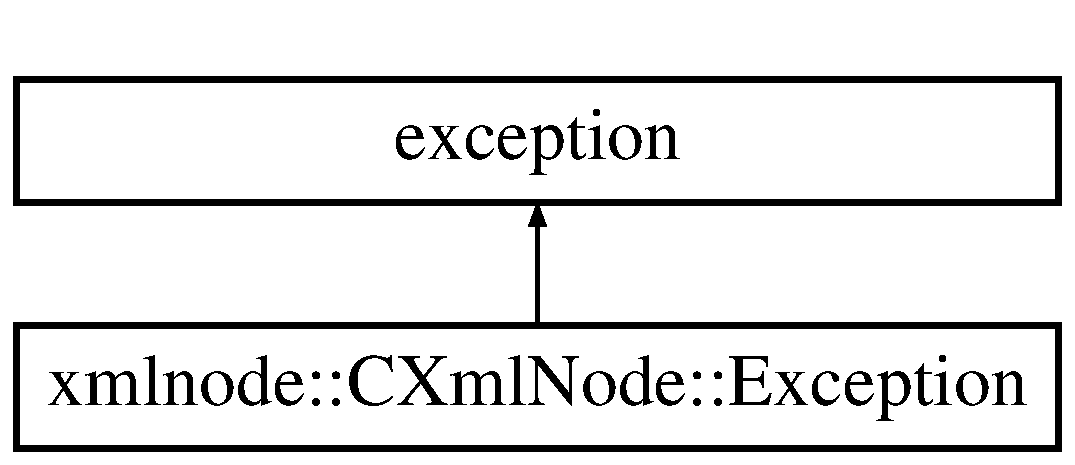
\includegraphics[height=2.000000cm]{classxmlnode_1_1_c_xml_node_1_1_exception}
\end{center}
\end{figure}
\subsection*{Public Types}
\begin{DoxyCompactItemize}
\item 
enum \hyperlink{classxmlnode_1_1_c_xml_node_1_1_exception_abdbe07531ef4b19192f1fa2f819ed75f}{Types} \{ \\*
\hyperlink{classxmlnode_1_1_c_xml_node_1_1_exception_abdbe07531ef4b19192f1fa2f819ed75fa22036006e7862ed7f6fc42091f6a3bc8}{None}, 
\hyperlink{classxmlnode_1_1_c_xml_node_1_1_exception_abdbe07531ef4b19192f1fa2f819ed75fa725fdfe67e4fbd5539133a341a5e0a6e}{Unable\+To\+Open}, 
\hyperlink{classxmlnode_1_1_c_xml_node_1_1_exception_abdbe07531ef4b19192f1fa2f819ed75fab4da3fb6cf56910a8302ddb34b697295}{Unable\+To\+Write}, 
\hyperlink{classxmlnode_1_1_c_xml_node_1_1_exception_abdbe07531ef4b19192f1fa2f819ed75fa34828bed7772bc0588f97192c03ea4ad}{Unable\+To\+Create}, 
\\*
\hyperlink{classxmlnode_1_1_c_xml_node_1_1_exception_abdbe07531ef4b19192f1fa2f819ed75fa5e03a8ddc6c8873e07c6a34dc1d7a0e0}{No\+Root}
 \}
\begin{DoxyCompactList}\small\item\em \hyperlink{classxmlnode_1_1_c_xml_node_1_1_exception}{Exception} types. \end{DoxyCompactList}\end{DoxyCompactItemize}
\subsection*{Public Member Functions}
\begin{DoxyCompactItemize}
\item 
\hypertarget{classxmlnode_1_1_c_xml_node_1_1_exception_ad3078912e0a640db79884170176cb0a8}{\hyperlink{classxmlnode_1_1_c_xml_node_1_1_exception_ad3078912e0a640db79884170176cb0a8}{Exception} ()}\label{classxmlnode_1_1_c_xml_node_1_1_exception_ad3078912e0a640db79884170176cb0a8}

\begin{DoxyCompactList}\small\item\em Default Constructor. \end{DoxyCompactList}\item 
\hyperlink{classxmlnode_1_1_c_xml_node_1_1_exception_aaefc2a485cf66513101ac27c2389c819}{Exception} (const \hyperlink{classxmlnode_1_1_c_xml_node_1_1_exception}{Exception} \&other)
\begin{DoxyCompactList}\small\item\em Copy Constructor. \end{DoxyCompactList}\item 
\hyperlink{classxmlnode_1_1_c_xml_node_1_1_exception}{Exception} \& \hyperlink{classxmlnode_1_1_c_xml_node_1_1_exception_a40c0f5e49e54cd97c4643c71fbc34014}{operator=} (const \hyperlink{classxmlnode_1_1_c_xml_node_1_1_exception}{Exception} \&other)
\begin{DoxyCompactList}\small\item\em Assignment operator. \end{DoxyCompactList}\item 
\hyperlink{classxmlnode_1_1_c_xml_node_1_1_exception_ad660bb87054a9483c0933efbaddfaa55}{Exception} (\hyperlink{classxmlnode_1_1_c_xml_node_1_1_exception_abdbe07531ef4b19192f1fa2f819ed75f}{Types} type, const std\+::wstring \&msg)
\begin{DoxyCompactList}\small\item\em Constructor. \end{DoxyCompactList}\item 
\hypertarget{classxmlnode_1_1_c_xml_node_1_1_exception_ae22ca483e7821c057dec85f06a5e4d32}{virtual \hyperlink{classxmlnode_1_1_c_xml_node_1_1_exception_ae22ca483e7821c057dec85f06a5e4d32}{$\sim$\+Exception} ()}\label{classxmlnode_1_1_c_xml_node_1_1_exception_ae22ca483e7821c057dec85f06a5e4d32}

\begin{DoxyCompactList}\small\item\em Destructor. \end{DoxyCompactList}\item 
virtual const char $\ast$ \hyperlink{classxmlnode_1_1_c_xml_node_1_1_exception_a8313d9c1ddeaa684efc9b1be812ad39b}{what} () const   throw ()
\begin{DoxyCompactList}\small\item\em \hyperlink{classxmlnode_1_1_c_xml_node_1_1_exception}{Exception} message. \end{DoxyCompactList}\item 
std\+::wstring \hyperlink{classxmlnode_1_1_c_xml_node_1_1_exception_a29271ad0ec50958663200f60aaae97b2}{Message} ()
\begin{DoxyCompactList}\small\item\em \hyperlink{classxmlnode_1_1_c_xml_node_1_1_exception}{Exception} message. \end{DoxyCompactList}\item 
\hyperlink{classxmlnode_1_1_c_xml_node_1_1_exception_abdbe07531ef4b19192f1fa2f819ed75f}{Types} \hyperlink{classxmlnode_1_1_c_xml_node_1_1_exception_a872eb6da8739faf5424baf6515b43793}{Type} ()
\begin{DoxyCompactList}\small\item\em \hyperlink{classxmlnode_1_1_c_xml_node_1_1_exception}{Exception} type. \end{DoxyCompactList}\end{DoxyCompactItemize}


\subsection{Detailed Description}
Exceptions for \hyperlink{classxmlnode_1_1_c_xml_node}{C\+Xml\+Node}. 

\subsection{Member Enumeration Documentation}
\hypertarget{classxmlnode_1_1_c_xml_node_1_1_exception_abdbe07531ef4b19192f1fa2f819ed75f}{\index{xmlnode\+::\+C\+Xml\+Node\+::\+Exception@{xmlnode\+::\+C\+Xml\+Node\+::\+Exception}!Types@{Types}}
\index{Types@{Types}!xmlnode\+::\+C\+Xml\+Node\+::\+Exception@{xmlnode\+::\+C\+Xml\+Node\+::\+Exception}}
\subsubsection[{Types}]{\setlength{\rightskip}{0pt plus 5cm}enum {\bf xmlnode\+::\+C\+Xml\+Node\+::\+Exception\+::\+Types}}}\label{classxmlnode_1_1_c_xml_node_1_1_exception_abdbe07531ef4b19192f1fa2f819ed75f}


\hyperlink{classxmlnode_1_1_c_xml_node_1_1_exception}{Exception} types. 

\begin{Desc}
\item[Enumerator]\par
\begin{description}
\index{None@{None}!xmlnode\+::\+C\+Xml\+Node\+::\+Exception@{xmlnode\+::\+C\+Xml\+Node\+::\+Exception}}\index{xmlnode\+::\+C\+Xml\+Node\+::\+Exception@{xmlnode\+::\+C\+Xml\+Node\+::\+Exception}!None@{None}}\item[{\em 
\hypertarget{classxmlnode_1_1_c_xml_node_1_1_exception_abdbe07531ef4b19192f1fa2f819ed75fa22036006e7862ed7f6fc42091f6a3bc8}{None}\label{classxmlnode_1_1_c_xml_node_1_1_exception_abdbe07531ef4b19192f1fa2f819ed75fa22036006e7862ed7f6fc42091f6a3bc8}
}]No exception type indicated. \index{Unable\+To\+Open@{Unable\+To\+Open}!xmlnode\+::\+C\+Xml\+Node\+::\+Exception@{xmlnode\+::\+C\+Xml\+Node\+::\+Exception}}\index{xmlnode\+::\+C\+Xml\+Node\+::\+Exception@{xmlnode\+::\+C\+Xml\+Node\+::\+Exception}!Unable\+To\+Open@{Unable\+To\+Open}}\item[{\em 
\hypertarget{classxmlnode_1_1_c_xml_node_1_1_exception_abdbe07531ef4b19192f1fa2f819ed75fa725fdfe67e4fbd5539133a341a5e0a6e}{Unable\+To\+Open}\label{classxmlnode_1_1_c_xml_node_1_1_exception_abdbe07531ef4b19192f1fa2f819ed75fa725fdfe67e4fbd5539133a341a5e0a6e}
}]Unable to open file to read. \index{Unable\+To\+Write@{Unable\+To\+Write}!xmlnode\+::\+C\+Xml\+Node\+::\+Exception@{xmlnode\+::\+C\+Xml\+Node\+::\+Exception}}\index{xmlnode\+::\+C\+Xml\+Node\+::\+Exception@{xmlnode\+::\+C\+Xml\+Node\+::\+Exception}!Unable\+To\+Write@{Unable\+To\+Write}}\item[{\em 
\hypertarget{classxmlnode_1_1_c_xml_node_1_1_exception_abdbe07531ef4b19192f1fa2f819ed75fab4da3fb6cf56910a8302ddb34b697295}{Unable\+To\+Write}\label{classxmlnode_1_1_c_xml_node_1_1_exception_abdbe07531ef4b19192f1fa2f819ed75fab4da3fb6cf56910a8302ddb34b697295}
}]Unable to open file to write. \index{Unable\+To\+Create@{Unable\+To\+Create}!xmlnode\+::\+C\+Xml\+Node\+::\+Exception@{xmlnode\+::\+C\+Xml\+Node\+::\+Exception}}\index{xmlnode\+::\+C\+Xml\+Node\+::\+Exception@{xmlnode\+::\+C\+Xml\+Node\+::\+Exception}!Unable\+To\+Create@{Unable\+To\+Create}}\item[{\em 
\hypertarget{classxmlnode_1_1_c_xml_node_1_1_exception_abdbe07531ef4b19192f1fa2f819ed75fa34828bed7772bc0588f97192c03ea4ad}{Unable\+To\+Create}\label{classxmlnode_1_1_c_xml_node_1_1_exception_abdbe07531ef4b19192f1fa2f819ed75fa34828bed7772bc0588f97192c03ea4ad}
}]Unable to create X\+M\+L document. \index{No\+Root@{No\+Root}!xmlnode\+::\+C\+Xml\+Node\+::\+Exception@{xmlnode\+::\+C\+Xml\+Node\+::\+Exception}}\index{xmlnode\+::\+C\+Xml\+Node\+::\+Exception@{xmlnode\+::\+C\+Xml\+Node\+::\+Exception}!No\+Root@{No\+Root}}\item[{\em 
\hypertarget{classxmlnode_1_1_c_xml_node_1_1_exception_abdbe07531ef4b19192f1fa2f819ed75fa5e03a8ddc6c8873e07c6a34dc1d7a0e0}{No\+Root}\label{classxmlnode_1_1_c_xml_node_1_1_exception_abdbe07531ef4b19192f1fa2f819ed75fa5e03a8ddc6c8873e07c6a34dc1d7a0e0}
}]Not X\+M\+L document root node. \end{description}
\end{Desc}


\subsection{Constructor \& Destructor Documentation}
\hypertarget{classxmlnode_1_1_c_xml_node_1_1_exception_aaefc2a485cf66513101ac27c2389c819}{\index{xmlnode\+::\+C\+Xml\+Node\+::\+Exception@{xmlnode\+::\+C\+Xml\+Node\+::\+Exception}!Exception@{Exception}}
\index{Exception@{Exception}!xmlnode\+::\+C\+Xml\+Node\+::\+Exception@{xmlnode\+::\+C\+Xml\+Node\+::\+Exception}}
\subsubsection[{Exception}]{\setlength{\rightskip}{0pt plus 5cm}xmlnode\+::\+C\+Xml\+Node\+::\+Exception\+::\+Exception (
\begin{DoxyParamCaption}
\item[{const {\bf Exception} \&}]{other}
\end{DoxyParamCaption}
)\hspace{0.3cm}{\ttfamily [inline]}}}\label{classxmlnode_1_1_c_xml_node_1_1_exception_aaefc2a485cf66513101ac27c2389c819}


Copy Constructor. 


\begin{DoxyParams}{Parameters}
{\em other} & Object to copy \\
\hline
\end{DoxyParams}
\hypertarget{classxmlnode_1_1_c_xml_node_1_1_exception_ad660bb87054a9483c0933efbaddfaa55}{\index{xmlnode\+::\+C\+Xml\+Node\+::\+Exception@{xmlnode\+::\+C\+Xml\+Node\+::\+Exception}!Exception@{Exception}}
\index{Exception@{Exception}!xmlnode\+::\+C\+Xml\+Node\+::\+Exception@{xmlnode\+::\+C\+Xml\+Node\+::\+Exception}}
\subsubsection[{Exception}]{\setlength{\rightskip}{0pt plus 5cm}xmlnode\+::\+C\+Xml\+Node\+::\+Exception\+::\+Exception (
\begin{DoxyParamCaption}
\item[{{\bf Types}}]{type, }
\item[{const std\+::wstring \&}]{msg}
\end{DoxyParamCaption}
)\hspace{0.3cm}{\ttfamily [inline]}}}\label{classxmlnode_1_1_c_xml_node_1_1_exception_ad660bb87054a9483c0933efbaddfaa55}


Constructor. 


\begin{DoxyParams}{Parameters}
{\em type} & \hyperlink{classxmlnode_1_1_c_xml_node_1_1_exception}{Exception} type \\
\hline
{\em msg} & Message associated with exception \\
\hline
\end{DoxyParams}


\subsection{Member Function Documentation}
\hypertarget{classxmlnode_1_1_c_xml_node_1_1_exception_a29271ad0ec50958663200f60aaae97b2}{\index{xmlnode\+::\+C\+Xml\+Node\+::\+Exception@{xmlnode\+::\+C\+Xml\+Node\+::\+Exception}!Message@{Message}}
\index{Message@{Message}!xmlnode\+::\+C\+Xml\+Node\+::\+Exception@{xmlnode\+::\+C\+Xml\+Node\+::\+Exception}}
\subsubsection[{Message}]{\setlength{\rightskip}{0pt plus 5cm}std\+::wstring xmlnode\+::\+C\+Xml\+Node\+::\+Exception\+::\+Message (
\begin{DoxyParamCaption}
{}
\end{DoxyParamCaption}
)\hspace{0.3cm}{\ttfamily [inline]}}}\label{classxmlnode_1_1_c_xml_node_1_1_exception_a29271ad0ec50958663200f60aaae97b2}


\hyperlink{classxmlnode_1_1_c_xml_node_1_1_exception}{Exception} message. 

\begin{DoxyReturn}{Returns}
\hyperlink{classxmlnode_1_1_c_xml_node_1_1_exception}{Exception} message 
\end{DoxyReturn}
\hypertarget{classxmlnode_1_1_c_xml_node_1_1_exception_a40c0f5e49e54cd97c4643c71fbc34014}{\index{xmlnode\+::\+C\+Xml\+Node\+::\+Exception@{xmlnode\+::\+C\+Xml\+Node\+::\+Exception}!operator=@{operator=}}
\index{operator=@{operator=}!xmlnode\+::\+C\+Xml\+Node\+::\+Exception@{xmlnode\+::\+C\+Xml\+Node\+::\+Exception}}
\subsubsection[{operator=}]{\setlength{\rightskip}{0pt plus 5cm}{\bf Exception}\& xmlnode\+::\+C\+Xml\+Node\+::\+Exception\+::operator= (
\begin{DoxyParamCaption}
\item[{const {\bf Exception} \&}]{other}
\end{DoxyParamCaption}
)\hspace{0.3cm}{\ttfamily [inline]}}}\label{classxmlnode_1_1_c_xml_node_1_1_exception_a40c0f5e49e54cd97c4643c71fbc34014}


Assignment operator. 


\begin{DoxyParams}{Parameters}
{\em other} & Object to copy \\
\hline
\end{DoxyParams}
\begin{DoxyReturn}{Returns}
Reference to this object 
\end{DoxyReturn}
\hypertarget{classxmlnode_1_1_c_xml_node_1_1_exception_a872eb6da8739faf5424baf6515b43793}{\index{xmlnode\+::\+C\+Xml\+Node\+::\+Exception@{xmlnode\+::\+C\+Xml\+Node\+::\+Exception}!Type@{Type}}
\index{Type@{Type}!xmlnode\+::\+C\+Xml\+Node\+::\+Exception@{xmlnode\+::\+C\+Xml\+Node\+::\+Exception}}
\subsubsection[{Type}]{\setlength{\rightskip}{0pt plus 5cm}{\bf Types} xmlnode\+::\+C\+Xml\+Node\+::\+Exception\+::\+Type (
\begin{DoxyParamCaption}
{}
\end{DoxyParamCaption}
)\hspace{0.3cm}{\ttfamily [inline]}}}\label{classxmlnode_1_1_c_xml_node_1_1_exception_a872eb6da8739faf5424baf6515b43793}


\hyperlink{classxmlnode_1_1_c_xml_node_1_1_exception}{Exception} type. 

\begin{DoxyReturn}{Returns}
\hyperlink{classxmlnode_1_1_c_xml_node_1_1_exception}{Exception} type of type \hyperlink{classxmlnode_1_1_c_xml_node_1_1_exception_abdbe07531ef4b19192f1fa2f819ed75f}{C\+Xml\+Node\+::\+Exception\+::\+Types} 
\end{DoxyReturn}
\hypertarget{classxmlnode_1_1_c_xml_node_1_1_exception_a8313d9c1ddeaa684efc9b1be812ad39b}{\index{xmlnode\+::\+C\+Xml\+Node\+::\+Exception@{xmlnode\+::\+C\+Xml\+Node\+::\+Exception}!what@{what}}
\index{what@{what}!xmlnode\+::\+C\+Xml\+Node\+::\+Exception@{xmlnode\+::\+C\+Xml\+Node\+::\+Exception}}
\subsubsection[{what}]{\setlength{\rightskip}{0pt plus 5cm}virtual const char$\ast$ xmlnode\+::\+C\+Xml\+Node\+::\+Exception\+::what (
\begin{DoxyParamCaption}
{}
\end{DoxyParamCaption}
) const throw  ) \hspace{0.3cm}{\ttfamily [inline]}, {\ttfamily [virtual]}}}\label{classxmlnode_1_1_c_xml_node_1_1_exception_a8313d9c1ddeaa684efc9b1be812ad39b}


\hyperlink{classxmlnode_1_1_c_xml_node_1_1_exception}{Exception} message. 

More verbose exception messages are provided in Unicode as they should be by the \hyperlink{classxmlnode_1_1_c_xml_node_1_1_exception_a29271ad0ec50958663200f60aaae97b2}{Message()} function. \begin{DoxyReturn}{Returns}
\char`\"{}\+C\+Xml\+Node exception\char`\"{} 
\end{DoxyReturn}


The documentation for this class was generated from the following file\+:\begin{DoxyCompactItemize}
\item 
\hyperlink{_xml_node_8h}{Xml\+Node.\+h}\end{DoxyCompactItemize}

\hypertarget{classxmlnode_1_1_c_xml_node_1_1_iterator}{\section{xmlnode\+:\+:C\+Xml\+Node\+:\+:Iterator Class Reference}
\label{classxmlnode_1_1_c_xml_node_1_1_iterator}\index{xmlnode\+::\+C\+Xml\+Node\+::\+Iterator@{xmlnode\+::\+C\+Xml\+Node\+::\+Iterator}}
}


Support for iterating over the children of a node.  




{\ttfamily \#include $<$Xml\+Node.\+h$>$}

\subsection*{Public Member Functions}
\begin{DoxyCompactItemize}
\item 
bool \hyperlink{classxmlnode_1_1_c_xml_node_1_1_iterator_a9907b45ce49352e0d5ffafa7f2c4a520}{operator!=} (const \hyperlink{classxmlnode_1_1_c_xml_node_1_1_iterator}{Iterator} \&other) const 
\begin{DoxyCompactList}\small\item\em Test to see if two iterator are at the same location. \end{DoxyCompactList}\item 
std\+::shared\+\_\+ptr$<$ \hyperlink{classxmlnode_1_1_c_xml_node}{C\+Xml\+Node} $>$ \hyperlink{classxmlnode_1_1_c_xml_node_1_1_iterator_a6d255a513c60c7de55a01c5eb626bf6d}{operator$\ast$} ()
\begin{DoxyCompactList}\small\item\em Operation $\ast$ for the iterator. \end{DoxyCompactList}\item 
const \hyperlink{classxmlnode_1_1_c_xml_node_1_1_iterator}{Iterator} \& \hyperlink{classxmlnode_1_1_c_xml_node_1_1_iterator_aefa7392f7c198dcf907d8458fbf0db1a}{operator++} ()
\begin{DoxyCompactList}\small\item\em Advance to the next item in the collection. \end{DoxyCompactList}\end{DoxyCompactItemize}
\subsection*{Friends}
\begin{DoxyCompactItemize}
\item 
\hypertarget{classxmlnode_1_1_c_xml_node_1_1_iterator_a770307dc9d4e2e7005bcf200bae3066a}{class {\bfseries C\+Xml\+Node}}\label{classxmlnode_1_1_c_xml_node_1_1_iterator_a770307dc9d4e2e7005bcf200bae3066a}

\end{DoxyCompactItemize}


\subsection{Detailed Description}
Support for iterating over the children of a node. 

\subsection{Member Function Documentation}
\hypertarget{classxmlnode_1_1_c_xml_node_1_1_iterator_a9907b45ce49352e0d5ffafa7f2c4a520}{\index{xmlnode\+::\+C\+Xml\+Node\+::\+Iterator@{xmlnode\+::\+C\+Xml\+Node\+::\+Iterator}!operator"!=@{operator"!=}}
\index{operator"!=@{operator"!=}!xmlnode\+::\+C\+Xml\+Node\+::\+Iterator@{xmlnode\+::\+C\+Xml\+Node\+::\+Iterator}}
\subsubsection[{operator"!=}]{\setlength{\rightskip}{0pt plus 5cm}bool xmlnode\+::\+C\+Xml\+Node\+::\+Iterator\+::operator!= (
\begin{DoxyParamCaption}
\item[{const {\bf Iterator} \&}]{other}
\end{DoxyParamCaption}
) const\hspace{0.3cm}{\ttfamily [inline]}}}\label{classxmlnode_1_1_c_xml_node_1_1_iterator_a9907b45ce49352e0d5ffafa7f2c4a520}


Test to see if two iterator are at the same location. 


\begin{DoxyParams}{Parameters}
{\em other} & The other object we are testing against \\
\hline
\end{DoxyParams}
\begin{DoxyReturn}{Returns}
true if they are equal. 
\end{DoxyReturn}
\hypertarget{classxmlnode_1_1_c_xml_node_1_1_iterator_a6d255a513c60c7de55a01c5eb626bf6d}{\index{xmlnode\+::\+C\+Xml\+Node\+::\+Iterator@{xmlnode\+::\+C\+Xml\+Node\+::\+Iterator}!operator$\ast$@{operator$\ast$}}
\index{operator$\ast$@{operator$\ast$}!xmlnode\+::\+C\+Xml\+Node\+::\+Iterator@{xmlnode\+::\+C\+Xml\+Node\+::\+Iterator}}
\subsubsection[{operator$\ast$}]{\setlength{\rightskip}{0pt plus 5cm}std\+::shared\+\_\+ptr$<$ {\bf C\+Xml\+Node} $>$ C\+Xml\+Node\+::\+Iterator\+::operator$\ast$ (
\begin{DoxyParamCaption}
{}
\end{DoxyParamCaption}
)}}\label{classxmlnode_1_1_c_xml_node_1_1_iterator_a6d255a513c60c7de55a01c5eb626bf6d}


Operation $\ast$ for the iterator. 

Indiates the child that is the current iterator reference.

\begin{DoxyReturn}{Returns}
Pointer to child node. 
\end{DoxyReturn}
\hypertarget{classxmlnode_1_1_c_xml_node_1_1_iterator_aefa7392f7c198dcf907d8458fbf0db1a}{\index{xmlnode\+::\+C\+Xml\+Node\+::\+Iterator@{xmlnode\+::\+C\+Xml\+Node\+::\+Iterator}!operator++@{operator++}}
\index{operator++@{operator++}!xmlnode\+::\+C\+Xml\+Node\+::\+Iterator@{xmlnode\+::\+C\+Xml\+Node\+::\+Iterator}}
\subsubsection[{operator++}]{\setlength{\rightskip}{0pt plus 5cm}const {\bf Iterator}\& xmlnode\+::\+C\+Xml\+Node\+::\+Iterator\+::operator++ (
\begin{DoxyParamCaption}
{}
\end{DoxyParamCaption}
)\hspace{0.3cm}{\ttfamily [inline]}}}\label{classxmlnode_1_1_c_xml_node_1_1_iterator_aefa7392f7c198dcf907d8458fbf0db1a}


Advance to the next item in the collection. 

\begin{DoxyReturn}{Returns}
Reference to this iterator. 
\end{DoxyReturn}


The documentation for this class was generated from the following files\+:\begin{DoxyCompactItemize}
\item 
\hyperlink{_xml_node_8h}{Xml\+Node.\+h}\item 
\hyperlink{_xml_node_8cpp}{Xml\+Node.\+cpp}\end{DoxyCompactItemize}

\hypertarget{class_c_anim_channel_1_1_keyframe}{\section{C\+Anim\+Channel\+:\+:Keyframe Class Reference}
\label{class_c_anim_channel_1_1_keyframe}\index{C\+Anim\+Channel\+::\+Keyframe@{C\+Anim\+Channel\+::\+Keyframe}}
}


Class that represents a keyframe.  




{\ttfamily \#include $<$Anim\+Channel.\+h$>$}

Inheritance diagram for C\+Anim\+Channel\+:\+:Keyframe\+:\begin{figure}[H]
\begin{center}
\leavevmode
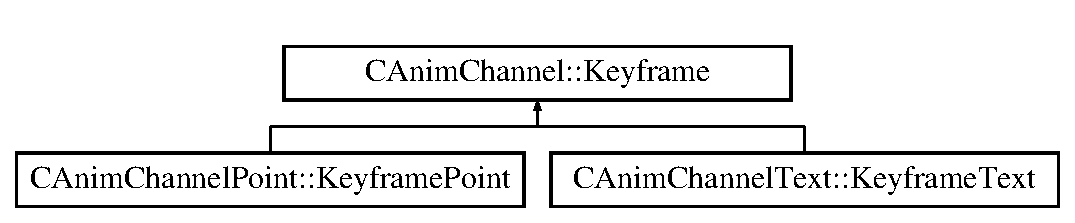
\includegraphics[height=2.000000cm]{class_c_anim_channel_1_1_keyframe}
\end{center}
\end{figure}
\subsection*{Public Member Functions}
\begin{DoxyCompactItemize}
\item 
\hypertarget{class_c_anim_channel_1_1_keyframe_a88096d3eecc2aa502bae62906107c8c1}{\hyperlink{class_c_anim_channel_1_1_keyframe_a88096d3eecc2aa502bae62906107c8c1}{Keyframe} ()=delete}\label{class_c_anim_channel_1_1_keyframe_a88096d3eecc2aa502bae62906107c8c1}

\begin{DoxyCompactList}\small\item\em Default constructor disabled. \end{DoxyCompactList}\item 
\hypertarget{class_c_anim_channel_1_1_keyframe_a3f1c6e4c4eba22d6b8bdd6aa971d0200}{\hyperlink{class_c_anim_channel_1_1_keyframe_a3f1c6e4c4eba22d6b8bdd6aa971d0200}{Keyframe} (const \hyperlink{class_c_anim_channel_1_1_keyframe}{Keyframe} \&)=delete}\label{class_c_anim_channel_1_1_keyframe_a3f1c6e4c4eba22d6b8bdd6aa971d0200}

\begin{DoxyCompactList}\small\item\em Copy constructor disabled. \end{DoxyCompactList}\item 
\hypertarget{class_c_anim_channel_1_1_keyframe_a0b5fe25a49eba43386aa4e9e91ad3b54}{void \hyperlink{class_c_anim_channel_1_1_keyframe_a0b5fe25a49eba43386aa4e9e91ad3b54}{operator=} (const \hyperlink{class_c_anim_channel_1_1_keyframe}{Keyframe} \&)=delete}\label{class_c_anim_channel_1_1_keyframe_a0b5fe25a49eba43386aa4e9e91ad3b54}

\begin{DoxyCompactList}\small\item\em Assignment operator disabled. \end{DoxyCompactList}\item 
int \hyperlink{class_c_anim_channel_1_1_keyframe_ab772a5915170d21d88e9259dbed24191}{Get\+Frame} () const 
\begin{DoxyCompactList}\small\item\em Get the frame for this keyframe. \end{DoxyCompactList}\item 
void \hyperlink{class_c_anim_channel_1_1_keyframe_a19e0ffcf6eab8a2c9eef7cd35f0ca8d7}{Set\+Frame} (int f)
\begin{DoxyCompactList}\small\item\em Set the frame for this keyframe. \end{DoxyCompactList}\item 
\hypertarget{class_c_anim_channel_1_1_keyframe_ab299b5d67b1a6314421dd0d718f15493}{virtual void \hyperlink{class_c_anim_channel_1_1_keyframe_ab299b5d67b1a6314421dd0d718f15493}{Use\+As1} ()=0}\label{class_c_anim_channel_1_1_keyframe_ab299b5d67b1a6314421dd0d718f15493}

\begin{DoxyCompactList}\small\item\em Indicates this keyframe is used as Keyframe1. \end{DoxyCompactList}\item 
\hypertarget{class_c_anim_channel_1_1_keyframe_acee82565971cf385abbc94c4fd29c6a5}{virtual void \hyperlink{class_c_anim_channel_1_1_keyframe_acee82565971cf385abbc94c4fd29c6a5}{Use\+As2} ()=0}\label{class_c_anim_channel_1_1_keyframe_acee82565971cf385abbc94c4fd29c6a5}

\begin{DoxyCompactList}\small\item\em Indicates this keyframe is used as Keyframe2. \end{DoxyCompactList}\item 
\hypertarget{class_c_anim_channel_1_1_keyframe_a70a183c3caabf9b820d41cae4d5fa5ae}{virtual void \hyperlink{class_c_anim_channel_1_1_keyframe_a70a183c3caabf9b820d41cae4d5fa5ae}{Use\+Only} ()=0}\label{class_c_anim_channel_1_1_keyframe_a70a183c3caabf9b820d41cae4d5fa5ae}

\begin{DoxyCompactList}\small\item\em Indicates this is the only keyframe. \end{DoxyCompactList}\item 
virtual std\+::shared\+\_\+ptr\\*
$<$ \hyperlink{classxmlnode_1_1_c_xml_node}{xmlnode\+::\+C\+Xml\+Node} $>$ \hyperlink{class_c_anim_channel_1_1_keyframe_a2dbc0b264510a45b9a429f64aa2d8448}{Xml\+Save} (const std\+::shared\+\_\+ptr$<$ \hyperlink{classxmlnode_1_1_c_xml_node}{xmlnode\+::\+C\+Xml\+Node} $>$ \&node)
\begin{DoxyCompactList}\small\item\em Save this keyframe to an X\+M\+L node. \end{DoxyCompactList}\end{DoxyCompactItemize}
\subsection*{Protected Member Functions}
\begin{DoxyCompactItemize}
\item 
\hyperlink{class_c_anim_channel_1_1_keyframe_a123c8c5557957a1202d9987fce83b31e}{Keyframe} (\hyperlink{class_c_anim_channel}{C\+Anim\+Channel} $\ast$channel)
\begin{DoxyCompactList}\small\item\em Constructor. \end{DoxyCompactList}\end{DoxyCompactItemize}
\subsection*{Protected Attributes}
\begin{DoxyCompactItemize}
\item 
\hypertarget{class_c_anim_channel_1_1_keyframe_ae946ed89ac4a6b4ecb6cefd5a64777a7}{int \hyperlink{class_c_anim_channel_1_1_keyframe_ae946ed89ac4a6b4ecb6cefd5a64777a7}{m\+Frame}}\label{class_c_anim_channel_1_1_keyframe_ae946ed89ac4a6b4ecb6cefd5a64777a7}

\begin{DoxyCompactList}\small\item\em The frame number for the keyframe. \end{DoxyCompactList}\end{DoxyCompactItemize}


\subsection{Detailed Description}
Class that represents a keyframe. 

\subsection{Constructor \& Destructor Documentation}
\hypertarget{class_c_anim_channel_1_1_keyframe_a123c8c5557957a1202d9987fce83b31e}{\index{C\+Anim\+Channel\+::\+Keyframe@{C\+Anim\+Channel\+::\+Keyframe}!Keyframe@{Keyframe}}
\index{Keyframe@{Keyframe}!C\+Anim\+Channel\+::\+Keyframe@{C\+Anim\+Channel\+::\+Keyframe}}
\subsubsection[{Keyframe}]{\setlength{\rightskip}{0pt plus 5cm}C\+Anim\+Channel\+::\+Keyframe\+::\+Keyframe (
\begin{DoxyParamCaption}
\item[{{\bf C\+Anim\+Channel} $\ast$}]{channel}
\end{DoxyParamCaption}
)\hspace{0.3cm}{\ttfamily [inline]}, {\ttfamily [protected]}}}\label{class_c_anim_channel_1_1_keyframe_a123c8c5557957a1202d9987fce83b31e}


Constructor. 


\begin{DoxyParams}{Parameters}
{\em channel} & Channel we are associated with \\
\hline
\end{DoxyParams}


\subsection{Member Function Documentation}
\hypertarget{class_c_anim_channel_1_1_keyframe_ab772a5915170d21d88e9259dbed24191}{\index{C\+Anim\+Channel\+::\+Keyframe@{C\+Anim\+Channel\+::\+Keyframe}!Get\+Frame@{Get\+Frame}}
\index{Get\+Frame@{Get\+Frame}!C\+Anim\+Channel\+::\+Keyframe@{C\+Anim\+Channel\+::\+Keyframe}}
\subsubsection[{Get\+Frame}]{\setlength{\rightskip}{0pt plus 5cm}int C\+Anim\+Channel\+::\+Keyframe\+::\+Get\+Frame (
\begin{DoxyParamCaption}
{}
\end{DoxyParamCaption}
) const\hspace{0.3cm}{\ttfamily [inline]}}}\label{class_c_anim_channel_1_1_keyframe_ab772a5915170d21d88e9259dbed24191}


Get the frame for this keyframe. 

\begin{DoxyReturn}{Returns}
The keyframe frame number 
\end{DoxyReturn}
\hypertarget{class_c_anim_channel_1_1_keyframe_a19e0ffcf6eab8a2c9eef7cd35f0ca8d7}{\index{C\+Anim\+Channel\+::\+Keyframe@{C\+Anim\+Channel\+::\+Keyframe}!Set\+Frame@{Set\+Frame}}
\index{Set\+Frame@{Set\+Frame}!C\+Anim\+Channel\+::\+Keyframe@{C\+Anim\+Channel\+::\+Keyframe}}
\subsubsection[{Set\+Frame}]{\setlength{\rightskip}{0pt plus 5cm}void C\+Anim\+Channel\+::\+Keyframe\+::\+Set\+Frame (
\begin{DoxyParamCaption}
\item[{int}]{f}
\end{DoxyParamCaption}
)\hspace{0.3cm}{\ttfamily [inline]}}}\label{class_c_anim_channel_1_1_keyframe_a19e0ffcf6eab8a2c9eef7cd35f0ca8d7}


Set the frame for this keyframe. 


\begin{DoxyParams}{Parameters}
{\em f} & The new frame number to set \\
\hline
\end{DoxyParams}
\hypertarget{class_c_anim_channel_1_1_keyframe_a2dbc0b264510a45b9a429f64aa2d8448}{\index{C\+Anim\+Channel\+::\+Keyframe@{C\+Anim\+Channel\+::\+Keyframe}!Xml\+Save@{Xml\+Save}}
\index{Xml\+Save@{Xml\+Save}!C\+Anim\+Channel\+::\+Keyframe@{C\+Anim\+Channel\+::\+Keyframe}}
\subsubsection[{Xml\+Save}]{\setlength{\rightskip}{0pt plus 5cm}std\+::shared\+\_\+ptr$<$ {\bf xmlnode\+::\+C\+Xml\+Node} $>$ C\+Anim\+Channel\+::\+Keyframe\+::\+Xml\+Save (
\begin{DoxyParamCaption}
\item[{const std\+::shared\+\_\+ptr$<$ {\bf xmlnode\+::\+C\+Xml\+Node} $>$ \&}]{node}
\end{DoxyParamCaption}
)\hspace{0.3cm}{\ttfamily [virtual]}}}\label{class_c_anim_channel_1_1_keyframe_a2dbc0b264510a45b9a429f64aa2d8448}


Save this keyframe to an X\+M\+L node. 


\begin{DoxyParams}{Parameters}
{\em node} & The node we are going to be a child of \\
\hline
\end{DoxyParams}
\begin{DoxyReturn}{Returns}
Allocated X\+M\+L node 
\end{DoxyReturn}


Reimplemented in \hyperlink{class_c_anim_channel_text_1_1_keyframe_text_a502cf5d31023f7d1272c4e1a85f94e31}{C\+Anim\+Channel\+Text\+::\+Keyframe\+Text}, and \hyperlink{class_c_anim_channel_point_1_1_keyframe_point_a531900a8e7e5e9d579d92364ff469844}{C\+Anim\+Channel\+Point\+::\+Keyframe\+Point}.



The documentation for this class was generated from the following files\+:\begin{DoxyCompactItemize}
\item 
\hyperlink{_anim_channel_8h}{Anim\+Channel.\+h}\item 
\hyperlink{_anim_channel_8cpp}{Anim\+Channel.\+cpp}\end{DoxyCompactItemize}

\hypertarget{class_c_anim_channel_angle_1_1_keyframe_angle}{\section{C\+Anim\+Channel\+Angle\+:\+:Keyframe\+Angle Class Reference}
\label{class_c_anim_channel_angle_1_1_keyframe_angle}\index{C\+Anim\+Channel\+Angle\+::\+Keyframe\+Angle@{C\+Anim\+Channel\+Angle\+::\+Keyframe\+Angle}}
}


A keyframe for an angle channel.  




{\ttfamily \#include $<$Anim\+Channel\+Angle.\+h$>$}

Inheritance diagram for C\+Anim\+Channel\+Angle\+:\+:Keyframe\+Angle\+:\begin{figure}[H]
\begin{center}
\leavevmode
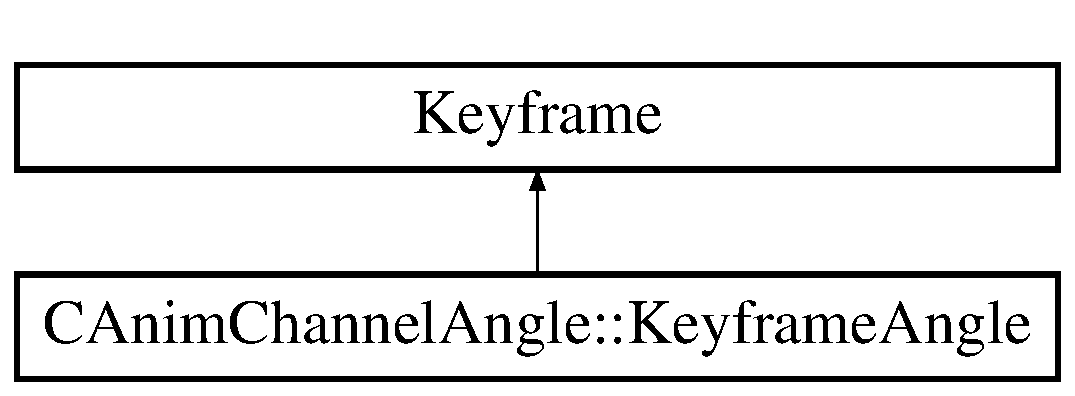
\includegraphics[height=2.000000cm]{class_c_anim_channel_angle_1_1_keyframe_angle}
\end{center}
\end{figure}
\subsection*{Public Member Functions}
\begin{DoxyCompactItemize}
\item 
\hyperlink{class_c_anim_channel_angle_1_1_keyframe_angle_a9b380a2c04fb7b7ff3c63b307308417e}{Keyframe\+Angle} (\hyperlink{class_c_anim_channel_angle}{C\+Anim\+Channel\+Angle} $\ast$channel, double angle)
\begin{DoxyCompactList}\small\item\em Constructor. \end{DoxyCompactList}\item 
\hypertarget{class_c_anim_channel_angle_1_1_keyframe_angle_a25a8c43df01c199a63ee1b31af91b92b}{\hyperlink{class_c_anim_channel_angle_1_1_keyframe_angle_a25a8c43df01c199a63ee1b31af91b92b}{$\sim$\+Keyframe\+Angle} ()}\label{class_c_anim_channel_angle_1_1_keyframe_angle_a25a8c43df01c199a63ee1b31af91b92b}

\begin{DoxyCompactList}\small\item\em Destructor. \end{DoxyCompactList}\item 
\hypertarget{class_c_anim_channel_angle_1_1_keyframe_angle_a5df8c79eb056ae196b44a46c52dfba08}{\hyperlink{class_c_anim_channel_angle_1_1_keyframe_angle_a5df8c79eb056ae196b44a46c52dfba08}{Keyframe\+Angle} ()=delete}\label{class_c_anim_channel_angle_1_1_keyframe_angle_a5df8c79eb056ae196b44a46c52dfba08}

\begin{DoxyCompactList}\small\item\em Default constructor disabled. \end{DoxyCompactList}\item 
\hypertarget{class_c_anim_channel_angle_1_1_keyframe_angle_aca6888d33728e9dd31f63ca3ff37583b}{\hyperlink{class_c_anim_channel_angle_1_1_keyframe_angle_aca6888d33728e9dd31f63ca3ff37583b}{Keyframe\+Angle} (const \hyperlink{class_c_anim_channel_angle_1_1_keyframe_angle}{Keyframe\+Angle} \&)=delete}\label{class_c_anim_channel_angle_1_1_keyframe_angle_aca6888d33728e9dd31f63ca3ff37583b}

\begin{DoxyCompactList}\small\item\em Copy constructor disabled. \end{DoxyCompactList}\item 
\hypertarget{class_c_anim_channel_angle_1_1_keyframe_angle_a2fe8576d29fba09b2b1ae03e3d6df0a0}{void \hyperlink{class_c_anim_channel_angle_1_1_keyframe_angle_a2fe8576d29fba09b2b1ae03e3d6df0a0}{operator=} (const \hyperlink{class_c_anim_channel_angle_1_1_keyframe_angle}{Keyframe\+Angle} \&)=delete}\label{class_c_anim_channel_angle_1_1_keyframe_angle_a2fe8576d29fba09b2b1ae03e3d6df0a0}

\begin{DoxyCompactList}\small\item\em Assignment operator disabled. \end{DoxyCompactList}\item 
double \hyperlink{class_c_anim_channel_angle_1_1_keyframe_angle_a2bcfb0054c78424b3eb4a4b9950d9b9c}{Get\+Angle} ()
\begin{DoxyCompactList}\small\item\em Get the angle at this keyframe. \end{DoxyCompactList}\item 
\hypertarget{class_c_anim_channel_angle_1_1_keyframe_angle_a539433fabd4f3ca88cdac75e087571f7}{virtual void \hyperlink{class_c_anim_channel_angle_1_1_keyframe_angle_a539433fabd4f3ca88cdac75e087571f7}{Use\+As1} () override}\label{class_c_anim_channel_angle_1_1_keyframe_angle_a539433fabd4f3ca88cdac75e087571f7}

\begin{DoxyCompactList}\small\item\em Use this keyframe as keyframe 1. \end{DoxyCompactList}\item 
\hypertarget{class_c_anim_channel_angle_1_1_keyframe_angle_ac11ffb0bf6bb63c4f8bc61f5cfbc90fe}{virtual void \hyperlink{class_c_anim_channel_angle_1_1_keyframe_angle_ac11ffb0bf6bb63c4f8bc61f5cfbc90fe}{Use\+As2} () override}\label{class_c_anim_channel_angle_1_1_keyframe_angle_ac11ffb0bf6bb63c4f8bc61f5cfbc90fe}

\begin{DoxyCompactList}\small\item\em Use this keyframe as keyfraem 2. \end{DoxyCompactList}\item 
\hypertarget{class_c_anim_channel_angle_1_1_keyframe_angle_a75483355e52ab73210c4b6a26d3494b1}{virtual void \hyperlink{class_c_anim_channel_angle_1_1_keyframe_angle_a75483355e52ab73210c4b6a26d3494b1}{Use\+Only} () override}\label{class_c_anim_channel_angle_1_1_keyframe_angle_a75483355e52ab73210c4b6a26d3494b1}

\begin{DoxyCompactList}\small\item\em Use this keyframe as the angle. \end{DoxyCompactList}\item 
virtual std\+::shared\+\_\+ptr\\*
$<$ \hyperlink{classxmlnode_1_1_c_xml_node}{xmlnode\+::\+C\+Xml\+Node} $>$ \hyperlink{class_c_anim_channel_angle_1_1_keyframe_angle_af5d88921f81522bfa70fab8d2a49904b}{Xml\+Save} (const std\+::shared\+\_\+ptr$<$ \hyperlink{classxmlnode_1_1_c_xml_node}{xmlnode\+::\+C\+Xml\+Node} $>$ \&node)
\begin{DoxyCompactList}\small\item\em Save this keyframe to an X\+M\+L node. \end{DoxyCompactList}\end{DoxyCompactItemize}


\subsection{Detailed Description}
A keyframe for an angle channel. 

\subsection{Constructor \& Destructor Documentation}
\hypertarget{class_c_anim_channel_angle_1_1_keyframe_angle_a9b380a2c04fb7b7ff3c63b307308417e}{\index{C\+Anim\+Channel\+Angle\+::\+Keyframe\+Angle@{C\+Anim\+Channel\+Angle\+::\+Keyframe\+Angle}!Keyframe\+Angle@{Keyframe\+Angle}}
\index{Keyframe\+Angle@{Keyframe\+Angle}!C\+Anim\+Channel\+Angle\+::\+Keyframe\+Angle@{C\+Anim\+Channel\+Angle\+::\+Keyframe\+Angle}}
\subsubsection[{Keyframe\+Angle}]{\setlength{\rightskip}{0pt plus 5cm}C\+Anim\+Channel\+Angle\+::\+Keyframe\+Angle\+::\+Keyframe\+Angle (
\begin{DoxyParamCaption}
\item[{{\bf C\+Anim\+Channel\+Angle} $\ast$}]{channel, }
\item[{double}]{angle}
\end{DoxyParamCaption}
)\hspace{0.3cm}{\ttfamily [inline]}}}\label{class_c_anim_channel_angle_1_1_keyframe_angle_a9b380a2c04fb7b7ff3c63b307308417e}


Constructor. 


\begin{DoxyParams}{Parameters}
{\em channel} & The channel we are for \\
\hline
{\em angle} & The angle for the keyframe \\
\hline
\end{DoxyParams}


\subsection{Member Function Documentation}
\hypertarget{class_c_anim_channel_angle_1_1_keyframe_angle_a2bcfb0054c78424b3eb4a4b9950d9b9c}{\index{C\+Anim\+Channel\+Angle\+::\+Keyframe\+Angle@{C\+Anim\+Channel\+Angle\+::\+Keyframe\+Angle}!Get\+Angle@{Get\+Angle}}
\index{Get\+Angle@{Get\+Angle}!C\+Anim\+Channel\+Angle\+::\+Keyframe\+Angle@{C\+Anim\+Channel\+Angle\+::\+Keyframe\+Angle}}
\subsubsection[{Get\+Angle}]{\setlength{\rightskip}{0pt plus 5cm}double C\+Anim\+Channel\+Angle\+::\+Keyframe\+Angle\+::\+Get\+Angle (
\begin{DoxyParamCaption}
{}
\end{DoxyParamCaption}
)\hspace{0.3cm}{\ttfamily [inline]}}}\label{class_c_anim_channel_angle_1_1_keyframe_angle_a2bcfb0054c78424b3eb4a4b9950d9b9c}


Get the angle at this keyframe. 

\begin{DoxyReturn}{Returns}
Angle in radians 
\end{DoxyReturn}
\hypertarget{class_c_anim_channel_angle_1_1_keyframe_angle_af5d88921f81522bfa70fab8d2a49904b}{\index{C\+Anim\+Channel\+Angle\+::\+Keyframe\+Angle@{C\+Anim\+Channel\+Angle\+::\+Keyframe\+Angle}!Xml\+Save@{Xml\+Save}}
\index{Xml\+Save@{Xml\+Save}!C\+Anim\+Channel\+Angle\+::\+Keyframe\+Angle@{C\+Anim\+Channel\+Angle\+::\+Keyframe\+Angle}}
\subsubsection[{Xml\+Save}]{\setlength{\rightskip}{0pt plus 5cm}std\+::shared\+\_\+ptr$<$ {\bf xmlnode\+::\+C\+Xml\+Node} $>$ C\+Anim\+Channel\+Angle\+::\+Keyframe\+Angle\+::\+Xml\+Save (
\begin{DoxyParamCaption}
\item[{const std\+::shared\+\_\+ptr$<$ {\bf xmlnode\+::\+C\+Xml\+Node} $>$ \&}]{node}
\end{DoxyParamCaption}
)\hspace{0.3cm}{\ttfamily [virtual]}}}\label{class_c_anim_channel_angle_1_1_keyframe_angle_af5d88921f81522bfa70fab8d2a49904b}


Save this keyframe to an X\+M\+L node. 


\begin{DoxyParams}{Parameters}
{\em node} & The node we are going to be a child of \\
\hline
\end{DoxyParams}
\begin{DoxyReturn}{Returns}
Allocated X\+M\+L node. 
\end{DoxyReturn}


The documentation for this class was generated from the following files\+:\begin{DoxyCompactItemize}
\item 
\hyperlink{_anim_channel_angle_8h}{Anim\+Channel\+Angle.\+h}\item 
\hyperlink{_anim_channel_angle_8cpp}{Anim\+Channel\+Angle.\+cpp}\end{DoxyCompactItemize}

\hypertarget{class_c_anim_channel_point_1_1_keyframe_point}{\section{C\+Anim\+Channel\+Point\+:\+:Keyframe\+Point Class Reference}
\label{class_c_anim_channel_point_1_1_keyframe_point}\index{C\+Anim\+Channel\+Point\+::\+Keyframe\+Point@{C\+Anim\+Channel\+Point\+::\+Keyframe\+Point}}
}


A keyframe for a point channel.  




{\ttfamily \#include $<$Anim\+Channel\+Point.\+h$>$}

Inheritance diagram for C\+Anim\+Channel\+Point\+:\+:Keyframe\+Point\+:\begin{figure}[H]
\begin{center}
\leavevmode
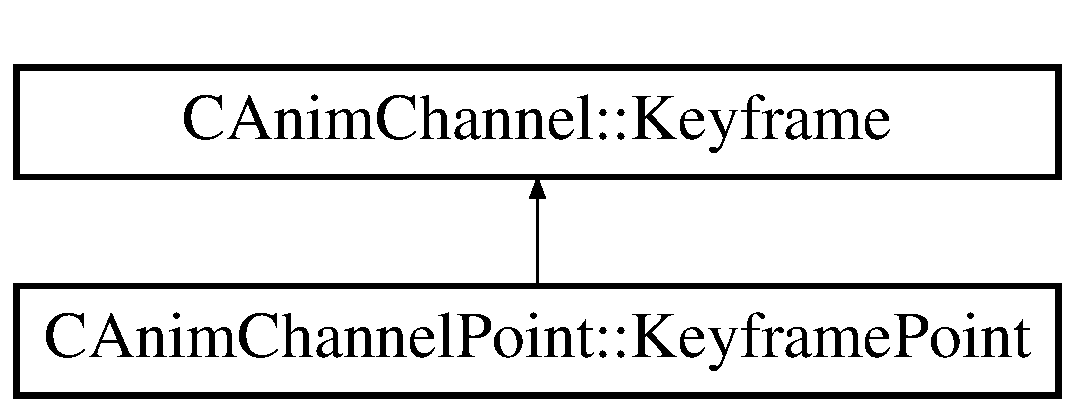
\includegraphics[height=2.000000cm]{class_c_anim_channel_point_1_1_keyframe_point}
\end{center}
\end{figure}
\subsection*{Public Member Functions}
\begin{DoxyCompactItemize}
\item 
\hyperlink{class_c_anim_channel_point_1_1_keyframe_point_af85af782373e964e25ca7238170c927e}{Keyframe\+Point} (\hyperlink{class_c_anim_channel_point}{C\+Anim\+Channel\+Point} $\ast$channel, Gdiplus\+::\+Point point)
\begin{DoxyCompactList}\small\item\em Constructor. \end{DoxyCompactList}\item 
\hypertarget{class_c_anim_channel_point_1_1_keyframe_point_a62d4675ea40bfba7911404dda2ec5065}{\hyperlink{class_c_anim_channel_point_1_1_keyframe_point_a62d4675ea40bfba7911404dda2ec5065}{Keyframe\+Point} ()=delete}\label{class_c_anim_channel_point_1_1_keyframe_point_a62d4675ea40bfba7911404dda2ec5065}

\begin{DoxyCompactList}\small\item\em Default constructor disabled. \end{DoxyCompactList}\item 
\hypertarget{class_c_anim_channel_point_1_1_keyframe_point_abf2e4236b5f8dd0c57cf61dd258bfc6f}{\hyperlink{class_c_anim_channel_point_1_1_keyframe_point_abf2e4236b5f8dd0c57cf61dd258bfc6f}{Keyframe\+Point} (const \hyperlink{class_c_anim_channel_point_1_1_keyframe_point}{Keyframe\+Point} \&)=delete}\label{class_c_anim_channel_point_1_1_keyframe_point_abf2e4236b5f8dd0c57cf61dd258bfc6f}

\begin{DoxyCompactList}\small\item\em Copy constructor disabled. \end{DoxyCompactList}\item 
\hypertarget{class_c_anim_channel_point_1_1_keyframe_point_a7d54b4fb38136049f4d7fea3c12dc5f2}{void \hyperlink{class_c_anim_channel_point_1_1_keyframe_point_a7d54b4fb38136049f4d7fea3c12dc5f2}{operator=} (const \hyperlink{class_c_anim_channel_point_1_1_keyframe_point}{Keyframe\+Point} \&)=delete}\label{class_c_anim_channel_point_1_1_keyframe_point_a7d54b4fb38136049f4d7fea3c12dc5f2}

\begin{DoxyCompactList}\small\item\em Assignment operator disabled. \end{DoxyCompactList}\item 
Gdiplus\+::\+Point \hyperlink{class_c_anim_channel_point_1_1_keyframe_point_a77739c3169abf796b3fb8b20b6cbf222}{Get\+Point} ()
\begin{DoxyCompactList}\small\item\em The keyframe point. \end{DoxyCompactList}\item 
\hypertarget{class_c_anim_channel_point_1_1_keyframe_point_a887efcb2e3fff4a542b73c534946ddad}{virtual void \hyperlink{class_c_anim_channel_point_1_1_keyframe_point_a887efcb2e3fff4a542b73c534946ddad}{Use\+As1} () override}\label{class_c_anim_channel_point_1_1_keyframe_point_a887efcb2e3fff4a542b73c534946ddad}

\begin{DoxyCompactList}\small\item\em Use this keyframe as keyframe 1. \end{DoxyCompactList}\item 
\hypertarget{class_c_anim_channel_point_1_1_keyframe_point_ad9a0581448750015cdaac39cc7382e52}{virtual void \hyperlink{class_c_anim_channel_point_1_1_keyframe_point_ad9a0581448750015cdaac39cc7382e52}{Use\+As2} () override}\label{class_c_anim_channel_point_1_1_keyframe_point_ad9a0581448750015cdaac39cc7382e52}

\begin{DoxyCompactList}\small\item\em Use this keyframe as keyfraem 2. \end{DoxyCompactList}\item 
\hypertarget{class_c_anim_channel_point_1_1_keyframe_point_ab9c9f2a63b36ff17f253c15b74fb818c}{virtual void \hyperlink{class_c_anim_channel_point_1_1_keyframe_point_ab9c9f2a63b36ff17f253c15b74fb818c}{Use\+Only} () override}\label{class_c_anim_channel_point_1_1_keyframe_point_ab9c9f2a63b36ff17f253c15b74fb818c}

\begin{DoxyCompactList}\small\item\em Use this keyframe as the angle. \end{DoxyCompactList}\item 
virtual std\+::shared\+\_\+ptr\\*
$<$ \hyperlink{classxmlnode_1_1_c_xml_node}{xmlnode\+::\+C\+Xml\+Node} $>$ \hyperlink{class_c_anim_channel_point_1_1_keyframe_point_a531900a8e7e5e9d579d92364ff469844}{Xml\+Save} (const std\+::shared\+\_\+ptr$<$ \hyperlink{classxmlnode_1_1_c_xml_node}{xmlnode\+::\+C\+Xml\+Node} $>$ \&node)
\begin{DoxyCompactList}\small\item\em Save this keyframe to an X\+M\+L node. \end{DoxyCompactList}\end{DoxyCompactItemize}
\subsection*{Additional Inherited Members}


\subsection{Detailed Description}
A keyframe for a point channel. 

\subsection{Constructor \& Destructor Documentation}
\hypertarget{class_c_anim_channel_point_1_1_keyframe_point_af85af782373e964e25ca7238170c927e}{\index{C\+Anim\+Channel\+Point\+::\+Keyframe\+Point@{C\+Anim\+Channel\+Point\+::\+Keyframe\+Point}!Keyframe\+Point@{Keyframe\+Point}}
\index{Keyframe\+Point@{Keyframe\+Point}!C\+Anim\+Channel\+Point\+::\+Keyframe\+Point@{C\+Anim\+Channel\+Point\+::\+Keyframe\+Point}}
\subsubsection[{Keyframe\+Point}]{\setlength{\rightskip}{0pt plus 5cm}C\+Anim\+Channel\+Point\+::\+Keyframe\+Point\+::\+Keyframe\+Point (
\begin{DoxyParamCaption}
\item[{{\bf C\+Anim\+Channel\+Point} $\ast$}]{channel, }
\item[{Gdiplus\+::\+Point}]{point}
\end{DoxyParamCaption}
)\hspace{0.3cm}{\ttfamily [inline]}}}\label{class_c_anim_channel_point_1_1_keyframe_point_af85af782373e964e25ca7238170c927e}


Constructor. 


\begin{DoxyParams}{Parameters}
{\em channel} & The channel we are for \\
\hline
{\em point} & The animation position for the keyframe \\
\hline
\end{DoxyParams}


\subsection{Member Function Documentation}
\hypertarget{class_c_anim_channel_point_1_1_keyframe_point_a77739c3169abf796b3fb8b20b6cbf222}{\index{C\+Anim\+Channel\+Point\+::\+Keyframe\+Point@{C\+Anim\+Channel\+Point\+::\+Keyframe\+Point}!Get\+Point@{Get\+Point}}
\index{Get\+Point@{Get\+Point}!C\+Anim\+Channel\+Point\+::\+Keyframe\+Point@{C\+Anim\+Channel\+Point\+::\+Keyframe\+Point}}
\subsubsection[{Get\+Point}]{\setlength{\rightskip}{0pt plus 5cm}Gdiplus\+::\+Point C\+Anim\+Channel\+Point\+::\+Keyframe\+Point\+::\+Get\+Point (
\begin{DoxyParamCaption}
{}
\end{DoxyParamCaption}
)\hspace{0.3cm}{\ttfamily [inline]}}}\label{class_c_anim_channel_point_1_1_keyframe_point_a77739c3169abf796b3fb8b20b6cbf222}


The keyframe point. 

\begin{DoxyReturn}{Returns}
The keyframe point 
\end{DoxyReturn}
\hypertarget{class_c_anim_channel_point_1_1_keyframe_point_a531900a8e7e5e9d579d92364ff469844}{\index{C\+Anim\+Channel\+Point\+::\+Keyframe\+Point@{C\+Anim\+Channel\+Point\+::\+Keyframe\+Point}!Xml\+Save@{Xml\+Save}}
\index{Xml\+Save@{Xml\+Save}!C\+Anim\+Channel\+Point\+::\+Keyframe\+Point@{C\+Anim\+Channel\+Point\+::\+Keyframe\+Point}}
\subsubsection[{Xml\+Save}]{\setlength{\rightskip}{0pt plus 5cm}std\+::shared\+\_\+ptr$<$ {\bf xmlnode\+::\+C\+Xml\+Node} $>$ C\+Anim\+Channel\+Point\+::\+Keyframe\+Point\+::\+Xml\+Save (
\begin{DoxyParamCaption}
\item[{const std\+::shared\+\_\+ptr$<$ {\bf xmlnode\+::\+C\+Xml\+Node} $>$ \&}]{node}
\end{DoxyParamCaption}
)\hspace{0.3cm}{\ttfamily [virtual]}}}\label{class_c_anim_channel_point_1_1_keyframe_point_a531900a8e7e5e9d579d92364ff469844}


Save this keyframe to an X\+M\+L node. 


\begin{DoxyParams}{Parameters}
{\em node} & The node we are going to be a child of \\
\hline
\end{DoxyParams}
\begin{DoxyReturn}{Returns}
Allocated X\+M\+L node. 
\end{DoxyReturn}


Reimplemented from \hyperlink{class_c_anim_channel_1_1_keyframe_a2dbc0b264510a45b9a429f64aa2d8448}{C\+Anim\+Channel\+::\+Keyframe}.



The documentation for this class was generated from the following files\+:\begin{DoxyCompactItemize}
\item 
\hyperlink{_anim_channel_point_8h}{Anim\+Channel\+Point.\+h}\item 
\hyperlink{_anim_channel_point_8cpp}{Anim\+Channel\+Point.\+cpp}\end{DoxyCompactItemize}

\hypertarget{class_c_anim_channel_text_1_1_keyframe_text}{\section{C\+Anim\+Channel\+Text\+:\+:Keyframe\+Text Class Reference}
\label{class_c_anim_channel_text_1_1_keyframe_text}\index{C\+Anim\+Channel\+Text\+::\+Keyframe\+Text@{C\+Anim\+Channel\+Text\+::\+Keyframe\+Text}}
}


A ket frame for the text channel.  




{\ttfamily \#include $<$Anim\+Channel\+Text.\+h$>$}

Inheritance diagram for C\+Anim\+Channel\+Text\+:\+:Keyframe\+Text\+:\begin{figure}[H]
\begin{center}
\leavevmode
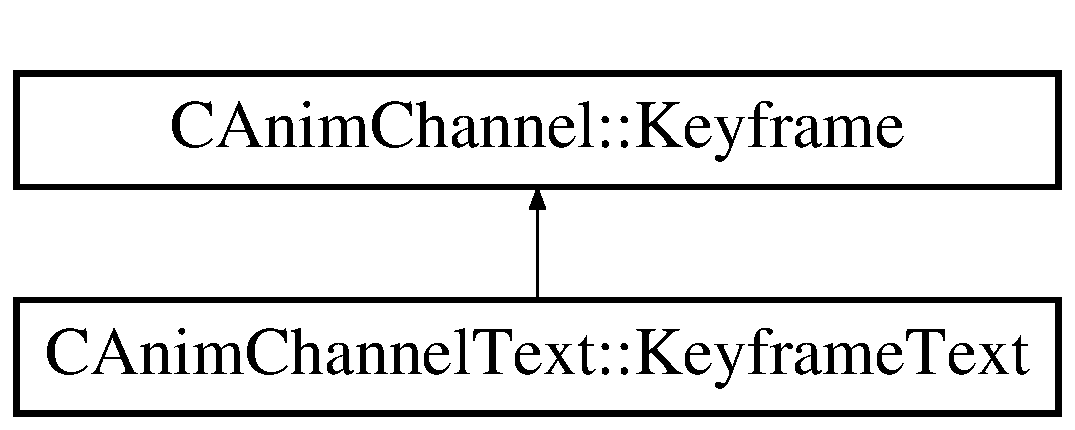
\includegraphics[height=2.000000cm]{class_c_anim_channel_text_1_1_keyframe_text}
\end{center}
\end{figure}
\subsection*{Public Member Functions}
\begin{DoxyCompactItemize}
\item 
\hyperlink{class_c_anim_channel_text_1_1_keyframe_text_a08c2025f5f3e5b1658f5e644f9da90c7}{Keyframe\+Text} (\hyperlink{class_c_anim_channel_text}{C\+Anim\+Channel\+Text} $\ast$channel, std\+::wstring text, bool mirror)
\begin{DoxyCompactList}\small\item\em Constructor. \end{DoxyCompactList}\item 
\hypertarget{class_c_anim_channel_text_1_1_keyframe_text_a9b020a2026e28bed8b748d7cf10b5c4c}{\hyperlink{class_c_anim_channel_text_1_1_keyframe_text_a9b020a2026e28bed8b748d7cf10b5c4c}{Keyframe\+Text} ()=delete}\label{class_c_anim_channel_text_1_1_keyframe_text_a9b020a2026e28bed8b748d7cf10b5c4c}

\begin{DoxyCompactList}\small\item\em Default constructor disabled. \end{DoxyCompactList}\item 
\hypertarget{class_c_anim_channel_text_1_1_keyframe_text_a364ca7bcbd1c8ff04811653130962a00}{\hyperlink{class_c_anim_channel_text_1_1_keyframe_text_a364ca7bcbd1c8ff04811653130962a00}{Keyframe\+Text} (const \hyperlink{class_c_anim_channel_text_1_1_keyframe_text}{Keyframe\+Text} \&)=delete}\label{class_c_anim_channel_text_1_1_keyframe_text_a364ca7bcbd1c8ff04811653130962a00}

\begin{DoxyCompactList}\small\item\em Copy constructor disabled. \end{DoxyCompactList}\item 
\hypertarget{class_c_anim_channel_text_1_1_keyframe_text_a1acfd06ff4f697cabdb2eac2a5cc43f0}{void \hyperlink{class_c_anim_channel_text_1_1_keyframe_text_a1acfd06ff4f697cabdb2eac2a5cc43f0}{operator=} (const \hyperlink{class_c_anim_channel_text_1_1_keyframe_text}{Keyframe\+Text} \&)=delete}\label{class_c_anim_channel_text_1_1_keyframe_text_a1acfd06ff4f697cabdb2eac2a5cc43f0}

\begin{DoxyCompactList}\small\item\em Assignment operator disabled. \end{DoxyCompactList}\item 
std\+::wstring \hyperlink{class_c_anim_channel_text_1_1_keyframe_text_a37c016c705e54ec26408d4ac9e710610}{Get\+Text} ()
\begin{DoxyCompactList}\small\item\em Get the text at this keyframe. \end{DoxyCompactList}\item 
bool \hyperlink{class_c_anim_channel_text_1_1_keyframe_text_a22e197234db7f95ed36f3dcbd0c53fcd}{Get\+Mirror} ()
\begin{DoxyCompactList}\small\item\em Get if the text bubble is mirrored or not at this keyframe. \end{DoxyCompactList}\item 
\hypertarget{class_c_anim_channel_text_1_1_keyframe_text_aafb866f2e2de274f46199fe1be0ec485}{virtual void \hyperlink{class_c_anim_channel_text_1_1_keyframe_text_aafb866f2e2de274f46199fe1be0ec485}{Use\+As1} () override}\label{class_c_anim_channel_text_1_1_keyframe_text_aafb866f2e2de274f46199fe1be0ec485}

\begin{DoxyCompactList}\small\item\em Use this keyframe as keyframe 1. \end{DoxyCompactList}\item 
\hypertarget{class_c_anim_channel_text_1_1_keyframe_text_a26c8a71bab1e9b11e6d80bc25cda7242}{virtual void \hyperlink{class_c_anim_channel_text_1_1_keyframe_text_a26c8a71bab1e9b11e6d80bc25cda7242}{Use\+As2} () override}\label{class_c_anim_channel_text_1_1_keyframe_text_a26c8a71bab1e9b11e6d80bc25cda7242}

\begin{DoxyCompactList}\small\item\em Use this keyframe as keyfraem 2. \end{DoxyCompactList}\item 
\hypertarget{class_c_anim_channel_text_1_1_keyframe_text_a5dd278fa5bc6a275a8efc48ad13405b1}{virtual void \hyperlink{class_c_anim_channel_text_1_1_keyframe_text_a5dd278fa5bc6a275a8efc48ad13405b1}{Use\+Only} () override}\label{class_c_anim_channel_text_1_1_keyframe_text_a5dd278fa5bc6a275a8efc48ad13405b1}

\begin{DoxyCompactList}\small\item\em Use this keyframe as the angle. \end{DoxyCompactList}\item 
virtual std\+::shared\+\_\+ptr\\*
$<$ \hyperlink{classxmlnode_1_1_c_xml_node}{xmlnode\+::\+C\+Xml\+Node} $>$ \hyperlink{class_c_anim_channel_text_1_1_keyframe_text_a502cf5d31023f7d1272c4e1a85f94e31}{Xml\+Save} (const std\+::shared\+\_\+ptr$<$ \hyperlink{classxmlnode_1_1_c_xml_node}{xmlnode\+::\+C\+Xml\+Node} $>$ \&node)
\begin{DoxyCompactList}\small\item\em Function to save the text in this keyfram. \end{DoxyCompactList}\end{DoxyCompactItemize}
\subsection*{Additional Inherited Members}


\subsection{Detailed Description}
A ket frame for the text channel. 

\subsection{Constructor \& Destructor Documentation}
\hypertarget{class_c_anim_channel_text_1_1_keyframe_text_a08c2025f5f3e5b1658f5e644f9da90c7}{\index{C\+Anim\+Channel\+Text\+::\+Keyframe\+Text@{C\+Anim\+Channel\+Text\+::\+Keyframe\+Text}!Keyframe\+Text@{Keyframe\+Text}}
\index{Keyframe\+Text@{Keyframe\+Text}!C\+Anim\+Channel\+Text\+::\+Keyframe\+Text@{C\+Anim\+Channel\+Text\+::\+Keyframe\+Text}}
\subsubsection[{Keyframe\+Text}]{\setlength{\rightskip}{0pt plus 5cm}C\+Anim\+Channel\+Text\+::\+Keyframe\+Text\+::\+Keyframe\+Text (
\begin{DoxyParamCaption}
\item[{{\bf C\+Anim\+Channel\+Text} $\ast$}]{channel, }
\item[{std\+::wstring}]{text, }
\item[{bool}]{mirror}
\end{DoxyParamCaption}
)\hspace{0.3cm}{\ttfamily [inline]}}}\label{class_c_anim_channel_text_1_1_keyframe_text_a08c2025f5f3e5b1658f5e644f9da90c7}


Constructor. 


\begin{DoxyParams}{Parameters}
{\em channel} & The channel we are for \\
\hline
{\em text} & The text for the keyframe \\
\hline
{\em mirror} & is mirror or not for the keyframe \\
\hline
\end{DoxyParams}


\subsection{Member Function Documentation}
\hypertarget{class_c_anim_channel_text_1_1_keyframe_text_a22e197234db7f95ed36f3dcbd0c53fcd}{\index{C\+Anim\+Channel\+Text\+::\+Keyframe\+Text@{C\+Anim\+Channel\+Text\+::\+Keyframe\+Text}!Get\+Mirror@{Get\+Mirror}}
\index{Get\+Mirror@{Get\+Mirror}!C\+Anim\+Channel\+Text\+::\+Keyframe\+Text@{C\+Anim\+Channel\+Text\+::\+Keyframe\+Text}}
\subsubsection[{Get\+Mirror}]{\setlength{\rightskip}{0pt plus 5cm}bool C\+Anim\+Channel\+Text\+::\+Keyframe\+Text\+::\+Get\+Mirror (
\begin{DoxyParamCaption}
{}
\end{DoxyParamCaption}
)\hspace{0.3cm}{\ttfamily [inline]}}}\label{class_c_anim_channel_text_1_1_keyframe_text_a22e197234db7f95ed36f3dcbd0c53fcd}


Get if the text bubble is mirrored or not at this keyframe. 

\begin{DoxyReturn}{Returns}
true or not 
\end{DoxyReturn}
\hypertarget{class_c_anim_channel_text_1_1_keyframe_text_a37c016c705e54ec26408d4ac9e710610}{\index{C\+Anim\+Channel\+Text\+::\+Keyframe\+Text@{C\+Anim\+Channel\+Text\+::\+Keyframe\+Text}!Get\+Text@{Get\+Text}}
\index{Get\+Text@{Get\+Text}!C\+Anim\+Channel\+Text\+::\+Keyframe\+Text@{C\+Anim\+Channel\+Text\+::\+Keyframe\+Text}}
\subsubsection[{Get\+Text}]{\setlength{\rightskip}{0pt plus 5cm}std\+::wstring C\+Anim\+Channel\+Text\+::\+Keyframe\+Text\+::\+Get\+Text (
\begin{DoxyParamCaption}
{}
\end{DoxyParamCaption}
)\hspace{0.3cm}{\ttfamily [inline]}}}\label{class_c_anim_channel_text_1_1_keyframe_text_a37c016c705e54ec26408d4ac9e710610}


Get the text at this keyframe. 

\begin{DoxyReturn}{Returns}
text in string 
\end{DoxyReturn}
\hypertarget{class_c_anim_channel_text_1_1_keyframe_text_a502cf5d31023f7d1272c4e1a85f94e31}{\index{C\+Anim\+Channel\+Text\+::\+Keyframe\+Text@{C\+Anim\+Channel\+Text\+::\+Keyframe\+Text}!Xml\+Save@{Xml\+Save}}
\index{Xml\+Save@{Xml\+Save}!C\+Anim\+Channel\+Text\+::\+Keyframe\+Text@{C\+Anim\+Channel\+Text\+::\+Keyframe\+Text}}
\subsubsection[{Xml\+Save}]{\setlength{\rightskip}{0pt plus 5cm}std\+::shared\+\_\+ptr$<$ {\bf xmlnode\+::\+C\+Xml\+Node} $>$ C\+Anim\+Channel\+Text\+::\+Keyframe\+Text\+::\+Xml\+Save (
\begin{DoxyParamCaption}
\item[{const std\+::shared\+\_\+ptr$<$ {\bf xmlnode\+::\+C\+Xml\+Node} $>$ \&}]{node}
\end{DoxyParamCaption}
)\hspace{0.3cm}{\ttfamily [virtual]}}}\label{class_c_anim_channel_text_1_1_keyframe_text_a502cf5d31023f7d1272c4e1a85f94e31}


Function to save the text in this keyfram. 

Save this keyframe to an X\+M\+L node.


\begin{DoxyParams}{Parameters}
{\em node} & The node we are going to be a child of \\
\hline
\end{DoxyParams}
\begin{DoxyReturn}{Returns}
Allocated X\+M\+L node. 
\end{DoxyReturn}


Reimplemented from \hyperlink{class_c_anim_channel_1_1_keyframe_a2dbc0b264510a45b9a429f64aa2d8448}{C\+Anim\+Channel\+::\+Keyframe}.



The documentation for this class was generated from the following files\+:\begin{DoxyCompactItemize}
\item 
\hyperlink{_anim_channel_text_8h}{Anim\+Channel\+Text.\+h}\item 
\hyperlink{_anim_channel_text_8cpp}{Anim\+Channel\+Text.\+cpp}\end{DoxyCompactItemize}

\chapter{File Documentation}
\hypertarget{_actor_8cpp}{\section{Actor.\+cpp File Reference}
\label{_actor_8cpp}\index{Actor.\+cpp@{Actor.\+cpp}}
}
{\ttfamily \#include \char`\"{}stdafx.\+h\char`\"{}}\\*
{\ttfamily \#include \char`\"{}Actor.\+h\char`\"{}}\\*
{\ttfamily \#include \char`\"{}Picture.\+h\char`\"{}}\\*
{\ttfamily \#include $<$sstream$>$}\\*


\subsection{Detailed Description}
\begin{DoxyAuthor}{Author}
Charles B. Owen 
\end{DoxyAuthor}

\hypertarget{_actor_8h}{\section{Actor.\+h File Reference}
\label{_actor_8h}\index{Actor.\+h@{Actor.\+h}}
}


Class for actors in our drawings.  


{\ttfamily \#include \char`\"{}Drawable.\+h\char`\"{}}\\*
{\ttfamily \#include \char`\"{}Anim\+Channel\+Point.\+h\char`\"{}}\\*
{\ttfamily \#include $<$string$>$}\\*
{\ttfamily \#include $<$memory$>$}\\*
{\ttfamily \#include $<$vector$>$}\\*
\subsection*{Classes}
\begin{DoxyCompactItemize}
\item 
class \hyperlink{class_c_actor}{C\+Actor}
\begin{DoxyCompactList}\small\item\em Class for actors in our drawings. \end{DoxyCompactList}\end{DoxyCompactItemize}


\subsection{Detailed Description}
Class for actors in our drawings. 

\begin{DoxyAuthor}{Author}
Charles B. Owen 
\end{DoxyAuthor}

\hypertarget{_actor_factory_8cpp}{\section{Actor\+Factory.\+cpp File Reference}
\label{_actor_factory_8cpp}\index{Actor\+Factory.\+cpp@{Actor\+Factory.\+cpp}}
}
{\ttfamily \#include \char`\"{}stdafx.\+h\char`\"{}}\\*
{\ttfamily \#include \char`\"{}Actor\+Factory.\+h\char`\"{}}\\*


\subsection{Detailed Description}
\begin{DoxyAuthor}{Author}
Charles B. Owen 
\end{DoxyAuthor}

\hypertarget{_actor_factory_8h}{\section{Actor\+Factory.\+h File Reference}
\label{_actor_factory_8h}\index{Actor\+Factory.\+h@{Actor\+Factory.\+h}}
}


Abstract base class for actor factories.  


{\ttfamily \#include $<$memory$>$}\\*
{\ttfamily \#include \char`\"{}Actor.\+h\char`\"{}}\\*
\subsection*{Classes}
\begin{DoxyCompactItemize}
\item 
class \hyperlink{class_c_actor_factory}{C\+Actor\+Factory}
\begin{DoxyCompactList}\small\item\em Abstract base class for actor factories. \end{DoxyCompactList}\end{DoxyCompactItemize}


\subsection{Detailed Description}
Abstract base class for actor factories. 

\begin{DoxyAuthor}{Author}
Charles B. Owen 
\end{DoxyAuthor}

\hypertarget{_anim_channel_8cpp}{\section{Anim\+Channel.\+cpp File Reference}
\label{_anim_channel_8cpp}\index{Anim\+Channel.\+cpp@{Anim\+Channel.\+cpp}}
}
{\ttfamily \#include \char`\"{}stdafx.\+h\char`\"{}}\\*
{\ttfamily \#include \char`\"{}Anim\+Channel.\+h\char`\"{}}\\*
{\ttfamily \#include \char`\"{}Timeline.\+h\char`\"{}}\\*


\subsection{Detailed Description}
\begin{DoxyAuthor}{Author}
Charles B. Owen 
\end{DoxyAuthor}

\hypertarget{_anim_channel_8h}{\section{Anim\+Channel.\+h File Reference}
\label{_anim_channel_8h}\index{Anim\+Channel.\+h@{Anim\+Channel.\+h}}
}


Base class for an animation channel.  


{\ttfamily \#include $<$string$>$}\\*
{\ttfamily \#include $<$vector$>$}\\*
{\ttfamily \#include $<$memory$>$}\\*
{\ttfamily \#include \char`\"{}Xml\+Node.\+h\char`\"{}}\\*
\subsection*{Classes}
\begin{DoxyCompactItemize}
\item 
class \hyperlink{class_c_anim_channel}{C\+Anim\+Channel}
\begin{DoxyCompactList}\small\item\em Base class for an animation channel. \end{DoxyCompactList}\item 
class \hyperlink{class_c_anim_channel_1_1_keyframe}{C\+Anim\+Channel\+::\+Keyframe}
\begin{DoxyCompactList}\small\item\em Class that represents a keyframe. \end{DoxyCompactList}\end{DoxyCompactItemize}


\subsection{Detailed Description}
Base class for an animation channel. 

\begin{DoxyAuthor}{Author}
Charles B. Owen 
\end{DoxyAuthor}

\hypertarget{_anim_channel_angle_8cpp}{\section{Anim\+Channel\+Angle.\+cpp File Reference}
\label{_anim_channel_angle_8cpp}\index{Anim\+Channel\+Angle.\+cpp@{Anim\+Channel\+Angle.\+cpp}}
}
{\ttfamily \#include \char`\"{}stdafx.\+h\char`\"{}}\\*
{\ttfamily \#include \char`\"{}Anim\+Channel\+Angle.\+h\char`\"{}}\\*
{\ttfamily \#include \char`\"{}Timeline.\+h\char`\"{}}\\*


\subsection{Detailed Description}
\begin{DoxyAuthor}{Author}
Charles B. Owen 
\end{DoxyAuthor}

\hypertarget{_anim_channel_angle_8h}{\section{Anim\+Channel\+Angle.\+h File Reference}
\label{_anim_channel_angle_8h}\index{Anim\+Channel\+Angle.\+h@{Anim\+Channel\+Angle.\+h}}
}


Animation channel for angles.  


{\ttfamily \#include \char`\"{}Anim\+Channel.\+h\char`\"{}}\\*
\subsection*{Classes}
\begin{DoxyCompactItemize}
\item 
class \hyperlink{class_c_anim_channel_angle}{C\+Anim\+Channel\+Angle}
\begin{DoxyCompactList}\small\item\em Animation channel for angles. \end{DoxyCompactList}\item 
class \hyperlink{class_c_anim_channel_angle_1_1_keyframe_angle}{C\+Anim\+Channel\+Angle\+::\+Keyframe\+Angle}
\begin{DoxyCompactList}\small\item\em A keyframe for an angle channel. \end{DoxyCompactList}\end{DoxyCompactItemize}


\subsection{Detailed Description}
Animation channel for angles. 

\begin{DoxyAuthor}{Author}
Charles B. Owen 
\end{DoxyAuthor}

\hypertarget{_anim_channel_point_8cpp}{\section{Anim\+Channel\+Point.\+cpp File Reference}
\label{_anim_channel_point_8cpp}\index{Anim\+Channel\+Point.\+cpp@{Anim\+Channel\+Point.\+cpp}}
}
{\ttfamily \#include \char`\"{}stdafx.\+h\char`\"{}}\\*
{\ttfamily \#include \char`\"{}Anim\+Channel\+Point.\+h\char`\"{}}\\*
{\ttfamily \#include \char`\"{}Timeline.\+h\char`\"{}}\\*


\subsection{Detailed Description}
\begin{DoxyAuthor}{Author}
Charles B. Owen 
\end{DoxyAuthor}

\hypertarget{_anim_channel_point_8h}{\section{Anim\+Channel\+Point.\+h File Reference}
\label{_anim_channel_point_8h}\index{Anim\+Channel\+Point.\+h@{Anim\+Channel\+Point.\+h}}
}


An animation channel specific to points (movement)  


{\ttfamily \#include \char`\"{}Anim\+Channel.\+h\char`\"{}}\\*
\subsection*{Classes}
\begin{DoxyCompactItemize}
\item 
class \hyperlink{class_c_anim_channel_point}{C\+Anim\+Channel\+Point}
\begin{DoxyCompactList}\small\item\em An animation channel specific to points (movement) \end{DoxyCompactList}\item 
class \hyperlink{class_c_anim_channel_point_1_1_keyframe_point}{C\+Anim\+Channel\+Point\+::\+Keyframe\+Point}
\begin{DoxyCompactList}\small\item\em A keyframe for a point channel. \end{DoxyCompactList}\end{DoxyCompactItemize}


\subsection{Detailed Description}
An animation channel specific to points (movement) 

\begin{DoxyAuthor}{Author}
Charles B. Owen 
\end{DoxyAuthor}

\hypertarget{_anim_channel_text_8cpp}{\section{Anim\+Channel\+Text.\+cpp File Reference}
\label{_anim_channel_text_8cpp}\index{Anim\+Channel\+Text.\+cpp@{Anim\+Channel\+Text.\+cpp}}
}
{\ttfamily \#include \char`\"{}stdafx.\+h\char`\"{}}\\*
{\ttfamily \#include \char`\"{}Anim\+Channel\+Text.\+h\char`\"{}}\\*
{\ttfamily \#include \char`\"{}Timeline.\+h\char`\"{}}\\*


\subsection{Detailed Description}
\begin{DoxyAuthor}{Author}
Yiming Li 
\end{DoxyAuthor}

\hypertarget{_anim_channel_text_8h}{\section{Anim\+Channel\+Text.\+h File Reference}
\label{_anim_channel_text_8h}\index{Anim\+Channel\+Text.\+h@{Anim\+Channel\+Text.\+h}}
}


The Anim\+Channel Class to edit the text in the text bubble during the animation.  


{\ttfamily \#include \char`\"{}Anim\+Channel.\+h\char`\"{}}\\*
\subsection*{Classes}
\begin{DoxyCompactItemize}
\item 
class \hyperlink{class_c_anim_channel_text}{C\+Anim\+Channel\+Text}
\item 
class \hyperlink{class_c_anim_channel_text_1_1_keyframe_text}{C\+Anim\+Channel\+Text\+::\+Keyframe\+Text}
\begin{DoxyCompactList}\small\item\em A ket frame for the text channel. \end{DoxyCompactList}\end{DoxyCompactItemize}


\subsection{Detailed Description}
The Anim\+Channel Class to edit the text in the text bubble during the animation. 

\begin{DoxyAuthor}{Author}
Yiming Li 
\end{DoxyAuthor}

\hypertarget{_canadian_experience_8cpp}{\section{Canadian\+Experience.\+cpp File Reference}
\label{_canadian_experience_8cpp}\index{Canadian\+Experience.\+cpp@{Canadian\+Experience.\+cpp}}
}
{\ttfamily \#include \char`\"{}stdafx.\+h\char`\"{}}\\*
{\ttfamily \#include \char`\"{}afxwinappex.\+h\char`\"{}}\\*
{\ttfamily \#include \char`\"{}afxdialogex.\+h\char`\"{}}\\*
{\ttfamily \#include \char`\"{}Canadian\+Experience.\+h\char`\"{}}\\*
{\ttfamily \#include \char`\"{}Main\+Frm.\+h\char`\"{}}\\*
\subsection*{Classes}
\begin{DoxyCompactItemize}
\item 
class \hyperlink{class_c_about_dlg}{C\+About\+Dlg}
\begin{DoxyCompactList}\small\item\em The About dialog box. \end{DoxyCompactList}\end{DoxyCompactItemize}
\subsection*{Variables}
\begin{DoxyCompactItemize}
\item 
\hypertarget{_canadian_experience_8cpp_a67124bfb0809a8ff695444fd678f7a94}{\hyperlink{class_c_canadian_experience_app}{C\+Canadian\+Experience\+App} \hyperlink{_canadian_experience_8cpp_a67124bfb0809a8ff695444fd678f7a94}{the\+App}}\label{_canadian_experience_8cpp_a67124bfb0809a8ff695444fd678f7a94}

\begin{DoxyCompactList}\small\item\em The one and only \hyperlink{class_c_canadian_experience_app}{C\+Canadian\+Experience\+App} object. \end{DoxyCompactList}\end{DoxyCompactItemize}


\subsection{Detailed Description}
\begin{DoxyAuthor}{Author}

\end{DoxyAuthor}

\hypertarget{_canadian_experience_8h}{\section{Canadian\+Experience.\+h File Reference}
\label{_canadian_experience_8h}\index{Canadian\+Experience.\+h@{Canadian\+Experience.\+h}}
}


Program application class.  


{\ttfamily \#include \char`\"{}resource.\+h\char`\"{}}\\*
\subsection*{Classes}
\begin{DoxyCompactItemize}
\item 
class \hyperlink{class_c_canadian_experience_app}{C\+Canadian\+Experience\+App}
\begin{DoxyCompactList}\small\item\em Program application class. \end{DoxyCompactList}\end{DoxyCompactItemize}
\subsection*{Variables}
\begin{DoxyCompactItemize}
\item 
\hypertarget{_canadian_experience_8h_a67124bfb0809a8ff695444fd678f7a94}{\hyperlink{class_c_canadian_experience_app}{C\+Canadian\+Experience\+App} \hyperlink{_canadian_experience_8h_a67124bfb0809a8ff695444fd678f7a94}{the\+App}}\label{_canadian_experience_8h_a67124bfb0809a8ff695444fd678f7a94}

\begin{DoxyCompactList}\small\item\em The one and only \hyperlink{class_c_canadian_experience_app}{C\+Canadian\+Experience\+App} object. \end{DoxyCompactList}\end{DoxyCompactItemize}


\subsection{Detailed Description}
Program application class. 

\begin{DoxyAuthor}{Author}

\end{DoxyAuthor}

\hypertarget{_double_buffer_d_c_8h}{\section{Double\+Buffer\+D\+C.\+h File Reference}
\label{_double_buffer_d_c_8h}\index{Double\+Buffer\+D\+C.\+h@{Double\+Buffer\+D\+C.\+h}}
}


Customer device context that supports double buffering.  




\subsection{Detailed Description}
Customer device context that supports double buffering. 


\hypertarget{_drawable_8cpp}{\section{Drawable.\+cpp File Reference}
\label{_drawable_8cpp}\index{Drawable.\+cpp@{Drawable.\+cpp}}
}
{\ttfamily \#include \char`\"{}stdafx.\+h\char`\"{}}\\*
{\ttfamily \#include \char`\"{}Drawable.\+h\char`\"{}}\\*
{\ttfamily \#include $<$cmath$>$}\\*
{\ttfamily \#include \char`\"{}Actor.\+h\char`\"{}}\\*
{\ttfamily \#include \char`\"{}Timeline.\+h\char`\"{}}\\*


\subsection{Detailed Description}
\begin{DoxyAuthor}{Author}
Charles B. Owen 
\end{DoxyAuthor}

\hypertarget{_drawable_8h}{\section{Drawable.\+h File Reference}
\label{_drawable_8h}\index{Drawable.\+h@{Drawable.\+h}}
}


Abstract base class for drawable elements of our picture.  


{\ttfamily \#include $<$memory$>$}\\*
{\ttfamily \#include $<$string$>$}\\*
{\ttfamily \#include $<$vector$>$}\\*
{\ttfamily \#include \char`\"{}Text\+Bubble.\+h\char`\"{}}\\*
{\ttfamily \#include \char`\"{}Anim\+Channel\+Angle.\+h\char`\"{}}\\*
\subsection*{Classes}
\begin{DoxyCompactItemize}
\item 
class \hyperlink{class_c_drawable}{C\+Drawable}
\begin{DoxyCompactList}\small\item\em Abstract base class for drawable elements of our picture. \end{DoxyCompactList}\item 
class \hyperlink{class_c_drawable_1_1_child_iter}{C\+Drawable\+::\+Child\+Iter}
\begin{DoxyCompactList}\small\item\em Iterator that iterates over the children of this drawable. \end{DoxyCompactList}\end{DoxyCompactItemize}


\subsection{Detailed Description}
Abstract base class for drawable elements of our picture. 

\begin{DoxyAuthor}{Author}
Charles B. Owen 
\end{DoxyAuthor}

\hypertarget{_harold_factory_8cpp}{\section{Harold\+Factory.\+cpp File Reference}
\label{_harold_factory_8cpp}\index{Harold\+Factory.\+cpp@{Harold\+Factory.\+cpp}}
}
{\ttfamily \#include \char`\"{}stdafx.\+h\char`\"{}}\\*
{\ttfamily \#include \char`\"{}Harold\+Factory.\+h\char`\"{}}\\*
{\ttfamily \#include \char`\"{}Poly\+Drawable.\+h\char`\"{}}\\*
{\ttfamily \#include \char`\"{}Image\+Drawable.\+h\char`\"{}}\\*
{\ttfamily \#include \char`\"{}Text\+Bubble\+Drawable.\+h\char`\"{}}\\*
{\ttfamily \#include \char`\"{}Head\+Top.\+h\char`\"{}}\\*


\subsection{Detailed Description}
\begin{DoxyAuthor}{Author}
Charles B. Owen 
\end{DoxyAuthor}

\hypertarget{_harold_factory_8h}{\section{Harold\+Factory.\+h File Reference}
\label{_harold_factory_8h}\index{Harold\+Factory.\+h@{Harold\+Factory.\+h}}
}


Factory class that builds the Harold character.  


{\ttfamily \#include \char`\"{}Actor\+Factory.\+h\char`\"{}}\\*
\subsection*{Classes}
\begin{DoxyCompactItemize}
\item 
class \hyperlink{class_c_harold_factory}{C\+Harold\+Factory}
\begin{DoxyCompactList}\small\item\em Factory class that builds the Harold character. \end{DoxyCompactList}\end{DoxyCompactItemize}


\subsection{Detailed Description}
Factory class that builds the Harold character. 

\begin{DoxyAuthor}{Author}
Charles B. Owen 
\end{DoxyAuthor}

\hypertarget{_head_top_8h}{\section{Head\+Top.\+h File Reference}
\label{_head_top_8h}\index{Head\+Top.\+h@{Head\+Top.\+h}}
}


Implements the top of a characters head, which has special functionality.  


{\ttfamily \#include \char`\"{}Image\+Drawable.\+h\char`\"{}}\\*
{\ttfamily \#include \char`\"{}Anim\+Channel\+Point.\+h\char`\"{}}\\*
\subsection*{Classes}
\begin{DoxyCompactItemize}
\item 
class \hyperlink{class_c_head_top}{C\+Head\+Top}
\begin{DoxyCompactList}\small\item\em Implements the top of a characters head, which has special functionality. \end{DoxyCompactList}\end{DoxyCompactItemize}


\subsection{Detailed Description}
Implements the top of a characters head, which has special functionality. 

\begin{DoxyAuthor}{Author}
Charles B. Owen 
\end{DoxyAuthor}

\hypertarget{_image_drawable_8cpp}{\section{Image\+Drawable.\+cpp File Reference}
\label{_image_drawable_8cpp}\index{Image\+Drawable.\+cpp@{Image\+Drawable.\+cpp}}
}
{\ttfamily \#include \char`\"{}stdafx.\+h\char`\"{}}\\*
{\ttfamily \#include \char`\"{}Image\+Drawable.\+h\char`\"{}}\\*
\subsection*{Variables}
\begin{DoxyCompactItemize}
\item 
\hypertarget{_image_drawable_8cpp_ade10fdf328965f595a01ff78f9f8dcc0}{const double \hyperlink{_image_drawable_8cpp_ade10fdf328965f595a01ff78f9f8dcc0}{Rto\+D} = 57.\+295779513}\label{_image_drawable_8cpp_ade10fdf328965f595a01ff78f9f8dcc0}

\begin{DoxyCompactList}\small\item\em Constant ratio to convert radians to degrees. \end{DoxyCompactList}\end{DoxyCompactItemize}


\subsection{Detailed Description}
\begin{DoxyAuthor}{Author}
Charles B. Owen 
\end{DoxyAuthor}

\hypertarget{_image_drawable_8h}{\section{Image\+Drawable.\+h File Reference}
\label{_image_drawable_8h}\index{Image\+Drawable.\+h@{Image\+Drawable.\+h}}
}


A drawable based on drawing a bitmap image.  


{\ttfamily \#include \char`\"{}Drawable.\+h\char`\"{}}\\*
{\ttfamily \#include \char`\"{}Rotated\+Bitmap.\+h\char`\"{}}\\*
\subsection*{Classes}
\begin{DoxyCompactItemize}
\item 
class \hyperlink{class_c_image_drawable}{C\+Image\+Drawable}
\begin{DoxyCompactList}\small\item\em A drawable based on drawing a bitmap image. \end{DoxyCompactList}\end{DoxyCompactItemize}


\subsection{Detailed Description}
A drawable based on drawing a bitmap image. 

\begin{DoxyAuthor}{Author}
Charles B. Owen 
\end{DoxyAuthor}

\hypertarget{_knife_8cpp}{\section{Knife.\+cpp File Reference}
\label{_knife_8cpp}\index{Knife.\+cpp@{Knife.\+cpp}}
}
{\ttfamily \#include \char`\"{}stdafx.\+h\char`\"{}}\\*
{\ttfamily \#include \char`\"{}Knife.\+h\char`\"{}}\\*
{\ttfamily \#include \char`\"{}Actor.\+h\char`\"{}}\\*
{\ttfamily \#include \char`\"{}Timeline.\+h\char`\"{}}\\*
{\ttfamily \#include $<$sstream$>$}\\*
{\ttfamily \#include $<$iomanip$>$}\\*
\subsection*{Variables}
\begin{DoxyCompactItemize}
\item 
\hypertarget{_knife_8cpp_ade10fdf328965f595a01ff78f9f8dcc0}{const double \hyperlink{_knife_8cpp_ade10fdf328965f595a01ff78f9f8dcc0}{Rto\+D} = 57.\+295779513}\label{_knife_8cpp_ade10fdf328965f595a01ff78f9f8dcc0}

\begin{DoxyCompactList}\small\item\em Constant ratio to convert radians to degrees. \end{DoxyCompactList}\end{DoxyCompactItemize}


\subsection{Detailed Description}
\begin{DoxyAuthor}{Author}
Yiming Li 
\end{DoxyAuthor}

\hypertarget{_knife_8h}{\section{Knife.\+h File Reference}
\label{_knife_8h}\index{Knife.\+h@{Knife.\+h}}
}


Implement a knife for sparty.  


{\ttfamily \#include \char`\"{}Image\+Drawable.\+h\char`\"{}}\\*
{\ttfamily \#include \char`\"{}Anim\+Channel\+Point.\+h\char`\"{}}\\*
\subsection*{Classes}
\begin{DoxyCompactItemize}
\item 
class \hyperlink{class_c_knife}{C\+Knife}
\begin{DoxyCompactList}\small\item\em Implemnet the knife for sparty. \end{DoxyCompactList}\end{DoxyCompactItemize}


\subsection{Detailed Description}
Implement a knife for sparty. 

\begin{DoxyAuthor}{Author}
Yiming Li 
\end{DoxyAuthor}

\hypertarget{_linked_list_8cpp}{\section{Linked\+List.\+cpp File Reference}
\label{_linked_list_8cpp}\index{Linked\+List.\+cpp@{Linked\+List.\+cpp}}
}
{\ttfamily \#include \char`\"{}stdafx.\+h\char`\"{}}\\*
{\ttfamily \#include \char`\"{}Linked\+List.\+h\char`\"{}}\\*


\subsection{Detailed Description}
\begin{DoxyAuthor}{Author}
Yiming Li 
\end{DoxyAuthor}

\hypertarget{_linked_list_8h}{\section{Linked\+List.\+h File Reference}
\label{_linked_list_8h}\index{Linked\+List.\+h@{Linked\+List.\+h}}
}


The linked list to store the snowflake.  


{\ttfamily \#include \char`\"{}Snowflake.\+h\char`\"{}}\\*
{\ttfamily \#include $<$memory$>$}\\*
\subsection*{Classes}
\begin{DoxyCompactItemize}
\item 
class \hyperlink{class_c_linked_list}{C\+Linked\+List}
\begin{DoxyCompactList}\small\item\em The linked calss to store the snow flakes. \end{DoxyCompactList}\end{DoxyCompactItemize}


\subsection{Detailed Description}
The linked list to store the snowflake. 

\begin{DoxyAuthor}{Author}
Yiming Li 
\end{DoxyAuthor}

\hypertarget{_main_frm_8cpp}{\section{Main\+Frm.\+cpp File Reference}
\label{_main_frm_8cpp}\index{Main\+Frm.\+cpp@{Main\+Frm.\+cpp}}
}
{\ttfamily \#include \char`\"{}stdafx.\+h\char`\"{}}\\*
{\ttfamily \#include \char`\"{}Canadian\+Experience.\+h\char`\"{}}\\*
{\ttfamily \#include \char`\"{}Main\+Frm.\+h\char`\"{}}\\*
{\ttfamily \#include \char`\"{}View\+Top.\+h\char`\"{}}\\*
{\ttfamily \#include \char`\"{}Picture.\+h\char`\"{}}\\*
{\ttfamily \#include \char`\"{}Picture\+Factory.\+h\char`\"{}}\\*
{\ttfamily \#include \char`\"{}Timeline\+Dlg.\+h\char`\"{}}\\*
{\ttfamily \#include \char`\"{}Text\+Bubble\+Dlg.\+h\char`\"{}}\\*
{\ttfamily \#include \char`\"{}Actor.\+h\char`\"{}}\\*


\subsection{Detailed Description}
Implementation of the \hyperlink{class_c_main_frame}{C\+Main\+Frame} class \begin{DoxyAuthor}{Author}
Yiming Li 
\end{DoxyAuthor}

\hypertarget{_main_frm_8h}{\section{Main\+Frm.\+h File Reference}
\label{_main_frm_8h}\index{Main\+Frm.\+h@{Main\+Frm.\+h}}
}


The program main frame.  


{\ttfamily \#include \char`\"{}View\+Edit.\+h\char`\"{}}\\*
{\ttfamily \#include \char`\"{}View\+Timeline.\+h\char`\"{}}\\*
{\ttfamily \#include \char`\"{}View\+Actors.\+h\char`\"{}}\\*
{\ttfamily \#include \char`\"{}Particle\+System.\+h\char`\"{}}\\*
{\ttfamily \#include $<$memory$>$}\\*
\subsection*{Classes}
\begin{DoxyCompactItemize}
\item 
class \hyperlink{class_c_main_frame}{C\+Main\+Frame}
\begin{DoxyCompactList}\small\item\em Program main frame. \end{DoxyCompactList}\end{DoxyCompactItemize}


\subsection{Detailed Description}
The program main frame. 

\begin{DoxyAuthor}{Author}

\end{DoxyAuthor}

\hypertarget{_particle_system_8cpp}{\section{Particle\+System.\+cpp File Reference}
\label{_particle_system_8cpp}\index{Particle\+System.\+cpp@{Particle\+System.\+cpp}}
}
{\ttfamily \#include \char`\"{}stdafx.\+h\char`\"{}}\\*
{\ttfamily \#include \char`\"{}Particle\+System.\+h\char`\"{}}\\*
{\ttfamily \#include \char`\"{}Picture.\+h\char`\"{}}\\*
{\ttfamily \#include $<$vector$>$}\\*


\subsection{Detailed Description}
\begin{DoxyAuthor}{Author}
Yiming Li 
\end{DoxyAuthor}

\hypertarget{_particle_system_8h}{\section{Particle\+System.\+h File Reference}
\label{_particle_system_8h}\index{Particle\+System.\+h@{Particle\+System.\+h}}
}


Class for particle syystem of snow operation.  


{\ttfamily \#include \char`\"{}Linked\+List.\+h\char`\"{}}\\*
{\ttfamily \#include \char`\"{}Snowflake.\+h\char`\"{}}\\*
\subsection*{Classes}
\begin{DoxyCompactItemize}
\item 
class \hyperlink{class_c_particle_system}{C\+Particle\+System}
\begin{DoxyCompactList}\small\item\em The Particle\+System to implement the snow draw and update. \end{DoxyCompactList}\end{DoxyCompactItemize}


\subsection{Detailed Description}
Class for particle syystem of snow operation. 

\begin{DoxyAuthor}{Author}
Yiming Li 
\end{DoxyAuthor}

\hypertarget{_picture_8cpp}{\section{Picture.\+cpp File Reference}
\label{_picture_8cpp}\index{Picture.\+cpp@{Picture.\+cpp}}
}
{\ttfamily \#include \char`\"{}stdafx.\+h\char`\"{}}\\*
{\ttfamily \#include \char`\"{}Picture.\+h\char`\"{}}\\*
{\ttfamily \#include \char`\"{}Actor.\+h\char`\"{}}\\*


\subsection{Detailed Description}
\begin{DoxyAuthor}{Author}
Charles B. Owen 
\end{DoxyAuthor}

\hypertarget{_picture_8h}{\section{Picture.\+h File Reference}
\label{_picture_8h}\index{Picture.\+h@{Picture.\+h}}
}


The picture we are drawing.  


{\ttfamily \#include $<$vector$>$}\\*
{\ttfamily \#include \char`\"{}Picture\+Observer.\+h\char`\"{}}\\*
{\ttfamily \#include \char`\"{}Timeline.\+h\char`\"{}}\\*
{\ttfamily \#include \char`\"{}Particle\+System.\+h\char`\"{}}\\*
{\ttfamily \#include \char`\"{}Main\+Frm.\+h\char`\"{}}\\*
\subsection*{Classes}
\begin{DoxyCompactItemize}
\item 
class \hyperlink{class_c_picture}{C\+Picture}
\begin{DoxyCompactList}\small\item\em The picture we are drawing. \end{DoxyCompactList}\item 
class \hyperlink{class_c_picture_1_1_actor_iter}{C\+Picture\+::\+Actor\+Iter}
\begin{DoxyCompactList}\small\item\em Iterator that iterates over the actors in a picture. \end{DoxyCompactList}\end{DoxyCompactItemize}


\subsection{Detailed Description}
The picture we are drawing. 

\begin{DoxyAuthor}{Author}
Charles B. Owen 
\end{DoxyAuthor}

\hypertarget{_picture_factory_8cpp}{\section{Picture\+Factory.\+cpp File Reference}
\label{_picture_factory_8cpp}\index{Picture\+Factory.\+cpp@{Picture\+Factory.\+cpp}}
}
{\ttfamily \#include \char`\"{}stdafx.\+h\char`\"{}}\\*
{\ttfamily \#include \char`\"{}Picture\+Factory.\+h\char`\"{}}\\*
{\ttfamily \#include \char`\"{}Harold\+Factory.\+h\char`\"{}}\\*
{\ttfamily \#include \char`\"{}Sparty\+Factory.\+h\char`\"{}}\\*
{\ttfamily \#include \char`\"{}Image\+Drawable.\+h\char`\"{}}\\*


\subsection{Detailed Description}
\begin{DoxyAuthor}{Author}
Charles B. Owen 
\end{DoxyAuthor}

\hypertarget{_picture_factory_8h}{\section{Picture\+Factory.\+h File Reference}
\label{_picture_factory_8h}\index{Picture\+Factory.\+h@{Picture\+Factory.\+h}}
}


A factory class that builds our picture.  


{\ttfamily \#include $<$memory$>$}\\*
{\ttfamily \#include \char`\"{}Picture.\+h\char`\"{}}\\*
\subsection*{Classes}
\begin{DoxyCompactItemize}
\item 
class \hyperlink{class_c_picture_factory}{C\+Picture\+Factory}
\begin{DoxyCompactList}\small\item\em A factory class that builds our picture. \end{DoxyCompactList}\end{DoxyCompactItemize}


\subsection{Detailed Description}
A factory class that builds our picture. 

\begin{DoxyAuthor}{Author}
Charles B. Owen 
\end{DoxyAuthor}

\hypertarget{_picture_observer_8cpp}{\section{Picture\+Observer.\+cpp File Reference}
\label{_picture_observer_8cpp}\index{Picture\+Observer.\+cpp@{Picture\+Observer.\+cpp}}
}
{\ttfamily \#include \char`\"{}stdafx.\+h\char`\"{}}\\*
{\ttfamily \#include \char`\"{}Picture\+Observer.\+h\char`\"{}}\\*
{\ttfamily \#include \char`\"{}Picture.\+h\char`\"{}}\\*


\subsection{Detailed Description}
\begin{DoxyAuthor}{Author}
Charles B. Owen 
\end{DoxyAuthor}

\hypertarget{_picture_observer_8h}{\section{Picture\+Observer.\+h File Reference}
\label{_picture_observer_8h}\index{Picture\+Observer.\+h@{Picture\+Observer.\+h}}
}


Observer base class for a picture.  


{\ttfamily \#include $<$memory$>$}\\*
\subsection*{Classes}
\begin{DoxyCompactItemize}
\item 
class \hyperlink{class_c_picture_observer}{C\+Picture\+Observer}
\begin{DoxyCompactList}\small\item\em Observer base class for a picture. \end{DoxyCompactList}\end{DoxyCompactItemize}


\subsection{Detailed Description}
Observer base class for a picture. 

\begin{DoxyAuthor}{Author}
Charles B. Owen 
\end{DoxyAuthor}

\hypertarget{_poly_drawable_8cpp}{\section{Poly\+Drawable.\+cpp File Reference}
\label{_poly_drawable_8cpp}\index{Poly\+Drawable.\+cpp@{Poly\+Drawable.\+cpp}}
}
{\ttfamily \#include \char`\"{}stdafx.\+h\char`\"{}}\\*
{\ttfamily \#include \char`\"{}Poly\+Drawable.\+h\char`\"{}}\\*


\subsection{Detailed Description}
\begin{DoxyAuthor}{Author}
Charles B. Owen 
\end{DoxyAuthor}

\hypertarget{_poly_drawable_8h}{\section{Poly\+Drawable.\+h File Reference}
\label{_poly_drawable_8h}\index{Poly\+Drawable.\+h@{Poly\+Drawable.\+h}}
}


A drawable based on polygon images.  


{\ttfamily \#include \char`\"{}Drawable.\+h\char`\"{}}\\*
{\ttfamily \#include $<$vector$>$}\\*
\subsection*{Classes}
\begin{DoxyCompactItemize}
\item 
class \hyperlink{class_c_poly_drawable}{C\+Poly\+Drawable}
\begin{DoxyCompactList}\small\item\em A drawable based on polygon images. \end{DoxyCompactList}\end{DoxyCompactItemize}


\subsection{Detailed Description}
A drawable based on polygon images. 

\begin{DoxyAuthor}{Author}
Charles B. Owen 
\end{DoxyAuthor}

\hypertarget{_rotated_bitmap_8cpp}{\section{Rotated\+Bitmap.\+cpp File Reference}
\label{_rotated_bitmap_8cpp}\index{Rotated\+Bitmap.\+cpp@{Rotated\+Bitmap.\+cpp}}
}
{\ttfamily \#include \char`\"{}stdafx.\+h\char`\"{}}\\*
{\ttfamily \#include \char`\"{}Rotated\+Bitmap.\+h\char`\"{}}\\*
\subsection*{Variables}
\begin{DoxyCompactItemize}
\item 
\hypertarget{_rotated_bitmap_8cpp_ade10fdf328965f595a01ff78f9f8dcc0}{const double \hyperlink{_rotated_bitmap_8cpp_ade10fdf328965f595a01ff78f9f8dcc0}{Rto\+D} = 57.\+295779513}\label{_rotated_bitmap_8cpp_ade10fdf328965f595a01ff78f9f8dcc0}

\begin{DoxyCompactList}\small\item\em Constant ratio to convert radians to degrees. \end{DoxyCompactList}\end{DoxyCompactItemize}


\subsection{Detailed Description}
\begin{DoxyAuthor}{Author}
Charles B. Owen 
\end{DoxyAuthor}

\hypertarget{_rotated_bitmap_8h}{\section{Rotated\+Bitmap.\+h File Reference}
\label{_rotated_bitmap_8h}\index{Rotated\+Bitmap.\+h@{Rotated\+Bitmap.\+h}}
}


Base class for a rotated bitmap.  


{\ttfamily \#include $<$memory$>$}\\*
{\ttfamily \#include $<$string$>$}\\*
\subsection*{Classes}
\begin{DoxyCompactItemize}
\item 
class \hyperlink{class_c_rotated_bitmap}{C\+Rotated\+Bitmap}
\begin{DoxyCompactList}\small\item\em Base class for a rotated bitmap. \end{DoxyCompactList}\end{DoxyCompactItemize}


\subsection{Detailed Description}
Base class for a rotated bitmap. 

\begin{DoxyAuthor}{Author}
Charles B. Owen 
\end{DoxyAuthor}

\hypertarget{_snowflake_8cpp}{\section{Snowflake.\+cpp File Reference}
\label{_snowflake_8cpp}\index{Snowflake.\+cpp@{Snowflake.\+cpp}}
}
{\ttfamily \#include \char`\"{}stdafx.\+h\char`\"{}}\\*
{\ttfamily \#include \char`\"{}Snowflake.\+h\char`\"{}}\\*


\subsection{Detailed Description}
\begin{DoxyAuthor}{Author}
Yiming Li 
\end{DoxyAuthor}

\hypertarget{_snowflake_8h}{\section{Snowflake.\+h File Reference}
\label{_snowflake_8h}\index{Snowflake.\+h@{Snowflake.\+h}}
}


The snowfalke class to inplement the snow.  


{\ttfamily \#include $<$memory$>$}\\*
\subsection*{Classes}
\begin{DoxyCompactItemize}
\item 
class \hyperlink{class_c_snowflake}{C\+Snowflake}
\begin{DoxyCompactList}\small\item\em The snow flake class to implement snow. \end{DoxyCompactList}\end{DoxyCompactItemize}


\subsection{Detailed Description}
The snowfalke class to inplement the snow. 

\begin{DoxyAuthor}{Author}
Yiming Li 
\end{DoxyAuthor}

\hypertarget{_sparty_factory_8cpp}{\section{Sparty\+Factory.\+cpp File Reference}
\label{_sparty_factory_8cpp}\index{Sparty\+Factory.\+cpp@{Sparty\+Factory.\+cpp}}
}
{\ttfamily \#include \char`\"{}stdafx.\+h\char`\"{}}\\*
{\ttfamily \#include \char`\"{}Sparty\+Factory.\+h\char`\"{}}\\*
{\ttfamily \#include \char`\"{}Poly\+Drawable.\+h\char`\"{}}\\*
{\ttfamily \#include \char`\"{}Image\+Drawable.\+h\char`\"{}}\\*
{\ttfamily \#include \char`\"{}Head\+Top.\+h\char`\"{}}\\*
{\ttfamily \#include \char`\"{}Text\+Bubble\+Drawable.\+h\char`\"{}}\\*
{\ttfamily \#include \char`\"{}Knife.\+h\char`\"{}}\\*


\subsection{Detailed Description}
\begin{DoxyAuthor}{Author}
Charles B. Owen 
\end{DoxyAuthor}

\hypertarget{_sparty_factory_8h}{\section{Sparty\+Factory.\+h File Reference}
\label{_sparty_factory_8h}\index{Sparty\+Factory.\+h@{Sparty\+Factory.\+h}}
}


Factory that builds the Sparty actor.  


{\ttfamily \#include \char`\"{}Actor\+Factory.\+h\char`\"{}}\\*
{\ttfamily \#include \char`\"{}Text\+Bubble\+Drawable.\+h\char`\"{}}\\*
\subsection*{Classes}
\begin{DoxyCompactItemize}
\item 
class \hyperlink{class_c_sparty_factory}{C\+Sparty\+Factory}
\begin{DoxyCompactList}\small\item\em Factory that builds the Sparty actor. \end{DoxyCompactList}\end{DoxyCompactItemize}


\subsection{Detailed Description}
Factory that builds the Sparty actor. 

\begin{DoxyAuthor}{Author}
Charles B. Owen 
\end{DoxyAuthor}

\hypertarget{_text_bubble_drawable_8cpp}{\section{Text\+Bubble\+Drawable.\+cpp File Reference}
\label{_text_bubble_drawable_8cpp}\index{Text\+Bubble\+Drawable.\+cpp@{Text\+Bubble\+Drawable.\+cpp}}
}
{\ttfamily \#include \char`\"{}stdafx.\+h\char`\"{}}\\*
{\ttfamily \#include \char`\"{}Text\+Bubble\+Drawable.\+h\char`\"{}}\\*
{\ttfamily \#include \char`\"{}Timeline.\+h\char`\"{}}\\*
{\ttfamily \#include \char`\"{}Actor.\+h\char`\"{}}\\*


\subsection{Detailed Description}
\begin{DoxyAuthor}{Author}
Yiming Li 
\end{DoxyAuthor}

\hypertarget{_text_bubble_drawable_8h}{\section{Text\+Bubble\+Drawable.\+h File Reference}
\label{_text_bubble_drawable_8h}\index{Text\+Bubble\+Drawable.\+h@{Text\+Bubble\+Drawable.\+h}}
}


The Text Bubble adapater class derived from the Drawable class.  


{\ttfamily \#include \char`\"{}Drawable.\+h\char`\"{}}\\*
{\ttfamily \#include \char`\"{}Text\+Bubble.\+h\char`\"{}}\\*
{\ttfamily \#include \char`\"{}Anim\+Channel\+Point.\+h\char`\"{}}\\*
{\ttfamily \#include \char`\"{}Anim\+Channel\+Text.\+h\char`\"{}}\\*
\subsection*{Classes}
\begin{DoxyCompactItemize}
\item 
class \hyperlink{class_c_text_bubble_drawable}{C\+Text\+Bubble\+Drawable}
\begin{DoxyCompactList}\small\item\em The text bubble class adpater. \end{DoxyCompactList}\end{DoxyCompactItemize}


\subsection{Detailed Description}
The Text Bubble adapater class derived from the Drawable class. 

\begin{DoxyAuthor}{Author}
Yiming Li 
\end{DoxyAuthor}

\hypertarget{_timeline_8cpp}{\section{Timeline.\+cpp File Reference}
\label{_timeline_8cpp}\index{Timeline.\+cpp@{Timeline.\+cpp}}
}
{\ttfamily \#include \char`\"{}stdafx.\+h\char`\"{}}\\*
{\ttfamily \#include \char`\"{}Timeline.\+h\char`\"{}}\\*
{\ttfamily \#include \char`\"{}Xml\+Node.\+h\char`\"{}}\\*


\subsection{Detailed Description}
\begin{DoxyAuthor}{Author}
Charles B. Owen 
\end{DoxyAuthor}

\hypertarget{_timeline_8h}{\section{Timeline.\+h File Reference}
\label{_timeline_8h}\index{Timeline.\+h@{Timeline.\+h}}
}


The animation timeline class.  


{\ttfamily \#include $<$vector$>$}\\*
{\ttfamily \#include \char`\"{}Anim\+Channel.\+h\char`\"{}}\\*
{\ttfamily \#include \char`\"{}Xml\+Node.\+h\char`\"{}}\\*
\subsection*{Classes}
\begin{DoxyCompactItemize}
\item 
class \hyperlink{class_c_timeline}{C\+Timeline}
\begin{DoxyCompactList}\small\item\em The animation timeline class. \end{DoxyCompactList}\end{DoxyCompactItemize}


\subsection{Detailed Description}
The animation timeline class. 

\begin{DoxyAuthor}{Author}
Charles B. Owen 
\end{DoxyAuthor}

\hypertarget{_timeline_dlg_8cpp}{\section{Timeline\+Dlg.\+cpp File Reference}
\label{_timeline_dlg_8cpp}\index{Timeline\+Dlg.\+cpp@{Timeline\+Dlg.\+cpp}}
}
{\ttfamily \#include \char`\"{}stdafx.\+h\char`\"{}}\\*
{\ttfamily \#include \char`\"{}Canadian\+Experience.\+h\char`\"{}}\\*
{\ttfamily \#include \char`\"{}Timeline\+Dlg.\+h\char`\"{}}\\*
{\ttfamily \#include \char`\"{}afxdialogex.\+h\char`\"{}}\\*


\subsection{Detailed Description}
\begin{DoxyAuthor}{Author}
Charles B. Owen 
\end{DoxyAuthor}

\hypertarget{_timeline_dlg_8h}{\section{Timeline\+Dlg.\+h File Reference}
\label{_timeline_dlg_8h}\index{Timeline\+Dlg.\+h@{Timeline\+Dlg.\+h}}
}


The timeline parameters dialog box.  


{\ttfamily \#include \char`\"{}Timeline.\+h\char`\"{}}\\*
\subsection*{Classes}
\begin{DoxyCompactItemize}
\item 
class \hyperlink{class_c_timeline_dlg}{C\+Timeline\+Dlg}
\begin{DoxyCompactList}\small\item\em The timeline parameters dialog box. \end{DoxyCompactList}\end{DoxyCompactItemize}


\subsection{Detailed Description}
The timeline parameters dialog box. 

\begin{DoxyAuthor}{Author}
Charles B. Owen 
\end{DoxyAuthor}

\hypertarget{_view_actors_8cpp}{\section{View\+Actors.\+cpp File Reference}
\label{_view_actors_8cpp}\index{View\+Actors.\+cpp@{View\+Actors.\+cpp}}
}
{\ttfamily \#include \char`\"{}stdafx.\+h\char`\"{}}\\*
{\ttfamily \#include \char`\"{}Canadian\+Experience.\+h\char`\"{}}\\*
{\ttfamily \#include \char`\"{}View\+Actors.\+h\char`\"{}}\\*
{\ttfamily \#include \char`\"{}Double\+Buffer\+D\+C.\+h\char`\"{}}\\*
\subsection*{Variables}
\begin{DoxyCompactItemize}
\item 
\hypertarget{_view_actors_8cpp_a46393c2446c3a9f140f2279eaa4717d1}{const int \hyperlink{_view_actors_8cpp_a46393c2446c3a9f140f2279eaa4717d1}{Indent} = 10}\label{_view_actors_8cpp_a46393c2446c3a9f140f2279eaa4717d1}

\begin{DoxyCompactList}\small\item\em Drawables indentation. \end{DoxyCompactList}\end{DoxyCompactItemize}


\subsection{Detailed Description}
\begin{DoxyAuthor}{Author}
Charles B. Owen 
\end{DoxyAuthor}

\hypertarget{_view_actors_8h}{\section{View\+Actors.\+h File Reference}
\label{_view_actors_8h}\index{View\+Actors.\+h@{View\+Actors.\+h}}
}


Class that provides a view windows for actors.  


{\ttfamily \#include \char`\"{}Picture\+Observer.\+h\char`\"{}}\\*
{\ttfamily \#include \char`\"{}Drawable.\+h\char`\"{}}\\*
\subsection*{Classes}
\begin{DoxyCompactItemize}
\item 
class \hyperlink{class_c_view_actors}{C\+View\+Actors}
\begin{DoxyCompactList}\small\item\em Class that provides a view windows for actors. \end{DoxyCompactList}\end{DoxyCompactItemize}


\subsection{Detailed Description}
Class that provides a view windows for actors. 

\begin{DoxyAuthor}{Author}
Charles B. Owen 
\end{DoxyAuthor}

\hypertarget{_view_edit_8cpp}{\section{View\+Edit.\+cpp File Reference}
\label{_view_edit_8cpp}\index{View\+Edit.\+cpp@{View\+Edit.\+cpp}}
}
{\ttfamily \#include \char`\"{}stdafx.\+h\char`\"{}}\\*
{\ttfamily \#include \char`\"{}Canadian\+Experience.\+h\char`\"{}}\\*
{\ttfamily \#include \char`\"{}View\+Edit.\+h\char`\"{}}\\*
{\ttfamily \#include \char`\"{}Double\+Buffer\+D\+C.\+h\char`\"{}}\\*
{\ttfamily \#include \char`\"{}Main\+Frm.\+h\char`\"{}}\\*
{\ttfamily \#include \char`\"{}Picture.\+h\char`\"{}}\\*
{\ttfamily \#include \char`\"{}Actor.\+h\char`\"{}}\\*
\subsection*{Variables}
\begin{DoxyCompactItemize}
\item 
\hypertarget{_view_edit_8cpp_a5aad50df163545659b29dc0f88c8a2d4}{const double \hyperlink{_view_edit_8cpp_a5aad50df163545659b29dc0f88c8a2d4}{Rotation\+Scaling} = 0.\+02}\label{_view_edit_8cpp_a5aad50df163545659b29dc0f88c8a2d4}

\begin{DoxyCompactList}\small\item\em A scaling factor, converts mouse motion to rotation in radians. \end{DoxyCompactList}\end{DoxyCompactItemize}


\subsection{Detailed Description}
\begin{DoxyAuthor}{Author}
Charles B. Owen 
\end{DoxyAuthor}

\hypertarget{_view_edit_8h}{\section{View\+Edit.\+h File Reference}
\label{_view_edit_8h}\index{View\+Edit.\+h@{View\+Edit.\+h}}
}


View class the provides a window for editing our pixture.  


{\ttfamily \#include \char`\"{}Picture\+Observer.\+h\char`\"{}}\\*
{\ttfamily \#include \char`\"{}Drawable.\+h\char`\"{}}\\*
{\ttfamily \#include \char`\"{}Text\+Bubble.\+h\char`\"{}}\\*
\subsection*{Classes}
\begin{DoxyCompactItemize}
\item 
class \hyperlink{class_c_view_edit}{C\+View\+Edit}
\begin{DoxyCompactList}\small\item\em View class the provides a window for editing our pixture. \end{DoxyCompactList}\end{DoxyCompactItemize}


\subsection{Detailed Description}
View class the provides a window for editing our pixture. 

\begin{DoxyAuthor}{Author}
Charles B. Owen 
\end{DoxyAuthor}

\hypertarget{_view_timeline_8cpp}{\section{View\+Timeline.\+cpp File Reference}
\label{_view_timeline_8cpp}\index{View\+Timeline.\+cpp@{View\+Timeline.\+cpp}}
}
{\ttfamily \#include \char`\"{}stdafx.\+h\char`\"{}}\\*
{\ttfamily \#include \char`\"{}Canadian\+Experience.\+h\char`\"{}}\\*
{\ttfamily \#include \char`\"{}View\+Timeline.\+h\char`\"{}}\\*
{\ttfamily \#include \char`\"{}Double\+Buffer\+D\+C.\+h\char`\"{}}\\*
{\ttfamily \#include \char`\"{}Main\+Frm.\+h\char`\"{}}\\*
{\ttfamily \#include \char`\"{}Timeline.\+h\char`\"{}}\\*
{\ttfamily \#include \char`\"{}Picture.\+h\char`\"{}}\\*
{\ttfamily \#include \char`\"{}Actor.\+h\char`\"{}}\\*
{\ttfamily \#include $<$sstream$>$}\\*
\subsection*{Variables}
\begin{DoxyCompactItemize}
\item 
\hypertarget{_view_timeline_8cpp_a00c2e195d5351bdc92a84a7fc4c5a7c7}{const int \hyperlink{_view_timeline_8cpp_a00c2e195d5351bdc92a84a7fc4c5a7c7}{Window\+Height} = 65}\label{_view_timeline_8cpp_a00c2e195d5351bdc92a84a7fc4c5a7c7}

\begin{DoxyCompactList}\small\item\em The window height. \end{DoxyCompactList}\item 
\hypertarget{_view_timeline_8cpp_a74f095c6b0b9640491938519705f01d3}{const int \hyperlink{_view_timeline_8cpp_a74f095c6b0b9640491938519705f01d3}{Tick\+Spacing} = 3}\label{_view_timeline_8cpp_a74f095c6b0b9640491938519705f01d3}

\begin{DoxyCompactList}\small\item\em The spacing between ticks in the timeline. \end{DoxyCompactList}\item 
\hypertarget{_view_timeline_8cpp_a07b719855173cf38db9f73c533533324}{const int \hyperlink{_view_timeline_8cpp_a07b719855173cf38db9f73c533533324}{Tick\+Short} = 10}\label{_view_timeline_8cpp_a07b719855173cf38db9f73c533533324}

\begin{DoxyCompactList}\small\item\em The length of a short tick mark. \end{DoxyCompactList}\item 
\hypertarget{_view_timeline_8cpp_a897dba2e625242609ec8ab570c0a35e7}{const int \hyperlink{_view_timeline_8cpp_a897dba2e625242609ec8ab570c0a35e7}{Tick\+Long} = 20}\label{_view_timeline_8cpp_a897dba2e625242609ec8ab570c0a35e7}

\begin{DoxyCompactList}\small\item\em The length of a long tick mark. \end{DoxyCompactList}\item 
\hypertarget{_view_timeline_8cpp_ad34b37c256a63d8acb434f87af3cf735}{const int \hyperlink{_view_timeline_8cpp_ad34b37c256a63d8acb434f87af3cf735}{Tick\+Under} = 10}\label{_view_timeline_8cpp_ad34b37c256a63d8acb434f87af3cf735}

\begin{DoxyCompactList}\small\item\em The amount of space to leave under the tick marks. \end{DoxyCompactList}\item 
\hypertarget{_view_timeline_8cpp_a129135cfe09a40c577376d5733e11bdf}{const int \hyperlink{_view_timeline_8cpp_a129135cfe09a40c577376d5733e11bdf}{Border\+Left} = 10}\label{_view_timeline_8cpp_a129135cfe09a40c577376d5733e11bdf}

\begin{DoxyCompactList}\small\item\em Space to the left of the scale. \end{DoxyCompactList}\item 
\hypertarget{_view_timeline_8cpp_ac9d771a78710d0536ffdcda84a07c37b}{const int \hyperlink{_view_timeline_8cpp_ac9d771a78710d0536ffdcda84a07c37b}{Border\+Right} = 10}\label{_view_timeline_8cpp_ac9d771a78710d0536ffdcda84a07c37b}

\begin{DoxyCompactList}\small\item\em Space to the right of the scale. \end{DoxyCompactList}\end{DoxyCompactItemize}


\subsection{Detailed Description}
\begin{DoxyAuthor}{Author}
Charles B. Owen 
\end{DoxyAuthor}

\hypertarget{_view_timeline_8h}{\section{View\+Timeline.\+h File Reference}
\label{_view_timeline_8h}\index{View\+Timeline.\+h@{View\+Timeline.\+h}}
}


View window for the animation timeline.  


{\ttfamily \#include \char`\"{}Picture\+Observer.\+h\char`\"{}}\\*
\subsection*{Classes}
\begin{DoxyCompactItemize}
\item 
class \hyperlink{class_c_view_timeline}{C\+View\+Timeline}
\begin{DoxyCompactList}\small\item\em View window for the animation timeline. \end{DoxyCompactList}\end{DoxyCompactItemize}


\subsection{Detailed Description}
View window for the animation timeline. 

\begin{DoxyAuthor}{Author}
Charles B. Owen 
\end{DoxyAuthor}

\hypertarget{_view_top_8cpp}{\section{View\+Top.\+cpp File Reference}
\label{_view_top_8cpp}\index{View\+Top.\+cpp@{View\+Top.\+cpp}}
}
{\ttfamily \#include \char`\"{}stdafx.\+h\char`\"{}}\\*
{\ttfamily \#include \char`\"{}Canadian\+Experience.\+h\char`\"{}}\\*
{\ttfamily \#include \char`\"{}View\+Top.\+h\char`\"{}}\\*
{\ttfamily \#include \char`\"{}View\+Actors.\+h\char`\"{}}\\*
{\ttfamily \#include \char`\"{}View\+Edit.\+h\char`\"{}}\\*
{\ttfamily \#include \char`\"{}View\+Timeline.\+h\char`\"{}}\\*


\subsection{Detailed Description}
\begin{DoxyAuthor}{Author}
Charles B. Owen 
\end{DoxyAuthor}

\hypertarget{_view_top_8h}{\section{View\+Top.\+h File Reference}
\label{_view_top_8h}\index{View\+Top.\+h@{View\+Top.\+h}}
}


Class for the top of the screen view.  


{\ttfamily \#include \char`\"{}View\+Edit.\+h\char`\"{}}\\*
{\ttfamily \#include \char`\"{}View\+Actors.\+h\char`\"{}}\\*
\subsection*{Classes}
\begin{DoxyCompactItemize}
\item 
class \hyperlink{class_c_view_top}{C\+View\+Top}
\begin{DoxyCompactList}\small\item\em Top of the screen view. \end{DoxyCompactList}\end{DoxyCompactItemize}


\subsection{Detailed Description}
Class for the top of the screen view. 

\begin{DoxyAuthor}{Author}
Charles B. Owen
\end{DoxyAuthor}
You should not have to change this file. 
\hypertarget{_xml_node_8cpp}{\section{Xml\+Node.\+cpp File Reference}
\label{_xml_node_8cpp}\index{Xml\+Node.\+cpp@{Xml\+Node.\+cpp}}
}


Class that implements a wrapper for msxml nodes.  


{\ttfamily \#include \char`\"{}stdafx.\+h\char`\"{}}\\*
{\ttfamily \#include \char`\"{}Xml\+Node.\+h\char`\"{}}\\*


\subsection{Detailed Description}
Class that implements a wrapper for msxml nodes. 

\begin{DoxyAuthor}{Author}
Charles B. Owen 
\end{DoxyAuthor}
\begin{DoxyVersion}{Version}
1.\+01 07-\/16-\/2014 

1.\+02 07-\/17-\/2014 

1.\+03 07-\/17-\/2014 
\end{DoxyVersion}

\hypertarget{_xml_node_8h}{\section{Xml\+Node.\+h File Reference}
\label{_xml_node_8h}\index{Xml\+Node.\+h@{Xml\+Node.\+h}}
}


Class that implements a wrapper for msxml nodes.  


{\ttfamily \#include $<$Ms\+Xml6.\+h$>$}\\*
{\ttfamily \#include $<$memory$>$}\\*
{\ttfamily \#include $<$string$>$}\\*
{\ttfamily \#include $<$exception$>$}\\*
\subsection*{Classes}
\begin{DoxyCompactItemize}
\item 
class \hyperlink{classxmlnode_1_1_c_xml_node}{xmlnode\+::\+C\+Xml\+Node}
\begin{DoxyCompactList}\small\item\em A wrapper for msxml nodes. \end{DoxyCompactList}\item 
class \hyperlink{classxmlnode_1_1_c_xml_node_1_1_iterator}{xmlnode\+::\+C\+Xml\+Node\+::\+Iterator}
\begin{DoxyCompactList}\small\item\em Support for iterating over the children of a node. \end{DoxyCompactList}\item 
class \hyperlink{classxmlnode_1_1_c_xml_node_1_1_children}{xmlnode\+::\+C\+Xml\+Node\+::\+Children}
\begin{DoxyCompactList}\small\item\em Representation of children to support iteration. \end{DoxyCompactList}\item 
class \hyperlink{classxmlnode_1_1_c_xml_node_1_1_exception}{xmlnode\+::\+C\+Xml\+Node\+::\+Exception}
\begin{DoxyCompactList}\small\item\em Exceptions for \hyperlink{classxmlnode_1_1_c_xml_node}{C\+Xml\+Node}. \end{DoxyCompactList}\end{DoxyCompactItemize}


\subsection{Detailed Description}
Class that implements a wrapper for msxml nodes. 

\begin{DoxyAuthor}{Author}
Charles B. Owen 
\end{DoxyAuthor}

%--- End generated contents ---

% Index
\newpage
\phantomsection
\addcontentsline{toc}{chapter}{Index}
\printindex

\end{document}
